

\documentclass[english]{article}
\usepackage[T1]{fontenc}
\usepackage[latin9]{inputenc}
\usepackage{geometry}
\geometry{verbose,tmargin=2cm,bmargin=2cm,lmargin=2cm,rmargin=2cm}
\pagestyle{headings}
\usepackage{babel}
\usepackage{float}
\usepackage{wrapfig}
\usepackage{mathrsfs}
\usepackage{mathtools}
\usepackage{footnotehyper}
\usepackage{amsmath}
\usepackage{amssymb}
\usepackage{stackrel}
\usepackage{graphicx}
\usepackage{rotfloat}
\usepackage{setspace}
\usepackage[unicode=true,pdfusetitle,
 bookmarks=true,bookmarksnumbered=false,bookmarksopen=false,
 breaklinks=false,pdfborder={0 0 1},backref=false,colorlinks=false]
 {hyperref}

\makeatletter


\makesavenoteenv{tabular}

\providecommand{\tabularnewline}{\\}




\usepackage{lineno}
\linenumbers
\linespread{1.25}

\usepackage{setspace}
\usepackage{etoolbox}
\AtBeginEnvironment{quote}{\par\singlespacing}
\AtBeginEnvironment{references}{\par\singlespacing}

\usepackage{tablefootnote}
\usepackage{array}
\usepackage{caption}
\usepackage{graphicx}
\usepackage{siunitx}
\usepackage[normalem]{ulem}
\usepackage{colortbl}
\usepackage{multirow}
\usepackage{hhline}
\usepackage{calc}
\usepackage{tabularx}
\usepackage{threeparttable}
\usepackage{wrapfig}
\usepackage{adjustbox}
\usepackage{hyperref}

\usepackage{amsfonts}
% for indicator function

% https://tex.stackexchange.com/questions/151241/remove-metadata-of-pdf-generated-by-latex
\hypersetup{
    bookmarks=true,         % show bookmarks bar?
    unicode=false,          % non-Latin characters in Acrobat's bookmarks
    pdftoolbar=true,        % show Acrobat's toolbar?
    pdfmenubar=true,        % show Acrobat's menu?
    pdffitwindow=false,     % window fit to page when opened
%    pdfstartview={FitW},    % fits the width of the page to the window
    pdftitle={Fully Specified Estimation Plan for Optimal Static Parametric Estimation of Arbitrary Distributions (OSPEAD)},    % title
    pdfauthor={Rucknium},     % author
    pdfsubject={},   % subject of the document
    pdfcreator={Rucknium},   % creator of the document
    pdfproducer={},  % producer of the document
    pdfkeywords={}, % list of keywords
    pdfnewwindow=true,      % links in new window
    colorlinks=false,       % false: boxed links; true: colored links
    linkcolor=red,          % color of internal links
    citecolor=green,        % color of links to bibliography
    filecolor=magenta,      % color of file links
    urlcolor=cyan           % color of external links
}

\makeatother

\begin{document}
\title{Fully Specified Estimation Plan for \\
Optimal Static Parametric Estimation of Arbitrary Distributions (OSPEAD)}
\author{Rucknium}
\date{September 21, 2022}
\maketitle

Delivered to the OSPEAD Scientific Review Panel for Milestone 1 of
the OSPEAD CCS proposal

\section{Introduction}

Research on Monero and similar systems has established the vital importance
of constructing a decoy selection algorithm that closely resembles
the real spend age distribution. A sample of researchers' conclusions
and recommendations follows:
\begin{quote}
As we have seen the current {[}2017{]} sampling strategy for mix-ins
fails drastically in preventing temporal analysis. There are two possible
strategies towards mitigating the ensuing risks: (a) mimic users\textquoteright{}
spending behavior or, (b) force mix-ins to be picked according to
some \textquotedblleft unknown\textquotedblright{} distribution.

- \cite{Kumar2017}

We have provided evidence that the strategy by which Monero mixins
are sampled {[}circa 2017{]} results in a different time distribution
than real spends, significantly undermining the untraceability mechanism.
To correct this problem, the mixins should ideally be sampled in such
a way that the resulting time distributions match.

- \cite{2018}

The mixin sampling distribution has since been replaced with a gamma
distribution (from \cite{2018}) fitted to the empirical spend-time
distribution. Our results show that these sampling distribution changes
have made a significant impact in reducing the accuracy of the guess-newest
heuristic.

- \cite{Ye2020}

{[}A mimicking decoy selection algorithm's{]} anonymity depends on
how well $\hat{\mathcal{S}}$ {[}the decoy selection algorithm{]}
estimates $\mathcal{S}$ {[}the real spend age distribution{]}....It
is therefore reasonable to expect that if the mimicking sampler has
access to the true source distribution $\mathcal{S}$, its anonymity
should be close to optimal. In the following, we give an {[}sic{]}
evidence that this is the case.

- \cite{Ronge2021}
\end{quote}
The problem of creating a decoy selection algorithm that minimizes
the usefulness of timing information to an adversary was recognized
by the Monero Research Lab very early \cite{Mackenzie2015}:
\begin{quote}
One solution to this problem is to determine a non-uniform method
of choosing transaction outputs for ring signatures; choose transaction
outputs based on their age such that the probability that these outputs
are chosen for a ring signature is inversely related to the probability
that they have been spent already. This would suggest that we, the
developers of Monero, must estimate the probability distribution governing
the age of transaction outputs.
\end{quote}
A reliable estimator of the real spend age probability distribution
has been elusive. \cite{2018} estimated the distribution based on
partial knowledge of real spends obtained from other de-anonymization
techniques. The introduction of RingCT and other improvements to Monero
have rendered the de-anonymization techniques of \cite{2018} ineffective
(\cite{Ye2020}, \cite{Vijayakumaran2021}). Therefore, an updated
and improved estimate would require an estimator to use only the fully
anonymized ring data on the Monero blockchain.

In this document I lay out such an estimator and justify it in a fairly
rigorous manner.

\part{Undisclosed Portion}

\section{Overview of the plan}

OSPEAD is a two-part statistical technique. The two parts can each
be separated into two steps. The first part produces an estimate of
the historical real spend age distribution. The first part is potentially
useful to an adversary who wishes to harm Monero users' privacy, so
a consideration of disclosure is necessary before releasing it publicly.
The second part takes the real spend age distribution as an input
and produces a usable parametric distribution for Monero's decoy selection
algorithm, taking into account variability in the real spend age distribution
over time. The second part can be released publicly. Therefore, I
intend to detach the second part of this document and release it publicly
so the community can examine progress of OSPEAD and give feedback.

The two steps of the first part are:
\begin{enumerate}
\item Estimate the sub-distributions formed by the diverse decoy selection
algorithms that various wallet software use.
\item Use the sub-distribution associated with the standard \texttt{wallet2}
decoy selection algorithm to estimate the real spend age distribution.
\end{enumerate}
The two steps of the second part are:
\begin{enumerate}
\item Fit a parametric distribution to the real spend age distribution estimated
in part 1 by using a loss function minimization approach.
\item Use the time variability of the historical real spend age distribution
and forecast error risk as feedback into a final parametric decoy
selection algorithm.
\end{enumerate}
The estimation procedure I propose in this document follows the outline
in my HackerOne submission closely, with two main exceptions:

In the submission I noted ``the fact that $f_{S}(x)$ {[}the real
spend age distribution{]} is literally a moving target'' since it
evolves over time, but I did not propose any solution to this problem.
In this document I propose some forecast validation methods.

In my HackerOne submission I suggested that a Maximum Likelihood Estimator
could be developed to handle the multiple decoy selection algorithms
(DSAs), modeling them as a mixture distribution. In this document
I take a different path. There is still the notion of DSAs forming
a mixture distribution, but with my proposed estimator we do not need
to know the form of all the DSAs being used in the wild, as would
have been required for my original idea. My new proposed approach
explicitly leverages the hierarchical grouped ring structure of the
data, which provides much greater ability to identify and estimate
all the necessary statistical objects. I am not sure if my original
model is even identifiable.\footnote{In the $f(x)=(1-\alpha)f_{S}(x)+\sum_{i=1}^{N}\alpha_{i}f_{D,i}(x)$
model with $\sum_{i=1}^{N}\alpha_{i}=\alpha$ and each $f_{D,i}(x)$
known, it could be true that the mixing proportions $\alpha_{i}$
are identifiable by the argument of \cite{Hall1981} and the unknown
nonparametric $f_{S}(x)$ might be identifiable by the argument of
\cite{Patra2016}. Then the whole model might be identifiable. After
finding the literature on repeated measurements in finite mixture
models, I decided not to pursue this model further.}

I only considered methods within the frequentist statistical paradigm
rather than the Bayesian paradigm since I am not very familiar with
Bayesian methods.

\section{The Meaning of OSPEAD}

OSPEAD is an acronym for Optimal Static Parametric Estimation of Arbitrary
Distributions. ``Estimation of Arbitrary Distributions'' is the
main term. ``Static'' and ``Parametric'' are qualifiers for the
``Optimal'' descriptor. The qualifiers are used in the same way
that Ordinary Least Squares (OLS) is a Best Linear Unbiased Estimator
(BLUE) of the conditional mean of a random variable, as stated by
the Gauss-Markov Theorem. BLUE means that among estimators that are
both linear and unbiased, OLS is the ``best'', i.e. has the lowest
variance, of any of them. I will work backwards through the terms:

\subsection{\textquotedblleft Estimation of Arbitrary Distributions\textquotedblright}

OSPEAD is an estimator of arbitrary distributions. In this case, the
distributions are the weekly real spend age distributions of transaction
outputs on the Monero blockchain. I say ``arbitrary'' here since
I do not impose strict assumptions on the form of the distributions.

\subsection{\textquotedblleft Parametric\textquotedblright}

OSPEAD is parametric in the sense that the final decoy selection algorithm
will be defined by a parametric rather than nonparametric probability
density function. The current decoy selection algorithm is formed
by a parametric probability density function. It may be the case that
a nonparametric probability density function would be better than
a parametric one, but the advisability and feasibility of a nonparametric
one is left for future research. This is consistent with a Monero
development principle: ``The Monero Core Team and the Monero Research
Lab would like to follow the development philosophy that it is wise
to start with smaller changes at first and then ramp those changes
up over time, rather than start with drastic changes and try to scale
them back.'' \cite{Mackenzie2015} Even though the final form of
the OSPEAD decoy selection algorithm will be parametric, there are
intermediate steps that will involve nonparametric estimation.

\subsection{\textquotedblleft Static\textquotedblright}

OSPEAD is static rather than dynamic. OSPEAD will recommend that wallet
software draws ring members in the same way regardless of any shifts
in the blockchain data over time, as it does currently. This is consistent
with the cautious development philosophy of Monero. A dynamic decoy
selection algorithm could re-estimate the ``current'' real spend
age distribution at any point in time on-the-fly. The advisability
and feasible of a dynamic decoy selection algorithm would require
further research. However, OSPEAD will take into account the historical
variability of the real spend age distribution over time and will
attempt to produce good performance despite the fact that the real
spend age distribution will change in the future.

\subsection{\textquotedblleft Optimal\textquotedblright}

I use the term ``optimal'' somewhat loosely. I do not claim that
my proposed estimator of the real spend age distribution has the lowest
variance of any possible estimator. I argue that my proposed estimator
is consistent (i.e. approaches the true value as the number of rings
in the sample rises) and has acceptable variance. See \textbf{Section
\ref{sec:Future-Work-to-Improve-the-Two-Step-Estimator} Future Work
to Improve the Two-Step Estimator} for a discussion about how my proposed
estimator could be improved. The parametric fitting part is optimal
in the sense that I search over a large space of possible parametric
distributions and their parameters values to minimize (optimize) certain
specified loss functions.

If we have a near-optimal estimate and parametric fit of the real
spend age distribution, do we have near-optimal protection of Monero
user privacy, at least regarding timing-based statistical attacks?
\cite{Ronge2021} argue ``yes'':
\begin{quote}
Furthermore, in Section 5 we show that the definition is robust, in
the sense that the anonymity changes only slightly when the signer
distribution changes slightly. In particular, if a ring sampler is
shown to be good with respect to a close estimate $\hat{\mathcal{S}}$
of the real signer distribution $\mathcal{S}$, then it should also
be good with respect to the real signer distribution $\mathcal{S}$....

Later in this work, we will show that for 1-signer distributions $\mathcal{S}$
{[}i.e. only a single real spend within a ring, which is the case
for Monero,{]} the optimal anonymity is always almost achievable.
More concretely, in Section 6.2 we show that there exists a \textquotedblleft mimicking\textquotedblright{}
sampler $\Pi_{\mathrm{Mimic}}$ which achieves anonymity $\alpha\left(\mathsf{S},\Pi_{\mathrm{Mimic}}\right)\gtrapprox\tfrac{1}{2}\lg n$,
which is only a constant fraction away from the optimum, assuming
minimally that $\mathsf{S}$ has at least $\lg n$ bits of min-entropy.
Although the mimicking sampler achieves near-optimal anonymity, it
is mostly theoretical as it requires the knowledge of the distribution
$\mathcal{S}$.
\end{quote}
Of course, I disagree with the statement of \cite{Ronge2021} that
this fact is only of theoretical interest. A good estimate of $\mathcal{S}$
\textit{is} feasible.

\section{What to Read and What to Skip}

This document is lengthy. It is not strictly necessary to read certain
sections to arrive at a judgment of what estimation strategy OSPEAD
should use if the reader has a very limited time budget. An abridged
version of this document would be:
\begin{itemize}
\item Section \ref{sec:What-to-Decide} What to Decide
\item Section \ref{sec:Finite-Mixture-Models} Finite Mixture Models
\item Section \ref{sec:Modeling-the-Real-Spend} Modeling the Real Spend
and Decoy Distributions as a Mixture
\item Section \ref{sec:First-Step-Bonhomme-Jochmans-Robin-Estimator} First
Step: Bonhomme-Jochmans-Robin Estimator
\item Section \ref{sec:Second-Step-Patra-Sen} Second Step: Patra-Sen Inversion
Estimator
\item Section \ref{subsec:Options-for-Confidence-Interval-Estimation} Options
for Confidence Interval Estimation
\item Section \ref{sec:Criteria-for-Best-Fit} Criteria for Best Fit
\item Section \ref{sec:Options-for-Loss-Functions} Options for Loss Functions
$\mathcal{L}$ and Parametric Distributions $\mathcal{F}$
\item Section \ref{sec:Dynamic-Risk-and-Forecasting} Dynamic Risk and Forecasting
\item Section \ref{sec:Options-for-Forecasting} Options for Forecasting
\end{itemize}
These section can be skipped if desired:
\begin{itemize}
\item Section \ref{sec:Foundational-Statistical-Concepts} Foundational
Statistical Concepts, but I would still recommend reading Section
\ref{subsec:Consistency} Consistency and Section \ref{subsec:Identifiability-and-Identification}
Identifiability and Identification if unfamiliar with those concepts
\item Section \ref{sec:Two-Step-Estimation} Two-Step Estimation
\item Section \ref{sec:Confidence-Interval-Estimation} Confidence Interval
Estimation
\item Section \ref{sec:Sampling-Strategy} Sampling Strategy and Data Features
that Support Estimation
\item Section \ref{sec:Future-Work-to-Improve-the-Two-Step-Estimator} Future
Work to Improve the Two-Step Estimator
\item Section \ref{sec:Rucknium-Ratio-Attack} Rucknium Ratio Attack/MAP
Decoder/Discriminant Analysis
\item Section \ref{sec:Postestimation-Classification} Postestimation Classification
of On-Chain Rings into DSAs
\item Section \ref{sec:Disclosure-Considerations} Disclosure Considerations
\item Section \ref{sec:OSPEAD-Requests-to} OSPEAD Requests to Monero C++
Developer(s) 
\item Section \ref{sec:Plain-English-Explanation-of-the-Problem} Plain
English Explanation of the Problem
\item Section \ref{sec:The-Solution} The Solution
\item Section \ref{sec:Dry-Run-with-Old-Moser-et-al-Data} Dry Run with
Old M{\:o}ser et al. (2018) Data
\item Section \ref{sec:Inter-Temporal-Stability} Inter-Temporal Stability
of the Spent Output Age Distribution for BTC, BCH, LTC, and DOGE
\item Section \ref{sec:Acknowledgments} Acknowledgments
\end{itemize}

\section{What to Decide\label{sec:What-to-Decide}}

The purpose of this document is to give the OSPEAD scientific review
panel an opportunity to give input on the estimation plan. The estimation
is designed to give a range of candidates for the new decoy selection
algorithm, so it is expected that multiple estimation options can
be done at this point in time. The OSPEAD CCS has two further milestones:
``Deliver initial probability density function to scientific review
panel'' and ``Deliver final version of probability density function
to Monero developers.'' So we can do the estimations, see what we
get, and then decide on the winning candidate. I have distilled the
choices into these sections:
\begin{itemize}
\item Section \ref{sec:Modeling-the-Real-Spend} Modeling the Real Spend
and Decoy Distributions as a Mixture, regarding whether Equation (\ref{eq:wallet2-mymonero-combined-dsa})
should be used as the OSPEAD decoy selection algorithm.
\item Section \ref{subsec:Options-for-the-First-Step-Estimator} Options
for the First Step Estimator
\item Section \ref{subsec:Options-for-the-Second-Step-Estimator} Options
for the Second Step Estimator
\item Section \ref{subsec:Options-for-Confidence-Interval-Estimation} Options
for Confidence Interval Estimation
\item Section \ref{sec:Options-for-Loss-Functions} Options for Loss Functions
$\mathcal{L}$ and Parametric Distributions $\mathcal{F}$
\item Section \ref{sec:Options-for-Forecasting} Options for Forecasting
\end{itemize}
It would be good to get early feedback on whether the Bonhomme-Jochmans-Robin
Estimator in \textbf{Section \ref{subsec:Options-for-the-First-Step-Estimator}
Options for the First Step Estimator} should be used so that work
can begin on writing a C++ implementation of it (point 2 of\textbf{
Section \ref{sec:OSPEAD-Requests-to} OSPEAD Requests to Monero C++
Developer(s)} ).

\section{Foundational Statistical Concepts\label{sec:Foundational-Statistical-Concepts}}

Here I will review some statistical concepts that will be needed to
compare different estimators and describe the assumptions required
for their validity.

\subsection{Cumulative Distribution Function, Probability Density Function, Probability
Mass Function, and Their Support}

The following are some definitions of statistical objects, from \cite{CasellaBerger2002}:
\begin{quote}
\textbf{Definition 1.5.1} The \textit{cumulative distribution function}
or \textit{cdf} of a random variable $X$, denoted $F_{X}(x)$, is
defined by

\[
F_{X}(x)=P_{X}(X\leq x),\quad\mathrm{for\:all\:}x.
\]
\end{quote}
$P_{X}(X\leq x)$ is the probability that a single value of the random
variable $X$ is below $x$. A CDF monotonically rises from 0 to 1.
All random variables have a CDF regardless of whether they are continuous
or discrete. Therefore, CDFs are often used when statistical theory
attempts to be more general. Another definition from \cite{CasellaBerger2002}:
\begin{quote}
\textbf{Definition 1.5.7} A random variable $X$ is \textit{continuous}
if $F_{X}(x)$ is a continuous function of $x$. A random variable
$X$ is \textit{discrete} if $F_{X}(x)$ is a step function of $x$.
\end{quote}
The actual concept of time is continuous. Monero transactions are
measured in discrete time because they are confirmed on the block
chain every two minutes on average. Therefore their exact time distribution
is governed by a probability mass function:
\begin{quote}
\textbf{Definition 1.6.1} The \textit{probability mass function} (\textit{pmf})
of a discrete random variable $X$ is given by

\[
f_{X}(x)=P(X=x)\quad\mathrm{for\:all\:}x.
\]
\end{quote}
The value of a PMF at any point $x$ is the probability that the random
variable $X$ will have value $x$.
\begin{quote}
\textbf{Definition 1.6.3} The \textit{probability density function}
or \textit{pdf}, $f_{X}(x)$, of a continuous random variable $X$
is the function that satisfies

\[
F_{X}(x)=\int_{-\infty}^{x}f_{x}(t)\:dt\quad\mathrm{for\:all\:}x.
\]
\end{quote}
In essence the PDF is the first derivative of the CDF. Even though
ring member ages are discrete due to the discrete nature of blocks,
continuous PDFs can be useful in approximating distributions for creating
decoy selection algorithms. \cite{CasellaBerger2002} continues:
\begin{quote}
{[}Let{]} $\mathcal{X}=\{x:f_{X}(x)>0\}$. The pdf of random variable
$X$ is positive only on the set $\mathcal{X}$ and is 0 elsewhere.
Such a set is called the \textit{support set} of a distribution or,
more informally, the \textit{support} of a distribution. This terminology
can also apply to a pmf or, in general, to any nonnegative function.
\end{quote}
Support is an important factor to consider when attempting to distinguish
different distributions and different random variables from each other.
Intuitively, if the support of two variables overlaps either partially
or completely, then it will be more difficult to distinguish real
data being generated by them.

\subsection{Estimator, Estimate, and Estimand}

OSPEAD is an estimator. \cite{CasellaBerger2002} give a very general
definition of a point estimator, which is the most common type of
estimator. First their definition of ``statistic'':
\begin{quote}
\textbf{Definition 5.2.1} Let $X_{1},\dots,X_{n}$ be a random sample
of size $n$ from a population and let $T(x_{1},\dots,x_{n})$ be
a real-valued or vector-valued function whose domain includes the
sample space of $(X_{1},\dots,X_{n})$. Then the random variable or
random vector $Y=T(X_{1},\dots,X_{n})$ is called a \textit{statistic}.
The probability distribution of a statistic $Y$ is called the \textit{sampling
distribution of }$Y$.

{[}....{]}

\textbf{Definition 7.1.1} A \textit{point estimator} is any function
$W(X_{1},\dots,X_{n})$ of a sample; that is, any statistic is a point
estimator.

Notice that the definition makes no mention of any correspondence
between the estimator and the parameter it is to estimate. While it
might be argued that such a statement should be included in the definition,
such a statement would restrict the available set of estimators..
Also, there is no mention in the definition of the range of the statistic
$W(X_{1},\dots,X_{n})$. While, in principle, the range of the statistic
should coincide with that of the parameter, we will see that this
is not always the case.

There is one distinction that must be made clear, the difference between
an estimate and an estimator. An \textit{estimator} is a function
of the sample, while an \textit{estimate} is the realized value of
an estimator (that is, a number) that is obtained when a sample is
actually taken. Notationally, when a sample is taken, an estimator
is a function of the random variables $X_{1},\dots,X_{n}$, while
an estimate is a function of the realized values $x_{1},\dots,x_{n}$.
\end{quote}
Besides point estimators, there are interval estimators (e.g. estimates
of confidence intervals), estimators of probability density functions,
and so forth. Generally the purpose of an estimator is to generate
a close approximation of the \textit{estimand}, i.e. the object to
be estimated, from the available data in the sample.

\subsection{Parametric and Nonparametric Models}

The distinction between parametric and nonparametric statistical models
is crucial for understanding the problem that OSPEAD aims to solve.
The Wikipedia entry for ``Parametric statistics'' adequately explains
the distinction:\footnote{\href{https://en.wikipedia.org/wiki/Parametric_statistics}{https://en.wikipedia.org/wiki/Parametric\_statistics}}
\begin{quote}
\textbf{Parametric statistics} is a branch of statistics which assumes
that sample data comes from a population that can be adequately modeled
by a probability distribution that has a fixed set of parameters.
Conversely a \textbf{non-parametric model} does not assume an explicit
(finite-parametric) mathematical form for the distribution when modeling
the data. However, it may make some assumptions about that distribution,
such as continuity or symmetry. 
\end{quote}
A normal distribution, for example, is completely specified once its
mean $\mu$ and variance $\sigma^{2}$ parameter are set. At every
point $x$, its probability density is then

\[
f\left(x|\mu,\sigma^{2}\right)=\dfrac{1}{\sigma\sqrt{2\pi}}e^{-\tfrac{1}{2}\left(\tfrac{x-\mu}{\sigma}\right)^{2}}
\]

If a statistician \textit{assumed} that a given random variable had
a normal distribution, then the statistician would just need to estimate
the distribution's mean and variance to completely describe the random
variable. Assuming that variables are distributed in a particular
parametric way is done for convenience, computational and theoretical
tractability, and sample size reasons.

Parametric distributions often can describe an idealized physical
or social process. A normal distribution is the limiting distribution
of the sum of an infinite number of random variables. An exponential
distribution describes the time interval between events for memoryless
processes, like proof-of-work block discovery. A binomial distribution
defines the probability of $n$ successful Bernoulli trials with probability
$p$. And so forth.

The real spend age distribution is fundamentally an economic process
determined by human decision making. The point of OSPEAD is not to
develop a strong theoretical economic model for Monero users' behavior.
I will let the data speak for itself rather than asking a theoretical
model to speak for it. There is, however, an implicit theoretical
model: A current or potential Monero user goes about their daily life.
At some point the neurons in the user's brain form into a configuration
that is interpreted as ``I think I will spend some Monero now.''
The user then broadcasts a Monero transaction. A miner includes it
in (usually) the next block. At any given point in time for each Monero
user on the planet there is some unknown latent probability that their
neurons will attain the ``spend Monero now'' configuration. That
probability may be different for each user --- and within each user
the probability may change over time.

There is no particular reason to think that the real spend age distribution
conforms to a specific tidy parametric distribution. We do not really
know why users spend when they spend, nor do we know which ``types''
of users tend to spend more (or less) often at particular times. Therefore,
I take it as given that the real spend age distribution is nonparametric.
A basic example of a nonparametric estimator of a distribution is
a histogram. A kernel density estimator, which will appear later,
is basically a more sophisticated histogram.

\subsection{Consistency\label{subsec:Consistency}}

Consistency is essentially a requirement of an adequate estimator.
\cite{CasellaBerger2002} explain:
\begin{quote}
The property of consistency seems to be quite a fundamental one, requiring
that the estimator converges to the ``correct'' value as the sample
size becomes infinite. It is such a fundamental property that the
worth of an inconsistent estimator should be questioned (or at least
vigorously investigated).

Consistency (as well as all asymptotic properties) concerns a sequence
of estimators rather than a single estimator, although it is common
to speak of a ``consistent estimator.'' If we observe $X_{1},X_{2,}\ldots$
according to a distribution $f(x|\theta)$, we can construct a sequence
of estimators $W_{n}=W_{n}(X_{1},\ldots,X_{n})$ merely by performing
the same estimation procedure for each sample size $n$. For example,
$\bar{X}_{1}=X_{1}$, $\bar{X}_{2}=(X_{1}+X_{2})/2$, $\bar{X}_{3}=(X_{1}+X_{2}+X_{3})/3$,
etc. We can now define a consistent sequence.

\textbf{Definition 10.1.1} A sequence of estimators $W_{n}=W_{n}(X_{1},\ldots,X_{n})$
is a \textit{consistent sequence of estimators} of the parameter $\theta$
if, for every $\epsilon>0$ and every $\theta\in\Theta$,

\begin{equation}
\lim\!_{n\rightarrow\infty}P_{\theta}(|W_{n}-\theta|<\epsilon)=1.\label{eq:def-consistency}
\end{equation}

Informally, (\ref{eq:def-consistency}) says that as the sample size
becomes infinite (and the sample information becomes better and better),
the estimator will be arbitrarily close to the parameter with high
probability, an eminently desirable property. Or, turning things around,
we can say that the probability that a consistent sequence of estimators
misses the true parameter is small. An equivalent statement to (\ref{eq:def-consistency})
is this: For every $\epsilon>0$ and every $\theta\in\Theta$, a consistent
sequence $W_{n}$will satisfy

\[
\lim\!_{n\rightarrow\infty}P_{\theta}(|W_{n}-\theta|\geq\epsilon)=0.
\]

Definition 10.1.1 should be compared to Definition 5.5.1, the definition
of convergence in probability. Definition 10.1.1 says that a consistent
sequence of estimators converges in probability to the parameter $\theta$
it is estimating.
\end{quote}
To summarize: a consistent estimator will produce an estimate extremely
close to the true value(s) of the statistical object as the sample
size become extremely large. ``How close?'' and ``For what sample
size?'' are questions left to the discussion on variance below. An
inconsistent estimator will converge to the wrong value or no finite
value at all.

\subsection{Identifiability and Identification\label{subsec:Identifiability-and-Identification}}

Identification is critical for statistical estimation. For a given
statistical model, identifiability asks the question of whether it
is even possible to create an estimator that could recover the underlying
parameters of interest. In basic statistical procedures, identifiability
often is not explicitly discussed since it is easy to prove, but it
always exists in the background. For more advanced statistical procedures
such as those that OSPEAD will use, identification must be discussed
explicitly. \cite{AllmanMatiasRhodes2009} state,
\begin{quote}
General formulations of the identification problem were made by several
authors, and pioneering works may be found in {[}27, 28{]}. The study
of identifiability proceeds from a hypothetical exact knowledge of
the distribution of observed variables and asks whether one may, in
principle, recover the parameters. Thus identification problems are
not problems of statistical inference in a strict sense. However,
since nonidentifiable parameters cannot be consistently estimated,
identifiability is a prerequisite of statistical parameter inference.
\end{quote}
Here the authors are using ``consistently estimated'' in its technical
sense defined above. In essence, statistical estimation is mostly
hopeless without identifiability. They continue:
\begin{quote}
In the following, we are interested in models defined by a family
$\mathcal{M}(\Theta)=\left\{ \mathbb{P}_{\theta},\theta\in\Theta\right\} $
of probability distributions on some space $\Omega$, with parameter
space $\Theta$ (not necessarily finite dimensional). The classical
definition of identifiability, which we will refer to as \textit{strict
identifiability}, requires that for any two different values $\theta\neq\theta'$
in $\Theta$, the corresponding probability distributions $\mathbb{P}_{\theta}$
and $\mathbb{P}_{\theta'}$ are different.
\end{quote}
In other words, different parameter values \textit{must} produce different
data if a model is to be identifiable. \cite{CasellaBerger2002} give
another definition (pp. 523):
\begin{quote}
\textbf{Definition 11.2.2} A parameter $\theta$ for a family of distributions
$\left\{ f(x|\theta):\theta\in\Theta\right\} $ is \textit{identifiable}
if distinct values of $\theta$ correspond to distinct pdfs or pmfs.
That is, if $\theta\neq\theta'$, then $f(x|\theta)$ is not the same
function of $x$ as $f(x|\theta').$

Identifiability is a property of the model, not of an estimator or
estimation procedure. However, if a model is not identifiable, then
there is difficulty in doing inference. For example, if $f(x|\theta)=f(x|\theta')$
then observations from both distributions look exactly the same and
we would have no way of knowing whether the true value of the parameter
was $\theta$ or $\theta'$. In particular, both $\theta$ and $\theta'$
would give the likelihood function the same value.

Realize that problems with identifiability can usually be solved by
redefining a model.
\end{quote}
``Redefining a model'' can mean many things. There is ``partial
identification'', which involves narrowing down the possible values
of $\theta$ to a set or a function of parameters. We will set aside
partial identification. The redefinition of a model that is more relevant
to our setting is to impose additional constraints, assumptions, or
``structure'' on the model, based on aspects of the data that are
known with certainty or high probability. Fortunately, our problem
--- identification of Monero's real spend age distribution --- has
enough structure for identification.

In another setting that may be familiar to the reader, ordinary least
squares (OLS) regression is not identified when there is linear dependence
between the columns of the ``independent'' variables, i.e. the design
matrix $\mathbf{X}$. A typical cause of this would be perfect correlation
of a pair of variables. In this case, the OLS estimator would give
an infinite number of solutions to any particular parameter set $\boldsymbol{\theta}$
when minimizing the sum of squared errors. The $\mathbf{X}$ matrix
does not have full rank, so the inversion procedure $\left(\mathbf{X}'\mathbf{X}\right)^{-1}$
in the $\left(\mathbf{X}'\mathbf{X}\right)^{-1}\mathbf{X}'\mathbf{y}=\boldsymbol{\theta}$
formula for OLS would be invalid. $\mathbf{X}'\mathbf{X}$ is not
invertible in this case. Put differently, the sum of squared errors
function in this case would achieve its minimum for an infinite number
of values of $\boldsymbol{\theta}$, causing the function surface
to have a ``valley'' of infinite length and fixed depth.

\subsection{Variance of an Estimator\label{subsec:Variance-of-an-Estimator}}

The expression for the variance of a random variable $X$ is:

\[
\mathrm{Var}(X)=\mathrm{E}\left[\left(X-\mathrm{E}[X]\right)^{2}\right]
\]

where $\mathrm{E}[X]$ is the expectation, i.e. theoretical mean,
of $X$.

An estimator itself has a variance since it is a function of random
data from a sample of the population. In a frequentist paradigm ---
rather than a Bayesian paradigm --- which OSPEAD orients itself within,
an estimator's \textit{estimand}, i.e. the parameter(s) to be estimated,
are considered to be fixed in Nature with no variability in itself.
Generally in practical applications an estimator's standard error,
i.e. the square root of the variance of the estimator, is used since
confidence intervals can be directly constructed from a standard error
when an estimator is normally distributed.

For most estimators, only the asymptotic variance is known. \cite{CasellaBerger2002}
give a definition:
\begin{quote}
In calculating an asymptotic variance, we are, perhaps, tempted to
proceed as follows. Given an estimator $T_{n}$ based on a sample
of size $n$, we calculate the finite-sample variance $\mathrm{Var}\,T_{n}$,
and then evaluate $\lim\!_{n\rightarrow\infty}k_{n}\mathrm{Var}\,T_{n}$,
where $k_{n}$ is some normalizing constant. (Note that in many cases
$\mathrm{Var}\,T_{n}\rightarrow0$ as $n\rightarrow\infty$, so we
need a factor $k_{n}$ to force it to a limit.)

\textbf{Definition 10.1.7} For an estimator $T_{n}$, if $\lim\!_{n\rightarrow\infty}k_{n}\mathrm{Var}\,T_{n}=\tau^{2}<\infty$,
where $\{k_{n}\}$ is a sequence of constants, then $\tau^{2}$ is
called the \textit{limiting variance} or \textit{limit of the variances.}

{[}Some discussion of the drawbacks of using limiting variance.{]}

\textbf{Definition 10.1.9} For an estimator $T_{n}$, suppose that
$k_{n}(T_{n}-\tau(\theta))\rightarrow n(0,\sigma^{2})$ in distribution
{[}i.e. when scaled by $k_{n}$, the difference between the estimator
and the estimand converges to a normal distribution with mean 0 and
variance $\sigma^{2}${]}. The parameter $\sigma^{2}$ is called the
\textit{asymptotic variance} or \textit{variance of the limit distribution}
of $T_{n}$.
\end{quote}
A very large number of estimators are asymptotically normally distributed.
Many estimators are essentially a type of sum. The sum of an infinite
number of independent random variables converges to a normal distribution
due to the Central Limit Theorem. However, it cannot be simply assumed
that an estimator will be asymptotically normal especially when it
is complex or unusual. In the vast majority of parametric settings,
the $k_{n}$ normalizing constant series is $\sqrt{n}$. In this case,
such estimators are said to be ``$\sqrt{n}$-consistent''. In essence,
the ``speed'' or ``rate'' of convergence for these estimators
is $\sqrt{n}$. When attempting to nonparametrically estimate an entire
distribution, the rate of convergence is typically slower than $\sqrt{n}$.
This fact guides later recommendations about appropriate sample size.

\subsection{Bias of an Estimator}

If variance is a measurement of the precision of an estimator, then
bias indicates its accuracy. \cite{CasellaBerger2002} explain:
\begin{quote}
\textbf{Definition 7.3.2} The \textit{bias} of a point estimator $W$
of a parameter $\theta$ is the difference between the expected value
$W$ and $\theta$; that is, $\mathrm{Bias}_{\theta}W=\mathrm{E}_{\theta}W-\theta$.
an estimator whose bias is identically (in $\theta$) equal to 0 is
called \textit{unbiased} and satisfies $\mathrm{E}_{\theta}W=\theta$
for all $\theta$.
\end{quote}
To be clear, many, many consistent estimators have some bias. With
a large sample, some bias may not be concerning since bias generally
shrinks as sample size increases. In informal discussions, ``bias''
is sometimes used when ``inconsistency'' is meant. For example,
``omitted variable bias'' actually refers to inconsistency; with
an infinite sample size, omitted variable bias will cause an estimator
to mis-estimate the true parameter. 

With nonparametric density estimation such as kernel density estimation,
some bias is generally unavoidable unless variance is allowed to balloon
such as with an ``undersmoothing'' theoretical condition. This is
just a particular instance of the classic variance-bias tradeoff in
statistics.

\section{Finite Mixture Models\label{sec:Finite-Mixture-Models}}

Finite mixture models are the centerpiece of my estimation strategy.
\cite{McLachlan2019} describe finite mixtures:
\begin{quote}
The probability density function, or probability mass function in
the discrete case, of a finite mixture distribution of a $p$-dimensional
random vector $\boldsymbol{Y}$, takes the form

\begin{equation}
f(\boldsymbol{y})=\stackrel[i=1]{g}{\sum}\pi_{i}f_{i}(\boldsymbol{y}),\label{eq:McLachlan-nonparametric-mixture-model}
\end{equation}

where the mixing proportions $\pi_{i}$ are nonnegative and sum to
one and where the $f_{i}(\boldsymbol{y})$ are the component densities.
We refer to the $f_{i}(\boldsymbol{y};\boldsymbol{\theta}_{i})$ as
densities, since even if the vector $\boldsymbol{Y}$ is discrete,
we can still view the $f_{i}(\boldsymbol{y})$ as densities by the
adoption of counting measure. Typically, the component densities are
taken to be known up to a vector $\boldsymbol{\theta}_{i}$ of parameters.
In this case, we can write the mixture density as

\begin{equation}
f(\boldsymbol{y};\boldsymbol{\Psi})=\stackrel[i=1]{g}{\sum}\pi_{i}f_{i}(\boldsymbol{y},\boldsymbol{\theta}_{i}),\label{eq:McLachlan-parametric-mixture-model}
\end{equation}

where $\boldsymbol{\Psi}=(\boldsymbol{\xi}^{\top},\pi_{1,}\dots,\pi_{g-1})^{\top}$
denotes the vector of unknown parameters and where $\boldsymbol{\xi}_{i}$
consists of the elements of the $\boldsymbol{\theta}_{i}$ known a
priori to be distinct. Here the superscript $\top$ denotes transposition.
In many applications, the component densities $f_{i}(\boldsymbol{y};\boldsymbol{\theta}_{i})$
are taken to belong to the same parametric family, for example, the
multivariate normal.
\end{quote}
Our setting is univariate since the focus is solely on age as a variable.
Therefore, ``$p$-dimensional random vector $\boldsymbol{Y}$''
would be a one-dimensional random variable $Y$.

In general, identification of the mixing proportions $\pi_{i}$ and
component densities $f_{i}(y)$ is quite difficult without more structure
imposed on the model. This should not be surprising. If the $f_{i}(y)$
components are fully nonparametric and their respective supports overlap
fully, there is no clear way to use a set of single empirical draws
from $f(y)$ to recover $\pi_{i}$ and $f_{i}(y)$. In existing work,
researchers have suggested that estimating the real spend age distribution
of Monero may be impossible. \cite{Ronge2021} remarks, ``Due to
the anonymous nature of anonymous cryptocurrencies, it is (supposedly)
infeasible to learn the real signer distributions.'' \cite{Ni2021}
states, ``adversaries cannot guess the probability distribution of
consumed tokens.'' The conclusion of \cite{Aeeneh2021} claims,
\begin{quote}
We showed that if the distribution used for selecting decoy TXOs are
known, then a malicious party can significantly weaken the privacy
features of CryptoNote by tracing back the transactions. However,
our studies on Monero, a CryptoNote-based blockchain, show that users
are using different source codes each having a different algorithms
for mixin selection. Fortunately, since there is no distribution that
a strong majority of users are using for mixin selection, an attacker
cannot derive the distribution of truly spent transactions and arrange
the second attack on Monero.
\end{quote}
The general direction of the intuition of existing Monero research
is correct: statistical identification of nonparametric mixture models
can be exceedingly difficult. But ultimately their conclusion is incorrect.
Identification is possible by leveraging the structure of Monero's
ring signatures.

Each given Monero ring is constructed from a set of decoys independently
selected from a particular distribution by the user's wallet software.
In the statistical literature, such a structure is known as ``repeated
measure(ment)s'' \cite{crowder1990analysis}. Sometimes the concept
appears under the labels ``exchangeable sequences'', ``grouped
observations'', ``clustering with instance-level (must-link) constraints'',
``mixture of product distributions'', ``multivariate mixtures under
the conditionally i.i.d. assumption'' ``latent-class models'' and
``latent structure'' (\cite{AllmanMatiasRhodes2009}, \cite{BenagliaJSS2009},
\cite{ritchie2020consistent}, \cite{WeiNguyendeFinetti2022}). A
ring's repeated measurements structure provides the critical ingredient
for identification and then consistent estimation of the real spend
age distribution.\cite{Bonhomme2016} explains:
\begin{quote}
Mixture models are most often parametrically specified, and estimation
may be done by maximum likelihood or indirect inference in a frequentist
setting, or via Markov chain Monte Carlo techniques in a Bayesian
approach.

There is a growing literature on non-parametric identification of
finite mixtures. Univariate mixtures are generally not identified
non-parametrically. (Additional restrictions may lead to identification.
Bordes et al. (2006) and Hunter et al. (2007) studied two- and three-component
mixtures of symmetric location families. Kitamura (2004) and Henry
et al. (2013) studied models with conditioning variables.) In contrast,
data on multiple measurements can represent a powerful source of identification.
Hettmansperger and Thomas (2000), Hall and Zhou (2003) and Allman
et al. (2009) provided identification results on component distributions
and mixing proportions under the assumption that measurements are
conditionally independent and the number of components is known. Hu
(2008) and Kasahara and Shimotsu (2009) established related results
in econometrics.
\end{quote}

\section{Modeling the Real Spend and Decoy Distributions as a Mixture\label{sec:Modeling-the-Real-Spend}}

I will proceed with the notation of \cite{Bonhomme2016} and then
modify their basic model. Let $x$ be a random variable with support
$\mathcal{X}\subseteq\mathbb{R}$. For Monero, the support is block
age going back to the first RingCT outputs. Let repeated independent
and identically distributed measurements $x_{1},x_{2},\ldots,x_{M}$
of $x$ have joint cumulative distribution function (CDF)

\begin{equation}
F(x_{1},x_{2},\ldots,x_{M})=\stackrel[k=1]{K}{\sum}\omega_{k}\left(\stackrel[m=1]{M}{\prod}F_{k}(x_{m})\right)\label{eq:Bonhomme2016-main-model}
\end{equation}

where $K$ is the number of decoy selection algorithms (DSA), $\omega_{k}$
is the proportion of Monero transactions using the $k$th DSA, $M$
is the number of decoys, and $F_{k}$ is the CDF of the $k$th DSA.
Of course, each ring also contains the real spend. Let $x_{S}$ be
the random variable representing the age of the real spend. Redefine
$F_{k}$ as $F_{k,D}$ as the CDF of the $k$th DSA. Then the age
of ring members have joint CDF

\begin{equation}
F(x_{1},x_{2},\ldots,x_{M},x_{S})=\stackrel[k=1]{K}{\sum}\omega_{k}\left(F_{k,S}(x_{S})\times\stackrel[m=1]{M}{\prod}F_{k,D}(x_{m})\right)\label{eq:Bonhomme2016-modified-model}
\end{equation}

where $F_{k,S}$ is the real spend age distribution within rings that
are constructed by the $k$th DSA. The $F_{k,S}(x_{S})$ can be multiplied
by $\prod_{m=1}^{M}F_{k,D}(x_{m})$ since the decoys are selected
independently from the real spend. Here I allow for the possibility
--- indeed, likelihood --- that $F_{k,S}$ is distinct for each
DSA. This would occur if certain types of users were more likely to
use wallet software with certain DSAs. Spending habits of light wallet
users are likely different from users using the Monero GUI (i.e. standard)
DSA. If services or centralized exchanges use custom DSAs, their true
spend age distribution would also likely be distinct.

In taking the next step there is a small theoretical problem. I aim
to transform formula (\ref{eq:Bonhomme2016-modified-model}) back
into the form of (\ref{eq:Bonhomme2016-main-model}). This requires
that $\prod_{m=1}^{M+1}F_{k}(x_{m})\overset{?}{=}F_{k,S}(x_{S})\times\prod_{m=1}^{M}F_{k,D}(x_{m})$.
If $F_{k}(x_{m})=\frac{1}{M+1}F_{k,S}(x_{S})+\frac{M}{M+1}F_{k,D}(x_{m})$
then a draw from $F_{k}$ can be modeled as first drawing a Bernoulli
random variable with probability of success $p=\frac{1}{M+1}$ (\cite{McLachlan2019}).
If the Bernoulli draw results in a success then draw from $F_{k,S}$.
Otherwise, draw from $F_{k,D}$. 

The $\prod_{m=1}^{M+1}F_{k}(x_{m})\overset{?}{=}F_{k,S}(x_{S})\times\prod_{m=1}^{M}F_{k,D}(x_{m})$
equality supposes that for every $M+1$ draws from $F_{k}$ there
will be exactly one draw from $F_{k,S}$ and $M$ draws from $F_{k,D}$.
In the $\prod_{m=1}^{M+1}F_{k}(x_{m})$ expression there could also
be zero draws of $F_{k,S}$, two draws of $F_{k,S}$, three, and so
forth. Therefore, $F_{k,S}(x_{S})\times\prod_{m=1}^{M}F_{k,D}(x_{m})$
is more ``exact'', ``strict'', or ``restricted'' than $\prod_{m=1}^{M+1}F_{k}(x_{m})$.
The number of draws from $F_{k,S}$ can be modeled as a binomial distribution
with number of draws $n=M+1$ and success probability $p=\frac{1}{M+1}$
(\cite{McLachlan2019}). When $M=15$, i.e. rings of size 16, there
will be exactly a single draw from $F_{k,S}$ with 38 percent probability.
The mean, median, and mode of $Binomial(M+1,\frac{1}{M+1})$ is 1
for all values of $M\geq0$. I do not think that this theoretical
problem causes a significant practical problem. Therefore, I will
proceed as if $\prod_{m=1}^{M+1}F_{k}(x_{m})=F_{k,S}(x_{S})\times\prod_{m=1}^{M}F_{k,D}(x_{m})$.

The model that OSPEAD seeks to estimate is:

\begin{equation}
\begin{array}{c}
F(x_{1},x_{2},\ldots,x_{M},x_{S})=\stackrel[k=1]{K}{\sum}\omega_{k}\left(\underset{m\in\left\{ 1,2,\ldots,M,S\right\} }{\prod}F_{k}(x_{m})\right)\\
\\
\mathrm{s.t.}\:F_{k}(x_{m})=\frac{1}{M+1}F_{k,S}(x_{S})+\frac{M}{M+1}F_{k,D}(x_{m})
\end{array}\label{eq:OSPEAD-complete-real-spend-model}
\end{equation}

The form of the model suggests a two-step procedure: first estimate
$F(x_{1},x_{2},\ldots,x_{M},x_{S})$ and second estimate the decomposed
form of $F_{k}(x_{m})$. To estimate $F(x_{1},x_{2},\ldots,x_{M},x_{S})$,
a good or practical guess of $K$, the number of DSAs being used to
construct Monero transactions, is necessary. If $K$ is under-estimated
then likely some minority DSAs will be grouped together as the same
$k$th DSA. Such a miscellaneous grouping is not necessary to identify
the real spend age distribution of the bulk of Monero users, as I
will argue in a moment. The first estimation step will produce good
estimates of $\omega_{k}$ and $F_{k}(x_{m})$ for each $k$.

For the second step in which $F_{k}(x_{m})$ is estimated, the mixing
proportions $\frac{1}{M+1}$and $\frac{M}{M+1}$ are known since the
number of decoys $M$ is known. For identification and estimation
of $F_{k,S}$ for a particular $k$ it is necessary to have some knowledge
of $F_{k,D}$ for the corresponding $k$. Fortunately, for several
of the $F_{k,D}$ with large $\omega_{k}$, i.e. the $F_{k}$ that
are most prevalent in the empirical on-chain data, it is possible
to obtain an exact form of $F_{k,D}$ since they are described in
open source code of Monero wallet software implementations. For the
$F_{k,D}$ DSAs where there is not available open source code, my
recommendation is to ignore them since identification of $F_{k,S}$
would be on very shaky ground.

The ``standard'' DSA in \texttt{wallet2} that the GUI wallet and
many third-party wallets use may be the only relevant $F_{k,D}$.
This is a judgment call that the panel should give input on. Since
the purpose of OSPEAD is to replace the standard DSA, its protection
can really only extend to users who are using the standard DSA. The
objective is to set $F_{k,D}(x_{m})$ as close to $F_{k,S}(x_{S})$
as possible for any particular $k$. 

An alternative choice is to consider the real spend age distribution
in aggregate as much as possible for some subset of $K$ DSAs that
we have an open source reference for. As of now I am aware of only
one other open source DSA that differs from the standard one: MyMonero.\footnote{See ``Catalogue of Monero decoy selection algorithms'' \href{https://github.com/monero-project/research-lab/issues/99}{https://github.com/monero-project/research-lab/issues/99}}
If the real spend age distribution of users who use \texttt{wallet2}
and MyMonero is used to create the OSPEAD DSA, then the new OSPEAD
DSA would be:

\begin{equation}
\tilde{F}_{OSPEAD,D}(x_{m})=\dfrac{\omega_{wallet2}F_{wallet2,S}(x_{m})+\omega_{MyMonero}F_{MyMonero,S}(x_{m})}{\omega_{wallet2}+\omega_{MyMonero}}\label{eq:wallet2-mymonero-combined-dsa}
\end{equation}

Note that when $F_{wallet2,S}(x_{m})\neq F_{MyMonero,S}(x_{m})$ this
version (\ref{eq:wallet2-mymonero-combined-dsa}) of the OSPEAD DSA
$\tilde{F}_{OSPEAD,D}$ would not offer best protection for \texttt{wallet2}
users since the best protection occurs when $F_{OSPEAD,D}(x_{m})\approx F_{wallet2,S}(x_{m})$.

\section{Two-Step Estimation\label{sec:Two-Step-Estimation}}

My proposed estimator of the real spend age distribution is a type
of two-step estimator. These estimators are used  widely in econometrics.\cite{Murphy1985}
explain the mechanics of these models and their challenges:
\begin{quote}
The estimation of models that contain unobservable, though estimable,
variables is now common in several areas of applied econometrics....In
these and other econometric studies, unobserved variables are either
replaced by their predicted values from an auxiliary statistical model
when estimating the relationship of interest, or they are estimated
jointly with that model. This article provides simple but theoretically
correct procedures for statistical inference in this class of econometric
models when joint procedures are infeasible or inappropriate. 

There are two main approaches to estimating this type of model. The
first, which we will refer to as the two-step (T-S) estimator, will
be our main interest in this article. The T-S procedure simply replaces
the unobserved components with their estimated or predicted values
from the auxiliary model. Critically, in most applications these values
are then treated as if they are known for purposes of estimation and
inference in the second-step model, which is usually the model of
interest. It is well known that T-S procedures yield consistent estimates
of second-stage parameters under fairly general conditions. It is
also well known that the second-step estimated standard errors and
related test statistics based on these procedures are incorrect. In
some cases this feature of the T-S estimator is acknowledged (e.g.,
Topel 1982. Blanchard 1983), but more commonly the problem is ignored,
and no correction of second-step test statistics is attempted. (Some
authors who use the T-S procedure write as if the problem were merely
one of efficiency {[}i.e. lower variance{]}. This conclusion is false,
as our subsequent analysis will show.)

Following the suggestion of Liederman (1979), the usual alternative
to the T-S procedure is to estimate the first- and second-step models
via some joint method, such as full information maximum likelihood
(FIML). Under appropriate assumptions, FIML procedures yield efficient
estimators and asymptotically correct estimates of standard errors.
Unfortunately, in many situations FIML estimation is both computationally
complex and costly to implement, facts that account in part for its
limited use.
\end{quote}
To summarize: two-step estimators are typically consistent, but naive
computation of the standard errors of the second-stage parameters
would be incorrect since the effect of sampling error in the first
stage would be ignored. Joint estimation of the two models will provide
correct standard errors, although joint estimation comes with its
own drawbacks, assuming it is even possible to develop such a joint
estimator.

Correct standard errors (i.e. correct confidence intervals or measures
of an estimator's precision generally) are vital for scientific hypothesis
testing. For OSPEAD, the important thing is that the two-step estimator
is consistent. Obtaining estimates of the precision of the estimator
is secondary. As long as the variance of the estimator is not uselessly
enormous, using the estimator is preferable to using the log-gamma
estimate from the pre-RingCT era based on the analysis of \cite{2018}.
Correct standard errors would be of greatest interest to an attacker
aiming to de-anonymize Monero users by leveraging an estimated real
spend age distribution as input to a statistical attack. The attacker
may want to use hypothesis testing to determine the false positive
rate of such an attack. \cite{Liu_2019} provides a framework for
statistical privacy based on hypothesis testing. I will return to
the question of estimating standard errors in \textbf{Section \ref{sec:Confidence-Interval-Estimation}
Confidence Interval Estimation}.

\section{First Step: Bonhomme-Jochmans-Robin Estimator\label{sec:First-Step-Bonhomme-Jochmans-Robin-Estimator}}

The choice of estimator for the first step, i.e. the estimator of
$\omega_{k}$ and $F_{k}(x_{m})$ of equation (\ref{eq:OSPEAD-complete-real-spend-model}),
is probably the single most important decision to be made. In every
other step there is a way to judge the correctness of the estimates
in one way or another. For the first step there is no ``ground truth.''
If we had a reliable ground truth, as \cite{2018} did, there would
hardly be a need to perform statistics in the first place.

There are several methods to consistently estimate (\ref{eq:Bonhomme2016-main-model}).
The asymptotic variance of most of the existing methods has not yet
been determined. The consistency of several methods has not even been
rigorously established. They also tend to be very computationally
expensive. One exception is the method proposed in \cite{Bonhomme2016}.
They explain the state of the field:
\begin{quote}
To estimate multivariate mixtures non-parametrically, computational
procedures akin to the {[}Expectation Maximization{]} algorithm (Dempster
et al., 1977) have recently been introduced by Benaglia et al. (2009)
and Levine et al. (2011). These approaches are applicable more generally
than are the earlier proposals of Hettmansperger and Thomas (2000)
and Elmore et al. (2004), and of Hall and Zhou (2003) and Hall et
al. (2005). Although simulation evidence suggests that these estimators
work well in finite samples, their statistical properties are currently
unknown. Chauveau et al. (2014) have provided an account of these
developments.
\end{quote}
\cite{BenagliaJSS2009} describe the earlier ``cutpoint'' methods:
\begin{quote}
Hettmansperger and Thomas (2000); Cruz-Medina, Hettmansperger, and
Thomas (2004); and Elmore, Hettmansperger, and Thomas (2004) treat
the case {[}that is equivalent to Monero's setting{]}....

The authors named above have developed an estimation method for the
conditionally i.i.d. model. This method, the \textit{cutpoint approach},
discretizes the continuous measurements by replacing each $r$-dimensional
observation, say $\mathbf{X}_{i}=(x_{i1,}\dots,x_{ir})$, by the $p$-dimensional
multinomial vector $(n_{1},\dots,n_{p})$, where $p\geq2$ is chosen
by the experimenter along with a set of cutpoints $-\infty=c_{0}<c_{1}<\cdots<c_{p}=\infty$,
so that for $a=1,\dots,p$,

\[
n_{a}=\stackrel[k=1]{r}{\sum}I\{c_{a-1}<x_{ik}\leq c_{a}\}.
\]

Note that the multinomial distribution is guaranteed by the conditional
i.i.d. assumption, and the multinomial probability of the $a$th category
is equal to $\theta_{a}\equiv P(c_{a-1}<X_{ik}\leq c_{1})$.

The cutpoint approach is completely general in the sense that it can
be applied to any number of components $m$ and any number of repeated
measures $r$, just as long as $r\geq2m-1$, a condition that guarantees
identifiability (Elmore and Wang 2003). However, some information
is lost in the discretization step, and for this reason it becomes
difficult to obtain density estimates of the component densities.
\end{quote}
The $r\geq2m-1$ identifiability requirement for cutpoint methods
is probably not very restrictive for our problem. For rings of size
11, the maximum number $K$ of allowable density components $F_{k}$
to be estimated would be 6. With ring size 16, it would be 8. The
main problem with cutpoint methods for us, as \cite{BenagliaJSS2009}
say, is that the method destroys some information that is necessary
to precisely estimate the density components $F_{k}$. The primary
objective in this first step is to estimate $F_{k}$ so it can be
passed to the second step. Therefore, cutpoint methods are probably
a dead end for us.

After cutpoint methods, Expectation Maximization (EM) methods were
developed. EM algorithms are often computationally expensive (\cite{ohagan2012computational}).
Some of the papers mentioned above attempt to support the conjecture
that their method is consistent through Monte Carlo simulations. For
example, \cite{Benaglia2009} say,
\begin{quote}
Finally, we include a simulation study whose purpose is to explore
the possible rate of convergence for the algorithm, for fixed $m$
{[}number of distribution components{]} and $r$ {[}number of repeated
measurements{]}, as the sample size $n$ {[}corresponds to number
of rings in Monero{]} tends to infinity. Note that the plots here
do not constitute a proof of the asymptotic rate of convergence, nor
even of consistency, yet they are interesting nonetheless because
they suggest that such a theoretical result is possible.
\end{quote}
Monte Carlo simulations can be helpful in ruling out obvious inconsistency
of an estimator, but at best they occupy a distant second place compared
to rigorous mathematical proofs. The main issue is that Monte Carlo
simulation results are depended upon the particular distributions
and parameters chosen for the simulations. Other data samples may
have different properties, resulting in possible inconsistency. Mathematical
proofs generally cover all possible cases. It is much safer to go
with an estimator that has a rigorous mathematical proof of consistency.

The Bonhomme-Jochmans-Robin estimator described in \cite{Bonhomme2016}
is the complete package: An estimator for an identifiable model that
is mathematical proven to be consistent and asymptotically normal,
with closed-form expressions for its asymptotic variance and bias.
The estimation algorithm is reasonably computationally efficient and
the paper authors released a MATLAB implementation. For space reasons
I will not fully describe the estimator; the reader is referred to
\cite{Bonhomme2016} itself for full details. I will discuss a few
of its features. 

\subsection{Linear Independence Assumption}

Like any somewhat complicated estimator, the Bonhomme-Jochmans-Robin
estimator requires that certain assumptions be met. Most of the required
assumption are regularity conditions that are easily satisfied in
practical applications. The single assumption that is more strict
than a simple regularity condition is their Assumption 1:
\begin{quote}
\textit{Assumption 1} (rank). The matrix $B$ has maximal column rank.

Assumption 1 is similar to the identification condition of \cite{AllmanMatiasRhodes2009},
theorem 8, which require component distributions to be linearly independent.
Indeed, with $\chi_{i}(x_{m})=\mathbf{1}\left\{ x_{m}\leqslant v_{i}\right\} $
for a set of chosen values $v_{1},\dots,v_{I}$ we have $\mathbb{E}\left[\chi_{i}(x_{m})\right]=F_{k}(v_{i})$
and assumption 1 demands linear independence of the component distributions
on the grid $v_{1},\dots,v_{I}$. Note that assumption 1 is testable.
Indeed,

\[
A\equiv\mathbb{E}\left[A(x_{m})\right]=B\Omega B'.
\]

Hence, for given $I$, assumption 1 is equivalent to A having rank
$K$, which is a testable restriction. See the on-line supplementary
material for details.
\end{quote}
Theorem 8 of \cite{AllmanMatiasRhodes2009} requires that no component
distribution can be completely reconstructed by a linear combination
of the other component distributions. This would require reconstruction
at every point $x$ in the support of such a component. Note that
this meaning of linear independence is different from the meaning
discussed in \textbf{Section \ref{subsec:Identifiability-and-Identification}
Identifiability and Identification} with OLS estimation. As argued
in \cite{Mbakop2017IdentificationOA} and \cite{KwonMbakop2021},
this linear independence assumption of Theorem 8 of \cite{AllmanMatiasRhodes2009}
is generally easily satisfied when the component distributions are
continuous.

The story is a bit different with Assumption 1 of the Bonhomme-Jochmans-Robin
estimator because the component distributions are evaluated at a discrete
number of points even if the distributions are continuous, which could
make the assumption harder to satisfy. Using a larger number of points,
i.e. setting $I$ to be larger, would probably increase the likelihood
that this assumption is satisfied. On the bright side, this Assumption
1 is testable. To give context, it is always very good when a statistical
assumption is testable with the sample. When an important assumption
is not testable by data, we are left wondering if our estimate is
valid without any way to directly test it. OSPEAD will include a statistical
test of this Assumption 1 condition.

\subsection{Permutation of Triples}

The core of the Bonhomme-Jochmans-Robin Estimator involves using every
permutation (\textit{not} combination) of ordered triples (i.e. 3-tuples)
from each set of repeated measures. Certain characteristics of the
estimator flow from the triple permutations. First, the minimum number
of repeated measurements necessary for identification and estimation
is 3. That presents no problems for us since ring size is now 16,
up from the pre-hardfork 11. As will be discussed in detail in \textbf{Section
\ref{sec:Confidence-Interval-Estimation} Confidence Interval Estimation},
the variance of the estimator shrinks in rough relation to $n$ choose
$k$, i.e. the binomial coefficient $\binom{n}{k}=\tfrac{n!}{k!(n-k)!}$,
where $n$ is the ring size and $k=3$.

The triple permutations also influence the computational expense of
the estimator. By taking triples rather than dealing with the entire
set of repeated measures, the Bonhomme-Jochmans-Robin estimator skirts
the curse of dimensionality that afflicts other estimators of its
class. The main computational bottleneck requires computation and
summation of $N\times I^{3}\times\tfrac{\left(M+1\right)!}{\left(M+1-3\right)!}$
terms, where $N$ is the number of ``rings'', $M$ is the number
of decoys to maintain the same notation as above (And thus $M+1$
is ring size), and $I$ is the number of ``evaluation points'' of
the distributions. I have verified this quantity through code profiling
of the paper's MATLAB code. The choice of $I$ is important for precision
of the estimator. Larger $I$ increases precision. Table 1 of \cite{Bonhomme2016}
gives the Monte Carlo bias and standard errors of the estimates of
the means of the component distributions with $I=5$ and $I=10$.
With greater $I$ there is a moderate improvement in precision. Computational
expense is the limitation on $I$ because expense increases with the
cube of $I$. Therefore, it would be best to convert the MATLAB implementation
into a C++ implementation, which I discuss in \textbf{Section \ref{sec:OSPEAD-Requests-to}
OSPEAD Requests to Monero C++ Developer(s)}, so that $I$ can be made
as large as possible.

\subsection{Determining the Number of Distribution Components $\boldsymbol{K}$}

Historically, determining the number of distribution components $K$
for fitting finite mixture models has relied on heuristics with questionable
foundations, especially in the nonparametric setting \cite{mclachlan2000finite}.
Usually, $K$ must be specified at the very beginning of the estimation
procedure and therefore OSPEAD would be incomplete without a specification
of how to choose $K$. In our setting, the modeling choice or estimate
of $K$ is equivalent to the choice or estimate of the number of decoy
selection algorithms being used in the wild on the blockchain. Most
papers on estimating mixture models consider the choice of $K$ to
be outside of their scope, and \cite{Bonhomme2016} is no exception.
Fortunately, in the last decade a few papers have made progress.

\cite{KasaharaShimotsu2014} analyze the case of multivariate mixtures
where the multiple variables ``are independently (but not necessarily
identically) distributed within each component.'' Our repeated measures
is a special case of this multivariate setting: the variables are
both independently and identically distributed within each component
(or at least identically distributed in the sense of Equation (\ref{eq:OSPEAD-complete-real-spend-model})).
Therefore, the \cite{KasaharaShimotsu2014} method would also work
in our stricter setting. \cite{KasaharaShimotsu2014} give an identification
result when there are at least two variables (in our setting, at least
two ring members) as well as a procedure to consistently estimate
a lower bound on the number of distribution components.

\cite{KwonMbakop2021} improves on \cite{KasaharaShimotsu2014} by
creating a consistent estimator of the exact number of components
(not just a lower bound). From their Monte Carlo simulations it appears
that their estimator is not very precise when $K$ is high but $N$
(number of rings) is low. In our case we have both $K$ and $N$ high,
so their estimator should correctly estimate the number of components.
Therefore, as of now I plan to use their procedure to estimate $K$
despite the fact that there are two complications. The first is that
\cite{KwonMbakop2021} do not make their code available. Either I
could re-implement the method or we could ask them if they are willing
to share the code. The second complication is that the method requires
computing each element of two $N\times N$ matrices, solving for their
matrix square root and then computing the singular value decomposition
of their product (see Algorithm 1 of \cite{KwonMbakop2021}). Given
that our target $N$ is about $400,000$, \cite{KwonMbakop2021} could
get computationally expensive. Taking a random subsample may be necessary.

\subsection{Comparison with Ritchie-Vandermeulen-Scott Estimator}

I will now compare the Bonhomme-Jochmans-Robin estimator to an estimator
described in \cite{ritchie2020consistent}, which is based on theoretical
results from \cite{VandermeulenScott2019}. At one point I considered
the \cite{ritchie2020consistent} estimator to be the leading candidate
for a potential estimator for the first step, but on deeper analysis
it is clear to me that it is inferior to the Bonhomme-Jochmans-Robin
estimator for our particular problem.

Overall, \cite{ritchie2020consistent} approaches the problem from
more of a machine learning angle. (Bonhomme, Jochmans, and Robin are
econometricians.) They show identifiability and consistency of their
estimator, but do not give an expression for its variance, unlike
\cite{Bonhomme2016}. They are particularly concerned with classification
of observations into the component distributions after estimation
and compare their estimator with existing clustering methods in the
vein of machine learning.

\cite{ritchie2020consistent} and \cite{VandermeulenScott2019} make
some theoretical achievements such as showing that a mixture distribution
with repeated measurements is identifiable even if the number of repeated
measurements is only two as long as an additional ``joint irreducibility''
condition is met. \cite{Bonhomme2016} requires at least three. This
achievement is not relevant for our problem since our number of repeated
measurements is 11 and 16. The method of \cite{ritchie2020consistent}
also can be used with multiple variables, unlike that of \cite{Bonhomme2016}.
This is not relevant to us since the age of spent transaction outputs
is univariate.

As an aside, the \cite{ritchie2020consistent} describe why conventional
clustering methods cannot identify nonparametric mixture models with
repeated measurements:
\begin{quote}
Mixture models are often utilized to solve the clustering problem.
Parametric mixture models, such as GMMs, are able to capture overlapping
clusters. Most clustering algorithms, however, such as $k$-means
{[}11, 12{]}, DBSCAN {[}13{]}, and spectral clustering {[}14, 15{]},
assume clusters are non-overlapping and hence fail when clusters overlap.
\end{quote}
By ``overlapping clusters'' here they mean settings where the component
distributions $F_{k}$ have partial or completely overlapping support
(such the setting of Monero's ring signature age distribution). See
\cite{Vankadara2021} for more discussion of this point.

The computational expense of \cite{ritchie2020consistent} basically
torpedoes its use in our setting, unfortunately. The Python implementation
code and the example data all used two repeated measures. It took
me some time to realize why: the computational expense of their estimator
explodes as the number of repeated measurements increases. According
to my reading of the paper and the included Python code, the number
of terms that need to be summed is approximately $N\times I^{M+1}$
where $N$ is the number of ``rings'', $M$ is the number of decoys,
and $I$ is the number of ``evaluation points'' of the distributions
as before. The meaning of evaluation points is different in \cite{ritchie2020consistent},
but it serves a similar roles as in \cite{Bonhomme2016}. A minimum
acceptable value of $I$ is probably about 10. If $N=100,000$, $I=10$,
and $M=15$, then the number of terms to sum would be $100,000\times10^{16}=10^{21}$,
which is computationally infeasible. With Bonhomme-Jochmans-Robin
estimator, the required number of terms to sum would be only $100,000\times10^{3}\times\tfrac{16!}{13!}=3.36\times10^{11}$.
(With ring size 128, the estimator would require summation of $100,000\times10^{3}\times\tfrac{128!}{125!}=2.03\times10^{14}$
terms, which seems computationally feasible with an optimized implementation.)

One way to reduce the computational expense of the \cite{ritchie2020consistent}
estimator is to take a random subsample of each ring, e.g. only select
4 ring members from each ring. In theory there should be no theoretical
problem with doing this. The estimator should still be consistent
since the sample was selected in an independent way. Such an approach
is probably inferior to using the Bonhomme-Jochmans-Robin estimator
with the full sample. It would be hard to justify the subsampling
given that we do not even know the variance of the \cite{ritchie2020consistent}
estimator. Why we should accept excluding data when the Bonhomme-Jochmans-Robin
estimator uses all observations?

\subsection{Options for the First Step Estimator\label{subsec:Options-for-the-First-Step-Estimator}}

My recommendation is to use the Bonhomme-Jochmans-Robin Estimator
for the first step. Possible alternatives are:
\begin{enumerate}
\item The Ritchie-Vandermeulen-Scott Estimator. It is likely inferior to
the Bonhomme-Jochmans-Robin Estimator since its variance is unknown
and its computational expense is large.
\item The estimator described in \cite{Benaglia2009}. The \texttt{npEM}
function in the \texttt{mixtools} R package implements this estimator.
It is likely inferior to the Bonhomme-Jochmans-Robin Estimator since
its consistency has not yet been proven.
\item The estimator described in \cite{Levine2011}. The \texttt{npMSL}
function in the \texttt{mixtools} R package implements this estimator.
It is likely inferior to the Bonhomme-Jochmans-Robin Estimator since
its consistency has not yet been proven.
\end{enumerate}
Another option is to use the \cite{Benaglia2009} and/or \cite{Levine2011}
EM estimators as ``checks'' on the Ritchie-Vandermeulen-Scott Estimator.
I do not recommend this because it is a kind of tautology. If those
EM estimators arrive at similar estimates as the Ritchie-Vandermeulen-Scott
Estimator, then we conclude that the Ritchie-Vandermeulen-Scott Estimator
gives a good estimate. If the EM estimators arrive at a dramatically
different estimate (i.e. well outside of the confidence intervals
--- this can be made formal with a hypothesis test and joint bootstrapping),
then what should we conclude? It seems obvious to trust the estimate
of a consistent estimator rather than the estimate of estimators with
unknown consistency properties. We use the Ritchie-Vandermeulen-Scott
Estimator anyway.

The number of distribution components $K$ must also be decided. I
recommend the estimator described in \cite{KwonMbakop2021}. Possible
alternatives are:
\begin{enumerate}
\item Use the \cite{KasaharaShimotsu2014} estimator to estimate a lower
bound on $K$. Then choose some $K$ greater than or equal to that
estimated value.
\item Use another method with poorer theoretical foundations such as sequential
hypothesis testing (SHT), Akaike Information Criteria (AIC), Bayesian
Information Criteria (BIC), and Hannan-Quinn Information Criteria
(HQ), which both \cite{KasaharaShimotsu2014} and \cite{KwonMbakop2021}
compared their proposed estimators against.
\item Select $K$ based on ``expert knowledge'' of the probable number
of decoy selection algorithms being used in the wild.
\end{enumerate}

\section{Second Step: Patra-Sen Inversion Estimator\label{sec:Second-Step-Patra-Sen}}

Once each $F_{k}(x_{m})$ from model (\ref{eq:OSPEAD-complete-real-spend-model})
is estimated, the real spend age distributions $F_{k,S}(x_{S})$ of
the each component of interest must be estimated. \cite{Patra2016}
describe a model and estimator that can be used to estimate $F_{k,S}(x_{S})$.
They begin their paper by setting up their main model of interest:
\begin{quote}
Consider a mixture model with two components, i.e.

\begin{equation}
F(x)=\alpha F_{\mathrm{s}}(x)+(1-\alpha)F_{\mathrm{b}}(x)\label{eq:patra-sen-main-model}
\end{equation}

where the cumulative distribution function (CDF) $F_{\mathrm{b}}$
is known, but the mixing proportion $\alpha\in[0,1]$ and the CDF
$F_{\mathrm{s}}\left(\neq F_{\mathrm{b}}\right)$ are unknown. Given
a random sample from $F$, we wish to estimate (non-parametrically)
$F_{\mathrm{s}}$ and the parameter $\alpha$....

In this paper we provide a methodology to estimate $\alpha$ and $F_{\mathrm{s}}$
(non-parametrically), without assuming any constraint on the form
of $F_{\mathrm{s}}$.
\end{quote}
The paper briefly discusses the model that corresponds to our problem:
when $\alpha$ --- the proportion of ring members that are real spends
--- is known:
\begin{quote}
Suppose that we observe an independent and identically distributed
sample $X_{1,}X_{2},\ldots,X_{n}$ from $F$ as in model (\ref{eq:patra-sen-main-model}).
If $\alpha\in(0,1]$ were known, a naive estimator of $F_{\mathrm{s}}$
would be

\begin{equation}
\hat{F}_{\mathrm{s},n}^{\alpha}=\dfrac{\mathbb{F}_{n}-(1-\alpha)F_{\mathrm{b}}}{\alpha}\label{eq:patra-sen-inversion-formula}
\end{equation}

where $\mathbb{F}_{n}$ is the empirical CDF of the observed sample,
i.e. $\mathbb{F}_{n}(x)=\sum_{i=1}^{n}\mathbf{1}\left\{ X_{i}\leqslant x\right\} /n$.
Although this estimator is consistent, it does not satisfy the basic
requirement of a CDF: $\hat{F}_{\mathrm{s},n}^{\alpha}$ need not
be non-decreasing or lie between 0 and 1. This naive estimator can
be improved by imposing the known shape constraint of monotonicity.
This can be accomplished by minimizing

\begin{equation}
\int\left\{ W(x)-\hat{F}_{\mathrm{s},n}^{\alpha}(x)\right\} ^{2}\mathrm{d}\mathbb{F}_{n}(x)\equiv\dfrac{1}{n}\stackrel[i=1]{n}{\sum}\left\{ W(X_{i})-\hat{F}_{\mathrm{s},n}^{\alpha}(X_{i})\right\} ^{2}\label{eq:patra-sen-shape-constrained}
\end{equation}

over all CDFs $W$. Let $\check{F}_{\mathrm{s},n}^{\alpha}(x)$ be
a CDF that minimizes expression (\ref{eq:patra-sen-shape-constrained}).
\end{quote}
Note that $\mathbf{1}\left\{ x\right\} $ is the indicator function.\footnote{\href{https://en.wikipedia.org/wiki/Indicator_function}{https://en.wikipedia.org/wiki/Indicator\_function}}
Patra and Sen then describe a numerical algorithm to minimize (\ref{eq:patra-sen-shape-constrained})
with computational complexity $O(n)$. Equation (\ref{eq:patra-sen-inversion-formula})
has been referred to as an ``inversion estimator'' \cite{milhaud:hal-03201760}.
It is a type of plug-in estimator because estimated quantities (here,
only $\mathbb{F}_{n}$ needs to be estimated since $\alpha$ and $F_{b}$
are known) are plugged into the equation to determine the estimate.
Their equation (\ref{eq:patra-sen-inversion-formula}) is very similar
to equation (2) in my HackerOne submission. \cite{Patra2016} used
a CDF form. I used a PDF form. The definitions of $\alpha$ and $(1-\alpha)$
are switched in the two papers. I also recognized the issue of constructing
a valid probability distribution and chose a less sophisticated correction:
\begin{quote}
Note that due to the long thin tails of the distributions and the
noisy nature of the empirical data and jberman's simulated data, it
can be the case that the calculated value of $f_{S}(x)$ {[}the PDF
of the real spend age distribution{]} can be negative for some values
of $x$, which violates an axiom of probability theory. In those cases,
the negative value of $f_{S}(x)$ was replaced by $f_{M}(x)$ {[}the
PDF of the decoy selection algorithm{]}, since that would be the most
conservative approach.
\end{quote}
Patra and Sen's (\ref{eq:patra-sen-inversion-formula}) is also similar
to equation (2) in \cite{Aeeneh2021}, which develops the MAP Decoder
attack on Monero, although in that paper it is described as a probability
relationship rather than as a plug-in estimator per se.

We are quite fortunate that the structure of ring signatures guarantees
that $\alpha$ is known with certainty rather than being a parameter
that must be estimated. The value of $\alpha$ is not just known in
the population, i.e. \textit{in expectation}, but is known to be exactly
$\tfrac{1}{M+1}$ in the sample. \cite{Patra2016} note, ``When $\alpha$
is unknown, the problem is considerably more difficult; in fact, it
is non-identifiable.'' This mixture model is sometimes referred to
as a contamination or admixture model \cite{milhaud:hal-03201760}.

\cite{Patra2016} does not derive the variance of $\check{F}_{\mathrm{s},n}^{\alpha}$.
There are a few papers with similar, more general models (such as
treating $\alpha$ as unknown) that have some variance estimator.
\cite{AriasCastro2021} use a bootstrap procedure, for example.

\subsection{Options for the Second Step Estimator\label{subsec:Options-for-the-Second-Step-Estimator}}

The equation (\ref{eq:patra-sen-main-model}) has four unknowns to
start with: $F(x)$, $\alpha$, $F_{\mathrm{s}}(x)$, and $F_{\mathrm{b}}(x)$.
When two of them ($\alpha$ and $F_{\mathrm{b}}(x)$) are known with
certainty and one of them ($F(x)$) can be estimated, we have one
linear equation in one unknown. Therefore, it seems that the Patra-Sen
Inversion Estimator is very suitable. I am not aware of an alternative
estimator. There is not an obvious way to improve on the estimator,
except perhaps in the rectification step of equation (\ref{eq:patra-sen-shape-constrained}).
The rectification of $\hat{F}_{\mathrm{s},n}^{\alpha}$ into a valid
CDF is not just a matter of theoretical tidiness. $\hat{F}_{\mathrm{s},n}^{\alpha}$
needs to be passed to yet another step to fit a parametric distribution
over an estimate of a valid PDF. Therefore, some rectified estimate
such as $\check{F}_{\mathrm{s},n}^{\alpha}(x)$ is necessary. In saying
that the rectification step could possibly be improved, I do not mean
that my ad hoc rectification that I performed in my HackerOne submission
is an improvement. Rather, it is possible that there exists a published
rectification method that is superior to the Patra-Sen method for
our particular setting. I am not aware of any. The options are thus:
\begin{enumerate}
\item Use the Patra-Sen Inversion Estimator, including the rectification
in Equation (\ref{eq:patra-sen-shape-constrained}).
\item Use the Patra-Sen Inversion Estimator, but use the ad hoc rectification
that I used in my HackerOne submission.
\end{enumerate}
I recommend option (1).

I will state here an alternative to the two-step estimation procedure
I have recommended. We could just ignore the existence of other decoy
selection algorithms and apply the Patra-Sen Inversion Estimator directly
to the data without using the first step. This is roughly equivalent
to what I did in my HackerOne submission. Obviously, I do not recommend
this, but I wanted to raise it as an option. The performance of such
an estimator would worsen with the ring size increase from 11 to 16
because there would be even more ``noise'' in the raw data from
the nonstandard decoy selection algorithms compared to the signal
of real spends.

\section{Confidence Interval Estimation\label{sec:Confidence-Interval-Estimation}}

As I stated before, for our current problem the estimation of confidence
intervals is secondary to the main goal of consistently estimating
the real spend age distribution. It is still useful to estimate confidence
intervals since excessively large confidence intervals might suggest
that sample size should increase --- e.g. increase the time window
from one week to one month.

Given time constraints and the technical difficulty of deriving a
closed-form expression for the two-step estimator outlined above,
bootstrapping is the obvious method for estimating confidence intervals. 

An interesting object of investigation is how the width of confidence
intervals respond to a change in ring size. ArticMine has taken a
particular interest in this question. A larger ring size gives the
Bonhomme-Jochmans-Robin estimator more information to estimate each
component $F_{k}$ in the first step. Therefore, raising ring size
will shrink confidence intervals in the first step. In the second
step, we might expect the confidence interval on the estimate $F_{k,S}$
to expand as the signal-to-noise ratio falls when ring size increases.
These two effects move in opposite directions, so the direction of
their combined effect is a question of their relative magnitudes. 

\subsection{Variance of the First Step Estimator}

\cite{Bonhomme2016} give the following closed-form expression for
the asymptotic distribution of their estimator of the component densities:
\begin{quote}
\textit{Proposition 2}. Let assumptions 1--3 and 5 and 6 hold. Then
$|\hat{f}_{k}(x)-f_{k}(x)|=o_{P}(1)$ and

\[
\sqrt{(Nh)}\left\{ \hat{f}_{k}(x)-f_{k}(x)\right\} \overset{L}{\rightarrow}\mathcal{N}\left(\sqrt{c}\mu_{f},\mathscr{V}_{f}\right),
\]

as $N\rightarrow\infty$ where $c\geqslant0$ is a finite constant,

\[
\mu_{f}\equiv\frac{1}{2}f_{k}^{''}(x)\int_{-\infty}^{\infty}u^{2}\kappa(u)\mathrm{d}u,
\]

\[
\mathscr{V}_{f}\equiv M\left\{ \frac{(M-3)!}{M!}\right\} ^{2}q_{k}(x)f(x)\int_{-\infty}^{\infty}\kappa(u)^{2}\mathrm{d}u,
\]

provided that $Nh\rightarrow\infty$ and $Nh^{5}\rightarrow c$.

In proposition 2 we allow the bandwidth to vanish at the optimal rate
of $N^{-1/5}$.
\end{quote}
Proposition 2 says that the difference between the true density and
the estimator converges to a normal distribution with mean (i.e. bias)
$\sqrt{c}\mu_{f}$ and variance $\mathscr{V}_{f}$ when the kernel
bandwidth is $h$. As I said in \textbf{Section \ref{subsec:Variance-of-an-Estimator}
Variance of an Estimator}, nonparametric density estimators have a
slower convergence rate than parametric estimators. And some bias
is generally unavoidable. $f_{k}^{''}(x)$ in $\mu_{f}$ is the second
derivative of the $k$th component's PDF at point $x$. The $\kappa(u)$
is the chosen kernel function, which is usually the Normal kernel.

The meaning of $q_{k}(x)$ in the definition of $\mathscr{V}_{f}$
is available in \cite{Bonhomme2016} and not too important for the
following discussion. The relevant fact is that $q_{k}(x)$ does not
depend on $M$. The point I want to make is that for a fixed value
of $q_{k}(x)f(x)\int_{-\infty}^{\infty}\kappa(u)^{2}\mathrm{d}u$,
the estimator's asymptotic variance $\mathscr{V}_{f}$ is proportional
to $M\left\{ \frac{(M-3)!}{M!}\right\} ^{2}$. Since the estimator's
asymptotic distribution is Normal, it is easy to compute the effect
of an increased ring size on the confidence interval when our sample
size is very large.

A 90\% confidence interval (a reasonable interval for our current
problem) would be $\left[\hat{f}_{k}(x)-1.64\sqrt{\mathscr{V}_{f}},\hat{f}_{k}(x)+1.64\sqrt{\mathscr{V}_{f}}\right]$.
In other words, the width of the confidence interval is proportional
to the square root of the variance of the estimator, i.e. its standard
error. Therefore, to evaluate the effect of ring size on the confidence
interval of estimator $\hat{f}_{k}(x)$, the ratio of the two $\sqrt{\mathscr{V}_{f}}$
can be calculated. In other words, $\sqrt{M\left\{ \frac{(M-3)!}{M!}\right\} ^{2}=}\sqrt{M}\frac{(M-3)!}{M!}$
should be calculated for two different $M$ values. Then the expected
ratio of the width of the confidence intervals when ring size is 16
compared to ring size 11 is

\[
\left(\sqrt{16}\tfrac{(16-3)!}{16!}\right)/\left(\sqrt{11}\tfrac{(11-3)!}{11!}\right)\approx0.36
\]

Therefore, we may expect that the confidence intervals of $\hat{f}_{k}(x)$
when ring size is 16 would only be 36\% the width of confidence intervals
when ring size is 11, i.e. confidence interval width would fall by
64 percent. In the broader context, the Flourine Fermi hard fork thus
contributed to greatly improved precision \textit{for the first step
of the estimator}. If Monero's ring size increases to 128 as is probable
with the Seraphis upgrade, then the ratio of the confidence intervals
for ring size 16 vs 128 would be

\[
\left(\sqrt{128}\tfrac{(128-3)!}{128!}\right)/\left(\sqrt{16}\tfrac{(16-3)!}{16!}\right)\approx0.005
\]

So the confidence interval would be less than half a percent in width
with ring size 128 compared to 16. In other words, ring size of 128
(without binning) would produce an extremely precise estimate of $f_{k}(x)$.
The computational expense of the estimator would rise, however.

\subsection{Variance of the Second Step Estimator\label{subsec:Variance-of-the-Second-Step-Estimator}}

This is only half of the story, of course. The variance of the Patra-Sen
Inversion Estimator must be considered as well. As I stated in \textbf{Section
\ref{sec:Second-Step-Patra-Sen} Second Step: Patra-Sen Inversion
Estimator}, I am unaware of any closed-form expression for the asymptotic
variance of the Patra-Sen Inversion Estimator. In cases such as these,
Monte Carlo simulation usually gives a good approximation of the variance
of the estimator, at least for the parameters chosen for the simulation.
The \texttt{patra-sen-monte-carlo.R} code for a simulation is included
in this zip file.

For this simulation I set the real spend age distribution to be negative
binomial with mean parameter 100 and dispersion parameter 3. Then
the decoy distribution was negative binomial with mean parameter 150
and dispersion parameter 2. 100,000 rings were constructed for each
of 1,000 Monte Carlo simulations, with ring size 11, 16, and 128.
I applied the Patra-Sen Inversion Estimator with rectification $\check{F}_{\mathrm{s},n}^{\alpha}(x)$
in each simulation (plus a kernel smoothing step) and obtained a 90
percent confidence interval at each point in the support $x$ by calculating
the 5th and 95th percentile of the simulated estimates. I chose confidence
intervals instead of standard errors as the metric of comparison since
it is unknown at this point in time whether $\check{F}_{\mathrm{s},n}^{\alpha}(x)$
is asymptotically normal --- and therefore it is unknown whether
the width of the confidence intervals are strictly proportional to
the standard errors. I plotted these confidence intervals and split
the support to show detail in Figure \ref{figure-patra-sen-monte-carlo-plots}.

\begin{figure}
\caption{Patra-Sen Monte Carlo Confidence Intervals by Ring Size}

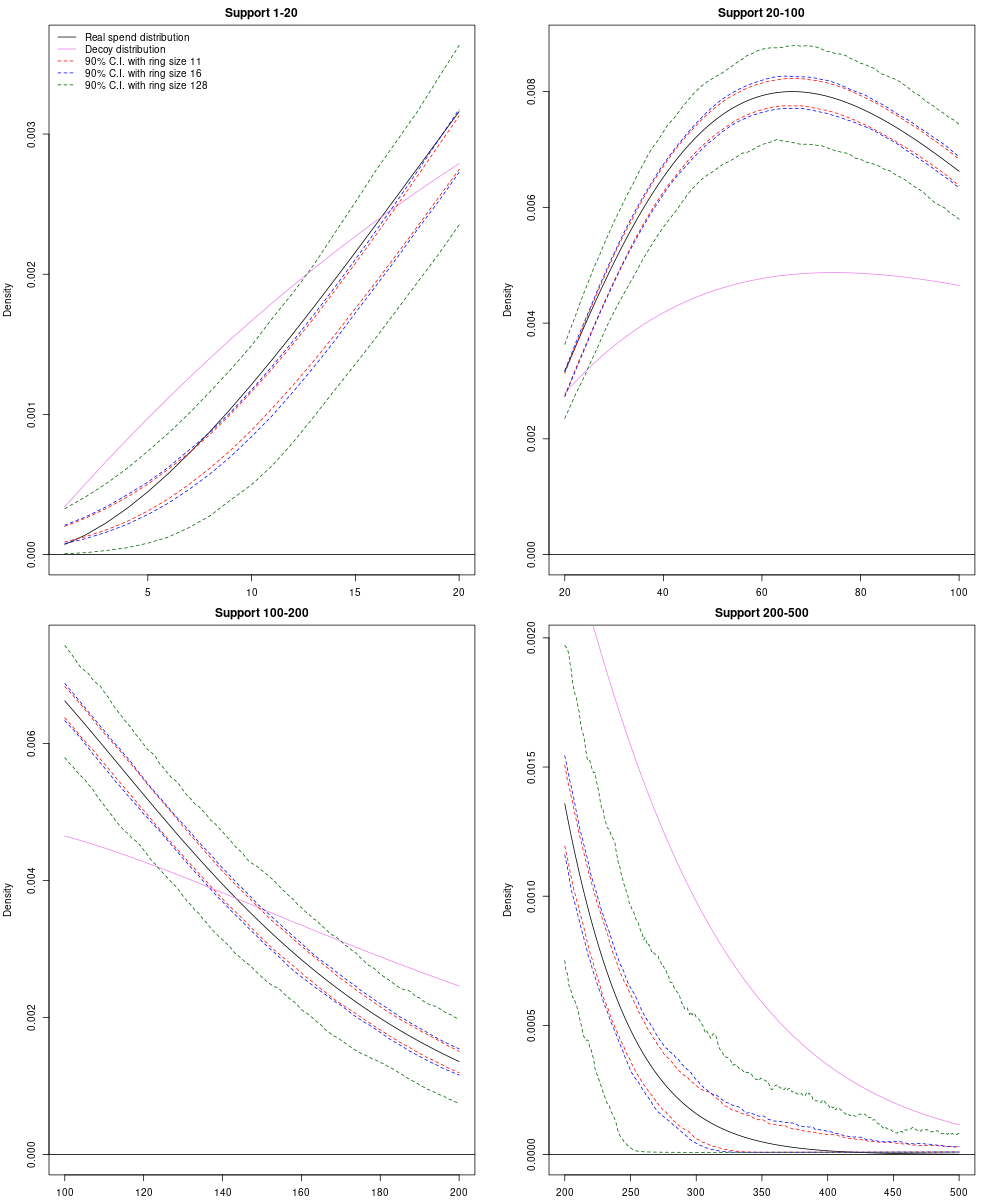
\includegraphics[scale=0.5]{images/patra-sen-monte-carlo}\label{figure-patra-sen-monte-carlo-plots}
\end{figure}

The first thing to notice in these plots is that the confidence intervals
when ring size is 16 are only slightly larger than when ring size
is 11. I calculated the median of the width of all confidence intervals
when $x\in\{20,21,\dots,200\}$ for ring size 11, 16, and 128 to generate
a summary statistic for comparison. According to this median, the
confidence interval for ring size 16 was only 14 percent larger than
for ring size 11. However, precision suffered quite a bit when ring
size rose to 128: the confidence interval with ring size 128 was 212
percent wider than with ring size 16.

Another thing to notice is the estimator's apparent bias in the support
range 1 to 20. As I have mentioned before, some bias is generally
unavoidable with nonparametric kernel density estimators. Looking
carefully at the bias here, it is notable that the estimator is \textit{downward}
biased when the decoy distribution is greater than the real spend
age distribution. My intuition tells me that the bias probably is
not being caused by the density of decoy distribution; if it were,
I would expect an upward --- not downward --- bias in this range
of the support. The bias may be due to the typical bias with kernel
smoothing or some effect of the imposing the monotonicity constraint
on the CDF as in equation (\ref{eq:patra-sen-shape-constrained}).
In general, bias correction procedures are possible, but in practice
they are often avoided since they usually increase the variance of
estimators too much.

Despite the analysis above, we still cannot say with certainty whether
a rise in ring size from 11 to 16 increases or decreases the precision
of my proposed two-step estimator. This is for two reasons. First,
the confidence interval of the first step's estimator may shrink by
64 percent and the confidence interval of the second step's estimator
may expand by only 14 percent, but we cannot know which effect dominates
without knowing the initial confidence interval widths for both estimators
at ring size 11. If the confidence interval of the first step estimator
is very small to begin with and the confidence interval of the second
step estimator is very large, then 14 percent of a large number could
be much bigger than 64 percent of a small one.

The second reason is the general complication of variance estimation
in two-step models discussed in \cite{Murphy1985} and related work.
Unfortunately, the answer to this overall question will have to wait
for the full bootstrap or Monte Carlo estimations. To be clear, bootstrapping
and Monte Carlo estimates for two-step estimators must do the (re)sampling
at the first step and then carry that same sample to the second step
estimate, then resample again at the first step for the next iteration.

Bootstrap-based confidence intervals involve a special challenge with
finite mixture models. \cite{Bonhomme2016} explains:
\begin{quote}
We note that, although it must be taken care of in our simulations,
label swapping does not cause any complications for estimation and
inference based on our approach. Label swapping does present an important
challenge for inference methods based on resampling algorithms such
as the bootstrap or jackknife, and on Markov chain Monte Carlo procedures
(see, for example, Stephens (2000)).
\end{quote}
We need to be able to say that the $k$th $F_{k}$ estimated distribution
in the first step is associated with the $k$th decoy selection algorithm
for estimation in the second step. It is perhaps not too difficult
to do this when a human can examine a single estimate. Bootstrapping
involves many such estimates; I would aim for 1,000 for OSPEAD. Therefore,
some automated way of labeling is recommended. \cite{Bonhomme2016}
describe their own method to avoid label-swapping in their Monte Carlo
simulations:
\begin{quote}
To deal with label swapping in our simulation study we proceed as
follows. In each replication we first estimate the mean of each component.
We then label the estimated component with the smallest estimated
mean as the first mixture component. We carefully checked for label
swapping and found no mix-up.
\end{quote}
The mean of distributions is not very meaningful nor specific in our
setting. Here I tentatively develop two methods that may work alone
or combined to perform automated labeling. The first is to simply
assume that the mixing proportions $\omega_{k}$ would remain stable
in each bootstrap iteration. My hypothesis is that most transactions
are being constructed with the standard \texttt{wallet2} DSA, followed
by the MyMonero DSA as the second most prevalent. We will have to
see what the data tells us to confirm or invalidate that hypothesis.

The second possible approach to automated labeling involves enforcement
of one of the probability axioms: that probability cannot be negative.
The idea is similar to the imposition of monotonicity of the CDF in
equation (\ref{eq:patra-sen-shape-constrained}) from the Patra-Sen
Inversion Estimator. Once a specified DSA distribution is subtracted
from the mixture distribution $F_{k}$, the remaining portion is the
estimate of the real spend age distribution $\hat{F}_{k,S}$ (which
is the label we care about). Of course, due to sampling error some
portion of the corresponding estimated real spend age distribution
$\hat{F}_{k,S}$ may appear as negative; this suggest a statistical
test should be developed, or at least a heuristic. As ring size increases,
this type of automated labeling should get more accurate since there
is less flexibility in the thickness of the real spend age distribution
$F_{k,S}$ as a proportion of the component distribution $F_{k}$.

\subsection{Variance of the Estimator of the Number of Distribution Components
$\boldsymbol{K}$}

The estimator for the number of distribution components $K$ is also
subject to sampling error. \cite{KwonMbakop2021} do not give a way
to compute their estimator's variance or confidence intervals. Bootstrapping
could be a reasonable strategy because it is usually valid even when
the parameter space is discrete \cite{newton1996bootstrapping}. The
parameter space of $K$ is the natural numbers. However, my recommendation
would be to ignore the variance of $\hat{K}$ and to use the (weekly)
estimate of $K$ as its true value because:
\begin{enumerate}
\item $K$ is discrete and probably less than 10. Therefore, the practical
variance of $\hat{K}$ is probably negligible given our sample sizes.
\item A proper bootstrap procedure for $\hat{K}$ creates special problems
for the downstream estimators. Say a bootstrap estimate of $K$ produces
varied estimates of $K$, which anyway would be the whole point of
computing a bootstrap iteration: to estimate the variability of $\hat{K}$.
Then some of the downstream bootstrap estimates of the Bonhomme-Jochmans-Robin
Estimator and the Patra-Sen Inversion Estimator would have a varied
number of estimated components. Then combining those estimates for
bootstrap confidence intervals would result in some ``missing''
and ``extra'' components, greatly complicating valid statistical
inference.
\item The estimator described in \cite{KwonMbakop2021} is computationally
expensive. If bootstrapped, the procedure would have to be done about
1,000 times for each week of data rather than a single time for each
week.
\end{enumerate}

\subsection{Options for Confidence Interval Estimation\label{subsec:Options-for-Confidence-Interval-Estimation}}

My recommendation is to perform about 1,000 nonparametric bootstrap
iterations, starting each iteration from the first step and then passing
the results of the first step to the second step in each iteration.
A nonparametric bootstrap, also known as a case resampling bootstrap,
requires the fewest assumptions about our model and estimator compared
to other bootstrap subtypes. Setting the number of iterations to 1,000
should provide enough information to calculate confidence intervals
with good coverage.\footnote{``Coverage'' used with this meaning: \href{https://en.wikipedia.org/wiki/Coverage_probability}{https://en.wikipedia.org/wiki/Coverage\_probability}}
If the computation is very expensive, then we could settle for 100
iterations. Computation of a closed-form asymptotic confidence interval
is not really an option due both to the two-step nature of the estimator
(as \cite{Murphy1985} warn) and because there is not yet a closed-form
expression for the variance of the Patra-Sen Inversion Estimator.

Another option would be to not estimate any confidence intervals and
just expect that the consistency properties of the estimator will
give us a good estimate. As a statistician, having no metric of precision
at all would make me nervous. Granted, the sample size is quite large.

\section{Sampling Strategy and Data Features that Support Estimation\label{sec:Sampling-Strategy}}

Earlier I said that we have no ``ground truth'' about the different
distribution components $F_{k}$. Even with no ground truth, the data
has certain features that can serve as a check on the estimation.

\begin{wraptable}{O}{0.24\columnwidth}%
\caption{Transactions Per Day Around the Hard Fork}

\label{wrap:table-hard-for-tx-volume}

\begin{tabular}{|c|r|}
\hline 
Date & Transactions\tabularnewline
\hline 
\hline 
2022-08-06 & 21,315\tabularnewline
\hline 
2022-08-07 & 23.297\tabularnewline
\hline 
2022-08-08 & 29,083\tabularnewline
\hline 
2022-08-09 & 27,178\tabularnewline
\hline 
2022-08-10 & 32,995\tabularnewline
\hline 
2022-08-11 & 25,566\tabularnewline
\hline 
2022-08-12 & 61,305\tabularnewline
\hline 
2022-08-13 & 47,536\tabularnewline
\hline 
2022-08-14 & 9,288\tabularnewline
\hline 
2022-08-15 & 18,289\tabularnewline
\hline 
2022-08-16 & 20,555\tabularnewline
\hline 
2022-08-17 & 27,398\tabularnewline
\hline 
2022-08-18 & 29,639\tabularnewline
\hline 
2022-08-19 & 40,914\tabularnewline
\hline 
2022-08-20 & 23,031\tabularnewline
\hline 
2022-08-21 & 20,702\tabularnewline
\hline 
\end{tabular}

Source: \texttt{monero-blockchain-stats}\end{wraptable}%

The plan is to take each week from September 1st, 2021 to October
31, 2022 as a sample. Monero version 0.17.2.3, released September
1, 2021 was the last time that the standard decoy selection algorithm
was changed. Starting the sample in September 2021 would also avoid
the apparent July-August 2021 flood incident that distorted the ring
member age distribution (\cite{Krawiec-Thayer2021}).

There is a clear weekly cycle in the on-chain transaction volume data.
Taking each week as the estimation unit would avoid the need to deal
with the cycles explicitly. The average number of rings (i.e. transaction
inputs) per week since September 2021 has been about 375,000, according
to the \texttt{monero-blockchain-stats} command line utility. This
sample size is probably large enough for acceptable precision of my
proposed estimator. Two-step estimators tend to have larger variance.
The fact that there is a nonparametric kernel estimator involved also
raises variance. If 375,000 observations are not enough, then we can
take samples 4 weeks at a time, making the sample size 1.5 million
rings. It is crucial to break the sample into time units rather than
pooling the entire sample together because the real spend age distribution
is expected to change over time.

\subsection{Leveraging the Hard Fork}

I want to have at least two months of post-hard fork data for a few
different reasons. In my OSPEAD CCS proposal I wrote\footnote{\href{https://ccs.getmonero.org/proposals/Rucknium-OSPEAD-Fortifying-Monero-Against-Statistical-Attack.html}{https://ccs.getmonero.org/proposals/Rucknium-OSPEAD-Fortifying-Monero-Against-Statistical-Attack.html}}: 
\begin{quote}
The upcoming hard fork, which does not yet have a fixed date, will
include an increase in the ring size. The discontinuity that the hard
fork creates can be leveraged to better understand how ring signatures
work in pratcice {[}sic{]} on the Monero blockchain. Therefore, some
of the research work will occur after the hard fork.
\end{quote}
First, it is likely that the larger ring size will shrink the confidence
intervals of the estimates, as I discussed in \textbf{Section \ref{sec:Confidence-Interval-Estimation}
Confidence Interval Estimation}. Second, the hard fork caused user
and software disruption that could generate ``cleaner'' estimates.
Table \ref{wrap:table-hard-for-tx-volume} lists the daily on-chain
transaction volume around the time of the hard fork. The day before
the August 13 hard fork, transaction volume rose to about double normal
levels. The day after the hard fork, transaction volume plummeted
by about 2/3rds.

A large number of wallet implementations did not update in time for
the hard fork. Until they were updated, no transactions constructed
from those wallets would have appeared on the blockchain. Some of
these wallets are known to use non-standard decoy selection algorithms,
such as MyMonero, Edge, and Exodus.\footnote{\href{https://github.com/monero-project/research-lab/issues/99}{https://github.com/monero-project/research-lab/issues/99}}
The decoy selection algorithms of some of the other wallets is unknown.
Table \ref{table-hardfork-wallet-compatibility} contains the approximate
dates that some of these wallets could begin constructing valid transactions
again. During the period of time that these wallets were out of commission,
the proportion of transactions on the blockchain with the standard
decoy selection algorithm, i.e. the mixing proportion $\omega_{wallet2}$
in Equation (\ref{eq:OSPEAD-complete-real-spend-model}), would have
been much higher. Therefore, it would likely be easier to estimate
$F_{wallet2}$ without the distracting other components $F_{k}$ during
this immediate post-hardfork period.

\begin{table}
\caption{Delayed Hardfork-compatible Wallets as of August 30, 2022}

\label{table-hardfork-wallet-compatibility}

\begin{tabular}{|l|l|l|}
\hline 
Fix date & Wallet & Source\tabularnewline
\hline 
\hline 
August 19 & WooKey & {\tiny{}\href{https://github.com/WooKeyWallet/monero-wallet-android-app/releases/tag/v2.2.1}{https://github.com/WooKeyWallet/monero-wallet-android-app/releases/tag/v2.2.1}}\tabularnewline
\hline 
August 25 & Exodus & {\tiny{}\href{https://twitter.com/exodus_io/status/1562918301181034496}{https://twitter.com/exodus\_io/status/1562918301181034496}}\tabularnewline
\hline 
August 27 & Edge & {\tiny{}\href{https://twitter.com/EdgeWallet/status/1563584457361149952}{https://twitter.com/EdgeWallet/status/1563584457361149952}}\tabularnewline
\hline 
August 29 & MyMonero & {\tiny{}\href{https://twitter.com/MyMonero/status/1564149853478760448}{https://twitter.com/MyMonero/status/1564149853478760448}}\tabularnewline
\hline 
Not fixed & Atomic & {\tiny{}\href{https://www.reddit.com/r/atomicwallet/comments/x0w1jr/xmr_balance_showing_zero_i_sent_a_transfer_a_few/}{https://www.reddit.com/r/atomicwallet/comments/x0w1jr/xmr\_balance\_showing\_zero\_i\_sent\_a\_transfer\_a\_few/}}\tabularnewline
\hline 
Not fixed & Coinomi & {\tiny{}\href{https://www.reddit.com/r/COINOMI/comments/wrqvw7/monero_node_is_down_need_to_export_the_mnemonic/}{https://www.reddit.com/r/COINOMI/comments/wrqvw7/monero\_node\_is\_down\_need\_to\_export\_the\_mnemonic/}}\tabularnewline
\hline 
Not fixed & Guarda & {\tiny{}\href{https://libera.monerologs.net/monero-dev/20220831\#c143060}{https://libera.monerologs.net/monero-dev/20220831\#c143060}}\tabularnewline
\hline 
Not fixed & Zelcore & {\tiny{}\href{https://twitter.com/CactusHashAZ/status/1564020934482178048\#m}{https://twitter.com/CactusHashAZ/status/1564020934482178048\#m}}\tabularnewline
\hline 
\end{tabular}
\end{table}


\subsection{MyMonero Fee Fingerprinting\label{subsec:MyMonero-Fee-Fingerprinting}}

jberman discovered that the MyMonero wallet used a method to calculate
transaction fees that is different from \texttt{wallet2}'s method.\footnote{\href{https://github.com/mymonero/mymonero-core-cpp/pull/36}{https://github.com/mymonero/mymonero-core-cpp/pull/36}}
jberman concluded, ``Thus, this difference from wallet2 should be
fingerprintable on chain.'' MyMonero also uses a distinct decoy selection
algorithm.\footnote{\href{https://www.getmonero.org/2021/09/20/post-mortem-of-decoy-selection-bugs.html}{https://www.getmonero.org/2021/09/20/post-mortem-of-decoy-selection-bugs.html}}
The fee fingerprint can be used in two ways. First, the proportion
of MyMonero transactions $\omega_{MyMonero}$ in Equation (\ref{eq:OSPEAD-complete-real-spend-model})
can be calculated exactly for each week rather than estimated with
the Bonhomme-Jochmans-Robin estimator. This can serve as a ``ground
truth'' check on the estimated $\hat{\omega}_{MyMonero}$ that would
hopefully reveal any problems with the Bonhomme-Jochmans-Robin estimator
in this setting.

The second way that the MyMonero fee fingerprinting could be useful
is in partitioning the sample. If the MyMonero component of the mixture
distribution is completely excluded from the first step estimate,
then a certain source of noise is removed. We could exclude these
MyMonero transactions and be done with it if we wanted to construct
the OSPEAD decoy selection algorithm based only on the real spend
age distribution of users of the \texttt{wallet2} DSA. If we wanted
to use the combined \texttt{wallet2} and MyMonero real spend age distribution
as envisaged in equation (\ref{eq:wallet2-mymonero-combined-dsa}),
then we could still exclude MyMonero from the main estimation, but
then take the MyMonero-only sample and apply the Patra-Sen Inversion
Estimator to it directly, skipping the first step Bonhomme-Jochmans-Robin
estimator.

\subsection{Nonstandard Wallets are Nonstandard in Multiple Ways}

The sample partitioning idea can be applied with more wallets than
just MyMonero. Wallets with a nonstandard DSA are also more likely
to have nonstandard fee calculation, \texttt{tx\_extra} contents,
and possibly other transaction uniformity defects. Through querying
databases provided by neptune I have tentatively discovered some \texttt{tx\_extra}
formats associated with nonstandard DSAs. 

Once labeled as such, those transactions can be excluded from the
estimation because they contribute only noise. With the estimation
approach I have outlined above, we can only recover the real spend
age distribution from transactions that use a known decoy selection
algorithm. If a wallet implementation is using an unknown nonstandard
DSA and distinguishes its transactions with other nonstandrad features,
its transactions can be removed from the sample before estimation.

\subsection{\texttt{wallet2} Integer Truncation Bug}

Between Monero versions v0.14.1.0 and v0.17.2.2, \texttt{wallet2}'s
DSA would integer-truncate a value that dictated the spread of the
decoy distribution. This triggered a discontinuity in the distribution
at the point in time that the value would be truncated to the next
integer. The triggering is apparent at approximate block height 2,381,000
in June 2021 in some of the plots of \cite{Krawiec-Thayer2021}. I
do not plan to investigate the trigger point since the reward is probably
not worth the effort. If we wanted to investigate it, would could
get an approximate number for the proportion of transaction constructed
with \texttt{wallet2} around the time of the trucation trigger.

\section{Future Work to Improve the Two-Step Estimator\label{sec:Future-Work-to-Improve-the-Two-Step-Estimator}}

A general note about estimators: If a single valid (i.e. consistent)
estimator of a particular estimand exists, then multiple valid estimators
exist almost always. In general what distinguishes the estimators
may be the assumptions required for their validity and their variance
and bias. My proposed two-step estimator is probably not the lowest-variance
estimator of the estimand. The estimator ``leaves information on
the table'' in a number of ways. In general, when more true information
(do not impose false assumptions if avoidable!) about the structure
of the statistical problem is considered by the estimator, its estimates
become more precise. For example, when more true over-identifying
restrictions are imposed by Generalized Method of Moments estimators,
variance usually falls. I give three ways that the precision of the
estimator can be improved by leveraging more information.

First of all, my proposed estimator does not use the fact that all
rings in the same transaction almost certainly use the same decoy
selection algorithm and therefore all belong to the same $F_{k}$component.
(Note, however, that rings can be cached when a transaction is first
constructed but not broadcast, freezing the ring in time.)\footnote{\href{https://libera.monerologs.net/monero-dev/20220622\#c111774}{https://libera.monerologs.net/monero-dev/20220622\#c111774}}
Every estimator that I have reviewed that attempts to estimate mixture
models with repeated measurements nonparametrically, i.e. that attempts
to estimate the model of Equation (\ref{eq:Bonhomme2016-main-model}),
has an equal number of observations for repeated measurements. If
we could take into account the hierarchical transaction structure
of the data, then the number of repeated measures $M+1$ could vary
according to the number of rings in a given transaction. As seen in
\textbf{Section \ref{sec:Confidence-Interval-Estimation} Confidence
Interval Estimation}, a larger $M+1$ increases the precision of the
Bonhomme-Jochmans-Robin estimator.

The second way is to convert the two-step estimator into a single-step
joint estimator in which a single objective function is optimized
to produce estimates in both steps simultaneously. Among maximum livelihood
estimators, such an estimator is known as ``Full Information Maximum
Likelihood'' (FIML) \cite{Murphy1985}. Creating such an estimator
would likely require a great deal of effort and skill in theoretical
statistics.

The third way may or may not be mutually exclusive with the second.
In the first step, we do not exploit the fact that we know quite a
bit about several of the $F_{k}$ components --- specifically, that
the component distributions have an admixture/contamination structure
with a known parametric form of the largest sub-component (i.e. the
DSA) for several of the components. There may be a way to include
this information from the second step into the first step estimator.

There are a few recent papers on using Bayesian methods to model ``mixture
of mixtures'' or ``hierarchical mixture models''(\cite{malsiner2017identifying},
\cite{Argiento2020}, \cite{Fruhwirth2021}).

I consider these possible improvements to the estimator to be out
of scope for this initial OSPEAD CCS. The gain is not worth the effort
at this time.

\section{Rucknium Ratio Attack/MAP Decoder/Discriminant Analysis\label{sec:Rucknium-Ratio-Attack}}

An inebriated Homer Simpson once said, ``To alcohol! The cause of,
and solution to, all of life's problems.'' Similar to alcohol, an
estimate of the real spend age distribution is the cause of, and solution
to, many of Monero's statistical attack problems.

The potency of statistical attacks is a critical overall factor influencing
the disclosure decision in \textbf{Section \ref{sec:Disclosure-Considerations}
Disclosure Considerations}. \cite{Ronge2021} give the following metrics
of statistical attack potency:
\begin{quote}
\textbf{Definition 3.1.} \textit{The guessing probability of }$\mathsf{X}$\textit{
is}

\[
\mathrm{Guess}(\mathsf{X})\coloneqq\underset{X}{\max}\Pr\left[\mathsf{X}=X\right].
\]

This gives an upper bound on the probability than an (unbounded) adversary
can ``guess'' the value of the random variable $\mathsf{X}$ correctly.

\textbf{Definition 3.2.} \textit{The (average) conditional guessing
probability of }$\mathsf{X}$\textit{ given $\mathsf{Y}$ is defined
as}

\[
\mathrm{Guess}(\mathsf{X}|\mathsf{Y})\coloneqq\sum_{Y}\Pr\left[\mathsf{Y}=Y\right]\underset{X}{\max}\Pr\left[\mathsf{X}=X|\mathsf{Y}=Y\right].
\]

This gives an upper bound on the probability that an (unbounded) adversary
``guesses'' the value of the random variable $\mathsf{X}$ correctly
when given a sample of $\mathsf{Y}$....

\textbf{Theorem 4.4.} \textit{Let $\mathcal{A}$ be any computationally
unbounded adversary, who inputs a ring $\Pi(S)$ (where $\Pi$ {[}the
ring sampler, i.e. Decoy Selection Algorithm,{]} is possibly subverted
by $\mathcal{A}$) and some leakage $\Lambda(S)$, where $S$ is sampled
from the distribution $\mathcal{S}$ (possibly influenced or specified
by $\mathcal{A}$), and outputs a guess $S'$. The probability of
$\mathcal{A}$ correctly guessing the signer $S$, i.e., $S'=S$,
is upper bounded by}

\begin{equation}
\mathrm{Guess}\left(\mathsf{S}|\Pi(\mathsf{S}),\Lambda(\mathsf{S})\right)=2^{-\alpha(\mathsf{S},\Pi,\Lambda)}.\label{eq:Ronge-et-al-2021-signer-guessing}
\end{equation}
\end{quote}
The right hand side of Equation (\ref{eq:Ronge-et-al-2021-signer-guessing})
is not important for this discussion. $\Lambda(\mathsf{S})$, which
represents side-channel information like view keys, logs of centralized
exchanges, EAE/EABE attacks, etc., is out of scope. Therefore, we
will deal with the simpler $\mathrm{Guess}\left(\mathsf{S}|\Pi(\mathsf{S})\right)$.
Possible active attacks on the DSA by adversary \textit{$\mathcal{A}$}
like flooding/black marble attacks are also out of scope.

In my HackerOne submission I performed a Monte Carlo simulation to
approximate the probability of success of the ``Rucknium Ratio Attack''
when the decoy selection algorithm diverges from the real spend age
distribution, where I found $\mathrm{E}\left[\mathrm{\widehat{Guess}}_{RRA}\left(\mathsf{S}|\Pi(\mathsf{S})\right)\right]\approx0.35$.
The Rucknium Ratio Attack guesses that the most likely real spend
is the ring member, compared to all other ring members in a ring,
whose age $x$ is at the maximum ratio $\tfrac{f_{S}\left(x\right)}{f_{D}\left(x\right)}$,
i.e. the ratio of the real spend distribution to the decoy distribution.
Unknown to me at the time, a few months prior \cite{Aeeneh2021} had
published an essentially identical attack they called the ``Maximum
A Posteriori (MAP) Decoder''. They did not attempt to estimate the
empirical potency of the attack because they did not think obtaining
an estimate of the real spend age distribution $f_{S}(x)$ was possible.
I will refer to this attack as the MAP Decoder since it is more descriptive
of the technique and \cite{Aeeneh2021} were first to publish. The
Maximum A Posteriori Decoder is related to the Maximum A Posteriori
(MAP) \textit{estimator}. The MAP estimator find the statistical mode
(i.e. the most frequent value) of the posterior distribution for a
particular distribution \cite{Bassett2019}. The MAP Decoder finds
the most frequent value for the ratio of two distributions.

In their Equation 13, \cite{Aeeneh2021} state the closed-form expression
for the error probability of their attack. I will translate it into
our notation. $M$ is the number of decoys. Let $\boldsymbol{R}=\left\{ r_{1},r_{2},\dots,r_{M+1}\right\} $
be the set of ring members that have corresponding block height $\boldsymbol{B}=\left\{ b_{1},b_{2},\dots,b_{M+1}\right\} $.
Without loss of generality, assume that the real spend is $r_{1}$.
Let $J$ be the number of blocks that have RingCT outputs. In other
words, $J$ is the maximum age of a possible ring member, in units
of block height. Then when the real spend $r_{1}$ is at block height
$b_{1}$, the probability that the MAP Decoder correctly guesses the
real spend is:

\begin{equation}
\left(\sum_{j=1}^{J}f_{D}\left(j\right)\mathbf{1}\left\{ \tfrac{f_{S}\left(j\right)}{f_{D}\left(j\right)}<\tfrac{f_{S}\left(b_{1}\right)}{f_{D}\left(b_{1}\right)}\right\} \right)^{M}\label{eq:MAP-Decoder-Success-Single-Ring}
\end{equation}

The $\mathbf{1}\left\{ \tfrac{f_{S}\left(j\right)}{f_{D}\left(j\right)}<\tfrac{f_{S}\left(b_{1}\right)}{f_{D}\left(b_{1}\right)}\right\} $
indicator function term checks if a potential decoy drawn from the
$j$th block would have a lower $\tfrac{f_{S}\left(x\right)}{f_{D}\left(x\right)}$
value than the real spend $r_{1}$. If the potential decoy does not
have a lower value that the real spend, then the real spend would
not be guessed by the MAP Decoder. The $f_{D}\left(j\right)$ weights
each $\mathbf{1}\left\{ \tfrac{f_{S}\left(j\right)}{f_{D}\left(j\right)}<\tfrac{f_{S}\left(b_{1}\right)}{f_{D}\left(b_{1}\right)}\right\} $
term by the probability that the decoy selection algorithm would choose
a decoy from that $j$th block height. Then the $\sum_{j=1}^{J}$
operator sums each weighted indicator function for every possible
$J$ blocks that a decoy could be chosen from. Then for the whole
expression we need to calculate the joint probability for every decoy
selected in the ring. We can take the $M$th power of the expression
for $M$ decoys since the decoy selection algorithm (or at least that
of \texttt{wallet2}) chooses decoys in an independent and identically
distributed manner.

Expression \ref{eq:MAP-Decoder-Success-Single-Ring} gives the probability
that the MAP Decoder correctly guesses the real spend for a particular
real spend $r_{1}$ at block height $b_{1}$. To calculate the expectation
of $\mathrm{Guess}_{MAPD}\left(\mathsf{S}|\Pi(\mathsf{S})\right)$
(i.e. the average) over all real spends, we weight Expression \ref{eq:MAP-Decoder-Success-Single-Ring}
by the probability that a user spends from each block height age $f_{S}\left(x\right)$
and then sum: 

\begin{equation}
\mathrm{E}\left[\mathrm{Guess}_{MAPD}\left(\mathsf{S}|\Pi(\mathsf{S})\right)\right]=\sum_{b_{1}=1}^{J}f_{S}\left(b_{1}\right)\left(\sum_{j=1}^{J}f_{D}\left(j\right)\mathbf{1}\left\{ \tfrac{f_{S}\left(j\right)}{f_{D}\left(j\right)}<\tfrac{f_{S}\left(b_{1}\right)}{f_{D}\left(b_{1}\right)}\right\} \right)^{M}\label{eq:MAP-Decoder-Success-Expectation}
\end{equation}

Equation (\ref{eq:MAP-Decoder-Success-Expectation}) apparently requires
summation of $J^{2}$ elements. Given that $J$ is in excess of one
million, computation of (\ref{eq:MAP-Decoder-Success-Expectation})
could be computationally expensive. However, by intelligently ordering
the quantities to be compared, the computational expense can be reduced
by several orders of magnitude. In \texttt{map-decoder-attack-potency.R}
I perform the calculations with a naive implementation and an efficient
one. With estimates of $f_{S}(x)$ and $f_{D}(x)$ from my HackerOne
submission, Equation (\ref{eq:MAP-Decoder-Success-Expectation}) gives
$\mathrm{E}\left[\mathrm{Guess}_{MAPD}\left(\mathsf{S}|\Pi(\mathsf{S})\right)\right]\approx35.43693\%$,
which is within about one hundredth of a percentage point of $35.4512\%$,
the value I found from my original Monte Carlo simulation. When ring
size is 16, $\mathrm{E}\left[\mathrm{Guess}_{MAPD}\left(\mathsf{S}|\Pi(\mathsf{S})\right)\right]\approx30.39\%$
with my HackerOne estimates of $f_{S}(x)$ and $f_{D}(x)$.

It is beneficial to have the Equation (\ref{eq:MAP-Decoder-Success-Expectation})
closed-form expression of $\mathrm{E}\left[\mathrm{Guess}_{MAPD}\left(\mathsf{S}|\Pi(\mathsf{S})\right)\right]$
with an efficient implementation rather than needing to resort to
Monte Carlo simulation. Minimizing $\mathrm{E}\left[\mathrm{Guess}_{MAPD}\left(\mathsf{S}|\Pi(\mathsf{S})\right)\right]$
is one of several criteria that I propose for determining the OSPEAD
decoy selection algorithm later in \textbf{Section \ref{subsec:Maximize-Resistance-to-an-Attack}
Maximize Resistance to an Attack}. For a numerical minimization algorithm
it is much better to have function evaluation computation time measured
in seconds rather than minutes. There are also particular difficulties
(though surmountable) with having the objective function be stochastic
as would be the case with $\mathrm{E}\left[\mathrm{Guess}_{MAPD}\left(\mathsf{S}|\Pi(\mathsf{S})\right)\right]$
estimated with Monte Carlo simulation.

My HackerOne estimate of $\mathrm{E}\left[\mathrm{Guess}_{MAPD}\left(\mathsf{S}|\Pi(\mathsf{S})\right)\right]$
was based on the false simplifying assumption that the \texttt{wallet2}
decoy selection algorithm was the only one being used on the Monero
blockchain, using a simplified version of the Patra-Sen Inversion
Estimator to obtain an estimate of $f_{S}(x)$. My proposed two-step
estimator will produce a consistent estimate of $f_{S}(x)$ under
the assumption that multiple decoy selection algorithms are being
used. A more accurate estimate of $\mathrm{E}\left[\mathrm{Guess}_{MAPD}\left(\mathsf{S}|\Pi(\mathsf{S})\right)\right]$
could be produced from this improved estimate of $f_{S}(x)$. I am
not sure if this more accurate estimate of $\mathrm{E}\left[\mathrm{Guess}_{MAPD}\left(\mathsf{S}|\Pi(\mathsf{S})\right)\right]$
would be greater than or less than the original HackerOne estimate.
There are two factors that cut in opposite directions.

First, the original estimate would have conflated decoys from nonstandard
decoy selection algorithms with real spends, potentially biasing the
estimate of $\mathrm{E}\left[\mathrm{Guess}_{MAPD}\left(\mathsf{S}|\Pi(\mathsf{S})\right)\right]$
upward. The magnitude of this source of bias is dependent on the divergence
between the \texttt{wallet2} DSA and the nonstandard DSAs, plus the
proportion of on-chain transactions that use the nonstandard DSAs.

On the other hand, the original estimate of $\mathrm{E}\left[\mathrm{Guess}_{MAPD}\left(\mathsf{S}|\Pi(\mathsf{S})\right)\right]$
may have been biased downward because it did not take into account
the variability of $f_{S}(x)$ over time. It gave an ``average''
over the time period under consideration. Assume for a moment that
the \texttt{wallet2} DSA performed adequately for the average $f_{s}(x)$
over time. If $f_{s}(x)$ was highly variable from week to week, $\mathrm{E}\left[\mathrm{Guess}_{MAPD}\left(\mathsf{S}|\Pi(\mathsf{S})\right)\right]$
could still be high since the MAP Decoder could exploit the extremes
of each week.

We will not have an improved estimate of $\mathrm{E}\left[\mathrm{Guess}_{MAPD}\left(\mathsf{S}|\Pi(\mathsf{S})\right)\right]$
until we have the improved estimate of $f_{S}(x)$.

\subsection{Attack Optimality}

\cite{Aeeneh2021} claims in their Proposition 4 that the MAP Decoder
attack is optimal in the sense that it minimizes the (guessing) error
probability. If there there is no attack more powerful, then it may
make sense to construct the OSPEAD DSA by minimizing the MAP Decoder
effectiveness as I suggest in \textbf{Section \ref{subsec:Maximize-Resistance-to-an-Attack}
Maximize Resistance to an Attack}. It is not clear to me whether maximizing
resistance to the most powerful attack also maximizes resistance to
a less powerful attack. For example, the ``guess newest heuristic''
of \cite{Kumar2017} and \cite{2018} is a less powerful attack that
exploits \textit{part} of the information about the discrepancy between
$f_{S}(s)$ and $f_{D}(x)$.

In formal terms: Let $\Pi_{MAPD}(\mathsf{S})$ be the DSA that is
constructed to minimize $\mathrm{E}\left[\mathrm{Guess}_{MAPD}\left(\mathsf{S}|\Pi(\mathsf{S})\right)\right]$
(with the constraint that $\Pi_{MAPD}(\mathsf{S})$ is static and
parametric). Let $\Pi_{Alt}(\mathsf{S})$ be some alternative DSA
that does not minimize $\mathrm{E}\left[\mathrm{Guess}_{MAPD}\left(\mathsf{S}|\Pi(\mathsf{S})\right)\right]$.
Let $\mathrm{Guess}_{MAPD_{inferior}}$ be the guessing probability
of an attack $MAPD_{inferior}$ that is inferior to the Map Decoder.
Does there exist a $\Pi_{Alt}(\mathsf{S})$ and $MAPD_{inferior}$
such that

\[
\mathrm{E}\left[\mathrm{Guess}_{MAPD}\left(\mathsf{S}|\Pi_{MAPD}(\mathsf{S})\right)\right]<\mathrm{E}\left[\mathrm{Guess}_{MAPD}\left(\mathsf{S}|\Pi_{Alt}(\mathsf{S})\right)\right]
\]

(which is true by Proposition 4 of \cite{Aeeneh2021}), yet also

\[
\mathrm{E}\left[\mathrm{Guess}_{MAPD_{inferior}}\left(\mathsf{S}|\Pi_{MAPD}(\mathsf{S})\right)\right]>\mathrm{E}\left[\mathrm{Guess}_{MAPD_{inferior}}\left(\mathsf{S}|\Pi_{Alt}(\mathsf{S})\right)\right]?
\]
 

If the answer is in the affirmative and an adversary can implement
$MAPD_{inferior}$ but not $MAPD$, then it could be better to adopt
something other than $\Pi_{MAPD}(\mathsf{S})$ as the new DSA. In
such case, it might be better to use one of the other criteria I develop
in \textbf{Section \ref{sec:Criteria-for-Best-Fit} Criteria for Best
Fit}. That said, in the following discussion I lay out an argument
that the MAP Decoder attack may have deep optimality properties.

My search of the statistics literature suggested that the MAP Decoder/Rucknium
Ratio Attack is just a specific instance of a very old problem and
class of solutions: Discriminant Analysis, a type of supervised classification
(\cite{mclachlan1992discriminant} \cite{FraleyRaftery2002}). As
early as 1951, the year that \cite{FixHodges1989} was originally
written under a U.S. Air Force contract, this problem was consider
to be, ``in a sense, completely solved.'' In 1989 \cite{FixHodges1989}
was finally published in a journal due to its importance. After consistent
estimation of the real spend age distribution, I take our problem
as falling into the category of ``subproblem (i)'' below:
\begin{quote}
The discrimination problem (two population case) may be defined as
follows: a random variable $Z$, of observed value $z$, is distributed
over some space (say, $p$-dimensional) either according to distribution
$F$, or according to distribution $G$. The problem is to decide,
on the basis of $z$, which of the two distributions $Z$ has.

The problem may be classified in various ways into subproblems. One
pertinent method of classification is according to the amount of information
assumed to be available about $F$ and $G$. We may distinguish three
stages:
\begin{quote}
(i) $F$ and $G$ are completely known;

(ii) $F$ and $G$ are known except for the values of one or more
parameters;

(iii) $F$ and $G$ are completely unknown, except possibly for assumption
about the existence of densities, etc.
\end{quote}
Subproblem (i) has been, in a sense, completely solved. The solution
is implicit in the Neyman-Pearson lemma (Neyman \& Pearson, 1936),
and was made explicit by Welch (1939). We may without loss of generality
assume the existence of density functions, say $f$ and $g$, corresponding
to $F$ and $G$, since $F$ and $G$ are absolutely continuous with
respect to $F$ + $G$. If $f$ and $g$ are known, the discrimination
should depend only on $f(z)/g(z)$. An appropriate (positive) constant
$c$ is chosen, and the following rule is observed:
\begin{quote}
if $f(z)/g(z)>c$, we decide in favor of $F$;

if $f(z)/g(z)<c$, we decide in favor of G;

if $f(z)/g(z)=c$, the decision may be made in an arbitrary manner.
\end{quote}
These procedures are known to have optimum properties with regard
to control of probability of misclassification (probability of wrong
decision). We shall refer to this as the 'likelihood ratio procedure',
and denote it by $L(c)$....

The choice of $c$ depends on considerations related to the relative
importance of the two possible errors: saying $Z$ is distributed
according to $G$ when in fact it is distributed to $F$, and conversely.
Two choice of $c$ have been widely advocated:
\begin{quote}
(a) take $c=1$;

(b) choose $c$ so that the two probabilities of error are equal.
\end{quote}
Choice (a) has been called 'logical'; choice (b) yields the minimax
procedure. In this paper we shall not concern ourselves with the choice
of $c$, but shall assume that a given positive $c$ is a datum of
the problem.
\end{quote}
\textit{``If $f$ and $g$ are known, the discrimination should depend
only on $f(z)/g(z)$.'' }This 70-year-old principle is used in the
MAP Decoder attack. The main difference between MAP Decoder and this
passage from \cite{FixHodges1989} is that the inequality criterion
$f(z)/g(z)\gtreqqless c$ is not governed by a constant $c$. In the
MAP Decoder attack, $c$ is variable, determined by the ratio $f(z)/g(z)$
for every other ring member in the ring, i.e. $c=\underset{i}{\max}\{f(z_{i})/g(z_{i})\}$.

\cite{McLachlan2019} give a more general and modern explanation of
the principle, placing it within the framework of finite mixture models:
\begin{quote}
The mixture model give by Equation (\ref{eq:McLachlan-parametric-mixture-model})
can be used to provide a model-based approach to clustering of the
observed data in $\boldsymbol{y}_{obs}$ by conceptualizing that $\boldsymbol{y}_{1},\ldots,\boldsymbol{y}_{n}$
come from a mixture in proportions $\pi_{1,},\ldots,\pi_{g}$ of $g$
groups $G_{1},\ldots,G_{g}$ in which $\boldsymbol{Y}_{j}$ has density
$f_{1}(\boldsymbol{y}_{j};\mathbf{\boldsymbol{\theta}}_{1}),\ldots,f_{g}(\boldsymbol{y}_{j};\boldsymbol{\theta}_{g})$,
respectively. This is irrespective of whether these groups do externally
exist.

For clustering purposes, each component in the mixture model given
by Equation (\ref{eq:McLachlan-parametric-mixture-model}) is usually
taken to correspond to a cluster. The posterior probability that the
$j$th observation $\boldsymbol{y}_{j}$ arose from group $G_{i}$
is given by the fitted posterior probability,

\begin{equation}
\tau_{i}(\boldsymbol{y}_{j};\hat{\boldsymbol{\Psi}})=\hat{\pi}_{i}f_{i}(\boldsymbol{y}_{j};\hat{\boldsymbol{\theta}}_{i})/f_{i}(\boldsymbol{y}_{j};\hat{\boldsymbol{\Psi}})\quad(i=1,\ldots,g;j=1,\ldots,n),\label{eq:discriminant-analysis-McLachlan2019-tau}
\end{equation}

where $\hat{\boldsymbol{\Psi}}$ denotes an estimate of $\boldsymbol{\Psi}$.

A probabilistic clustering of the data $\boldsymbol{y}_{1},\ldots,\boldsymbol{y}_{n}$
into $g$ clusters can be obtained in terms of the fitted posterior
probabilities of component membership $\tau_{i}(\boldsymbol{y}_{j};\hat{\boldsymbol{\Psi}})(i=1,\dots,g)$.

An outright partitioning of the observations into $g$ nonoverlapping
clusters $C_{1},\dots,C_{g}$ is effectuated by assigning each $\boldsymbol{y}_{j}$
to the group $G_{i}$ to which it has the highest estimated posterior
probability of belonging. That is, the $i$th cluster $C_{i}$ contains
those observations $\boldsymbol{y}_{j}$ with $\hat{z}_{ij}=\left(\hat{\mathbf{z}}_{j}\right)_{i}=1$,
where 

\begin{equation}
\begin{array}{cccc}
\hat{z}_{ij} & =1, &  & \mathrm{if}\:i=\arg\underset{h}{\max}\,\hat{\tau}_{h}(\boldsymbol{y}_{j};\hat{\boldsymbol{\Psi}}),\\
 & =0, &  & \mathrm{otherwise.\qquad\qquad\qquad}
\end{array}\label{eq:discriminant-analysis-McLachlan2019-Bayes-rule}
\end{equation}

As the notation implies, $\hat{z}_{ij}$ can be viewed as an estimate
of $z_{ij}$ which, under the assumption that the observations come
from a mixture of $g$ groups $G_{1},\dots,G_{g}$, is defined to
be one or zero according to whether $\boldsymbol{y}_{j}$ did or did
not arise from $G_{i}(i=1,\dots,g)$.

The above rule for assigning the unclassified data points $\boldsymbol{y}_{j}$
to the $g$ groups corresponds to the Bayes rule of allocation in
the supervised classified case with known parameter vector $\boldsymbol{\Psi}$
(\cite{mclachlan1992discriminant}, section 1.3).
\end{quote}
The $\hat{\pi}_{i}$ in equation (\ref{eq:discriminant-analysis-McLachlan2019-tau})
is the estimated mixing proportion of the $i$th density component.
If we were to apply the assignment rule of (\ref{eq:discriminant-analysis-McLachlan2019-Bayes-rule})
to a ring to classify ring members into the real spend and decoy distribution,
the decoy distribution would always be heavily weighted since $\pi_{D}=\tfrac{M}{M+1}$,
where $M$ is the number of decoys. Thus, in many cases all ring members
would be classified as decoys if this particular Bayes rule of allocation
were to be used.

The general idea of this Bayes rule is packaged in a piece of advice
given to physicians about diagnosis of disease: \textquotedblleft When
you hear hoofbeats in the night, look for horses --- not zebras.''\footnote{\href{https://quoteinvestigator.com/2017/11/26/zebras/}{https://quoteinvestigator.com/2017/11/26/zebras/}}
In other words, when you have some limited symptom data that is consistent
with two diseases, i.e. $f_{1}(\boldsymbol{y}_{j};\hat{\boldsymbol{\theta}}_{1})=f_{2}(\boldsymbol{y}_{j};\hat{\boldsymbol{\theta}}_{2})$
for symptom data $\boldsymbol{y}_{j}$ and diseases $1$ and $2$,
choose the diagnosis of the disease that is more prevalent in the
population, i.e. choose the disease with the larger mixing proportion
$\pi_{i}$.

Our problem is different in that we can use information from all $M+1$
observations in a set of repeated measures --- all members of a ring
--- for classification. The general term for this setting is the
``compound decision problem'' \cite{Copas1974}. To extend the metaphor,
we know that there is exactly one zebra in the corral (there is exactly
one real spend in a Monero ring). To re-imagine the MAP Decoder in
the framework of the (\ref{eq:discriminant-analysis-McLachlan2019-Bayes-rule})
assignment rule, we can instead make an assignment (a guess) based
on:

\[
\begin{array}{cccc}
\hat{z}_{ij} & =1, &  & \mathrm{if}\:j=\arg\underset{k}{\max}\,\hat{\tau}_{i}(\boldsymbol{y}_{k};\hat{\boldsymbol{\Psi}}),\\
 & =0, &  & \mathrm{otherwise.\qquad\qquad\qquad}
\end{array}
\]

In other words, apply the decision rule over the rows ($i$th dimension
where $i$ denotes the distribution component) of the $\hat{z}_{ij}$
matrix rather than over the columns ($j$th dimension where $j$ denotes
the observation). Thus, we consider each distribution (in our problem
the two distributions: real and decoy) and then assign the most likely
observation (ring member) to that distribution --- we can ignore
the decoy assignment since we are interested in the assignment of
the real spend --- rather than considering each observation and assigning
the most likely distribution to it.

With a quick search I have not found a paper that covers our exact
case of a compound decision problem in which the proportion of the
sample belonging to each component is known exactly. Diving further
into this corner of statistics may uncover more properties of the
MAP Decoder such as how to maximize its error rate when one of the
distributions, i.e. the decoy distribution, can be partially manipulated.

To conclude, it is likely that the MAP Decoder attack is the most
dangerous statistical attack that exploits the timestamp information
on the Monero blockchain. Therefore, I am personally leaning toward
using the minimization of $\mathrm{E}\left[\mathrm{Guess}_{MAPD}\left(\mathsf{S}|\Pi(\mathsf{S})\right)\right]$
as the criteria to select the OSPEAD decoy selection algorithm.

\section{Postestimation Classification of On-Chain Rings into DSAs\label{sec:Postestimation-Classification}}

Given estimates of the mixture model components $F_{k}$, is it possible
to probabilistically classify rings on the Monero blockchain according
to their associated decoy selection algorithm? I believe it may be
possible. There are two main reasons we might be interested in doing
this.

The first is to better understand the degree of defects in transaction
uniformity on the blockchain --- the ``anonymity puddles.'' Transaction
uniformity defects themselves can be used as ammunition in statistical
attacks against Monero user privacy. The second reason is to evaluate
the safety of implementing an OSPEAD-derived DSA in a new release
of the Monero \texttt{wallet2} software at a time other than a hard
fork. It could be possible to probabilistically distinguish between
transactions constructed with the new DSA and the old DSA, which could
endanger user privacy. Without a hard fork, users who use the GUI
or CLI wallet and wallet developers who use \texttt{wallet2} to construct
transactions are not required to upgrade to the new version. The question
is whether the cure would be worse than the disease:

\begin{equation}
\Pr\left(MAPD_{wallet2\_DSA}\right)\overset{?}{\lessgtr}\Pr\left(MAPD_{OSPEAD\_DSA}\cup Classifier_{wallet2\_DSA/OSPEAD\_DSA}\right)\label{eq:classification-risk}
\end{equation}

where $MAPD_{wallet2\_DSA}$ is the event that the real spend is guessed
by the MAP Decoder attack with the existing DSA, $MAPD_{OSPEAD\_DSA}$
is the same with the OSPEAD-derived DSA, and $Classifier_{wallet2\_DSA/OSPEAD\_DSA}$
is the event that a DSA-based classifier correctly guesses the real
spend by distinguishing between transactions using the existing DSA
and the OSPEAD-derived DSA. Further data analysis is required because
the direction of the inequality in (\ref{eq:classification-risk})
must be resolved empirically rather than theoretically.

Inequality (\ref{eq:classification-risk}) is not very formal. It
does not consider the ``adoption curve'' over time of users updating
to a new \texttt{wallet2} version. A more complete decision criteria
would consider the risk over time and an educated guess about the
adoption curve. An educated guess could be based on an estimate of
the rate of adoption of the bug fixes to the decoy selection algorithm
written by jberman in 2021, using the Bonhomme-Jochmans-Robin estimator.

There are a few candidate techniques for probabilistic classification
of rings using their repeated measures structure. \cite{Bagui2006}
describe the state of the literature as of 2006:
\begin{quote}
Various nonparametric procedures are available in situations where
independent repeated measurements are available on the entity to be
classified; they have been considered by Das Gupta {[}7{]}, Hudimoto
{[}15{]}, Kanazawa {[}18{]}, Gupta and Kim {[}13{]}, Lin {[}17{]},
Govindarajulu and Gupta {[}12{]}, and Haack and Govindarajulu {[}14{]}
among others. DasGupta {[}7{]} proposed an allocation rule using the
Wilcoxon statistic. Govindarajulu and Gupta {[}12{]} considered an
allocation rule based on linear rank statistics for the $s$-group
problem....

Bagui {[}2{]} considered the problem of classification of $m$ independent
multiple observations under the mixture sampling scheme which is common
in prospective studies and diagnostic situations. Bagui et al. {[}3{]}
proposed the allocation of multiple observations using a sub-sample
approach under mixture sampling. Bagui and Mehra {[}4{]} used a rank
nearest neighbor (RNN) classification rule to classify univariate
independent multiple observations between two classes. The present
article deals with the classification of $m$ independent (multivariate)
multiple observations under a separate (or conditional) sampling scheme.
\end{quote}
I consider exploration of ring classification to be out of scope of
this OSPEAD CCS. It would require much additional research. Future
work could cover this ground.

\section{Disclosure Considerations\label{sec:Disclosure-Considerations}}

Given the potential threat to retroactive user privacy of an estimate
of the real spend age distribution combined with the MAP Decoder attack,
there is a question of whether to disclose the estimator. A sophisticated
adversary who pays close attention likely would already be aware of
the MAP Decoder attack since it was published in \cite{Aeeneh2021}.
All that is missing is an estimate of the real spend age distribution.
The decoy selection algorithm of course would be plainly visible in
Monero's source code, so it is a matter of disclosing how the parameters
of the algorithm was chosen.

The process to decide on disclosure is not very formal at this point.
It is not clear what exact body of individuals plays the role of deciding
to disclose or not. After I completed my initial investigations in
August/September 2021 I submitted my findings through HackerOne in
compliance with Monero's Vulnerability Response Process. After discussion,
the VRP manager deferred to my judgment about whether to publicly
disclose immediately. I chose not to disclose because the risk to
user privacy was still not completely understood and we had no fix
ready. It would make sense for the revoew panel to give input on about
the advisability of disclosure.

As I stated in Section \ref{sec:Rucknium-Ratio-Attack}, we will not
have an improved estimate of the potency of the MAP Decoder attack
until we have the improved estimate of the real spend distribution
Therefore, we do not need to make a final call at this point in time.
Below I discuss some pros and cons of disclosure.

\subsection{Pros}

\subsubsection{Greater peer review of OSPEAD}

Disclosure would enable wider peer review of my proposed solution.
Disclosure of this document and my HackerOne submission would potentially
put more eyes on the OSPEAD estimator. Furthermore, if we choose disclosure
I am willing to prepare a manuscript for submission to a privacy-focused
journal for a traditional peer review process. We could then benefit
from suggested improvements to OSPEAD.

\subsubsection{More attention to this research area}

Many papers such as \cite{Egger2022}\cite{Ronge2021}, and \cite{Yu2019}
have suggested a ``partitioning'' (i.e. a single bin) DSA, partially
since they did not think it was feasible to estimate the real spend
age distribution. Disclosure of OSPEAD could revitalize research on
mimicking DSAs.

Nonparametric mixture models are an active area of statistical research.
With disclosure, we might be able to catch the interest of theoretical
statisticians to help us refine and strengthen the OSPEAD approach.

An estimate of the real spend age distribution may also be useful
to potential future research on churning.

\subsubsection{User trust}

Community trust in the security of the code and the privacy of its
protocol is essential. Many community members might not accept concealment
of any part of the process of how certain designed decisions were
determined. When I submitted my CCS proposal, my suggestion that parts
of OSPEAD be remain a secret was very controversial.\footnote{\href{https://www.reddit.com/r/Monero/comments/py8ub3/ccs_proposal_ospead_fortifying_monero_against/}{https://www.reddit.com/r/Monero/comments/py8ub3/ccs\_proposal\_ospead\_fortifying\_monero\_against/}}

Community members' concern is not without some basis in reality. In
the past, malicious parties have used ``suggested'' cryptographic
parameters to effectively create backdoors, such as the suspected
NSA backdoor in Dual\_EC\_DRBG.\footnote{\href{https://en.wikipedia.org/wiki/Dual_EC_DRBG}{https://en.wikipedia.org/wiki/Dual\_EC\_DRBG}}

On the other hand, there is precedent for publication of certain security
parameters without explicit justification because the justification
would reveal attacks, such as with the discovery of differential cryptanalysis:\footnote{\href{https://en.wikipedia.org/wiki/Differential_cryptanalysis}{https://en.wikipedia.org/wiki/Differential\_cryptanalysis}}
\begin{quote}
The discovery of differential cryptanalysis is generally attributed
to Eli Biham and Adi Shamir in the late 1980s, who published a number
of attacks against various block ciphers and hash functions, including
a theoretical weakness in the Data Encryption Standard (DES). It was
noted by Biham and Shamir that DES was surprisingly resistant to differential
cryptanalysis but small modifications to the algorithm would make
it much more susceptible.

In 1994, a member of the original IBM DES team, Don Coppersmith, published
a paper stating that differential cryptanalysis was known to IBM as
early as 1974, and that defending against differential cryptanalysis
had been a design goal. According to author Steven Levy, IBM had discovered
differential cryptanalysis on its own, and the NSA was apparently
well aware of the technique. IBM kept some secrets, as Coppersmith
explains: ``After discussions with NSA, it was decided that disclosure
of the design considerations would reveal the technique of differential
cryptanalysis, a powerful technique that could be used against many
ciphers. This in turn would weaken the competitive advantage the United
States enjoyed over other countries in the field of cryptography.''
\end{quote}

\subsubsection{Probabilistic attacks may be irrelevant for certain threat models}

For many user threat models, probabilistic/statistical attacks based
on the divergence of the real spend age distribution from the decoy
selection algorithm may not be relevant. Plausible deniability is
still likely intact even with statistical attacks. Due to Monero's
anonymous nature, we cannot really know the threat models that users
confront, but the existence of statistical attacks might not be a
threat to most users' privacy.

\cite{Deuber2022} attempt to formalize the reliability of certain
classes of de-anonymization attacks and heuristic analysis of cryptocurrency
transactions, including Bitcoin, Zcash, and Monero. They rate different
techniques by relevance to law enforcement: ``A high relevance means
that the attack is very likely actually employed by law enforcement;
medium means that it is not known whether the attack is used but we
see potential use-cases; low means that we do not see a potential
use-case because the exploited weakness has been fixed or the attack
would require too much effort.'' For example, they rate the ``multi-output
assumption'' against Monero, which is statistical, as having ``medium''
relevance. They do not assess the relevance of decoy timing attacks
since they consider the guess newest attack rectified with the implementation
of the gamma distribution.

\subsubsection{Monero adversaries may already be using these techniques}

It is possible that chain analysis companies already have a good estimate
of the real spend age distribution and are aware of the MAP Decoder
attack. In such case, there would be little to gain from withholding
the information. In 2020, the U.S. Internal Revenue Service awarded
a contract to Chainalysis and Integra to develop Monero and BTC Lightning
Network tracing tools.\footnote{\href{https://news.bitcoin.com/chainalysis-and-integra-win-1-25-million-irs-contract-to-break-monero/}{https://news.bitcoin.com/chainalysis-and-integra-win-1-25-million-irs-contract-to-break-monero/}}
Ciphertrace claims to have Monero tracing tools. \footnote{\href{https://ciphertrace.com/heads-up-monero-v15-hard-fork-update/}{https://ciphertrace.com/heads-up-monero-v15-hard-fork-update/}}
On the other hand, an Elliptic representative claimed that no chain
analysis companies can trace Monero.\footnote{\href{https://monero.observer/elliptic-liat-shetret-no-blockchain-analytics-company-can-track-monero/}{https://monero.observer/elliptic-liat-shetret-no-blockchain-analytics-company-can-track-monero/}}

\subsubsection{An improved DSA mimics the real spend age distribution}

If an adversary is aware of the MAP Decoder attack and is observing
public discussion of the OSPEAD research, then they may assume that
the new proposed public DSA closely mimics the real spend age distribution,
which could enable the MAP Decoder attack. The main ambiguity that
an adversary would deal with would be the question of how closely
the new DSA mimics the real spend age distribution, the time period
over which the distribution was fit, and how stable the distribution
is over time. In other words, an adversary would not necessarily know
how well a MAP Decoder attack would perform on past and future time
periods of blockchain data.

\subsection{Cons}

\subsubsection{Retrospective analysis}

A principal challenge of cryptocurrency privacy, compared to privacy
in other types of protocols, is that historical data exists forever
publicly. Therefore, passive retroactive analysis is always a potential
threat, regardless of whether any particular techniques existed at
the time of the target transactions.

In a recent case, Swedish-Russian national Roman Sterlingov was arrested
in the Los Angeles airport in 2021 on charges of running a BTC mixing
service.\footnote{\href{https://www.wired.com/story/bitcoin-fog-roman-sterlingov-blockchain-analysis/}{https://www.wired.com/story/bitcoin-fog-roman-sterlingov-blockchain-analysis/}}
A significant part of the evidence supporting the arrest is based
on chain analysis of BTC transactions that occurred in 2011.

\subsubsection{Probabilistic attacks may be relevant for extreme threat models}

Certain users may be in environments where probabilistic analysis
does not rise to the standard of proof for using legal investigative
tools, filing charges, and/or conviction in a court of law. On the
other hand, in other environments potential adversaries of Monero
users may not feel themselves constrained by the rule of law. One-party
states, dictatorships, absolute monarchies, and criminal gangs come
to mind. Probabilistic analysis also opens the door to false positives,
false accusations, and mis-targeted robberies. Even users in jurisdictions
that ostensibly respect the rule of law may be falsely targeted. There
is a long history of the use of unreliable pseudoscience by law enforcement
in such jurisdictions \cite{LilienfeldLandfield2008}.

\subsubsection{The potency of probability-weighted transaction graph attacks is
unknown}

The unpublished MRL Research Bulletin \#0011 raised the possibility
of overlaying a set of probability weights on the edges of the Monero
transaction graph to strengthen graph-based attacks on anonymity.
I consider evaluating the risk of graph-based attacks to be out of
scope of OSPEAD at this time. I personally do not have a strong grasp
of graph theory.

Graph-based attacks may present a different risk from the ``single
hop'' risk that my overall analysis focuses on. As such, it could
present a blind spot whose danger we may fully realize only in the
future. A few recent papers on non-probablistic graph attacks make
me less nervous about this blind spot, however. \cite{Ye2020} executed
the chain reaction attack of \cite{Kumar2017} on newer data. See
their Section 3.2.1. They found that the share of transactions that
were fully or partially traceable using this attack fell to almost
zero when RingCT was introduced in January 2017. \cite{Vijayakumaran2021}
performed the Dulmage-Mendelsohn (DM) decomposition on the Monero
transaction graph, which ``is optimal in the sense that it eliminates
every output-key image association which is incompatible with the
transaction history.'' \cite{Vijayakumaran2021} found ``For pre-RingCT
outputs in Monero, the DM decomposition technique performs better
than existing techniques. For RingCT outputs in Monero, the DM decomposition
technique has the same performance as existing techniques, with only
five out of approximately 29 million outputs being identified as spent.'' 

\cite{Egger2022} approach the question from a theoretical perspective.
They attempt to put a bound on the necessary size of rings to defeat
certain graph attacks when the decoy selection algorithm is a partitioning
one rather than a mimicking one. I discussed my interpretation of
the paper in the July 6, 2022 MRL meeting.\footnote{\href{https://libera.monerologs.net/monero-research-lab/20220706\#c117351}{https://libera.monerologs.net/monero-research-lab/20220706\#c117351}}
They argued that to defeat global graph-based attacks in a transaction
graph with $|U|$ transaction outputs (and a partitioning DSA), the
ring size should be at least $\ln(2\cdot|U|)+\sqrt{2\ln(2\cdot|U|)}$.
The current $|U|$ of Monero of 75 million would require ring size
25 in this framework. From the preceding set of empirical and theoretical
results we may tentatively hope that adding probability weights to
graph attacks might not significantly harm Monero user privacy. Note
that isthmus asserts ``anyways, unfortunately Egger et al's optimistic
takeaway does not translate to the heuristics framework described
in the doc, since NRL's work uses transaction metadata to establish
priors for partitioning the graph by fingerprint, whereas the partitioning
samplers in their work are oblivious to that information''.\footnote{\href{https://libera.monerologs.net/monero-research-lab/20220817\#c137450}{https://libera.monerologs.net/monero-research-lab/20220817\#c137450}}

\section{OSPEAD Requests to Monero C++ Developer(s)\label{sec:OSPEAD-Requests-to}}

Several tasks that would greatly help OSPEAD can only be completed
by someone who can read and write C++ code, which I cannot. mj-xmr
is willing and able to complete these tasks. The tasks are here in
decreasing order of priority:
\begin{enumerate}
\item Converting the \texttt{wallet2} decoy selection algorithm into a closed-form
probability density function, i.e. $f_{wallet2,D}$. OSPEAD cannot
be done at all without this step. mj-xmr and I have made progress
on this task already.\footnote{\href{https://github.com/mj-xmr/monero-mrl-mj/tree/master/decoy}{https://github.com/mj-xmr/monero-mrl-mj/tree/master/decoy}}
\item Write a fast C++ implementation of the Bonhomme-Jochmans-Robin estimator.
With the current MATLAB/Octave implementation, bootstrapping and Monte
Carlo simulations are not computationally feasible. Therefore, we
cannot really know the precision of the two-step estimator without
a faster implementation. In Octave testing with a single CPU core,
with $M=10$ decoys, $N=1000$ rings, $K=3$ distinct decoy selection
algorithms, and $I=10$ evaluation points, the estimation completed
in about 24 hours. Assuming that the estimation time scales linearly
with $N$, for a single week of data a single CPU core would take
about a year of wall clock time to complete the estimation.
\item Determine a method to fingerprint MyMonero transactions by their fees.
According to jberman, ``simplest/quickest way would be to run their
fee algorithm at various times to get a range of what fees their txs
would be. hardest way would be to definitively calculate the plausible
fees it could have chosen for each tx. they can likely be pinpointed
with effort''\footnote{\href{https://libera.monerologs.net/monero-research-lab/20220615\#c109279}{https://libera.monerologs.net/monero-research-lab/20220615\#c109279}}
As I stated in \textbf{Section \ref{subsec:MyMonero-Fee-Fingerprinting}
MyMonero Fee Fingerprinting}, fingerprinted MyMonero transactions
could help with the estimations.
\item Converting the MyMonero decoy selection algorithm into a closed-form
probability density function, i.e. $f_{MyMonero,D}$. This is necessary
for OSPEAD if we want to have a decoy selection algorithm that combines
the real spend age distribution of \texttt{wallet2} users and MyMonero
users as in Equation (\ref{eq:wallet2-mymonero-combined-dsa}). It
would also help overcome the ``label swapping'' problem discussed
in \textbf{Section \ref{subsec:Variance-of-the-Second-Step-Estimator}
Variance of the Second Step Estimator}.
\item A fast implementation of a forecast evaluator and simulator. mj-xmr
has developed \texttt{tsqsim} in C++, which compares very favorably
to existing methods coded in slower languages, but certain modifications
are needed such as dealing with multivariate inputs. \footnote{\href{https://www.reddit.com/r/Monero/comments/tl5w1b/tsqsims_benchmark_new_tool_designed_for_monero/}{https://www.reddit.com/r/Monero/comments/tl5w1b/tsqsims\_benchmark\_new\_tool\_designed\_for\_monero/}}
\end{enumerate}
\newpage{}

\part{Disclosed Portion }

\section{Plain English Explanation of the Problem\label{sec:Plain-English-Explanation-of-the-Problem}}

\subsection{Timing Metadata in Monero Transactions}

Through great effort, Monero researchers and software developers have
been able to conceal most information about transactions even though
all Monero nodes share the blockchain database itself. However, transactions
still contain some information that distinguishes them from one another. 

One key piece of information embedded in each Monero transaction is
the time that it was confirmed in a mined block. Timestamps are an
inherent property of blockchain-based cryptocurrencies. The timestamp
ensures that coins are not double-spent. 

Each Monero transaction creates at least two \textit{outputs}, which
are amounts of Monero that can be spent in a subsequent transaction.
When a user that has received an output wishes to spend it, the wallet
software he or she uses will include that output in the set of outputs
within the ring signature. Monero's current ring size is 16, so there
will be 15 \textit{decoy} outputs listed in the ring and 1 \textit{real
spend} output.

\begin{table}[H]
\caption{Ring Members of Transaction \texttt{8bc3b73e48881d48cd69f1bf82a06b6a7b94bfd0dbf85edac535dab9270a305b}}

\begin{tabular}{ccc}
\hline 
Output Public Key & Block Number & Block Timestamp\tabularnewline
\hline 
\hline 
\texttt{033a3d4b817bfaba6472f249fdb0dc6b00ecfe20983cea5e608fe5e679b0d23b} & 2666408 & 2022-07-13 13:27:42\tabularnewline
\hline 
\texttt{866c4cf39af3e8785cbda21a9cbaa120424df76d5d05518d3ec888b94acf4c2b} & 2683943 & 2022-08-06 20:03:35\tabularnewline
\hline 
\texttt{c8c3f8660776fad9dee0dd9bd6a3e02f52ba5e4b4785419db7a4131f1d1aa1ff} & 2692667 & 2022-08-19 02:10:18\tabularnewline
\hline 
\texttt{ca2f709c371c21a8ab33cddab4b593c24dd52b0ca9e4835ddcbcf17f0b38e8c7} & 2696371 & 2022-08-24 06:06:50\tabularnewline
\hline 
\texttt{1f11eb618ad7bb9a26a436af1190532c3744d0c0c3b335b6d3fd65b0a9911585} & 2697585 & 2022-08-25 21:24:57\tabularnewline
\hline 
\texttt{6cd9e83b9f75e44a00310aec8935954a23bcdfa34c4fb5aa5e177212fd45ce95} & 2698303 & 2022-08-26 22:06:16\tabularnewline
\hline 
\texttt{9ab87cffbc8eb76a0affbc9d004967ba1ca1ab008ebe68444d687a5d5a1cb145} & 2698869 & 2022-08-27 15:36:55\tabularnewline
\hline 
\texttt{52ae53b9b67316c932db550c386fa7092952d65f9a9d52e261dcb0f6ccba78c0} & 2699496 & 2022-08-28 12:52:01\tabularnewline
\hline 
\texttt{19357e641d525fd001945d87829045e3ac6ad829ca92c90b729f152e7dc86b4a} & 2699840 & 2022-08-29 00:34:55\tabularnewline
\hline 
\texttt{2bcdc2b0b656cefeced925cbe122ecc0bb3d83bf61dfa0ac5a6c96a586ea0560} & 2699843 & 2022-08-29 00:39:49\tabularnewline
\hline 
\texttt{56672f13802cca5363cd5def25c9af4be5ad2e625401d6381568902dca5b0b35} & 2700102 & 2022-08-29 09:31:16\tabularnewline
\hline 
\texttt{bbae1b9ca63e017d030e295a5c9f92ed13152c82a32fdc10458912b9e0fc4e1a} & 2700241 & 2022-08-29 14:12:24\tabularnewline
\hline 
\texttt{cc94142537e87fb36713c84c2bf8465bde03f442d155391025e078bac2154cef} & 2700606 & 2022-08-30 02:04:45\tabularnewline
\hline 
\texttt{dda4c8f4c51b387e03b5ce97b187a5cbb4fbc03ea622c62de5afb698f0351215} & 2700755 & 2022-08-30 06:59:12\tabularnewline
\hline 
\texttt{846717c3b56dcf2c87a92b71890fdde13c72081d8d7e40ddbcba2e82d866c063} & 2700908 & 2022-08-30 12:10:55\tabularnewline
\hline 
\texttt{6241dc9af536fd23584c11b6a9c84c9fd692fc5dbc9326741db6dde3f05832e2} & 2700918 & 2022-08-30 12:33:33\tabularnewline
\hline 
\end{tabular}

Source: \href{https://xmrchain.net/tx/8bc3b73e48881d48cd69f1bf82a06b6a7b94bfd0dbf85edac535dab9270a305b}{https://xmrchain.net/tx/8bc3b73e48881d48cd69f1bf82a06b6a7b94bfd0dbf85edac535dab9270a305b}

\label{table-example-tx-ring}
\end{table}

The timestamp of all of those outputs in a ring is available to anyone
running a full Monero node or even someone who knows how to use a
web-based Monero block explorer. Table \ref{table-example-tx-ring}
contains an example of a ring with the time stamps of each ring member.
Timing information is not the only data that is available to external
observers of the Monero blockchain, but the timing data presents special
challenges. Over a year, there will be about $30\cdot24\cdot365=262,800$
different timestamps (each timestamp corresponding to a unique block
on the Monero blockchain). Since the number of timestamp values is
so large compared to the number of decoys, timing information can
help an anti-privacy adversary possibly narrow down which ring member
is the real spend.

Other types of data on the blockchain cannot take so many values in
practice. The number of outputs of a transaction are limited to 16.
Currently the maximum number of inputs of a transaction is about 146,
but in practice the vast majority of transactions have fewer than
5 inputs.\footnote{See discussion: https://libera.monerologs.net/monero-dev/20220526}
Therefore, the amount of information contained in timestamp data dwarfs
the information from the number of inputs or outputs of a transaction.
Transaction fee and the \texttt{tx\_extra} field in theory could have
many distinguishing values. In practice, the ``official'' reference
wallet software allows users to set one of only 4 fee priority levels
and restricts the format of data in the \texttt{tx\_extra} field.
The difference between the timing data and other types of observable
data in a Monero transaction is similar to the difference between
data on a person's birth date and race. Birth date reveals much more
information than race since it can take so many values. Race can only
be a pretty limited set of values. For an in-depth discussion of metadata
available to Monero blockchain observers, see \cite{Krawiec-Thayer2021}.

\subsection{Decoys Must Be Credible}

The core challenge of decoys is intuitive: Like decoys in all contexts,
a decoy only serves its purpose if --- to observers --- it looks
like the real thing. Unfortunately, previous versions of Monero did
a poor job of selecting decoys that looked like the real thing. According
to one estimate, 80 percent of Monero transactions prior to February
2017 could be traced simply by guessing that the youngest ring member
was the real spend because selected decoys tended to be much older
than the real spends (\cite{2018}). Monero's decoy selection algorithm
has been changed in recent years to correct flaws found by existing
research, but there is still a lot of room for improvement.

To explain the problem I will use the extreme case of what can happen
if a given real spend has zero decoys nearby in the timestamp distribution.
Monero's actual decoy selection algorithm does not suffer from this
extreme flaw, but it serves its purpose as an introduction to the
issue.

\begin{figure}[H]
\caption{Adequate Decoy Selection Algorithm}

\begin{centering}
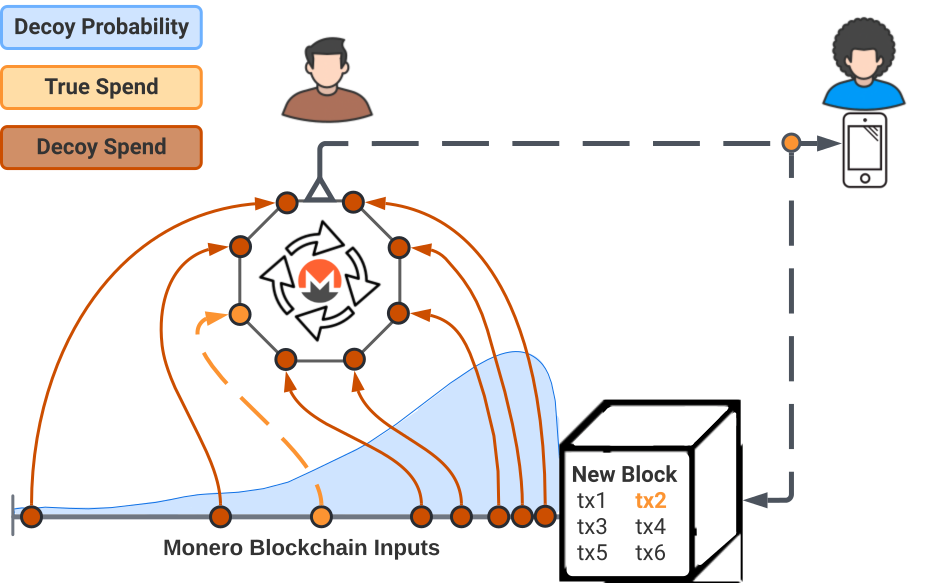
\includegraphics[scale=0.4]{images/decoy-selection-with-adequate-DSA}
\par\end{centering}
\begin{centering}
{\footnotesize{}Image designed by ACK-J (https://github.com/ack-j)}{\footnotesize\par}
\par\end{centering}
\label{figure-adequate-dsa}
\end{figure}

The height of the blue shape in Figure \ref{figure-adequate-dsa}
represents the probability that the decoy selection algorithm selects
outputs as decoys from certain blockchain time stamps. Younger outputs
are more likely to be selected as decoys since younger outputs are
also more likely to be the real spends. Since there is a high probability
that a decoy (red circle) could be selected from the same time interval
as the real spend (orange), it is difficult for an anti-privacy adversary
to deduce that the orange circle is the real spend.

Figure \ref{figure-defective-dsa} shows what would happen if the
decoy selection algorithm were severely defective. There is a portion
of the age distribution that the decoy selection algorithm will never
select from. The height of the blue shape is zero at that interval.
In this hypothetical, the fact that no decoy would be selected in
that interval would be known by an anti-privacy adversary since the
decoy selection algorithm is written into Monero's public open source
code, at least for Monero wallets that are open source. Therefore,
there would be a 100 percent probability that the ring member selected
in that interval was the real spend. This particular transaction would
be 100 percent traceable. To repeat, this is the extreme case that
does not happen in practice. The current decoy selection algorithm
is not severely defective like this hypothetical example, but it has
significant shortcomings.

\begin{figure}[H]
\caption{Defective Decoy Selection Algorithm}

\begin{centering}
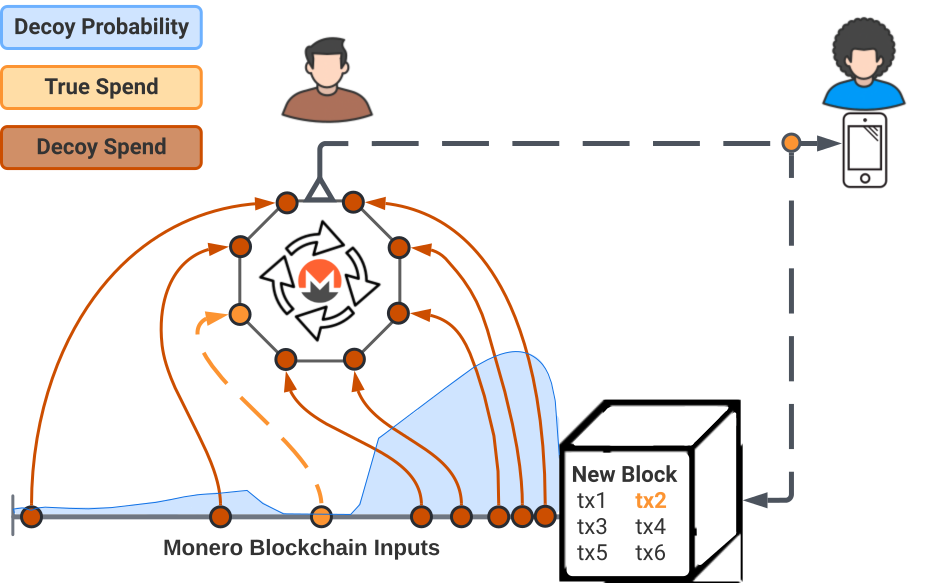
\includegraphics[scale=0.4]{images/decoy-selection-with-defective-DSA}
\par\end{centering}
\begin{centering}
{\footnotesize{}Image designed by ACK-J (https://github.com/ack-j)}{\footnotesize\par}
\par\end{centering}
\label{figure-defective-dsa}
\end{figure}

The ideal decoy selection algorithm would select decoys from every
point on the age distribution in exact proportion to the real spends.
For a ring size of 16, this ideal algorithm would provide 15 decoys
of ``camouflage'' on top of every real spend across the entire age
distribution. In ideal circumstances, such an algorithm would not
give any hint about the real spend to an anti-privacy adversary. The
best an adversary could do is random guessing about the real spend,
which would only achieve a success rate of $1/16=6.25\%$. The ``defective''
algorithm described above provided zero decoys in a certain age interval,
which would lead to full traceability of transactions that spend outputs
that were a certain age. Monero's current decoy selection algorithm
lies somewhere between the two extremes of ideal and severely defective.
The goal of OSPEAD is to move the decoy selection algorithm much closer
to the ideal shape.

\section{The Solution\label{sec:The-Solution}}

The goal of OSPEAD is to use a special type of mathematical function
called a parametric probability density function to match the real
spend age distribution as closely as possible. The close match will
provide about 15 decoys for every real spend along nearly every interval
of the age distribution. The match cannot be perfect, however. Parametric
probability density functions can only serve as an approximation of
complex real human behavior.

There are only a limited number of decoys available per ring. Therefore,
if more decoy ``camouflage'' is moved from section A to section
B on the age distribution, users who happen to spend outputs of an
age that falls into section A will experience a reduction in privacy;
users spending from section B will experience an increase in privacy.
Therefore with the imperfect parametric probability distribution functions
there is an unavoidable trade-off. The terms of the trade-off can
be made precise mathematically, but the correct choice of trade-off
is a judgment call.

Given that the ``correct'' trade-off is a judgment call, OSPEAD
involves a procedure to obtain the best decoy selection algorithm
under several different sets of criteria. Once these candidate algorithms
are determined, a single best algorithm will be selected though a
judgment call. In the next section I describe the proposed sets of
criteria: privacy impoverishment, economic welfare, inequality minimization,
worst-case-scenario minimization, Maximum Likelihood Estimation, and
maximize resistance to a specific attack.

\section{Criteria for Best Fit\label{sec:Criteria-for-Best-Fit}}

At first glance constructing $f_{D}(x)$, the probability density
function (PDF) of the decoy selection algorithm, appears to be a standard
problem: Extract the real spend age distribution $f_{S}(x)$ ``data''
through some method and then fit some distribution to it in order
to form $f_{D}(x)$. Typically in applied statistical work, ``fitting
some distribution'' would be done via nonparametric means or Maximum
Likelihood Estimation (MLE) for a parametric approach. Since we are
setting aside nonparametric methods in the short term, MLE may see
like the way forward.

I would argue instead that what we confront here is not actually a
standard problem, despite appearances. An MLE approach, which is the
approach taken in \cite{2018}, may make sense if what we are interested
in is conducting hypothesis tests on the parameters of parametric
distribution families, a typical scientific exercise. In fact, MLE
is quite good at that task, assuming certain crucial assumptions are
met, since asymptotically it is usually guaranteed to achieve minimum
variance among unbiased estimators. 

What we are trying to do here with construction of $f_{D}(x)$ has
little to do with conducting hypothesis tests, however. Most statistical
methods are interested in separating statistical signal from noise.
What we are trying to do is quite the opposite: merge the signal (real
spends) and noise (decoys) so that even a determined and sophisticated
statistician cannot distinguish them. We are not trying to minimize
variance in fitting $f_{D}(x)$ to $f_{S}(x)$. Rather, we are trying
to minimize risk to user privacy. We are trying to minimize traceability
of Monero transactions. This goal requires us to be more creative
in our approach.

In general, our goal is to ``cover'' every age interval with 15
decoys for every real spend that comes from that interval. A user
who spends from a point of the age distribution that is not covered
by at least 15 decoys experiences a privacy deficit. A user who spends
from a point of the age distribution that is covered by more than
15 decoys has a surplus of decoys. To approach the ideal of all users
being protected by a single-hop anonymity set of 16, we can move these
decoys from the surplus at particular age $x$ values to the $x$
values with deficits. I will build OSPEAD around the idea of minimizing
this privacy deficit for all $x$, defined as $h(x)=\max\left\{ 0,f_{S}(x)-f_{D}(x)\right\} $.
I also include a symmetric option: $h_{sym}(x)=\left|f_{S}(x)-f_{D}(x)\right|$
as a possible minimization objective.

To justify my proposed methodology, I will quote extensively from
the second edition of \textit{Statistical Inference} by George Casella
\& Roger L. Berger (\cite{CasellaBerger2002}). In the book's preface,
the authors write, ``The purpose of this book is to build theoretical
statistics (as different from mathematical statistics) from the first
principles of probability theory....The book is intended for first-year
graduate students majoring in statistics or in a field where a statistics
concentration is desirable.'' As far as I can tell, it is widely
used for that purpose, at least within economics. For example, the
first course in the econometrics sequence of MIT's economics doctoral
program uses the book as its primary textbook.\footnote{\href{https://ocw.mit.edu/courses/economics/14-381-statistical-method-in-economics-fall-2018/syllabus/}{https://ocw.mit.edu/courses/economics/14-381-statistical-method-in-economics-fall-2018/syllabus/}\\
Other economics doctoral programs likely do as well, but we cannot
know for sure since many of them keep their syllabi hidden behind
student login screens.} Therefore, in my view the book is authoritative enough to lean on
in justifying my proposed approach.

I will begin by quoting from pages 348--350:
\begin{quote}
\textit{7.3.4 Loss Function Optimality}

Our evaluations of point estimators have been based on their mean
squared error performance. Mean squared error is a special case of
a function called a \textit{loss function}. The study of the performance,
and the optimality, of estimators evaluated through loss functions
is a branch of \textit{decision theory}.

After the data $\mathbf{X}=\mathbf{x}$ are observed, where $\mathbf{X}\sim f(\mathbf{x}|\theta)$,
$\theta\in\Theta$, a decision regarding $\theta$ is made. The set
of allowable decisions is the \textit{action space}, denoted by $\mathcal{A}$.
Often in point estimation problems $\mathcal{A}$ is equal to $\Theta$,
the parameter space, but this will change in other problems (such
as hypothesis testing---see Section 8.3.5).

The loss function in a point estimation problem reflects the fact
that if an action $a$ is close to $\theta$, then the decision $a$
is reasonable and little loss is incurred. If $a$ is far from $\theta$,
then a large loss is incurred. The loss function is a nonnegative
function that generally increases as the distance between $a$ and
$\theta$ increases. If $\theta$ is real-valued, two commonly used
loss functions are

\[
{\textstyle absolute\:error\:loss},\quad L(\theta,a)=|a-\theta|,
\]

and

\[
{\textstyle squared\:error\:loss},\quad L(\theta,a)=(a-\theta)^{2}.
\]

Both of these loss functions increase as the distance between $\theta$
and $a$ increases, with minimum value $L(\theta,\theta)=0$. That
is, the loss is minimum if the action is correct. Squared error loss
gives relatively more penalty for large discrepancies, and absolute
error loss gives relatively more penalty for small discrepancies.
A variation of squared error loss, one that penalizes overestimation
more than underestimation, is

\begin{equation}
L(\theta,a)=\begin{cases}
(a-\theta)^{2} & \mathrm{if}\:a<\theta\\
10(a-\theta)^{2} & \mathrm{if}\:a\geq\theta.
\end{cases}\label{eq:variation-sq-error-loss}
\end{equation}

A loss that penalizes errors in estimation more if $\theta$ is near
0 than if $|\theta|$ is large, a relative squared error loss, is

\[
L(\theta,a)=\dfrac{(a-\theta)^{2}}{|\theta|+1}.
\]

Notice that both of these last variations of squared error loss could
have been based instead on absolute error loss. \textbf{In general,
the experimenter must consider the consequences of various errors
in estimation for different values of $\boldsymbol{\theta}$ and specify
a loss function that reflects these consequences.} {[}my emphasis{]}

In a loss function or \textit{decision theoretic} analysis, the quality
of an estimator is quantified in its \textit{risk function}; that
is, for an estimator $\delta(\mathbf{x})$ of $\theta$, the risk
function, a function of $\theta$, is

\begin{equation}
R(\theta,\delta)=\mathrm{E}_{\theta}L(\theta,\delta(\mathbf{X})).\label{eq:risk-function-general}
\end{equation}

At a given $\theta$, the risk function is the average loss that will
be incurred if the estimator $\delta(\mathbf{x})$ is used.

Since the true value of $\theta$ is unknown, we would like to use
an estimator that has a small value of $R(\theta,\delta)$ for all
values of $\theta$. This would mean that, regardless of the true
value of $\theta$, the estimator will have a small expected loss.
If the qualities of two different estimators, $\delta_{1}$ and $\delta_{2}$,
are to be compared, then they will be compared by comparing their
risk functions, $R(\theta,\delta_{1})$ and $R(\theta,\delta_{2})$.
If $R(\theta,\delta_{1})<R(\theta,\delta_{2})$ for all $\theta\in\Theta$,
then $\delta_{1}$ is the preferred estimator because $\delta_{1}$
performs better for all $\theta$. More typically, the two risk functions
will cross. Then the judgment as to which estimator is better may
not be so clear-cut.

The risk function for an estimator $\delta$ is the expected loss,
as defined in (\ref{eq:risk-function-general}). For squared error
loss, the risk function is a familiar quantity, the mean squared error
(MSE) that was used in Section 7.3.1. There the MSE of an estimator
was defined as $\mathrm{MSE}(\theta)=\mathrm{E}_{\theta}(\delta(\mathbf{X})-\theta)^{2}$,
which is just $\mathrm{E}_{\theta}L(\theta,\delta(\mathbf{X}))=R(\theta,\delta)$
if $L(\theta,a)=(a-\theta)^{2}$. As in Chapter 7 we have that, for
squared error loss,

\[
R(\theta,\delta)=\mathrm{Var}_{\theta}\,\delta(\mathbf{X})+(\mathrm{E}_{\theta}\delta(\mathbf{X})-\theta)^{2}=\mathrm{Var}_{\theta}\,\delta(\mathbf{X})+(\mathrm{Bias}_{\theta}\,\delta(\mathbf{X}))^{2}.
\]

This risk function for squared error loss clearly indicates that a
good estimator should have both a small variance and a small bias.
A decision theoretic analysis would judge how well an estimator succeeded
in simultaneously minimizing these two quantities.

\textbf{It would be an atypical decision theoretic analysis in which
the set $\boldsymbol{\mathcal{D}}$ of allowable estimators was restricted
to the set of unbiased estimators, as was done in Section 7.3.2.}
{[}my emphasis{]} Then, minimizing the risk would just be minimizing
the variance. A decision theoretic analysis would be more comprehensive
in that both the variance and bias are in the risk and will be considered
simultaneously. An estimator would be judged good if it had a small,
but probably nonzero, bias combined with a small variance.
\end{quote}
The text then goes into several specific examples of risk analysis
and then briefly explores risk within a Bayesian framework. What does
Section 7.3.2 (page 334), referenced above, say?
\begin{quote}
\textit{7.3.2 Best Unbiased Estimators}

As noted in the previous section, a comparison of estimators based
on MSE considerations may not yield a clear favorite. Indeed, there
is no one ``best MSE'' estimator. Many find this troublesome or
annoying, and rather than doing MSE comparisons of candidate estimators,
they would rather have a ``recommended'' one.

The reason that there is no one ``best MSE'' estimator is that the
class of all estimators is too large a class. (For example, the estimator
$\hat{\theta}=17$ cannot be beaten in MSE at $\theta=17$ but is
a terrible estimator otherwise.) One way to make the problem of finding
a ``best'' estimator tractable is to limit the class of estimators.
A popular way of restricting the class of estimators, the one we consider
in this section, is to consider only unbiased estimators.

If $W_{1}$ and $W_{2}$ are both unbiased estimators of a parameter
$\theta$, that is, $\mathrm{E}_{\theta}W_{1}=\mathrm{E}_{\theta}W_{2}=\theta$,
then their mean squared error are equal to their variances, so we
should choose the estimator with the smaller variance. If we can find
an unbiased estimator with uniformly smallest variance---a best unbiased
estimator---then our task is done.
\end{quote}
\cite{CasellaBerger2002} then go on to give a formal definition of
best unbiased estimator --- also known as uniform minimum variance
unbiased estimator (UMVUE) --- in Definition 7.3.7 and then give
the Cram{\'e}r--Rao Lower Bound (CRLB) in Theorem 7.3.9 and Corollary
7.3.10. Corollary 7.3.15 is also useful. The gist of the discussion
is that certain unbiased estimators of a parameter $\theta$ (the
text uses the notation $\tau(\theta)$, with $\tau$ being some continuous
function of $\theta$, in order to be more general) of a distribution
$f(\mathbf{x}|\theta)$ may achieve the lowest variance possible in
this setting: the Cram{\'e}r--Rao Lower Bound (CRLB).

Now I will move on to examining Maximum Likelihood Estimation (MLE)
in this entire context. First I will reference the definition of asymptotic
variance from \cite{CasellaBerger2002}, page 471. Let $k_{n}$ be
some normalizing constant.
\begin{quote}
\textbf{Definition 10.1.9}$\quad$For an estimator $T_{n}$, suppose
that $k_{n}(T_{n}-\tau(\theta))\rightarrow n(0,\sigma^{2})$ in distribution.
The parameter $\sigma^{2}$ is called the \textit{asymptotic variance}
or \textit{variance of the limit distribution} of $T_{n}$.
\end{quote}
I also need their definition of asymptotic efficiency to make my point:
\begin{quote}
\textbf{Definition 10.1.11}$\quad$A sequence of estimators $W_{n}$
is asymptotically efficient for a parameter $\tau(\theta)$ if $\sqrt{n}\left[W_{n}-\tau(\theta)\right]\rightarrow n\left[0,v(\theta)\right]$
in distribution and

\[
v(\theta)=\dfrac{\left[\tau'(\theta)\right]^{2}}{\mathrm{E}_{\theta}\left(\left(\frac{\partial}{\partial\theta}\log f\left(X|\theta\right)\right)^{2}\right)};
\]

that is, the asymptotic variance of $W_{n}$ achieves the Cram{\'e}r--Rao
Lower Bound.
\end{quote}
Finally, we come to one of the primary reasons MLE is so popular in
applied statistical work:
\begin{quote}
\textbf{Theorem 10.1.12 (Asymptotic efficiency of MLEs)}$\quad$Let
$X_{1},X_{2},....,$ be iid $f(x|\theta)$, let $\hat{\theta}$ denote
the MLE of $\theta$, and let $\tau(\theta)$ be a continuous function
of $\theta$. Under the regularity conditions in Miscellanea 10.6.2
on $f(x|\theta)$ and, hence $L(\theta,\mathbf{x})$ {[}this expression,
the likelihood function, is defined in Theorem 10.1.6 as $L(\theta|\mathbf{x})=\prod_{i=1}^{n}f(x_{i}|\theta)$
{]}, 

\[
\sqrt{n}\left[\tau(\hat{\theta})-\tau(\theta)\right]\rightarrow n\left[0,v(\theta)\right],
\]

where $v(\theta)$ is the Cram{\'e}r--Rao Lower Bound. That is, $\tau(\hat{\theta})$
is a consistent and asymptotically efficient estimator of $\tau(\theta)$.
\end{quote}
Later, at the top of page 477, \cite{CasellaBerger2002} make this
comment:
\begin{quote}
Since the MLE is typically asymptotically efficient, another estimator
cannot hope to beat its asymptotic variance. However, other estimators
may have other desirable properties (ease of calculation, \textbf{robustness
to underlying assumptions} {[}my emphasis{]}) that make them desirable.
In such situations, the efficiency of the MLE becomes important in
calibrating what we are giving up if we use an alternative estimator.
\end{quote}
\par\noindent\rule{\textwidth}{0.4pt}\\

Let us break down what \cite{CasellaBerger2002} are saying in these
passages, and how they relate to OSPEAD. They set up a framework for
decision-making based on statistical analysis. Loss functions, decision
theory, and risk functions are the main elements of this framework.
They then discuss some of the most common loss functions, Mean Squared
Error (MSE) being one of them. I note in passing that they discuss
a ``variation'' on MSE in equation (\ref{eq:variation-sq-error-loss})
that bears some resemblance to my privacy deficit notion, defined
as $h(x)=\max\left\{ 0,f_{S}(x)-f_{D}(x)\right\} $, in that it is
asymmetric in penalization of under- and over-estimation of some quantity.

Minimizing MSE for estimates of a particular parameter $\theta$ is
a fair goal for statistical analyses whose purpose is to conduct traditional
hypothesis tests regarding the true value of $\theta$ in line with
the Popperian falsification paradigm of science. Lower MSE generally
would lead to higher statistical power and therefore greater ability
to avoid Type II error in hypothesis tests. \cite{CasellaBerger2002}
write, ``In general, the experimenter must consider the consequences
of various errors in estimation for different values of $\theta$
and specify a loss function that reflects these consequences.'' By
minimizing bias and variance explicitly, MSE --- as a loss function
--- performs well in avoiding the Type I and Type II error consequences
in null hypothesis testing and therefore MSE often makes sense to
use as a loss function in scientific hypothesis testing.

\cite{CasellaBerger2002} go further and observe, ``It would be an
atypical decision theoretic analysis in which the set $\mathcal{D}$
of allowable estimators was restricted to the set of unbiased estimators,
as was done in Section 7.3.2.'' As I highlighted, MLE typically has
lowest variance, asymptotically, among estimators with zero bias.
Therefore, restricting ourselves to MLE in tackling the problem before
us --- construction of the PDF for the decoy selection algorithm
--- would likely seem ill-advised to \cite{CasellaBerger2002}, since
the class of unbiased estimators might not be suitable.

Note also that maximum likelihood estimators are point estimators
for the particular $\theta$ parameters of PDFs. In theory, the estimated
$\hat{\theta}$ will yield the corresponding theoretical distributions
that fit the target empirical distributions well, although only under
the assumption that the empirical distribution being fitted exactly
equals the chosen theoretical PDF. There is no guarantee that variance
--- or bias for that matter --- for the distribution itself will
be small when using MLE to fit the wrong theoretical PDF to an empirical
distribution. Given the fact that we are interested in the whole distributions
themselves, i.e. $f_{S}(x)$ and $f_{D}(x)$, and not just parameters
of parametric distributions, the justification for using MLE in this
setting is even weaker. In just a moment I will convert the problem
of fitting distributions into a parametric one, so that the true problem
is better illustrated.

\par\noindent\rule{\textwidth}{0.4pt}\\

Until now I have dealt with $f_{S}(x)$ and $f_{D}(x)$ as if they
were probability density functions, i.e. as if the domain of the functions
were continuous. However, in reality they are probability mass functions,
i.e. the domain of the functions are discrete. The real spend age
distributions are only meaningful in terms of the discrete blocks
on the blockchain, since miners can arrange valid transactions within
a block in any order they choose. We can leverage this fact for the
following analysis.

Define a set of parameters $\boldsymbol{\theta}$ as follows:

\[
\boldsymbol{\theta}=\left\{ \theta_{1},\theta_{2},...,\theta_{N}\right\} =\left\{ f_{S}(1),f_{S}(2),...,f_{S}(N)\right\} 
\]

So $\theta_{1}$ is the value of $f_{S}(x)$ when $x=1$, i.e. the
first-available block that an output can be spent in. $\theta_{N}$
refers to the first block where RingCT outputs appeared. My definition
here is not completely rigorous, since the blockchain is lengthening
constantly, and therefore the number of elements of $\boldsymbol{\theta}$
is increasing by the hour.

What we wish to estimate is $\boldsymbol{\theta}$ --- every element
of it. Or, more specifically, we wish to construct some $f_{D}(x)$
such that $f_{D}(x_{i})$ is ``close'' --- in some sense to be
defined shortly --- to each $\theta_{i}$, for every $i$. With a
nonparametric approach, we may be able to tackle each element $\theta_{i}$
individually, more or less. With a parametric approach, we cannot
hope to do so. Therefore, we must establish some overall metric, or
metrics, of ``success''. In other words, we must define and justify
a set $\mathcal{L}$ of loss functions. This is our first task. Our
second task is to define a set $\mathcal{D}$ of allowable estimators.

In equation (\ref{eq:risk-function-general}), \cite{CasellaBerger2002}
defined the risk function as $R(\theta,\delta)=\mathrm{E}_{\theta}L(\theta,\delta(\mathbf{X}))$.
For the time being, we will assume that $\boldsymbol{\theta}$ is
deterministic and therefore the risk function equals the loss function.
The $\boldsymbol{\theta}$ is actually stochastic --- it changes
over time as user spending patterns change over time --- which will
be dealt with in \textbf{Section \ref{sec:Dynamic-Risk-and-Forecasting}
Dynamic Risk and Forecasting}.

There are some similarities between the Differential Privacy framework
and Monero's ring signature privacy model. Differential Privacy seeks
a balance between the desire to perform statistical analysis on private
data and the need to protect individuals from discovery of their private
information. Monero seeks to maximize privacy of users, but is constrained
by reasonable limits on ring size. I looked through the Differential
Privacy literature for some criteria for fitting a decoy selection
algorithm. In general there are utility-based criteria for resolving
the balance between statistical analysis and user privacy for each
user, but there is not yet a way to resolve our problem(\cite{Hsu2014}).
Our problem is different in that a particular ring size is fixed,
and then trade-offs \textit{between users} need to be determined. 

In ``Research Roadmap for an Overhaul of Monero's Mixin Selection
Algorithm'', which I submitted to Monero's Vulnerability Response
Process in 2021, I wrote:
\begin{quote}
How do we construct $f_{M}(x)$ {[}the decoy selection algorithm{]}
for best overall privacy if we restrict ourselves to parametric distributions,
and therefore cannot achieve $f_{S}(x)\approx f_{M}(x)$ for all values
of $x$? Well, it depend {[}sic{]} on how we define ``best''. Below
are six approaches. I have the mathematical definitions of these worked
out in my head, but they are not written here:

$\vphantom{}$

1) Privacy impoverishment

2) Economic welfare

3) Inequality minimization

4) Worst-case-scenario minimization

5) Maximum Likelihood Estimation

6) Maximize resistance to a specific attack

$\vphantom{}$

Now that a set of objective functions have been defined, one could
imagine optimizing these objective functions in a numerical optimization
procedure where each parametric distribution family with support of
$[0,\infty)$ is permuted over 1-6 above.
\end{quote}
These objective functions are the loss functions in the framework
of \cite{CasellaBerger2002}. Many of them are forms of minimum divergence
estimators (\cite{Maji2019}). Just two more bits of housekeeping
before I can mathematically define these 1-6 loss functions. First,
to be consistent with the notation of \cite{CasellaBerger2002}, define
$f_{D}(x_{i})\equiv a_{i}$.

Second, we must think about how to give weight to each $\theta_{i}$.
Do we give equal weight to every $\theta_{i}$? That would mean that
outputs years old would be given the same importance as outputs just
a few minutes or hours old. Weighting the loss function by the value
of $\theta_{i}$ seems more reasonable since that would, in effect,
give each spent output equal importance. However, we are trying to
protect the privacy of people, not outputs. 

Say that User A re-spends outputs frequently, and so has real spends
that are in the thick portion of $f_{S}(x)$. Say that User B re-spends
outputs infrequently, and therefore has real spends that are in the
thin portion of $f_{S}(x)$. Furthermore, User A would be able to
generate more transactions than User B simply because of rapidly re-spending
outputs. Therefore, only weighting the loss function by the value
of $\theta_{i}$ would (maybe unfairly) give more importance to User
A than User B, just due to the way that the mathematics work out.
The way forward is not exactly clear. I think it could make sense
to try several intermediate weighting schemes.

First, my recommendation is to only give weight to elements of $\boldsymbol{\theta}$
when there is a privacy deficit, i.e. when $h(x)=\max\left\{ 0,f_{S}(x)-f_{D}(x)\right\} $
is nonzero. Later we will use $\boldsymbol{1}\{x\}$, the indicator
function, for this part of the weighting scheme, or the $\min\left\{ x\right\} $
operator, depending on the context.\footnote{\href{https://en.wikipedia.org/wiki/Indicator_function}{https://en.wikipedia.org/wiki/Indicator\_function}}
For comparison purposes, I will also include the symmetric counterpart
$h_{sym}(x)=\left|f_{S}(x)-f_{D}(x)\right|$ that seeks to avoid privacy
surpluses as much as it seeks to avoid privacy deficits. To allow
for multiple intermediate weighting schemes, define this weight function: 

\begin{equation}
w(\theta_{i},\lambda)=\lambda\theta_{i}+(1-\lambda)\tfrac{1}{N}\label{eq:weight-fn}
\end{equation}

Thus, when $\lambda=1$, $w(\theta_{i},\lambda)$ is fully weighted
by the value of $\theta_{i}$. When $\lambda=0$, $w(\theta_{i},\lambda)$
gives equal weight to each $\theta_{i}$. Tentatively, let $\boldsymbol{\lambda}=\left\{ 0,0.5,0.9,0.95,0.99,0.999,0.9999,1\right\} $.

Now we are ready to define the set $\mathcal{L}$ of loss functions.

\subsection{Privacy impoverishment}

To me, the privacy deficit formulation is somewhat reminiscent of
a poverty line. Below a certain defined threshold individuals are
considered to be impoverished. In the case of a standard poverty indicator,
there is some poverty line $z$ defined by a researcher or government
entity. In the case of Monero user privacy, the corresponding ``poverty
line'' would be $f_{S}(x)$, which is different for every $x$.

The Foster--Greer--Thorbecke (FGT) indices are a family of widely-used
poverty indicators. They are defined as

\[
FGT_{\alpha}=\frac{1}{N}\sum_{i=1}^{H}\left(\dfrac{z-y_{i}}{z}\right)^{\alpha}
\]

where $N$ is the number of people in the population under study,
$H$ is the number of people within that population who are below
the poverty line, $z$ is the poverty line, $y_{i}$ is the income
(or consumption) of each individual $i$ who is under the poverty
line, and $\alpha$ is a parameter that controls weighting. 

If $\alpha$ is high, then people far below the poverty line are given
much more weight than people just barely below the poverty line. When
$\alpha=0$, $FGT_{0}$ is simply the poverty headcount. When $\alpha=1$,
$FGT_{1}$ is the poverty gap index. When $\alpha=2$, $FGT_{2}$
weights each person's poverty gap by its square, and for $\alpha=3$,
by its cube, and so forth.

A loss function analogue can be defined:

\begin{equation}
L_{FGT_{\alpha}}(\boldsymbol{\theta},\boldsymbol{a},\lambda)=\dfrac{1}{N}\stackrel[i=1]{N}{\sum}\boldsymbol{1}\left\{ a_{i}<\theta_{i}\right\} w(\theta_{i},\lambda)\left(\dfrac{\theta_{i}-a_{i}}{\theta_{i}}\right)^{\alpha}\label{eq:L-FGT}
\end{equation}

The $\boldsymbol{1}\left\{ a_{i}<\theta_{i}\right\} $ indicator function
ensures that $a_{i}$'s are only counted when there is some privacy
deficit. The symmetric counterpart $L_{FGT_{\alpha},sym}(\boldsymbol{\theta},\boldsymbol{a},\lambda)$
would omit the $\boldsymbol{1}\left\{ a_{i}<\theta_{i}\right\} $
term and replace $\left(\dfrac{\theta_{i}-a_{i}}{\theta_{i}}\right)^{\alpha}$with
$\left(\left|\dfrac{\theta_{i}-a_{i}}{\theta_{i}}\right|\right)^{\alpha}$.
Using $\alpha=0$ probably doesn't make sense for our purposes. Using
$\boldsymbol{\alpha}=\{1,2,3\}$ is reasonable. 

\subsection{Economic welfare}

A full discussion of the meaning and theory of economic welfare is
outside of the scope of this document. The basic idea is that people
are theorized to have preferences that can be approximated via a mathematical
function. These approximating functions are called utility functions.
When people's preferences are satisfied, they obtain utility. When
the preferences are satisfied to a higher degree, they obtain higher
utility. In essence, when an individual's utility is higher, their
happiness is higher. Within the framework of neoclassical economics,
individuals strive to maximize their utility, subject to the constraints
they encounter in the world. The analysis of aggregate population-level
utility is the realm of welfare economics.

We may assume that Monero users prefer to have privacy and therefore
some ``privacy utility function'' in this specific context could
be defined. In practice, the loss function derived from this type
of analysis will look similar to the $L_{FGT_{\alpha}}(\boldsymbol{\theta},\boldsymbol{a},\lambda)$
privacy impoverishment loss function, but with a different interpretation.

There are dozens of utility functions to choose from. One of the more
appropriate ones in the present context is the Constant Relative Risk
Aversion (CRRA) utility function:

\begin{equation}
u_{CRRA_{\eta}}(y)=\begin{cases}
\frac{y^{1-\eta}}{1-\eta} & \eta\geq0,\eta\neq1\\
\ln(y) & \eta=1
\end{cases}
\end{equation}

where $\eta$ is the coefficient of constant relative risk aversion.
The CRRA utility function makes sense to use in this context because
(1) At a basic level, it takes a single argument, unlike other classes
of utility functions that deal with multiple goods and services; (2)
It explicitly deals with risk; (3) It has an adjustable parameter
$\eta$ that we can use to explore the sensitivity of the results;
(4) For $\eta\geq1$, the CRRA utility function approaches $-\infty$
as $y$ approaches zero. 

The (4) characteristic serves as an important advantage compared to
the privacy impoverishment framework since in theory the $L_{FGT_{\alpha}}(\boldsymbol{\theta},\boldsymbol{a},\lambda)$
loss function would allow $f_{D}(x)$ to have zero mass at some $x$
values --- and therefore any ring members having an age corresponding
to those $x$ values would be clearly identifiable as real spends.
In addition, a numerical optimization process that used the CRRA utility
function as its basis would avoid at all costs $f_{D}(x)=0$ for any
and all $x$ values as long as $\eta$ is chosen so that $\eta\geq1$.

In a welfare economics framework, generally some discussion of the
Pareto weights and Pareto efficiency would be appropriate. However,
that type of discussion has little practical effect on the analysis
here and it would generally only be of interest to economists, so
I will elide it here.

Now we are ready to define an economic welfare loss function:

\begin{equation}
L_{Welfare_{\eta}}(\boldsymbol{\theta},\boldsymbol{a},\lambda)=\left(-1\right)\dfrac{1}{N}\stackrel[i=1]{N}{\sum}w(\theta_{i},\lambda)\left(u_{CRRA_{\eta}}\left(\min\left\{ \tfrac{a_{i}}{\theta_{i}},1\right\} \right)\right)\label{eq:L-Welfare}
\end{equation}

The $(-1)$ scalar is to make this a \textit{loss} function to be
minimized. As is typical, the CRRA utility function increases with
its argument, and privacy increases as $a_{i}$ becomes closer to
$\theta_{i}$, i.e. as $f_{D}(i)$ becomes closer to $f_{S}(i)$.
We use the $\min\left\{ x\right\} $ operator here. When $a_{i}<\theta_{i}$,
the utility function is applied to $\tfrac{a_{i}}{\theta_{i}}$. When
$a_{i}\geq\theta_{i}$, the utility function is applied to one, as
if $a_{i}=\theta_{i}$, since users spending outputs from this block
$i$ suffer no privacy deficit as I have defined it. The symmetric
counterpart $L_{Welfare_{\eta},sym}(\boldsymbol{\theta},\boldsymbol{a},\lambda)$
would replace $\min\left\{ \tfrac{a_{i}}{\theta_{i}},1\right\} $
with $\tfrac{a_{i}}{\theta_{i}}$.

The choice for $\eta$ is somewhat open-ended. Perhaps five values
should be tested, to get some sense of the sensitivity of the results
to the choice of $\eta$. One of the values should be $\eta=1$ so
that log utility is used. It is less clear what the remaining four
values should be. Some experimentally-determined values for $\eta$
for the utility of income are available in the literature, but how
individuals' utility functions for income and privacy relate to one
another is unclear. Tentatively, let us set $\boldsymbol{\eta}$ to
$\boldsymbol{\eta}=\left\{ 0.5,1,2,5\right\} $. 

\subsection{Inequality minimization}

Another possible loss function is an inequality metric. The privacy
impoverishment and economic welfare frameworks dealt with the absolute
privacy of each user. We may also want to consider a framework that
explicitly compares users to each other, in terms of the privacy that
a $f_{D}(x)$ provides. A loss function that attempts to minimize
inequality of privacy among users may be appropriate.

One of the most widely-used inequality metrics is the Gini coefficient
(or Gini index). The Gini coefficient has many attractive theoretical
properties that I will not recite here. Its main drawback is that
its value is not very interpretable for laypeople. (The most intuitive
explanation involves the Lorenz curve.) Given that we are already
far into the realm of difficulty with interpretation of these loss
functions, the low interpretability of the Gini coefficient should
not stop us from using it.

One formulation of the Gini coefficient is:

\[
G(\mathbf{x})=\dfrac{\stackrel[i=1]{n}{\sum}\stackrel[j=1]{n}{\sum}\left|x_{i}-x_{j}\right|}{2\stackrel[i=1]{n}{\sum}\stackrel[j=1]{n}{\sum}x_{j}}=\dfrac{\stackrel[i=1]{n}{\sum}\stackrel[j=1]{n}{\sum}\left|x_{i}-x_{j}\right|}{2n^{2}\bar{x}}
\]

This formulation is somewhat easy to interpret, although it is computationally
expensive as it requires about $\left(n^{2}-n\right)/2$ arithmetic
operations. It does not contemplate weights, so it must be modified.
\cite{Creedy2015} provides some guidance.

First, the formula suggested by Creedy requires that the weights sum
up to $n$, i.e. $\sum_{i=1}^{n}w_{i}=n$. The weights that we will
use, $w(\theta_{i},\lambda)$ could easily be normalized to ensure
$\sum_{i=1}^{n}w(\theta_{i},\lambda)=n$.

In his equation (17), Creedy suggests the following weighted formula:

\[
G(\mathbf{x})=\dfrac{\stackrel[i=1]{n}{\sum}\stackrel[j=i+1]{n}{\sum}w_{i}w_{j}\left|x_{i}-x_{j}\right|}{\stackrel[i=1]{n}{\sum}w_{i}\stackrel[i=1]{n}{\sum}w_{i}x_{i}}
\]

If we let $x_{i}$ be $\tfrac{a_{i}}{\theta_{i}}$ as with the economic
welfare loss function, the corresponding loss function for our problem
would then be:

\begin{equation}
\begin{array}{c}
L_{Gini}(\boldsymbol{\theta},\boldsymbol{a},\lambda)=\dfrac{\stackrel[i=1]{n}{\sum}\stackrel[j=i+1]{n}{\sum}w(\theta_{i},\lambda)\cdot w(\theta_{j},a_{j},\lambda)\cdot\left|\min\left\{ \tfrac{a_{i}}{\theta_{i}},1\right\} -\min\left\{ \tfrac{a_{j}}{\theta_{j}},1\right\} \right|}{\stackrel[i=1]{n}{\sum}w(\theta_{i},\lambda)\stackrel[i=1]{n}{\sum}w(\theta_{i},\lambda)\cdot\min\left\{ \tfrac{a_{i}}{\theta_{i}},1\right\} }\\
\\
\mathrm{subject\:to}\quad\sum_{i=1}^{n}w(\theta_{i},\lambda)=n
\end{array}\label{eq:L-Gini}
\end{equation}

Note that the formula given in equation (17) in \cite{Creedy2015}
is just one possible way to deal with weighting to compute a Gini
coefficient. The reason that there are multiple ways to do weighting
is that weighting attempts to, in essence, interpolate parts of the
Lorenz curve. How to do that interpolation is up for debate. In his
equation (12), \cite{Creedy2015} also gives a weighted Gini formula
that is less computationally expensive. However, it would require
conversion of $w(\theta_{i},\lambda)$ to integers, which is feasible
but adds another layer of complication. The symmetric counterpart
$L_{Gini,sym}(\boldsymbol{\theta},\boldsymbol{a},\lambda)$ would
replace $\min\left\{ \tfrac{a_{i}}{\theta_{i}},1\right\} $ with $\tfrac{a_{i}}{\theta_{i}}$.

\subsection{Worst-case-scenario minimization}

Worst-case-scenario minimization is inspired by Appendix F: Minimum
Untraceability in \cite{2018}. They define $\mathrm{Ge}{}_{min}$,
the minimum possible guessing entropy of the untraceability of a transaction
input:

\begin{equation}
\mathrm{Ge}{}_{min}=\dfrac{\tfrac{1}{2}m(m+1)}{\frac{r_{max}}{r_{min}}+m}\label{eq:Ge_min_orig}
\end{equation}

where $m$ is the number of ring members and

\[
r_{max}=\underset{\forall x}{\max}\left(\dfrac{f_{S}(x)}{f_{D}(x)}\right),r_{min}=\underset{\forall x}{\min}\left(\dfrac{f_{S}(x)}{f_{D}(x)}\right)
\]

Since $m$ is a constant, and optimization procedures are insensitive
to constants, for the purposes of constructing a loss function, $\mathrm{Ge}{}_{min}$
can be simplified to 

\begin{equation}
\mathrm{Ge}{}_{min\:(optimizer)}=\frac{r_{max}}{r_{min}}\label{eq:Ge_min_optimizer}
\end{equation}

The logic to construct $\mathrm{Ge}{}_{min\:(optimizer)}$ is as follows:

\[
\begin{array}{ccccc}
\mathrm{Ge}{}_{min\:(optimizer)} & = & \dfrac{\tfrac{1}{2}m(m+1)}{\tfrac{r_{max}}{r_{min}}+m}\\
\\
 & \propto & \dfrac{1}{\tfrac{r_{max}}{r_{min}}+m} &  & \textrm{scaling by \ensuremath{\left(\tfrac{1}{2}m(m+1\right)^{-1}} is a monotonic transformation}\\
\\
 & \cong & \tfrac{r_{max}}{r_{min}}+m &  & g(x)=\frac{1}{x}\textrm{ is a strictly decreasing monotonic transformation}\\
\\
 & \cong & \tfrac{r_{max}}{r_{min}} &  & \textrm{subtracting m is a monotonic transformation}
\end{array}
\]

(I am using the $\cong$ symbol loosely here.) Therefore, a $f_{D}(x)$
that minimizes (\ref{eq:Ge_min_optimizer}) will also maximize (\ref{eq:Ge_min_orig})

$ $

Putting these ideas into the loss function notation that I have been
using, i.e.

\[
r_{max}=\underset{\forall i}{\max}\left(\tfrac{\theta_{i}}{a_{i}}\right),r_{min}=\underset{\forall i}{\min}\left(\tfrac{\theta_{i}}{a_{i}}\right)
\]

gives us

\begin{equation}
L_{Worst\:case}(\boldsymbol{\theta},\boldsymbol{a})=\dfrac{\underset{i\in\left\{ 1,...,N\right\} }{\max}\left(\tfrac{\theta_{i}}{a_{i}}\right)}{\underset{i\in\left\{ 1,...,N\right\} }{\min}\left(\tfrac{\theta_{i}}{a_{i}}\right)}\label{eq:L-Worst-case}
\end{equation}

It is not clear to me how weighting by $w(\theta_{i},\lambda)$ might
work here since the numerator and denominator are both single numbers.
For the time being I will leave it out.

Although I include $L_{Worst\:case}$ in the proposed set $\mathcal{L}$
of loss functions, I am skeptical of its usefulness. It is not clear
to me that we should care about the minimum $\theta_{i}$ and $a_{i}$
among literally hundreds of thousands of them. Maybe the tail should
not wag the dog. However, it could serve as a useful comparison to
other approaches, so I include it in $\mathcal{L}$. Another issue
is that I suspect that $L_{Worst\:case}$ will not be a well-behaved
function for the purposes of numerical optimization. Given the $\min$
and $\max$ operators and how they are used here, I foresee that $L_{Worst\:case}$
as a function will have some significant discontinuities with respect
to $i$. 

\subsection{Maximum Likelihood Estimation}

As I have stated, I do not favor a MLE approach here. However, including
it in the set of loss functions $\mathcal{L}$ might serve as a useful
comparison.

Let $\boldsymbol{\beta}=\left\{ \beta_{1},...,\beta_{k}\right\} $
be the set of parameters of some parametric probability density function
$g(x|\boldsymbol{\beta})$. Then the likelihood function for some
sample $\mathbf{x}$ is

\[
L\left(\boldsymbol{\beta}|\mathbf{x}\right)=\stackrel[i=1]{n}{\prod}g\left(x_{i}|\boldsymbol{\beta}\right)
\]

To put MLE in a loss function framework, convert it into a minimization
problem and take the log to ease the computational burden:

\begin{equation}
L_{MLE}\left(\boldsymbol{\beta}|\mathbf{x}\right)=\left(-1\right)\cdot\stackrel[i=1]{n}{\sum}\log g\left(x_{i}|\boldsymbol{\beta}\right)\label{eq:L-MLE}
\end{equation}


\subsection{Maximize Resistance to an Attack\label{subsec:Maximize-Resistance-to-an-Attack}}

Define the potency of an attack on the untraceability of Monero transactions
for a specified $f_{D}(x)$ as $\mathscr{P}\left(f_{D}(x)\right)$,
the unconditional probability of correctly guessing the real spend.
Then the corresponding loss function can be defined as

\begin{equation}
L_{Attack}\left(f_{D}(x)\right)=\mathscr{P}\left(f_{D}(x)\right)\label{eq:L-Attack}
\end{equation}

\par\noindent\rule{\textwidth}{0.4pt}\\

Now that the set $\mathcal{L}$ of loss functions has been defined,
the set $\mathcal{D}$ of allowable estimators will be defined. Continuing
with the $\theta_{i}$ notation, the allowable estimators will be
selected from the set of parametric probability density functions
(PDF) $f\left(x|\boldsymbol{\beta}\right)$ such that each $\theta_{i}$
shall be estimated by the image of $i$ under $f\left(x|\boldsymbol{\beta}\right)$.
In other words, $\hat{\theta}_{i}=f\left(i|\boldsymbol{\beta}\right)$
for all $i$.

Strictly speaking, the estimator here is the minimizer of a specified
loss function in the set $\mathcal{L}$ where $a_{i}=f(i)$ for all
$i$ for some specified parametric PDF $f\left(x|\boldsymbol{\beta}\right)$.
The set of all PDFs (and probability mass functions (PMFs), for that
matter) can be all PDFs whose support is the set $[0,\infty)$. The
Wikipedia page on probability distributions lists over 40 distributions
that have such a support.\footnote{\href{https://en.wikipedia.org/wiki/List_of_probability_distributions\#Supported_on_semi-infinite_intervals,_usually_[0,\%E2\%88\%9E)}{https://en.wikipedia.org/wiki/List\_of\_probability\_distributions\#Supported\_on\_semi-infinite\_intervals,\_usually\_[0,\%E2\%88\%9E)}}
So let us say that the target number of elements of the set of PDFs
used in estimation is 40. Note that many distributions are special
cases of more general distributions and therefore the actual number
of distributions to fit may be lower than 40 in practice. Define the
set $\mathcal{F}$ of these PDFs. Let $\mathcal{B}$ be the set of
parameters of each $f\left(x|\boldsymbol{\beta}\right)$ under consideration.

\subsection{Formalized Optimization Criteria}

First, assume we have a good estimate of $f_{S}(x)$. Then OSPEAD
is the set of procedures that perform the following minimizations:

\begin{equation}
\begin{array}{ll}
\forall L\in\mathcal{L}, & \textrm{Loss functions}\\
\forall f(x|\boldsymbol{\beta})\in\mathcal{F}, & \textrm{Parametric distributions}\\
\forall\lambda\in\boldsymbol{\lambda}, & \textrm{Weight parameters for }w(\theta_{i},\lambda)\\
\forall\alpha\in\boldsymbol{\alpha}, & \textrm{Exponents for FGT poverty indicator}\\
\forall\eta\in\boldsymbol{\eta}, & \textrm{Parameters for CRRA utility}\\
\\
\underset{\boldsymbol{\beta}\in\mathcal{B}}{\min}\:L\left(f\left(x|\boldsymbol{\beta}\right)\right) & \textrm{Numerical optimization problems}\\
\\
\textrm{where}\\
\mathcal{L}=\{L_{FGT_{\alpha}},L_{Welfare_{\eta}},L_{Gini},L_{Worst\:case},L_{MLE},L_{Attack}\} & \textrm{Equations (\ref{eq:L-FGT}), (\ref{eq:L-Welfare}), (\ref{eq:L-Gini}), (\ref{eq:L-Worst-case}), (\ref{eq:L-MLE}), (\ref{eq:L-Attack})}\\
\mathcal{F}=\left\{ \textrm{Roughly 40 PDF/PMFs that have support [0,\ensuremath{\infty})}\right\} \\
\boldsymbol{\lambda}=\left\{ 0,0.5,0.9,0.95,0.99,0.999,0.9999,1\right\} \\
\boldsymbol{\alpha}=\left\{ 1,2,3\right\} \\
\boldsymbol{\eta}=\left\{ 0.5,1,5,10,50\right\} \\
\mathcal{B}=\left\{ \textrm{Sets of parameters associated with each element of }\mathcal{F}\right\} 
\end{array}\label{eq:OSPEAD}
\end{equation}

For each loss function there will likely be a unique minimizer $f^{*}\!\left(x|\boldsymbol{\beta}\right)$.
However, it is unlikely that every loss function will have the same
minimizer. Therefore, determining which candidate $f\left(x|\boldsymbol{\beta}\right)$
is ``best'' will be the result of a judgment call, taking into account
the totality of evidence and theory.

Why stop with single PDFs when we could also examine mixture distributions?
It would be useful to test some mixture distributions composed of
two or three different parametric PDFs. The main difficulty is the
combinatorics: The number of two-PDF mixture distributions would be
$\binom{40}{2}=780$. Given the loss functions and their variations,
that would amount to about 58,500 numerical minimization procedures.
There are already practical difficulties with carrying out the minimizations
with no mixture distributions. Starting values have to be defined
and robust minimization algorithms must be chosen and checked for
problems. Even with no mixture distributions, the number of minimizations
that I set out to perform, as stated in (\ref{eq:OSPEAD}), is about
3,000.\footnote{Let $\left|\mathbf{S}\right|$ denote the cardinality of set $\mathbf{S}$.
Note that $\left|\boldsymbol{\lambda}\right|=8$, $\left|\boldsymbol{\alpha}\right|=3$,
$\left|\boldsymbol{\eta}\right|=5$, and $\left|\mathcal{F}\right|=40$.
Taking into account the different flavors of the loss functions, $\left|L_{FGT_{\alpha}}(\boldsymbol{\theta},\boldsymbol{a},\lambda)\right|=\left|\boldsymbol{\lambda}\right|\cdot\left|\boldsymbol{\alpha}\right|=24$,
$\left|L_{Welfare_{\eta}}(\boldsymbol{\theta},\boldsymbol{a},\lambda)\right|=\left|\boldsymbol{\lambda}\right|\cdot\left|\boldsymbol{\eta}\right|=40$,
$\left|L_{Gini}(\boldsymbol{\theta},\boldsymbol{a},\lambda)\right|=\left|\boldsymbol{\lambda}\right|=8$,
$\left|L_{Worst\:case}(\boldsymbol{\theta},\boldsymbol{a})\right|=1$,
$\left|L_{MLE}\left(\boldsymbol{\beta}|\mathbf{x}\right)\right|=1$,
and $\left|L_{RRA}\left(f_{D}(x)\right)\right|=1$. Therefore, $\left|\mathcal{L}\right|=75$
and hence $\left|\mathcal{L}\right|\cdot\left|\mathcal{F}\right|=3,000$.}

Therefore, it could make sense to choose a small set of the most promising
or complementary PDFs to do a second round of OSPEAD with mixture
distributions. Another possible enhancement could be incorporating
some periodic component in a mixture distribution to account for users'
sleep-wake cycle.

\section{Dry Run with Old M{\:o}ser et al. (2018) Data\label{sec:Dry-Run-with-Old-Moser-et-al-Data}}

To see how the minimizers in (\ref{eq:OSPEAD}) would work it practice,
we can perform a dry run on partially de-anonymized Monero spend age
data provided by \cite{2018} from before February 2017. The final
version of OSPEAD will use data from about September 2021 to October
2022, but the dry run is useful as a demonstration.

In the dry run I use a subset of the loss function and distribution
functions described in (\ref{eq:OSPEAD}). For the loss functions
I select $L_{FGT_{\alpha}}$ with $\alpha=\{1,2\}$, $L_{Welfare_{\eta}}$
with $\eta=\{0.5,1\}$, and $L_{MLE}$. For the distribution function
I choose the Log-gamma, Noncentral F, Right-Pareto Log-normal, Generalized
Extreme Value, and Generalized Hyperbolic distributions. I also include
mixtures of Log-gamma with F, Generalized Extreme Value, and a Laplace
Periodic distribution.
\begin{description}
\item [{Log-gamma:}] A two-parameter distribution used to fit the spend
age data in \cite{2018}. The current decoy selection algorithm is
based on a particular form of the Log-gamma distribution. The Gamma
distribution includes the exponential, Erlang, and chi-square distributions
as special cases.
\item [{Noncentral~F:}] A three-parameter distribution used often in hypothesis
testing.
\item [{Right-Pareto~Log-normal:}] A three-parameter distribution that
is a special case of the Double Pareto-lognormal distribution, which
``arises as that of the state of a geometric Brownian motion (GBM),
with lognormally distributed initial state, after an exponentially
distributed length of time'' \cite{ReedJorgensen2004}.
\item [{Generalized~Extreme~Value:}] A three-parameter distribution that
includes the Gumbel, Fr{\'e}chet and Weibull distributions as special
cases.
\item [{Generalized~Hyperbolic}] A six-parameter distribution that includes
the Normal Inverse Gaussian, Variance Gamma, and Generalized Hyperbolic
Student-t distributions as special cases.
\end{description}
\begin{table}[H]
\caption{Performance of Dry Run with Old M{\:o}ser et al. (2018) Data}


  \providecommand{\huxb}[2]{\arrayrulecolor[RGB]{#1}\global\arrayrulewidth=#2pt}
  \providecommand{\huxvb}[2]{\color[RGB]{#1}\vrule width #2pt}
  \providecommand{\huxtpad}[1]{\rule{0pt}{#1}}
  \providecommand{\huxbpad}[1]{\rule[-#1]{0pt}{#1}}

\begin{table}[ht]
\begin{centerbox}
\begin{threeparttable}
 \setlength{\tabcolsep}{0pt}
\begin{tabularx}{1\textwidth}{p{0.166666666666667\textwidth} p{0.133333333333333\textwidth} p{0.133333333333333\textwidth} p{0.133333333333333\textwidth} p{0.133333333333333\textwidth} p{0.133333333333333\textwidth}}


\hhline{}
\arrayrulecolor{black}

\multicolumn{1}{!{\huxvb{0, 0, 0}{0}}l!{\huxvb{0, 0, 0}{0}}}{\huxtpad{6pt + 1em}\raggedright \hspace{6pt} Loss function \hspace{6pt}\huxbpad{6pt}} &
\multicolumn{1}{p{0.133333333333333\textwidth}!{\huxvb{0, 0, 0}{0}}}{\hspace{6pt}\parbox[b]{0.133333333333333\textwidth-6pt-6pt}{\huxtpad{6pt + 1em}\raggedright L\_FGT\huxbpad{6pt}}} &
\multicolumn{1}{p{0.133333333333333\textwidth}!{\huxvb{0, 0, 0}{0}}}{\hspace{6pt}\parbox[b]{0.133333333333333\textwidth-6pt-6pt}{\huxtpad{6pt + 1em}\raggedright L\_FGT\huxbpad{6pt}}} &
\multicolumn{1}{p{0.133333333333333\textwidth}!{\huxvb{0, 0, 0}{0}}}{\hspace{6pt}\parbox[b]{0.133333333333333\textwidth-6pt-6pt}{\huxtpad{6pt + 1em}\raggedright L\_Welfare\huxbpad{6pt}}} &
\multicolumn{1}{p{0.133333333333333\textwidth}!{\huxvb{0, 0, 0}{0}}}{\hspace{6pt}\parbox[b]{0.133333333333333\textwidth-6pt-6pt}{\huxtpad{6pt + 1em}\raggedright L\_Welfare\huxbpad{6pt}}} &
\multicolumn{1}{p{0.133333333333333\textwidth}!{\huxvb{0, 0, 0}{0}}}{\hspace{6pt}\parbox[b]{0.133333333333333\textwidth-6pt-6pt}{\huxtpad{6pt + 1em}\raggedright L\_MLE\huxbpad{6pt}}} \tabularnewline[-0.5pt]


\hhline{>{\huxb{0, 0, 0}{2}}->{\huxb{0, 0, 0}{2}}->{\huxb{0, 0, 0}{2}}->{\huxb{0, 0, 0}{2}}->{\huxb{0, 0, 0}{2}}->{\huxb{0, 0, 0}{2}}-}
\arrayrulecolor{black}

\multicolumn{1}{!{\huxvb{0, 0, 0}{0}}l!{\huxvb{0, 0, 0}{0}}}{\huxtpad{6pt + 1em}\raggedright \hspace{6pt} Loss function parameter \hspace{6pt}\huxbpad{6pt}} &
\multicolumn{1}{p{0.133333333333333\textwidth}!{\huxvb{0, 0, 0}{0}}}{\hspace{6pt}\parbox[b]{0.133333333333333\textwidth-6pt-6pt}{\huxtpad{6pt + 1em}\raggedleft 1\hphantom{0}\hphantom{0}\hphantom{0}\hphantom{0}\hphantom{0}\huxbpad{6pt}}} &
\multicolumn{1}{p{0.133333333333333\textwidth}!{\huxvb{0, 0, 0}{0}}}{\hspace{6pt}\parbox[b]{0.133333333333333\textwidth-6pt-6pt}{\huxtpad{6pt + 1em}\raggedleft 2\hphantom{0}\hphantom{0}\hphantom{0}\hphantom{0}\hphantom{0}\huxbpad{6pt}}} &
\multicolumn{1}{p{0.133333333333333\textwidth}!{\huxvb{0, 0, 0}{0}}}{\hspace{6pt}\parbox[b]{0.133333333333333\textwidth-6pt-6pt}{\huxtpad{6pt + 1em}\raggedleft 0.5\hphantom{0}\hphantom{0}\hphantom{0}\huxbpad{6pt}}} &
\multicolumn{1}{p{0.133333333333333\textwidth}!{\huxvb{0, 0, 0}{0}}}{\hspace{6pt}\parbox[b]{0.133333333333333\textwidth-6pt-6pt}{\huxtpad{6pt + 1em}\raggedleft 1\hphantom{0}\hphantom{0}\hphantom{0}\hphantom{0}\hphantom{0}\huxbpad{6pt}}} &
\multicolumn{1}{p{0.133333333333333\textwidth}!{\huxvb{0, 0, 0}{0}}}{\hspace{6pt}\parbox[b]{0.133333333333333\textwidth-6pt-6pt}{\huxtpad{6pt + 1em}\raggedleft \hphantom{0}\hphantom{0}\hphantom{0}\hphantom{0}\hphantom{0}\hphantom{0}\hphantom{0}\huxbpad{6pt}}} \tabularnewline[-0.5pt]


\hhline{>{\huxb{0, 0, 0}{2}}->{\huxb{0, 0, 0}{2}}->{\huxb{0, 0, 0}{2}}->{\huxb{0, 0, 0}{2}}->{\huxb{0, 0, 0}{2}}->{\huxb{0, 0, 0}{2}}-}
\arrayrulecolor{black}

\multicolumn{1}{!{\huxvb{0, 0, 0}{0}}l!{\huxvb{0, 0, 0}{0}}}{\huxtpad{6pt + 1em}\raggedright \hspace{6pt} Log-gamma \hspace{6pt}\huxbpad{6pt}} &
\multicolumn{1}{p{0.133333333333333\textwidth}!{\huxvb{0, 0, 0}{0}}}{\cellcolor[RGB]{217, 240, 163}\hspace{6pt}\parbox[b]{0.133333333333333\textwidth-6pt-6pt}{\huxtpad{6pt + 1em}\raggedleft 0.1138\huxbpad{6pt}}} &
\multicolumn{1}{p{0.133333333333333\textwidth}!{\huxvb{0, 0, 0}{0}}}{\cellcolor[RGB]{255, 255, 204}\hspace{6pt}\parbox[b]{0.133333333333333\textwidth-6pt-6pt}{\huxtpad{6pt + 1em}\raggedleft 0.0574\huxbpad{6pt}}} &
\multicolumn{1}{p{0.133333333333333\textwidth}!{\huxvb{0, 0, 0}{0}}}{\cellcolor[RGB]{255, 255, 204}\hspace{6pt}\parbox[b]{0.133333333333333\textwidth-6pt-6pt}{\huxtpad{6pt + 1em}\raggedleft -1.8542\huxbpad{6pt}}} &
\multicolumn{1}{p{0.133333333333333\textwidth}!{\huxvb{0, 0, 0}{0}}}{\cellcolor[RGB]{255, 255, 204}\hspace{6pt}\parbox[b]{0.133333333333333\textwidth-6pt-6pt}{\huxtpad{6pt + 1em}\raggedleft 0.1955\huxbpad{6pt}}} &
\multicolumn{1}{p{0.133333333333333\textwidth}!{\huxvb{0, 0, 0}{0}}}{\cellcolor[RGB]{0, 90, 50}\hspace{6pt}\parbox[b]{0.133333333333333\textwidth-6pt-6pt}{\huxtpad{6pt + 1em}\raggedleft 7.65e+07\huxbpad{6pt}}} \tabularnewline[-0.5pt]


\hhline{>{\huxb{0, 0, 0}{2}}->{\huxb{0, 0, 0}{2}}->{\huxb{0, 0, 0}{2}}->{\huxb{0, 0, 0}{2}}->{\huxb{0, 0, 0}{2}}->{\huxb{0, 0, 0}{2}}-}
\arrayrulecolor{black}

\multicolumn{1}{!{\huxvb{0, 0, 0}{0}}l!{\huxvb{0, 0, 0}{0}}}{\huxtpad{6pt + 1em}\raggedright \hspace{6pt} F \hspace{6pt}\huxbpad{6pt}} &
\multicolumn{1}{p{0.133333333333333\textwidth}!{\huxvb{0, 0, 0}{0}}}{\cellcolor[RGB]{65, 171, 93}\hspace{6pt}\parbox[b]{0.133333333333333\textwidth-6pt-6pt}{\huxtpad{6pt + 1em}\raggedleft 0.1095\huxbpad{6pt}}} &
\multicolumn{1}{p{0.133333333333333\textwidth}!{\huxvb{0, 0, 0}{0}}}{\cellcolor[RGB]{120, 198, 121}\hspace{6pt}\parbox[b]{0.133333333333333\textwidth-6pt-6pt}{\huxtpad{6pt + 1em}\raggedleft 0.0462\huxbpad{6pt}}} &
\multicolumn{1}{p{0.133333333333333\textwidth}!{\huxvb{0, 0, 0}{0}}}{\cellcolor[RGB]{120, 198, 121}\hspace{6pt}\parbox[b]{0.133333333333333\textwidth-6pt-6pt}{\huxtpad{6pt + 1em}\raggedleft -1.8681\huxbpad{6pt}}} &
\multicolumn{1}{p{0.133333333333333\textwidth}!{\huxvb{0, 0, 0}{0}}}{\cellcolor[RGB]{120, 198, 121}\hspace{6pt}\parbox[b]{0.133333333333333\textwidth-6pt-6pt}{\huxtpad{6pt + 1em}\raggedleft 0.1635\huxbpad{6pt}}} &
\multicolumn{1}{p{0.133333333333333\textwidth}!{\huxvb{0, 0, 0}{0}}}{\cellcolor[RGB]{65, 171, 93}\hspace{6pt}\parbox[b]{0.133333333333333\textwidth-6pt-6pt}{\huxtpad{6pt + 1em}\raggedleft 7.67e+07\huxbpad{6pt}}} \tabularnewline[-0.5pt]


\hhline{>{\huxb{0, 0, 0}{2}}->{\huxb{0, 0, 0}{2}}->{\huxb{0, 0, 0}{2}}->{\huxb{0, 0, 0}{2}}->{\huxb{0, 0, 0}{2}}->{\huxb{0, 0, 0}{2}}-}
\arrayrulecolor{black}

\multicolumn{1}{!{\huxvb{0, 0, 0}{0}}l!{\huxvb{0, 0, 0}{0}}}{\huxtpad{6pt + 1em}\raggedright \hspace{6pt} Right-Pareto Log-normal \hspace{6pt}\huxbpad{6pt}} &
\multicolumn{1}{p{0.133333333333333\textwidth}!{\huxvb{0, 0, 0}{0}}}{\cellcolor[RGB]{0, 90, 50}\hspace{6pt}\parbox[b]{0.133333333333333\textwidth-6pt-6pt}{\huxtpad{6pt + 1em}\raggedleft 0.1073\huxbpad{6pt}}} &
\multicolumn{1}{p{0.133333333333333\textwidth}!{\huxvb{0, 0, 0}{0}}}{\cellcolor[RGB]{35, 132, 67}\hspace{6pt}\parbox[b]{0.133333333333333\textwidth-6pt-6pt}{\huxtpad{6pt + 1em}\raggedleft 0.0449\huxbpad{6pt}}} &
\multicolumn{1}{p{0.133333333333333\textwidth}!{\huxvb{0, 0, 0}{0}}}{\cellcolor[RGB]{65, 171, 93}\hspace{6pt}\parbox[b]{0.133333333333333\textwidth-6pt-6pt}{\huxtpad{6pt + 1em}\raggedleft -1.8703\huxbpad{6pt}}} &
\multicolumn{1}{p{0.133333333333333\textwidth}!{\huxvb{0, 0, 0}{0}}}{\cellcolor[RGB]{35, 132, 67}\hspace{6pt}\parbox[b]{0.133333333333333\textwidth-6pt-6pt}{\huxtpad{6pt + 1em}\raggedleft 0.1604\huxbpad{6pt}}} &
\multicolumn{1}{p{0.133333333333333\textwidth}!{\huxvb{0, 0, 0}{0}}}{\cellcolor[RGB]{35, 132, 67}\hspace{6pt}\parbox[b]{0.133333333333333\textwidth-6pt-6pt}{\huxtpad{6pt + 1em}\raggedleft 7.66e+07\huxbpad{6pt}}} \tabularnewline[-0.5pt]


\hhline{>{\huxb{0, 0, 0}{2}}->{\huxb{0, 0, 0}{2}}->{\huxb{0, 0, 0}{2}}->{\huxb{0, 0, 0}{2}}->{\huxb{0, 0, 0}{2}}->{\huxb{0, 0, 0}{2}}-}
\arrayrulecolor{black}

\multicolumn{1}{!{\huxvb{0, 0, 0}{0}}l!{\huxvb{0, 0, 0}{0}}}{\huxtpad{6pt + 1em}\raggedright \hspace{6pt} Generalized Extreme Value \hspace{6pt}\huxbpad{6pt}} &
\multicolumn{1}{p{0.133333333333333\textwidth}!{\huxvb{0, 0, 0}{0}}}{\cellcolor[RGB]{255, 255, 204}\hspace{6pt}\parbox[b]{0.133333333333333\textwidth-6pt-6pt}{\huxtpad{6pt + 1em}\raggedleft 0.1169\huxbpad{6pt}}} &
\multicolumn{1}{p{0.133333333333333\textwidth}!{\huxvb{0, 0, 0}{0}}}{\cellcolor[RGB]{173, 221, 142}\hspace{6pt}\parbox[b]{0.133333333333333\textwidth-6pt-6pt}{\huxtpad{6pt + 1em}\raggedleft 0.0503\huxbpad{6pt}}} &
\multicolumn{1}{p{0.133333333333333\textwidth}!{\huxvb{0, 0, 0}{0}}}{\cellcolor[RGB]{173, 221, 142}\hspace{6pt}\parbox[b]{0.133333333333333\textwidth-6pt-6pt}{\huxtpad{6pt + 1em}\raggedleft -1.8608\huxbpad{6pt}}} &
\multicolumn{1}{p{0.133333333333333\textwidth}!{\huxvb{0, 0, 0}{0}}}{\cellcolor[RGB]{173, 221, 142}\hspace{6pt}\parbox[b]{0.133333333333333\textwidth-6pt-6pt}{\huxtpad{6pt + 1em}\raggedleft 0.1766\huxbpad{6pt}}} &
\multicolumn{1}{p{0.133333333333333\textwidth}!{\huxvb{0, 0, 0}{0}}}{\cellcolor[RGB]{120, 198, 121}\hspace{6pt}\parbox[b]{0.133333333333333\textwidth-6pt-6pt}{\huxtpad{6pt + 1em}\raggedleft 7.76e+07\huxbpad{6pt}}} \tabularnewline[-0.5pt]


\hhline{>{\huxb{0, 0, 0}{2}}->{\huxb{0, 0, 0}{2}}->{\huxb{0, 0, 0}{2}}->{\huxb{0, 0, 0}{2}}->{\huxb{0, 0, 0}{2}}->{\huxb{0, 0, 0}{2}}-}
\arrayrulecolor{black}

\multicolumn{1}{!{\huxvb{0, 0, 0}{0}}l!{\huxvb{0, 0, 0}{0}}}{\huxtpad{6pt + 1em}\raggedright \hspace{6pt} Log-gamma + F mix \hspace{6pt}\huxbpad{6pt}} &
\multicolumn{1}{p{0.133333333333333\textwidth}!{\huxvb{0, 0, 0}{0}}}{\cellcolor[RGB]{35, 132, 67}\hspace{6pt}\parbox[b]{0.133333333333333\textwidth-6pt-6pt}{\huxtpad{6pt + 1em}\raggedleft 0.1081\huxbpad{6pt}}} &
\multicolumn{1}{p{0.133333333333333\textwidth}!{\huxvb{0, 0, 0}{0}}}{\cellcolor[RGB]{0, 90, 50}\hspace{6pt}\parbox[b]{0.133333333333333\textwidth-6pt-6pt}{\huxtpad{6pt + 1em}\raggedleft 0.0402\huxbpad{6pt}}} &
\multicolumn{1}{p{0.133333333333333\textwidth}!{\huxvb{0, 0, 0}{0}}}{\cellcolor[RGB]{0, 90, 50}\hspace{6pt}\parbox[b]{0.133333333333333\textwidth-6pt-6pt}{\huxtpad{6pt + 1em}\raggedleft -1.8721\huxbpad{6pt}}} &
\multicolumn{1}{p{0.133333333333333\textwidth}!{\huxvb{0, 0, 0}{0}}}{\cellcolor[RGB]{65, 171, 93}\hspace{6pt}\parbox[b]{0.133333333333333\textwidth-6pt-6pt}{\huxtpad{6pt + 1em}\raggedleft 0.1622\huxbpad{6pt}}} &
\multicolumn{1}{p{0.133333333333333\textwidth}!{\huxvb{0, 0, 0}{0}}}{\hspace{6pt}\parbox[b]{0.133333333333333\textwidth-6pt-6pt}{\huxtpad{6pt + 1em}\raggedleft \hphantom{0}\hphantom{0}\hphantom{0}\hphantom{0}\hphantom{0}\hphantom{0}\hphantom{0}\huxbpad{6pt}}} \tabularnewline[-0.5pt]


\hhline{>{\huxb{0, 0, 0}{2}}->{\huxb{0, 0, 0}{2}}->{\huxb{0, 0, 0}{2}}->{\huxb{0, 0, 0}{2}}->{\huxb{0, 0, 0}{2}}->{\huxb{0, 0, 0}{2}}-}
\arrayrulecolor{black}

\multicolumn{1}{!{\huxvb{0, 0, 0}{0}}l!{\huxvb{0, 0, 0}{0}}}{\huxtpad{6pt + 1em}\raggedright \hspace{6pt} Log-gamma + GEV mix \hspace{6pt}\huxbpad{6pt}} &
\multicolumn{1}{p{0.133333333333333\textwidth}!{\huxvb{0, 0, 0}{0}}}{\cellcolor[RGB]{120, 198, 121}\hspace{6pt}\parbox[b]{0.133333333333333\textwidth-6pt-6pt}{\huxtpad{6pt + 1em}\raggedleft 0.1095\huxbpad{6pt}}} &
\multicolumn{1}{p{0.133333333333333\textwidth}!{\huxvb{0, 0, 0}{0}}}{\cellcolor[RGB]{65, 171, 93}\hspace{6pt}\parbox[b]{0.133333333333333\textwidth-6pt-6pt}{\huxtpad{6pt + 1em}\raggedleft 0.0460\huxbpad{6pt}}} &
\multicolumn{1}{p{0.133333333333333\textwidth}!{\huxvb{0, 0, 0}{0}}}{\cellcolor[RGB]{35, 132, 67}\hspace{6pt}\parbox[b]{0.133333333333333\textwidth-6pt-6pt}{\huxtpad{6pt + 1em}\raggedleft -1.8704\huxbpad{6pt}}} &
\multicolumn{1}{p{0.133333333333333\textwidth}!{\huxvb{0, 0, 0}{0}}}{\cellcolor[RGB]{0, 90, 50}\hspace{6pt}\parbox[b]{0.133333333333333\textwidth-6pt-6pt}{\huxtpad{6pt + 1em}\raggedleft 0.1547\huxbpad{6pt}}} &
\multicolumn{1}{p{0.133333333333333\textwidth}!{\huxvb{0, 0, 0}{0}}}{\hspace{6pt}\parbox[b]{0.133333333333333\textwidth-6pt-6pt}{\huxtpad{6pt + 1em}\raggedleft \hphantom{0}\hphantom{0}\hphantom{0}\hphantom{0}\hphantom{0}\hphantom{0}\hphantom{0}\huxbpad{6pt}}} \tabularnewline[-0.5pt]


\hhline{>{\huxb{0, 0, 0}{2}}->{\huxb{0, 0, 0}{2}}->{\huxb{0, 0, 0}{2}}->{\huxb{0, 0, 0}{2}}->{\huxb{0, 0, 0}{2}}->{\huxb{0, 0, 0}{2}}-}
\arrayrulecolor{black}

\multicolumn{1}{!{\huxvb{0, 0, 0}{0}}l!{\huxvb{0, 0, 0}{0}}}{\huxtpad{6pt + 1em}\raggedright \hspace{6pt} Log-gamma + Laplace Periodic \hspace{6pt}\huxbpad{6pt}} &
\multicolumn{1}{p{0.133333333333333\textwidth}!{\huxvb{0, 0, 0}{0}}}{\cellcolor[RGB]{173, 221, 142}\hspace{6pt}\parbox[b]{0.133333333333333\textwidth-6pt-6pt}{\huxtpad{6pt + 1em}\raggedleft 0.1123\huxbpad{6pt}}} &
\multicolumn{1}{p{0.133333333333333\textwidth}!{\huxvb{0, 0, 0}{0}}}{\cellcolor[RGB]{217, 240, 163}\hspace{6pt}\parbox[b]{0.133333333333333\textwidth-6pt-6pt}{\huxtpad{6pt + 1em}\raggedleft 0.0572\huxbpad{6pt}}} &
\multicolumn{1}{p{0.133333333333333\textwidth}!{\huxvb{0, 0, 0}{0}}}{\cellcolor[RGB]{217, 240, 163}\hspace{6pt}\parbox[b]{0.133333333333333\textwidth-6pt-6pt}{\huxtpad{6pt + 1em}\raggedleft -1.8551\huxbpad{6pt}}} &
\multicolumn{1}{p{0.133333333333333\textwidth}!{\huxvb{0, 0, 0}{0}}}{\cellcolor[RGB]{217, 240, 163}\hspace{6pt}\parbox[b]{0.133333333333333\textwidth-6pt-6pt}{\huxtpad{6pt + 1em}\raggedleft 0.1949\huxbpad{6pt}}} &
\multicolumn{1}{p{0.133333333333333\textwidth}!{\huxvb{0, 0, 0}{0}}}{\hspace{6pt}\parbox[b]{0.133333333333333\textwidth-6pt-6pt}{\huxtpad{6pt + 1em}\raggedleft \hphantom{0}\hphantom{0}\hphantom{0}\hphantom{0}\hphantom{0}\hphantom{0}\hphantom{0}\huxbpad{6pt}}} \tabularnewline[-0.5pt]


\hhline{>{\huxb{0, 0, 0}{0.8}}->{\huxb{0, 0, 0}{0.8}}->{\huxb{0, 0, 0}{0.8}}->{\huxb{0, 0, 0}{0.8}}->{\huxb{0, 0, 0}{0.8}}->{\huxb{0, 0, 0}{0.8}}-}
\arrayrulecolor{black}

\multicolumn{6}{!{\huxvb{0, 0, 0}{0}}p{0.833333333333333\textwidth+10\tabcolsep}!{\huxvb{0, 0, 0}{0}}}{\hspace{6pt}\parbox[b]{0.833333333333333\textwidth+10\tabcolsep-6pt-6pt}{\huxtpad{6pt + 1em}\raggedright Note: Values should be compared down columns. Lower values (darker green) indicate better performance. MLE value is Akaike Information Criterion (AIC).\huxbpad{6pt}}} \tabularnewline[-0.5pt]


\hhline{}
\arrayrulecolor{black}
\end{tabularx}
\end{threeparttable}\par\end{centerbox}

\end{table}


\label{table-dry-run-performance}
\end{table}

Table \ref{table-dry-run-performance} contains the values of the
minimums for the various loss functions and parametric distributions.
These numbers are useful for demonstration purposes, but the final
numbers will look very different. We can see that the Log-gamma distribution
tends to compare poorly to the other distributions. The Right-Pareto
Log-normal distribution tends to perform better than other pure distributions.
The Log-gamma has poor performance and the F has mediocre performance,
but when they are combined in a mixture distribution their performance
is consistently good.

Table \ref{table-dry-run-minimizer-params} contains the optimized
parameter values for the various loss functions and parametric distributions.
An important fact to recognize is that a particular set of parameter
values that gives good performance according to one loss function
may give poor performance for a different loss function. In these
exercises we are not comparing a fixed set of parameter values across
various loss functions. Rather, we are allowing each distribution's
parameters to be bent to minimize each loss function value.

Following Table \ref{table-dry-run-minimizer-params} is a series
of plots showing the fitted distributions. The vertical black lines
represent the empirical probability mass function. The vertical green
lines extending below the horizontal axis represents the empirical
cumulative distribution function. 76 percent of the mass of the M{\:o}ser
et al. (2018) data is less than 10,000 blocks old.

The first five plots show the fitted PDFs themselves. To compare the
fitted distribution more closely with the empirical data, the second
set of five plots shows the ratio of the fitted distributions $f_{D}(x)$
to the empirical probability mass function $f_{S}(x)$.

The code for producing these tables and plots is at \href{https://github.com/Rucknium/OSPEAD}{https://github.com/Rucknium/OSPEAD}

\begin{table}[H]
\caption{Optimized Parameter Values of Dry Run with Old M{\:o}ser et al. (2018)
Data}


  \providecommand{\huxb}[2]{\arrayrulecolor[RGB]{#1}\global\arrayrulewidth=#2pt}
  \providecommand{\huxvb}[2]{\color[RGB]{#1}\vrule width #2pt}
  \providecommand{\huxtpad}[1]{\rule{0pt}{#1}}
  \providecommand{\huxbpad}[1]{\rule[-#1]{0pt}{#1}}

\begin{table}[ht]
\begin{centerbox}
\begin{threeparttable}
 \setlength{\tabcolsep}{0pt}
\begin{tabularx}{0.95\textwidth}{p{0.158333333333333\textwidth} p{0.158333333333333\textwidth} p{0.158333333333333\textwidth} p{0.158333333333333\textwidth} p{0.158333333333333\textwidth} p{0.158333333333333\textwidth}}


\hhline{}
\arrayrulecolor{black}

\multicolumn{1}{!{\huxvb{0, 0, 0}{0}}l!{\huxvb{0, 0, 0}{0}}}{\huxtpad{6pt + 1em}\raggedright \hspace{6pt} Distribution \hspace{6pt}\huxbpad{6pt}} &
\multicolumn{1}{p{0.158333333333333\textwidth}!{\huxvb{0, 0, 0}{0}}}{\hspace{6pt}\parbox[b]{0.158333333333333\textwidth-6pt-6pt}{\huxtpad{6pt + 1em}\raggedright Loss fn\huxbpad{6pt}}} &
\multicolumn{1}{p{0.158333333333333\textwidth}!{\huxvb{0, 0, 0}{0}}}{\hspace{6pt}\parbox[b]{0.158333333333333\textwidth-6pt-6pt}{\huxtpad{6pt + 1em}\raggedleft Loss fn param\huxbpad{6pt}}} &
\multicolumn{1}{p{0.158333333333333\textwidth}!{\huxvb{0, 0, 0}{0}}}{\hspace{6pt}\parbox[b]{0.158333333333333\textwidth-6pt-6pt}{\huxtpad{6pt + 1em}\raggedleft param\_1\huxbpad{6pt}}} &
\multicolumn{1}{p{0.158333333333333\textwidth}!{\huxvb{0, 0, 0}{0}}}{\hspace{6pt}\parbox[b]{0.158333333333333\textwidth-6pt-6pt}{\huxtpad{6pt + 1em}\raggedleft param\_2\huxbpad{6pt}}} &
\multicolumn{1}{p{0.158333333333333\textwidth}!{\huxvb{0, 0, 0}{0}}}{\hspace{6pt}\parbox[b]{0.158333333333333\textwidth-6pt-6pt}{\huxtpad{6pt + 1em}\raggedleft param\_3\huxbpad{6pt}}} \tabularnewline[-0.5pt]


\hhline{}
\arrayrulecolor{black}

\multicolumn{1}{!{\huxvb{0, 0, 0}{0}}l!{\huxvb{0, 0, 0}{0}}}{\huxtpad{6pt + 1em}\raggedright \hspace{6pt} F \hspace{6pt}\huxbpad{6pt}} &
\multicolumn{1}{p{0.158333333333333\textwidth}!{\huxvb{0, 0, 0}{0}}}{\hspace{6pt}\parbox[b]{0.158333333333333\textwidth-6pt-6pt}{\huxtpad{6pt + 1em}\raggedright L\_FGT\huxbpad{6pt}}} &
\multicolumn{1}{p{0.158333333333333\textwidth}!{\huxvb{0, 0, 0}{0}}}{\hspace{6pt}\parbox[b]{0.158333333333333\textwidth-6pt-6pt}{\huxtpad{6pt + 1em}\raggedleft 1\hphantom{0}\hphantom{0}\huxbpad{6pt}}} &
\multicolumn{1}{p{0.158333333333333\textwidth}!{\huxvb{0, 0, 0}{0}}}{\hspace{6pt}\parbox[b]{0.158333333333333\textwidth-6pt-6pt}{\huxtpad{6pt + 1em}\raggedleft 0.0258\huxbpad{6pt}}} &
\multicolumn{1}{p{0.158333333333333\textwidth}!{\huxvb{0, 0, 0}{0}}}{\hspace{6pt}\parbox[b]{0.158333333333333\textwidth-6pt-6pt}{\huxtpad{6pt + 1em}\raggedleft 0.471\hphantom{0}\hphantom{0}\hphantom{0}\huxbpad{6pt}}} &
\multicolumn{1}{p{0.158333333333333\textwidth}!{\huxvb{0, 0, 0}{0}}}{\hspace{6pt}\parbox[b]{0.158333333333333\textwidth-6pt-6pt}{\huxtpad{6pt + 1em}\raggedleft 7.26\huxbpad{6pt}}} \tabularnewline[-0.5pt]


\hhline{}
\arrayrulecolor{black}

\multicolumn{1}{!{\huxvb{0, 0, 0}{0}}l!{\huxvb{0, 0, 0}{0}}}{\huxtpad{6pt + 1em}\raggedright \hspace{6pt} F \hspace{6pt}\huxbpad{6pt}} &
\multicolumn{1}{p{0.158333333333333\textwidth}!{\huxvb{0, 0, 0}{0}}}{\hspace{6pt}\parbox[b]{0.158333333333333\textwidth-6pt-6pt}{\huxtpad{6pt + 1em}\raggedright L\_FGT\huxbpad{6pt}}} &
\multicolumn{1}{p{0.158333333333333\textwidth}!{\huxvb{0, 0, 0}{0}}}{\hspace{6pt}\parbox[b]{0.158333333333333\textwidth-6pt-6pt}{\huxtpad{6pt + 1em}\raggedleft 2\hphantom{0}\hphantom{0}\huxbpad{6pt}}} &
\multicolumn{1}{p{0.158333333333333\textwidth}!{\huxvb{0, 0, 0}{0}}}{\hspace{6pt}\parbox[b]{0.158333333333333\textwidth-6pt-6pt}{\huxtpad{6pt + 1em}\raggedleft 0.0338\huxbpad{6pt}}} &
\multicolumn{1}{p{0.158333333333333\textwidth}!{\huxvb{0, 0, 0}{0}}}{\hspace{6pt}\parbox[b]{0.158333333333333\textwidth-6pt-6pt}{\huxtpad{6pt + 1em}\raggedleft 0.294\hphantom{0}\hphantom{0}\hphantom{0}\huxbpad{6pt}}} &
\multicolumn{1}{p{0.158333333333333\textwidth}!{\huxvb{0, 0, 0}{0}}}{\hspace{6pt}\parbox[b]{0.158333333333333\textwidth-6pt-6pt}{\huxtpad{6pt + 1em}\raggedleft 10.3\hphantom{0}\huxbpad{6pt}}} \tabularnewline[-0.5pt]


\hhline{}
\arrayrulecolor{black}

\multicolumn{1}{!{\huxvb{0, 0, 0}{0}}l!{\huxvb{0, 0, 0}{0}}}{\huxtpad{6pt + 1em}\raggedright \hspace{6pt} F \hspace{6pt}\huxbpad{6pt}} &
\multicolumn{1}{p{0.158333333333333\textwidth}!{\huxvb{0, 0, 0}{0}}}{\hspace{6pt}\parbox[b]{0.158333333333333\textwidth-6pt-6pt}{\huxtpad{6pt + 1em}\raggedright L\_Welfare\huxbpad{6pt}}} &
\multicolumn{1}{p{0.158333333333333\textwidth}!{\huxvb{0, 0, 0}{0}}}{\hspace{6pt}\parbox[b]{0.158333333333333\textwidth-6pt-6pt}{\huxtpad{6pt + 1em}\raggedleft 0.5\huxbpad{6pt}}} &
\multicolumn{1}{p{0.158333333333333\textwidth}!{\huxvb{0, 0, 0}{0}}}{\hspace{6pt}\parbox[b]{0.158333333333333\textwidth-6pt-6pt}{\huxtpad{6pt + 1em}\raggedleft 0.0289\huxbpad{6pt}}} &
\multicolumn{1}{p{0.158333333333333\textwidth}!{\huxvb{0, 0, 0}{0}}}{\hspace{6pt}\parbox[b]{0.158333333333333\textwidth-6pt-6pt}{\huxtpad{6pt + 1em}\raggedleft 0.429\hphantom{0}\hphantom{0}\hphantom{0}\huxbpad{6pt}}} &
\multicolumn{1}{p{0.158333333333333\textwidth}!{\huxvb{0, 0, 0}{0}}}{\hspace{6pt}\parbox[b]{0.158333333333333\textwidth-6pt-6pt}{\huxtpad{6pt + 1em}\raggedleft 8.1\hphantom{0}\huxbpad{6pt}}} \tabularnewline[-0.5pt]


\hhline{}
\arrayrulecolor{black}

\multicolumn{1}{!{\huxvb{0, 0, 0}{0}}l!{\huxvb{0, 0, 0}{0}}}{\huxtpad{6pt + 1em}\raggedright \hspace{6pt} F \hspace{6pt}\huxbpad{6pt}} &
\multicolumn{1}{p{0.158333333333333\textwidth}!{\huxvb{0, 0, 0}{0}}}{\hspace{6pt}\parbox[b]{0.158333333333333\textwidth-6pt-6pt}{\huxtpad{6pt + 1em}\raggedright L\_Welfare\huxbpad{6pt}}} &
\multicolumn{1}{p{0.158333333333333\textwidth}!{\huxvb{0, 0, 0}{0}}}{\hspace{6pt}\parbox[b]{0.158333333333333\textwidth-6pt-6pt}{\huxtpad{6pt + 1em}\raggedleft 1\hphantom{0}\hphantom{0}\huxbpad{6pt}}} &
\multicolumn{1}{p{0.158333333333333\textwidth}!{\huxvb{0, 0, 0}{0}}}{\hspace{6pt}\parbox[b]{0.158333333333333\textwidth-6pt-6pt}{\huxtpad{6pt + 1em}\raggedleft 0.0333\huxbpad{6pt}}} &
\multicolumn{1}{p{0.158333333333333\textwidth}!{\huxvb{0, 0, 0}{0}}}{\hspace{6pt}\parbox[b]{0.158333333333333\textwidth-6pt-6pt}{\huxtpad{6pt + 1em}\raggedleft 0.383\hphantom{0}\hphantom{0}\hphantom{0}\huxbpad{6pt}}} &
\multicolumn{1}{p{0.158333333333333\textwidth}!{\huxvb{0, 0, 0}{0}}}{\hspace{6pt}\parbox[b]{0.158333333333333\textwidth-6pt-6pt}{\huxtpad{6pt + 1em}\raggedleft 9.27\huxbpad{6pt}}} \tabularnewline[-0.5pt]


\hhline{}
\arrayrulecolor{black}

\multicolumn{1}{!{\huxvb{0, 0, 0}{0}}l!{\huxvb{0, 0, 0}{0}}}{\huxtpad{6pt + 1em}\raggedright \hspace{6pt} F \hspace{6pt}\huxbpad{6pt}} &
\multicolumn{1}{p{0.158333333333333\textwidth}!{\huxvb{0, 0, 0}{0}}}{\hspace{6pt}\parbox[b]{0.158333333333333\textwidth-6pt-6pt}{\huxtpad{6pt + 1em}\raggedright L\_MLE\huxbpad{6pt}}} &
\multicolumn{1}{p{0.158333333333333\textwidth}!{\huxvb{0, 0, 0}{0}}}{\hspace{6pt}\parbox[b]{0.158333333333333\textwidth-6pt-6pt}{\huxtpad{6pt + 1em}\raggedleft 0\hphantom{0}\hphantom{0}\huxbpad{6pt}}} &
\multicolumn{1}{p{0.158333333333333\textwidth}!{\huxvb{0, 0, 0}{0}}}{\hspace{6pt}\parbox[b]{0.158333333333333\textwidth-6pt-6pt}{\huxtpad{6pt + 1em}\raggedleft 0.0473\huxbpad{6pt}}} &
\multicolumn{1}{p{0.158333333333333\textwidth}!{\huxvb{0, 0, 0}{0}}}{\hspace{6pt}\parbox[b]{0.158333333333333\textwidth-6pt-6pt}{\huxtpad{6pt + 1em}\raggedleft 0.685\hphantom{0}\hphantom{0}\hphantom{0}\huxbpad{6pt}}} &
\multicolumn{1}{p{0.158333333333333\textwidth}!{\huxvb{0, 0, 0}{0}}}{\hspace{6pt}\parbox[b]{0.158333333333333\textwidth-6pt-6pt}{\huxtpad{6pt + 1em}\raggedleft 11.5\hphantom{0}\huxbpad{6pt}}} \tabularnewline[-0.5pt]


\hhline{}
\arrayrulecolor{black}

\multicolumn{1}{!{\huxvb{0, 0, 0}{0}}l!{\huxvb{0, 0, 0}{0}}}{\huxtpad{6pt + 1em}\raggedright \hspace{6pt} Generalized Extreme Value \hspace{6pt}\huxbpad{6pt}} &
\multicolumn{1}{p{0.158333333333333\textwidth}!{\huxvb{0, 0, 0}{0}}}{\hspace{6pt}\parbox[b]{0.158333333333333\textwidth-6pt-6pt}{\huxtpad{6pt + 1em}\raggedright L\_FGT\huxbpad{6pt}}} &
\multicolumn{1}{p{0.158333333333333\textwidth}!{\huxvb{0, 0, 0}{0}}}{\hspace{6pt}\parbox[b]{0.158333333333333\textwidth-6pt-6pt}{\huxtpad{6pt + 1em}\raggedleft 1\hphantom{0}\hphantom{0}\huxbpad{6pt}}} &
\multicolumn{1}{p{0.158333333333333\textwidth}!{\huxvb{0, 0, 0}{0}}}{\hspace{6pt}\parbox[b]{0.158333333333333\textwidth-6pt-6pt}{\huxtpad{6pt + 1em}\raggedleft 106\hphantom{0}\hphantom{0}\hphantom{0}\hphantom{0}\hphantom{0}\huxbpad{6pt}}} &
\multicolumn{1}{p{0.158333333333333\textwidth}!{\huxvb{0, 0, 0}{0}}}{\hspace{6pt}\parbox[b]{0.158333333333333\textwidth-6pt-6pt}{\huxtpad{6pt + 1em}\raggedleft 421\hphantom{0}\hphantom{0}\hphantom{0}\hphantom{0}\hphantom{0}\hphantom{0}\hphantom{0}\huxbpad{6pt}}} &
\multicolumn{1}{p{0.158333333333333\textwidth}!{\huxvb{0, 0, 0}{0}}}{\hspace{6pt}\parbox[b]{0.158333333333333\textwidth-6pt-6pt}{\huxtpad{6pt + 1em}\raggedleft 2.63\huxbpad{6pt}}} \tabularnewline[-0.5pt]


\hhline{}
\arrayrulecolor{black}

\multicolumn{1}{!{\huxvb{0, 0, 0}{0}}l!{\huxvb{0, 0, 0}{0}}}{\huxtpad{6pt + 1em}\raggedright \hspace{6pt} Generalized Extreme Value \hspace{6pt}\huxbpad{6pt}} &
\multicolumn{1}{p{0.158333333333333\textwidth}!{\huxvb{0, 0, 0}{0}}}{\hspace{6pt}\parbox[b]{0.158333333333333\textwidth-6pt-6pt}{\huxtpad{6pt + 1em}\raggedright L\_FGT\huxbpad{6pt}}} &
\multicolumn{1}{p{0.158333333333333\textwidth}!{\huxvb{0, 0, 0}{0}}}{\hspace{6pt}\parbox[b]{0.158333333333333\textwidth-6pt-6pt}{\huxtpad{6pt + 1em}\raggedleft 2\hphantom{0}\hphantom{0}\huxbpad{6pt}}} &
\multicolumn{1}{p{0.158333333333333\textwidth}!{\huxvb{0, 0, 0}{0}}}{\hspace{6pt}\parbox[b]{0.158333333333333\textwidth-6pt-6pt}{\huxtpad{6pt + 1em}\raggedleft -72.7\hphantom{0}\hphantom{0}\hphantom{0}\huxbpad{6pt}}} &
\multicolumn{1}{p{0.158333333333333\textwidth}!{\huxvb{0, 0, 0}{0}}}{\hspace{6pt}\parbox[b]{0.158333333333333\textwidth-6pt-6pt}{\huxtpad{6pt + 1em}\raggedleft 3.14e-29\huxbpad{6pt}}} &
\multicolumn{1}{p{0.158333333333333\textwidth}!{\huxvb{0, 0, 0}{0}}}{\hspace{6pt}\parbox[b]{0.158333333333333\textwidth-6pt-6pt}{\huxtpad{6pt + 1em}\raggedleft 5.74\huxbpad{6pt}}} \tabularnewline[-0.5pt]


\hhline{}
\arrayrulecolor{black}

\multicolumn{1}{!{\huxvb{0, 0, 0}{0}}l!{\huxvb{0, 0, 0}{0}}}{\huxtpad{6pt + 1em}\raggedright \hspace{6pt} Generalized Extreme Value \hspace{6pt}\huxbpad{6pt}} &
\multicolumn{1}{p{0.158333333333333\textwidth}!{\huxvb{0, 0, 0}{0}}}{\hspace{6pt}\parbox[b]{0.158333333333333\textwidth-6pt-6pt}{\huxtpad{6pt + 1em}\raggedright L\_Welfare\huxbpad{6pt}}} &
\multicolumn{1}{p{0.158333333333333\textwidth}!{\huxvb{0, 0, 0}{0}}}{\hspace{6pt}\parbox[b]{0.158333333333333\textwidth-6pt-6pt}{\huxtpad{6pt + 1em}\raggedleft 0.5\huxbpad{6pt}}} &
\multicolumn{1}{p{0.158333333333333\textwidth}!{\huxvb{0, 0, 0}{0}}}{\hspace{6pt}\parbox[b]{0.158333333333333\textwidth-6pt-6pt}{\huxtpad{6pt + 1em}\raggedleft -95.9\hphantom{0}\hphantom{0}\hphantom{0}\huxbpad{6pt}}} &
\multicolumn{1}{p{0.158333333333333\textwidth}!{\huxvb{0, 0, 0}{0}}}{\hspace{6pt}\parbox[b]{0.158333333333333\textwidth-6pt-6pt}{\huxtpad{6pt + 1em}\raggedleft 1.92e-18\huxbpad{6pt}}} &
\multicolumn{1}{p{0.158333333333333\textwidth}!{\huxvb{0, 0, 0}{0}}}{\hspace{6pt}\parbox[b]{0.158333333333333\textwidth-6pt-6pt}{\huxtpad{6pt + 1em}\raggedleft 3.88\huxbpad{6pt}}} \tabularnewline[-0.5pt]


\hhline{}
\arrayrulecolor{black}

\multicolumn{1}{!{\huxvb{0, 0, 0}{0}}l!{\huxvb{0, 0, 0}{0}}}{\huxtpad{6pt + 1em}\raggedright \hspace{6pt} Generalized Extreme Value \hspace{6pt}\huxbpad{6pt}} &
\multicolumn{1}{p{0.158333333333333\textwidth}!{\huxvb{0, 0, 0}{0}}}{\hspace{6pt}\parbox[b]{0.158333333333333\textwidth-6pt-6pt}{\huxtpad{6pt + 1em}\raggedright L\_Welfare\huxbpad{6pt}}} &
\multicolumn{1}{p{0.158333333333333\textwidth}!{\huxvb{0, 0, 0}{0}}}{\hspace{6pt}\parbox[b]{0.158333333333333\textwidth-6pt-6pt}{\huxtpad{6pt + 1em}\raggedleft 1\hphantom{0}\hphantom{0}\huxbpad{6pt}}} &
\multicolumn{1}{p{0.158333333333333\textwidth}!{\huxvb{0, 0, 0}{0}}}{\hspace{6pt}\parbox[b]{0.158333333333333\textwidth-6pt-6pt}{\huxtpad{6pt + 1em}\raggedleft -86.6\hphantom{0}\hphantom{0}\hphantom{0}\huxbpad{6pt}}} &
\multicolumn{1}{p{0.158333333333333\textwidth}!{\huxvb{0, 0, 0}{0}}}{\hspace{6pt}\parbox[b]{0.158333333333333\textwidth-6pt-6pt}{\huxtpad{6pt + 1em}\raggedleft 6.28e-15\huxbpad{6pt}}} &
\multicolumn{1}{p{0.158333333333333\textwidth}!{\huxvb{0, 0, 0}{0}}}{\hspace{6pt}\parbox[b]{0.158333333333333\textwidth-6pt-6pt}{\huxtpad{6pt + 1em}\raggedleft 4.34\huxbpad{6pt}}} \tabularnewline[-0.5pt]


\hhline{}
\arrayrulecolor{black}

\multicolumn{1}{!{\huxvb{0, 0, 0}{0}}l!{\huxvb{0, 0, 0}{0}}}{\huxtpad{6pt + 1em}\raggedright \hspace{6pt} Generalized Extreme Value \hspace{6pt}\huxbpad{6pt}} &
\multicolumn{1}{p{0.158333333333333\textwidth}!{\huxvb{0, 0, 0}{0}}}{\hspace{6pt}\parbox[b]{0.158333333333333\textwidth-6pt-6pt}{\huxtpad{6pt + 1em}\raggedright L\_MLE\huxbpad{6pt}}} &
\multicolumn{1}{p{0.158333333333333\textwidth}!{\huxvb{0, 0, 0}{0}}}{\hspace{6pt}\parbox[b]{0.158333333333333\textwidth-6pt-6pt}{\huxtpad{6pt + 1em}\raggedleft 0\hphantom{0}\hphantom{0}\huxbpad{6pt}}} &
\multicolumn{1}{p{0.158333333333333\textwidth}!{\huxvb{0, 0, 0}{0}}}{\hspace{6pt}\parbox[b]{0.158333333333333\textwidth-6pt-6pt}{\huxtpad{6pt + 1em}\raggedleft 99.7\hphantom{0}\hphantom{0}\hphantom{0}\huxbpad{6pt}}} &
\multicolumn{1}{p{0.158333333333333\textwidth}!{\huxvb{0, 0, 0}{0}}}{\hspace{6pt}\parbox[b]{0.158333333333333\textwidth-6pt-6pt}{\huxtpad{6pt + 1em}\raggedleft 246\hphantom{0}\hphantom{0}\hphantom{0}\hphantom{0}\hphantom{0}\hphantom{0}\hphantom{0}\huxbpad{6pt}}} &
\multicolumn{1}{p{0.158333333333333\textwidth}!{\huxvb{0, 0, 0}{0}}}{\hspace{6pt}\parbox[b]{0.158333333333333\textwidth-6pt-6pt}{\huxtpad{6pt + 1em}\raggedleft 2.48\huxbpad{6pt}}} \tabularnewline[-0.5pt]


\hhline{}
\arrayrulecolor{black}

\multicolumn{1}{!{\huxvb{0, 0, 0}{0}}l!{\huxvb{0, 0, 0}{0}}}{\huxtpad{6pt + 1em}\raggedright \hspace{6pt} Log-gamma \hspace{6pt}\huxbpad{6pt}} &
\multicolumn{1}{p{0.158333333333333\textwidth}!{\huxvb{0, 0, 0}{0}}}{\hspace{6pt}\parbox[b]{0.158333333333333\textwidth-6pt-6pt}{\huxtpad{6pt + 1em}\raggedright L\_FGT\huxbpad{6pt}}} &
\multicolumn{1}{p{0.158333333333333\textwidth}!{\huxvb{0, 0, 0}{0}}}{\hspace{6pt}\parbox[b]{0.158333333333333\textwidth-6pt-6pt}{\huxtpad{6pt + 1em}\raggedleft 1\hphantom{0}\hphantom{0}\huxbpad{6pt}}} &
\multicolumn{1}{p{0.158333333333333\textwidth}!{\huxvb{0, 0, 0}{0}}}{\hspace{6pt}\parbox[b]{0.158333333333333\textwidth-6pt-6pt}{\huxtpad{6pt + 1em}\raggedleft 6.48\hphantom{0}\hphantom{0}\huxbpad{6pt}}} &
\multicolumn{1}{p{0.158333333333333\textwidth}!{\huxvb{0, 0, 0}{0}}}{\hspace{6pt}\parbox[b]{0.158333333333333\textwidth-6pt-6pt}{\huxtpad{6pt + 1em}\raggedleft 0.894\hphantom{0}\hphantom{0}\hphantom{0}\huxbpad{6pt}}} &
\multicolumn{1}{p{0.158333333333333\textwidth}!{\huxvb{0, 0, 0}{0}}}{\hspace{6pt}\parbox[b]{0.158333333333333\textwidth-6pt-6pt}{\huxtpad{6pt + 1em}\raggedleft \hphantom{0}\hphantom{0}\hphantom{0}\huxbpad{6pt}}} \tabularnewline[-0.5pt]


\hhline{}
\arrayrulecolor{black}

\multicolumn{1}{!{\huxvb{0, 0, 0}{0}}l!{\huxvb{0, 0, 0}{0}}}{\huxtpad{6pt + 1em}\raggedright \hspace{6pt} Log-gamma \hspace{6pt}\huxbpad{6pt}} &
\multicolumn{1}{p{0.158333333333333\textwidth}!{\huxvb{0, 0, 0}{0}}}{\hspace{6pt}\parbox[b]{0.158333333333333\textwidth-6pt-6pt}{\huxtpad{6pt + 1em}\raggedright L\_FGT\huxbpad{6pt}}} &
\multicolumn{1}{p{0.158333333333333\textwidth}!{\huxvb{0, 0, 0}{0}}}{\hspace{6pt}\parbox[b]{0.158333333333333\textwidth-6pt-6pt}{\huxtpad{6pt + 1em}\raggedleft 2\hphantom{0}\hphantom{0}\huxbpad{6pt}}} &
\multicolumn{1}{p{0.158333333333333\textwidth}!{\huxvb{0, 0, 0}{0}}}{\hspace{6pt}\parbox[b]{0.158333333333333\textwidth-6pt-6pt}{\huxtpad{6pt + 1em}\raggedleft 5.15\hphantom{0}\hphantom{0}\huxbpad{6pt}}} &
\multicolumn{1}{p{0.158333333333333\textwidth}!{\huxvb{0, 0, 0}{0}}}{\hspace{6pt}\parbox[b]{0.158333333333333\textwidth-6pt-6pt}{\huxtpad{6pt + 1em}\raggedleft 0.639\hphantom{0}\hphantom{0}\hphantom{0}\huxbpad{6pt}}} &
\multicolumn{1}{p{0.158333333333333\textwidth}!{\huxvb{0, 0, 0}{0}}}{\hspace{6pt}\parbox[b]{0.158333333333333\textwidth-6pt-6pt}{\huxtpad{6pt + 1em}\raggedleft \hphantom{0}\hphantom{0}\hphantom{0}\huxbpad{6pt}}} \tabularnewline[-0.5pt]


\hhline{}
\arrayrulecolor{black}

\multicolumn{1}{!{\huxvb{0, 0, 0}{0}}l!{\huxvb{0, 0, 0}{0}}}{\huxtpad{6pt + 1em}\raggedright \hspace{6pt} Log-gamma \hspace{6pt}\huxbpad{6pt}} &
\multicolumn{1}{p{0.158333333333333\textwidth}!{\huxvb{0, 0, 0}{0}}}{\hspace{6pt}\parbox[b]{0.158333333333333\textwidth-6pt-6pt}{\huxtpad{6pt + 1em}\raggedright L\_Welfare\huxbpad{6pt}}} &
\multicolumn{1}{p{0.158333333333333\textwidth}!{\huxvb{0, 0, 0}{0}}}{\hspace{6pt}\parbox[b]{0.158333333333333\textwidth-6pt-6pt}{\huxtpad{6pt + 1em}\raggedleft 0.5\huxbpad{6pt}}} &
\multicolumn{1}{p{0.158333333333333\textwidth}!{\huxvb{0, 0, 0}{0}}}{\hspace{6pt}\parbox[b]{0.158333333333333\textwidth-6pt-6pt}{\huxtpad{6pt + 1em}\raggedleft 6.25\hphantom{0}\hphantom{0}\huxbpad{6pt}}} &
\multicolumn{1}{p{0.158333333333333\textwidth}!{\huxvb{0, 0, 0}{0}}}{\hspace{6pt}\parbox[b]{0.158333333333333\textwidth-6pt-6pt}{\huxtpad{6pt + 1em}\raggedleft 0.852\hphantom{0}\hphantom{0}\hphantom{0}\huxbpad{6pt}}} &
\multicolumn{1}{p{0.158333333333333\textwidth}!{\huxvb{0, 0, 0}{0}}}{\hspace{6pt}\parbox[b]{0.158333333333333\textwidth-6pt-6pt}{\huxtpad{6pt + 1em}\raggedleft \hphantom{0}\hphantom{0}\hphantom{0}\huxbpad{6pt}}} \tabularnewline[-0.5pt]


\hhline{}
\arrayrulecolor{black}

\multicolumn{1}{!{\huxvb{0, 0, 0}{0}}l!{\huxvb{0, 0, 0}{0}}}{\huxtpad{6pt + 1em}\raggedright \hspace{6pt} Log-gamma \hspace{6pt}\huxbpad{6pt}} &
\multicolumn{1}{p{0.158333333333333\textwidth}!{\huxvb{0, 0, 0}{0}}}{\hspace{6pt}\parbox[b]{0.158333333333333\textwidth-6pt-6pt}{\huxtpad{6pt + 1em}\raggedright L\_Welfare\huxbpad{6pt}}} &
\multicolumn{1}{p{0.158333333333333\textwidth}!{\huxvb{0, 0, 0}{0}}}{\hspace{6pt}\parbox[b]{0.158333333333333\textwidth-6pt-6pt}{\huxtpad{6pt + 1em}\raggedleft 1\hphantom{0}\hphantom{0}\huxbpad{6pt}}} &
\multicolumn{1}{p{0.158333333333333\textwidth}!{\huxvb{0, 0, 0}{0}}}{\hspace{6pt}\parbox[b]{0.158333333333333\textwidth-6pt-6pt}{\huxtpad{6pt + 1em}\raggedleft 5.79\hphantom{0}\hphantom{0}\huxbpad{6pt}}} &
\multicolumn{1}{p{0.158333333333333\textwidth}!{\huxvb{0, 0, 0}{0}}}{\hspace{6pt}\parbox[b]{0.158333333333333\textwidth-6pt-6pt}{\huxtpad{6pt + 1em}\raggedleft 0.76\hphantom{0}\hphantom{0}\hphantom{0}\hphantom{0}\huxbpad{6pt}}} &
\multicolumn{1}{p{0.158333333333333\textwidth}!{\huxvb{0, 0, 0}{0}}}{\hspace{6pt}\parbox[b]{0.158333333333333\textwidth-6pt-6pt}{\huxtpad{6pt + 1em}\raggedleft \hphantom{0}\hphantom{0}\hphantom{0}\huxbpad{6pt}}} \tabularnewline[-0.5pt]


\hhline{}
\arrayrulecolor{black}

\multicolumn{1}{!{\huxvb{0, 0, 0}{0}}l!{\huxvb{0, 0, 0}{0}}}{\huxtpad{6pt + 1em}\raggedright \hspace{6pt} Log-gamma \hspace{6pt}\huxbpad{6pt}} &
\multicolumn{1}{p{0.158333333333333\textwidth}!{\huxvb{0, 0, 0}{0}}}{\hspace{6pt}\parbox[b]{0.158333333333333\textwidth-6pt-6pt}{\huxtpad{6pt + 1em}\raggedright L\_MLE\huxbpad{6pt}}} &
\multicolumn{1}{p{0.158333333333333\textwidth}!{\huxvb{0, 0, 0}{0}}}{\hspace{6pt}\parbox[b]{0.158333333333333\textwidth-6pt-6pt}{\huxtpad{6pt + 1em}\raggedleft 0\hphantom{0}\hphantom{0}\huxbpad{6pt}}} &
\multicolumn{1}{p{0.158333333333333\textwidth}!{\huxvb{0, 0, 0}{0}}}{\hspace{6pt}\parbox[b]{0.158333333333333\textwidth-6pt-6pt}{\huxtpad{6pt + 1em}\raggedleft 6.62\hphantom{0}\hphantom{0}\huxbpad{6pt}}} &
\multicolumn{1}{p{0.158333333333333\textwidth}!{\huxvb{0, 0, 0}{0}}}{\hspace{6pt}\parbox[b]{0.158333333333333\textwidth-6pt-6pt}{\huxtpad{6pt + 1em}\raggedleft 0.912\hphantom{0}\hphantom{0}\hphantom{0}\huxbpad{6pt}}} &
\multicolumn{1}{p{0.158333333333333\textwidth}!{\huxvb{0, 0, 0}{0}}}{\hspace{6pt}\parbox[b]{0.158333333333333\textwidth-6pt-6pt}{\huxtpad{6pt + 1em}\raggedleft \hphantom{0}\hphantom{0}\hphantom{0}\huxbpad{6pt}}} \tabularnewline[-0.5pt]


\hhline{}
\arrayrulecolor{black}

\multicolumn{1}{!{\huxvb{0, 0, 0}{0}}l!{\huxvb{0, 0, 0}{0}}}{\huxtpad{6pt + 1em}\raggedright \hspace{6pt} Right-Pareto Log-normal \hspace{6pt}\huxbpad{6pt}} &
\multicolumn{1}{p{0.158333333333333\textwidth}!{\huxvb{0, 0, 0}{0}}}{\hspace{6pt}\parbox[b]{0.158333333333333\textwidth-6pt-6pt}{\huxtpad{6pt + 1em}\raggedright L\_FGT\huxbpad{6pt}}} &
\multicolumn{1}{p{0.158333333333333\textwidth}!{\huxvb{0, 0, 0}{0}}}{\hspace{6pt}\parbox[b]{0.158333333333333\textwidth-6pt-6pt}{\huxtpad{6pt + 1em}\raggedleft 1\hphantom{0}\hphantom{0}\huxbpad{6pt}}} &
\multicolumn{1}{p{0.158333333333333\textwidth}!{\huxvb{0, 0, 0}{0}}}{\hspace{6pt}\parbox[b]{0.158333333333333\textwidth-6pt-6pt}{\huxtpad{6pt + 1em}\raggedleft 0.235\hphantom{0}\huxbpad{6pt}}} &
\multicolumn{1}{p{0.158333333333333\textwidth}!{\huxvb{0, 0, 0}{0}}}{\hspace{6pt}\parbox[b]{0.158333333333333\textwidth-6pt-6pt}{\huxtpad{6pt + 1em}\raggedleft 4.12\hphantom{0}\hphantom{0}\hphantom{0}\hphantom{0}\huxbpad{6pt}}} &
\multicolumn{1}{p{0.158333333333333\textwidth}!{\huxvb{0, 0, 0}{0}}}{\hspace{6pt}\parbox[b]{0.158333333333333\textwidth-6pt-6pt}{\huxtpad{6pt + 1em}\raggedleft 1.38\huxbpad{6pt}}} \tabularnewline[-0.5pt]


\hhline{}
\arrayrulecolor{black}

\multicolumn{1}{!{\huxvb{0, 0, 0}{0}}l!{\huxvb{0, 0, 0}{0}}}{\huxtpad{6pt + 1em}\raggedright \hspace{6pt} Right-Pareto Log-normal \hspace{6pt}\huxbpad{6pt}} &
\multicolumn{1}{p{0.158333333333333\textwidth}!{\huxvb{0, 0, 0}{0}}}{\hspace{6pt}\parbox[b]{0.158333333333333\textwidth-6pt-6pt}{\huxtpad{6pt + 1em}\raggedright L\_FGT\huxbpad{6pt}}} &
\multicolumn{1}{p{0.158333333333333\textwidth}!{\huxvb{0, 0, 0}{0}}}{\hspace{6pt}\parbox[b]{0.158333333333333\textwidth-6pt-6pt}{\huxtpad{6pt + 1em}\raggedleft 2\hphantom{0}\hphantom{0}\huxbpad{6pt}}} &
\multicolumn{1}{p{0.158333333333333\textwidth}!{\huxvb{0, 0, 0}{0}}}{\hspace{6pt}\parbox[b]{0.158333333333333\textwidth-6pt-6pt}{\huxtpad{6pt + 1em}\raggedleft 0.133\hphantom{0}\huxbpad{6pt}}} &
\multicolumn{1}{p{0.158333333333333\textwidth}!{\huxvb{0, 0, 0}{0}}}{\hspace{6pt}\parbox[b]{0.158333333333333\textwidth-6pt-6pt}{\huxtpad{6pt + 1em}\raggedleft 3.79\hphantom{0}\hphantom{0}\hphantom{0}\hphantom{0}\huxbpad{6pt}}} &
\multicolumn{1}{p{0.158333333333333\textwidth}!{\huxvb{0, 0, 0}{0}}}{\hspace{6pt}\parbox[b]{0.158333333333333\textwidth-6pt-6pt}{\huxtpad{6pt + 1em}\raggedleft 1.21\huxbpad{6pt}}} \tabularnewline[-0.5pt]


\hhline{}
\arrayrulecolor{black}

\multicolumn{1}{!{\huxvb{0, 0, 0}{0}}l!{\huxvb{0, 0, 0}{0}}}{\huxtpad{6pt + 1em}\raggedright \hspace{6pt} Right-Pareto Log-normal \hspace{6pt}\huxbpad{6pt}} &
\multicolumn{1}{p{0.158333333333333\textwidth}!{\huxvb{0, 0, 0}{0}}}{\hspace{6pt}\parbox[b]{0.158333333333333\textwidth-6pt-6pt}{\huxtpad{6pt + 1em}\raggedright L\_Welfare\huxbpad{6pt}}} &
\multicolumn{1}{p{0.158333333333333\textwidth}!{\huxvb{0, 0, 0}{0}}}{\hspace{6pt}\parbox[b]{0.158333333333333\textwidth-6pt-6pt}{\huxtpad{6pt + 1em}\raggedleft 0.5\huxbpad{6pt}}} &
\multicolumn{1}{p{0.158333333333333\textwidth}!{\huxvb{0, 0, 0}{0}}}{\hspace{6pt}\parbox[b]{0.158333333333333\textwidth-6pt-6pt}{\huxtpad{6pt + 1em}\raggedleft 0.209\hphantom{0}\huxbpad{6pt}}} &
\multicolumn{1}{p{0.158333333333333\textwidth}!{\huxvb{0, 0, 0}{0}}}{\hspace{6pt}\parbox[b]{0.158333333333333\textwidth-6pt-6pt}{\huxtpad{6pt + 1em}\raggedleft 4.03\hphantom{0}\hphantom{0}\hphantom{0}\hphantom{0}\huxbpad{6pt}}} &
\multicolumn{1}{p{0.158333333333333\textwidth}!{\huxvb{0, 0, 0}{0}}}{\hspace{6pt}\parbox[b]{0.158333333333333\textwidth-6pt-6pt}{\huxtpad{6pt + 1em}\raggedleft 1.32\huxbpad{6pt}}} \tabularnewline[-0.5pt]


\hhline{}
\arrayrulecolor{black}

\multicolumn{1}{!{\huxvb{0, 0, 0}{0}}l!{\huxvb{0, 0, 0}{0}}}{\huxtpad{6pt + 1em}\raggedright \hspace{6pt} Right-Pareto Log-normal \hspace{6pt}\huxbpad{6pt}} &
\multicolumn{1}{p{0.158333333333333\textwidth}!{\huxvb{0, 0, 0}{0}}}{\hspace{6pt}\parbox[b]{0.158333333333333\textwidth-6pt-6pt}{\huxtpad{6pt + 1em}\raggedright L\_Welfare\huxbpad{6pt}}} &
\multicolumn{1}{p{0.158333333333333\textwidth}!{\huxvb{0, 0, 0}{0}}}{\hspace{6pt}\parbox[b]{0.158333333333333\textwidth-6pt-6pt}{\huxtpad{6pt + 1em}\raggedleft 1\hphantom{0}\hphantom{0}\huxbpad{6pt}}} &
\multicolumn{1}{p{0.158333333333333\textwidth}!{\huxvb{0, 0, 0}{0}}}{\hspace{6pt}\parbox[b]{0.158333333333333\textwidth-6pt-6pt}{\huxtpad{6pt + 1em}\raggedleft 0.18\hphantom{0}\hphantom{0}\huxbpad{6pt}}} &
\multicolumn{1}{p{0.158333333333333\textwidth}!{\huxvb{0, 0, 0}{0}}}{\hspace{6pt}\parbox[b]{0.158333333333333\textwidth-6pt-6pt}{\huxtpad{6pt + 1em}\raggedleft 3.92\hphantom{0}\hphantom{0}\hphantom{0}\hphantom{0}\huxbpad{6pt}}} &
\multicolumn{1}{p{0.158333333333333\textwidth}!{\huxvb{0, 0, 0}{0}}}{\hspace{6pt}\parbox[b]{0.158333333333333\textwidth-6pt-6pt}{\huxtpad{6pt + 1em}\raggedleft 1.25\huxbpad{6pt}}} \tabularnewline[-0.5pt]


\hhline{}
\arrayrulecolor{black}

\multicolumn{1}{!{\huxvb{0, 0, 0}{0}}l!{\huxvb{0, 0, 0}{0}}}{\huxtpad{6pt + 1em}\raggedright \hspace{6pt} Right-Pareto Log-normal \hspace{6pt}\huxbpad{6pt}} &
\multicolumn{1}{p{0.158333333333333\textwidth}!{\huxvb{0, 0, 0}{0}}}{\hspace{6pt}\parbox[b]{0.158333333333333\textwidth-6pt-6pt}{\huxtpad{6pt + 1em}\raggedright L\_MLE\huxbpad{6pt}}} &
\multicolumn{1}{p{0.158333333333333\textwidth}!{\huxvb{0, 0, 0}{0}}}{\hspace{6pt}\parbox[b]{0.158333333333333\textwidth-6pt-6pt}{\huxtpad{6pt + 1em}\raggedleft 0\hphantom{0}\hphantom{0}\huxbpad{6pt}}} &
\multicolumn{1}{p{0.158333333333333\textwidth}!{\huxvb{0, 0, 0}{0}}}{\hspace{6pt}\parbox[b]{0.158333333333333\textwidth-6pt-6pt}{\huxtpad{6pt + 1em}\raggedleft 0.444\hphantom{0}\huxbpad{6pt}}} &
\multicolumn{1}{p{0.158333333333333\textwidth}!{\huxvb{0, 0, 0}{0}}}{\hspace{6pt}\parbox[b]{0.158333333333333\textwidth-6pt-6pt}{\huxtpad{6pt + 1em}\raggedleft 4.99\hphantom{0}\hphantom{0}\hphantom{0}\hphantom{0}\huxbpad{6pt}}} &
\multicolumn{1}{p{0.158333333333333\textwidth}!{\huxvb{0, 0, 0}{0}}}{\hspace{6pt}\parbox[b]{0.158333333333333\textwidth-6pt-6pt}{\huxtpad{6pt + 1em}\raggedleft 1.83\huxbpad{6pt}}} \tabularnewline[-0.5pt]


\hhline{>{\huxb{0, 0, 0}{0.8}}->{\huxb{0, 0, 0}{0.8}}->{\huxb{0, 0, 0}{0.8}}->{\huxb{0, 0, 0}{0.8}}->{\huxb{0, 0, 0}{0.8}}->{\huxb{0, 0, 0}{0.8}}-}
\arrayrulecolor{black}

\multicolumn{6}{!{\huxvb{0, 0, 0}{0}}p{0.95\textwidth+10\tabcolsep}!{\huxvb{0, 0, 0}{0}}}{\hspace{6pt}\parbox[b]{0.95\textwidth+10\tabcolsep-6pt-6pt}{\huxtpad{6pt + 1em}\raggedright F Distribution: param\_1 is first degree of freedom parameter; param\_2 is second degree of freedom parameter; param\_3 is non-centrality parameter.\huxbpad{6pt}}} \tabularnewline[-0.5pt]


\hhline{>{\huxb{0, 0, 0}{0.8}}->{\huxb{0, 0, 0}{0.8}}->{\huxb{0, 0, 0}{0.8}}->{\huxb{0, 0, 0}{0.8}}->{\huxb{0, 0, 0}{0.8}}->{\huxb{0, 0, 0}{0.8}}-}
\arrayrulecolor{black}

\multicolumn{6}{!{\huxvb{0, 0, 0}{0}}p{0.95\textwidth+10\tabcolsep}!{\huxvb{0, 0, 0}{0}}}{\hspace{6pt}\parbox[b]{0.95\textwidth+10\tabcolsep-6pt-6pt}{\huxtpad{6pt + 1em}\raggedright Generalized Extreme Value Distribution: param\_1 is location parameter; param\_2 is scale parameter; param\_3 is shape parameter.\huxbpad{6pt}}} \tabularnewline[-0.5pt]


\hhline{>{\huxb{0, 0, 0}{0.8}}->{\huxb{0, 0, 0}{0.8}}->{\huxb{0, 0, 0}{0.8}}->{\huxb{0, 0, 0}{0.8}}->{\huxb{0, 0, 0}{0.8}}->{\huxb{0, 0, 0}{0.8}}-}
\arrayrulecolor{black}

\multicolumn{6}{!{\huxvb{0, 0, 0}{0}}p{0.95\textwidth+10\tabcolsep}!{\huxvb{0, 0, 0}{0}}}{\hspace{6pt}\parbox[b]{0.95\textwidth+10\tabcolsep-6pt-6pt}{\huxtpad{6pt + 1em}\raggedright Log-gamma Distribution: param\_1 is shape parameter; param\_2 is rate parameter.\huxbpad{6pt}}} \tabularnewline[-0.5pt]


\hhline{>{\huxb{0, 0, 0}{0.8}}->{\huxb{0, 0, 0}{0.8}}->{\huxb{0, 0, 0}{0.8}}->{\huxb{0, 0, 0}{0.8}}->{\huxb{0, 0, 0}{0.8}}->{\huxb{0, 0, 0}{0.8}}-}
\arrayrulecolor{black}

\multicolumn{6}{!{\huxvb{0, 0, 0}{0}}p{0.95\textwidth+10\tabcolsep}!{\huxvb{0, 0, 0}{0}}}{\hspace{6pt}\parbox[b]{0.95\textwidth+10\tabcolsep-6pt-6pt}{\huxtpad{6pt + 1em}\raggedright Right-Pareto Log-normal Distribution: param\_1 is shape parameter; param\_2 is mean parameter; param\_3 is variance parameter.\huxbpad{6pt}}} \tabularnewline[-0.5pt]


\hhline{>{\huxb{0, 0, 0}{0.8}}->{\huxb{0, 0, 0}{0.8}}->{\huxb{0, 0, 0}{0.8}}->{\huxb{0, 0, 0}{0.8}}->{\huxb{0, 0, 0}{0.8}}->{\huxb{0, 0, 0}{0.8}}-}
\arrayrulecolor{black}

\multicolumn{6}{!{\huxvb{0, 0, 0}{0}}p{0.95\textwidth+10\tabcolsep}!{\huxvb{0, 0, 0}{0}}}{\hspace{6pt}\parbox[b]{0.95\textwidth+10\tabcolsep-6pt-6pt}{\huxtpad{6pt + 1em}\raggedright Mixture distributions are omitted from this table.\huxbpad{6pt}}} \tabularnewline[-0.5pt]


\hhline{}
\arrayrulecolor{black}
\end{tabularx}
\end{threeparttable}\par\end{centerbox}

\end{table}


\label{table-dry-run-minimizer-params}
\end{table}

\begin{figure}
\caption{Optimized $f_{D}(x)$ for loss function $L_{FGT_{\alpha}}$, $\alpha=1$}

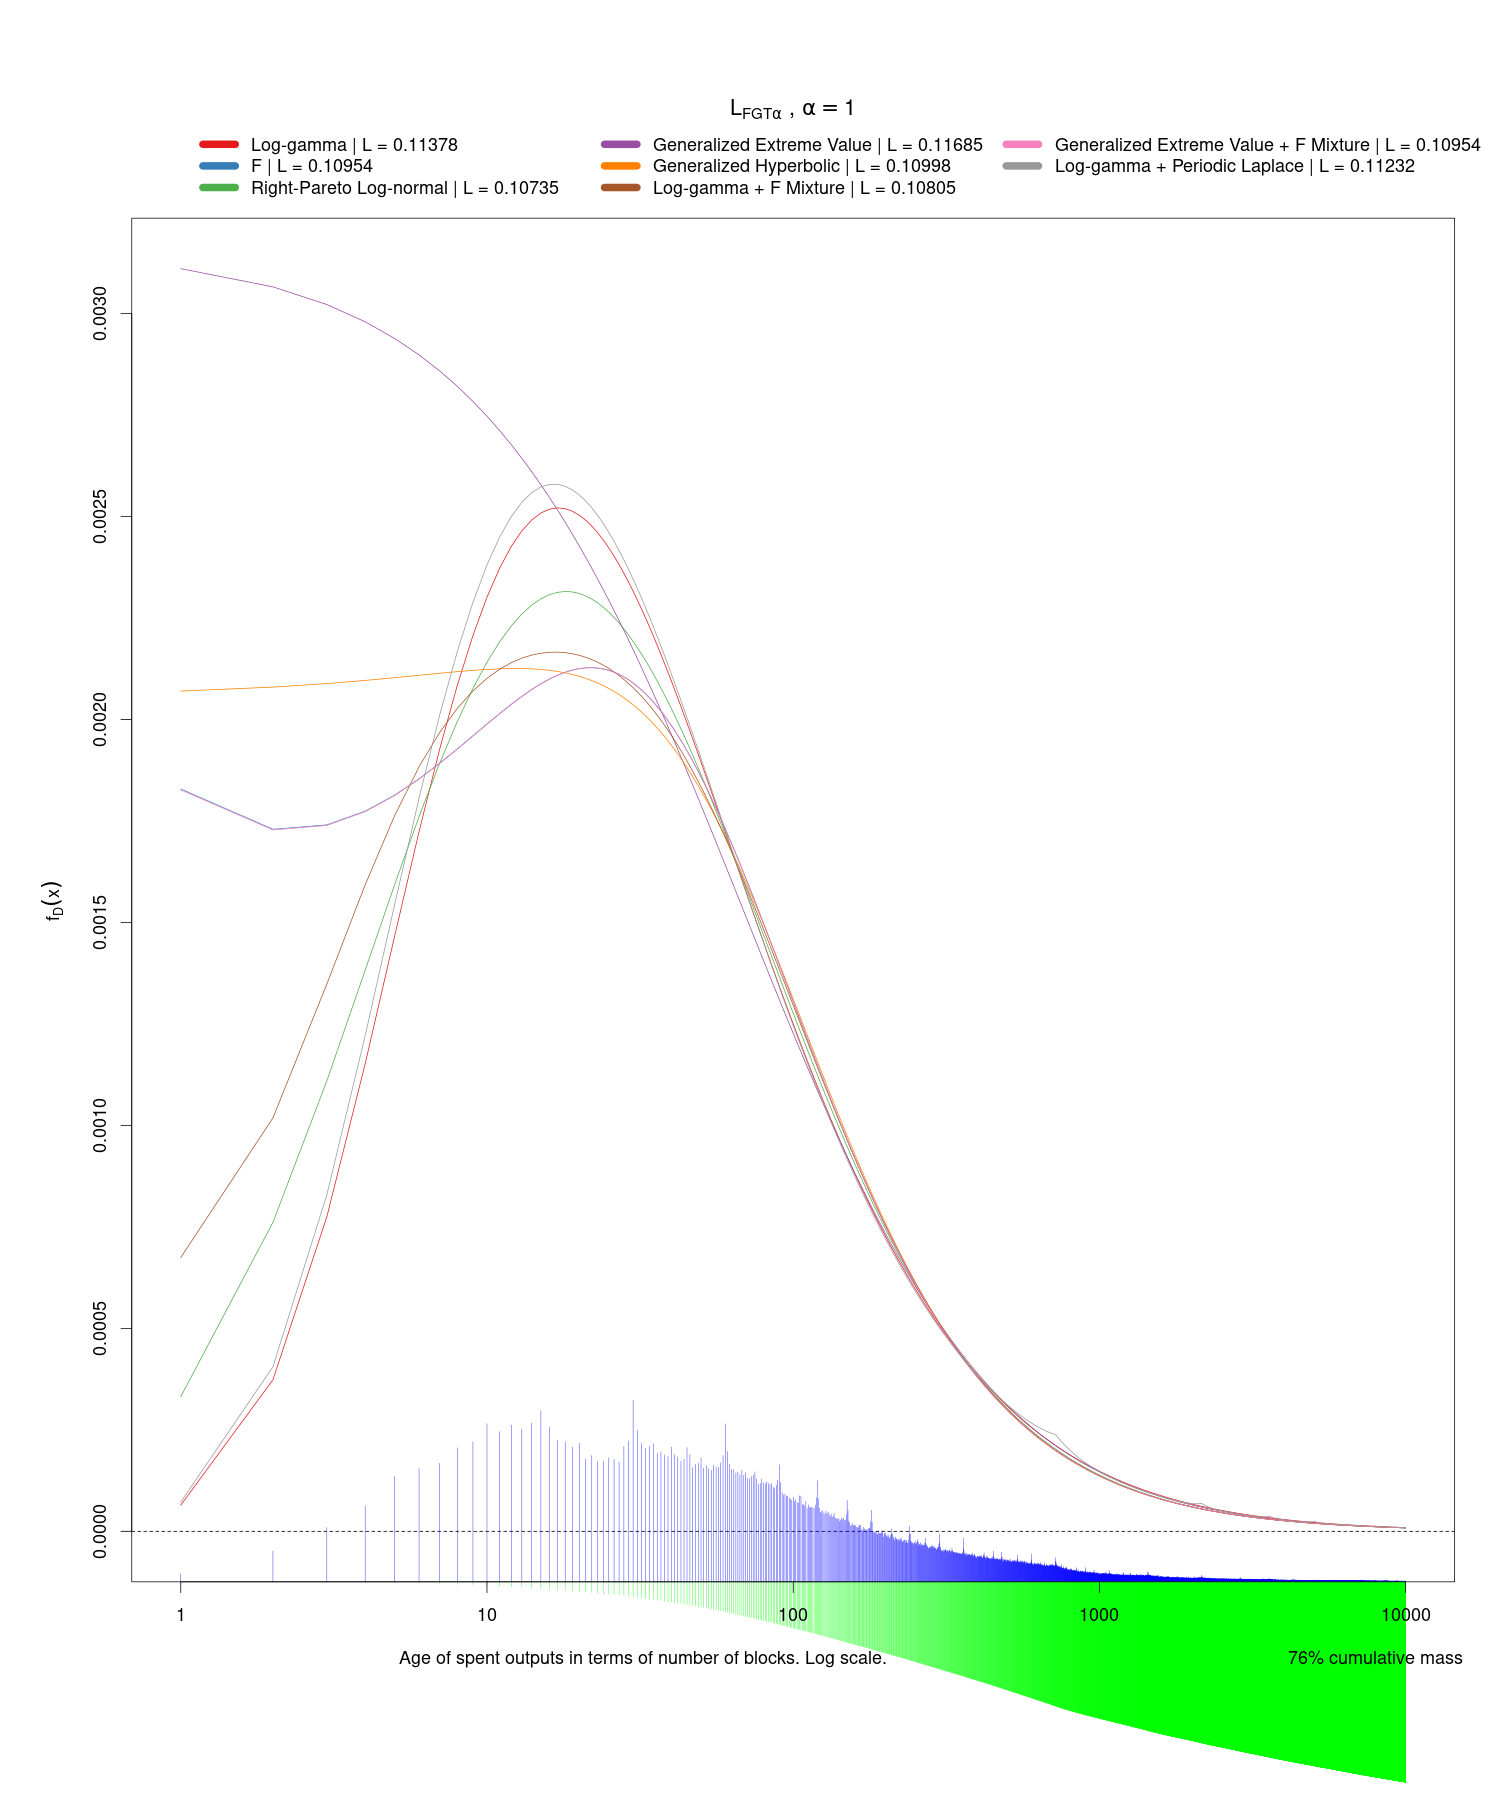
\includegraphics[scale=0.35]{images/dry-run/estimate/estimate-L_FGT-flavor-1}
\end{figure}

\begin{figure}
\caption{Optimized $f_{D}(x)$ for loss function $L_{FGT_{\alpha}}$, $\alpha=2$}

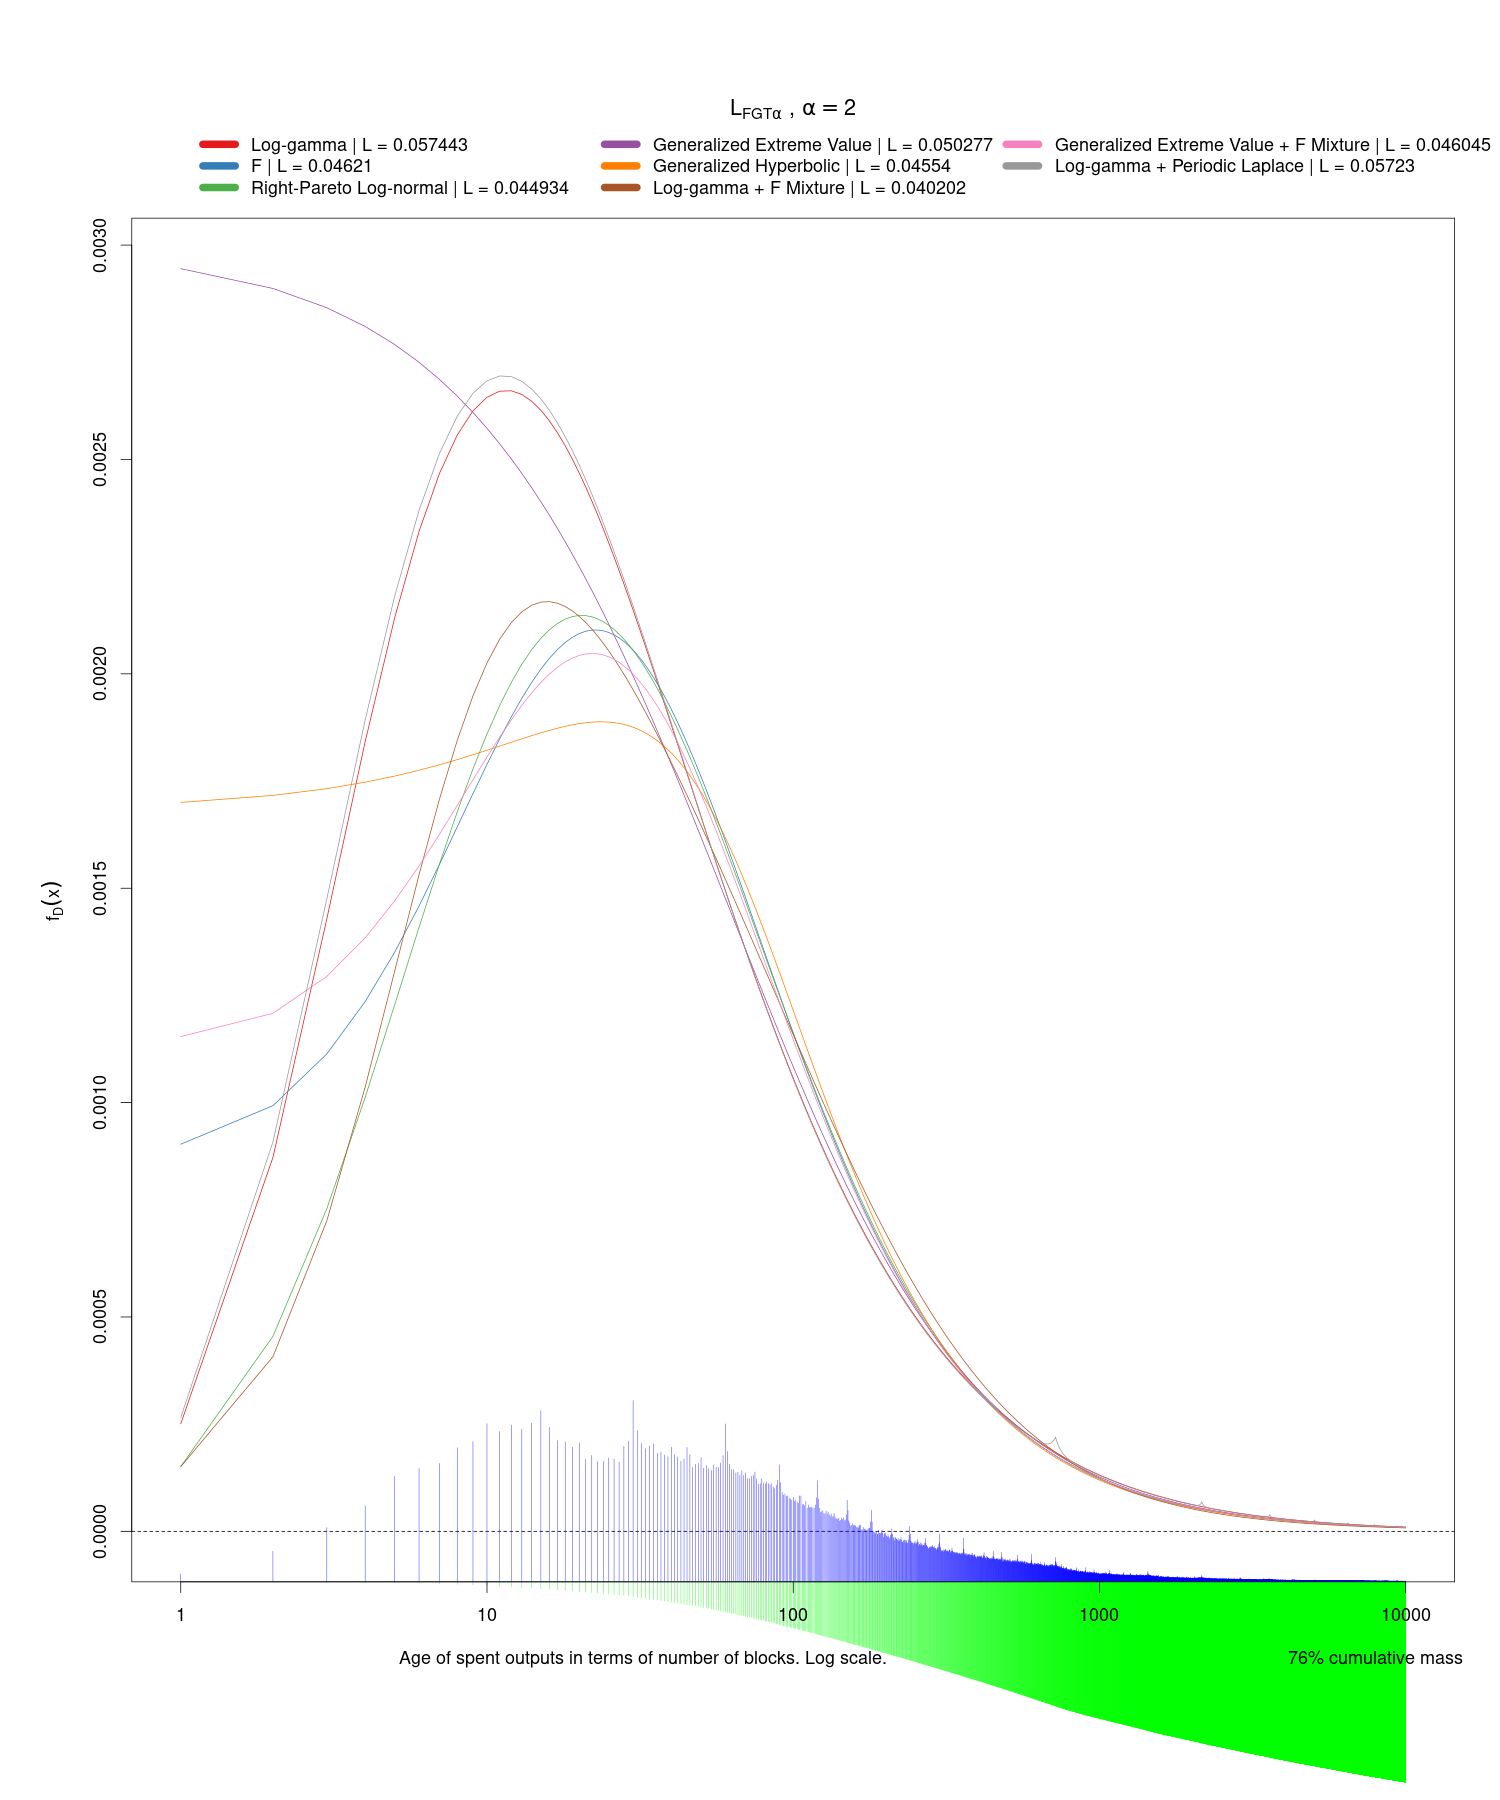
\includegraphics[scale=0.35]{images/dry-run/estimate/estimate-L_FGT-flavor-2}
\end{figure}

\begin{figure}
\caption{Optimized $f_{D}(x)$ for loss function $L_{Welfare_{\eta}}$, $\eta=0.5$}

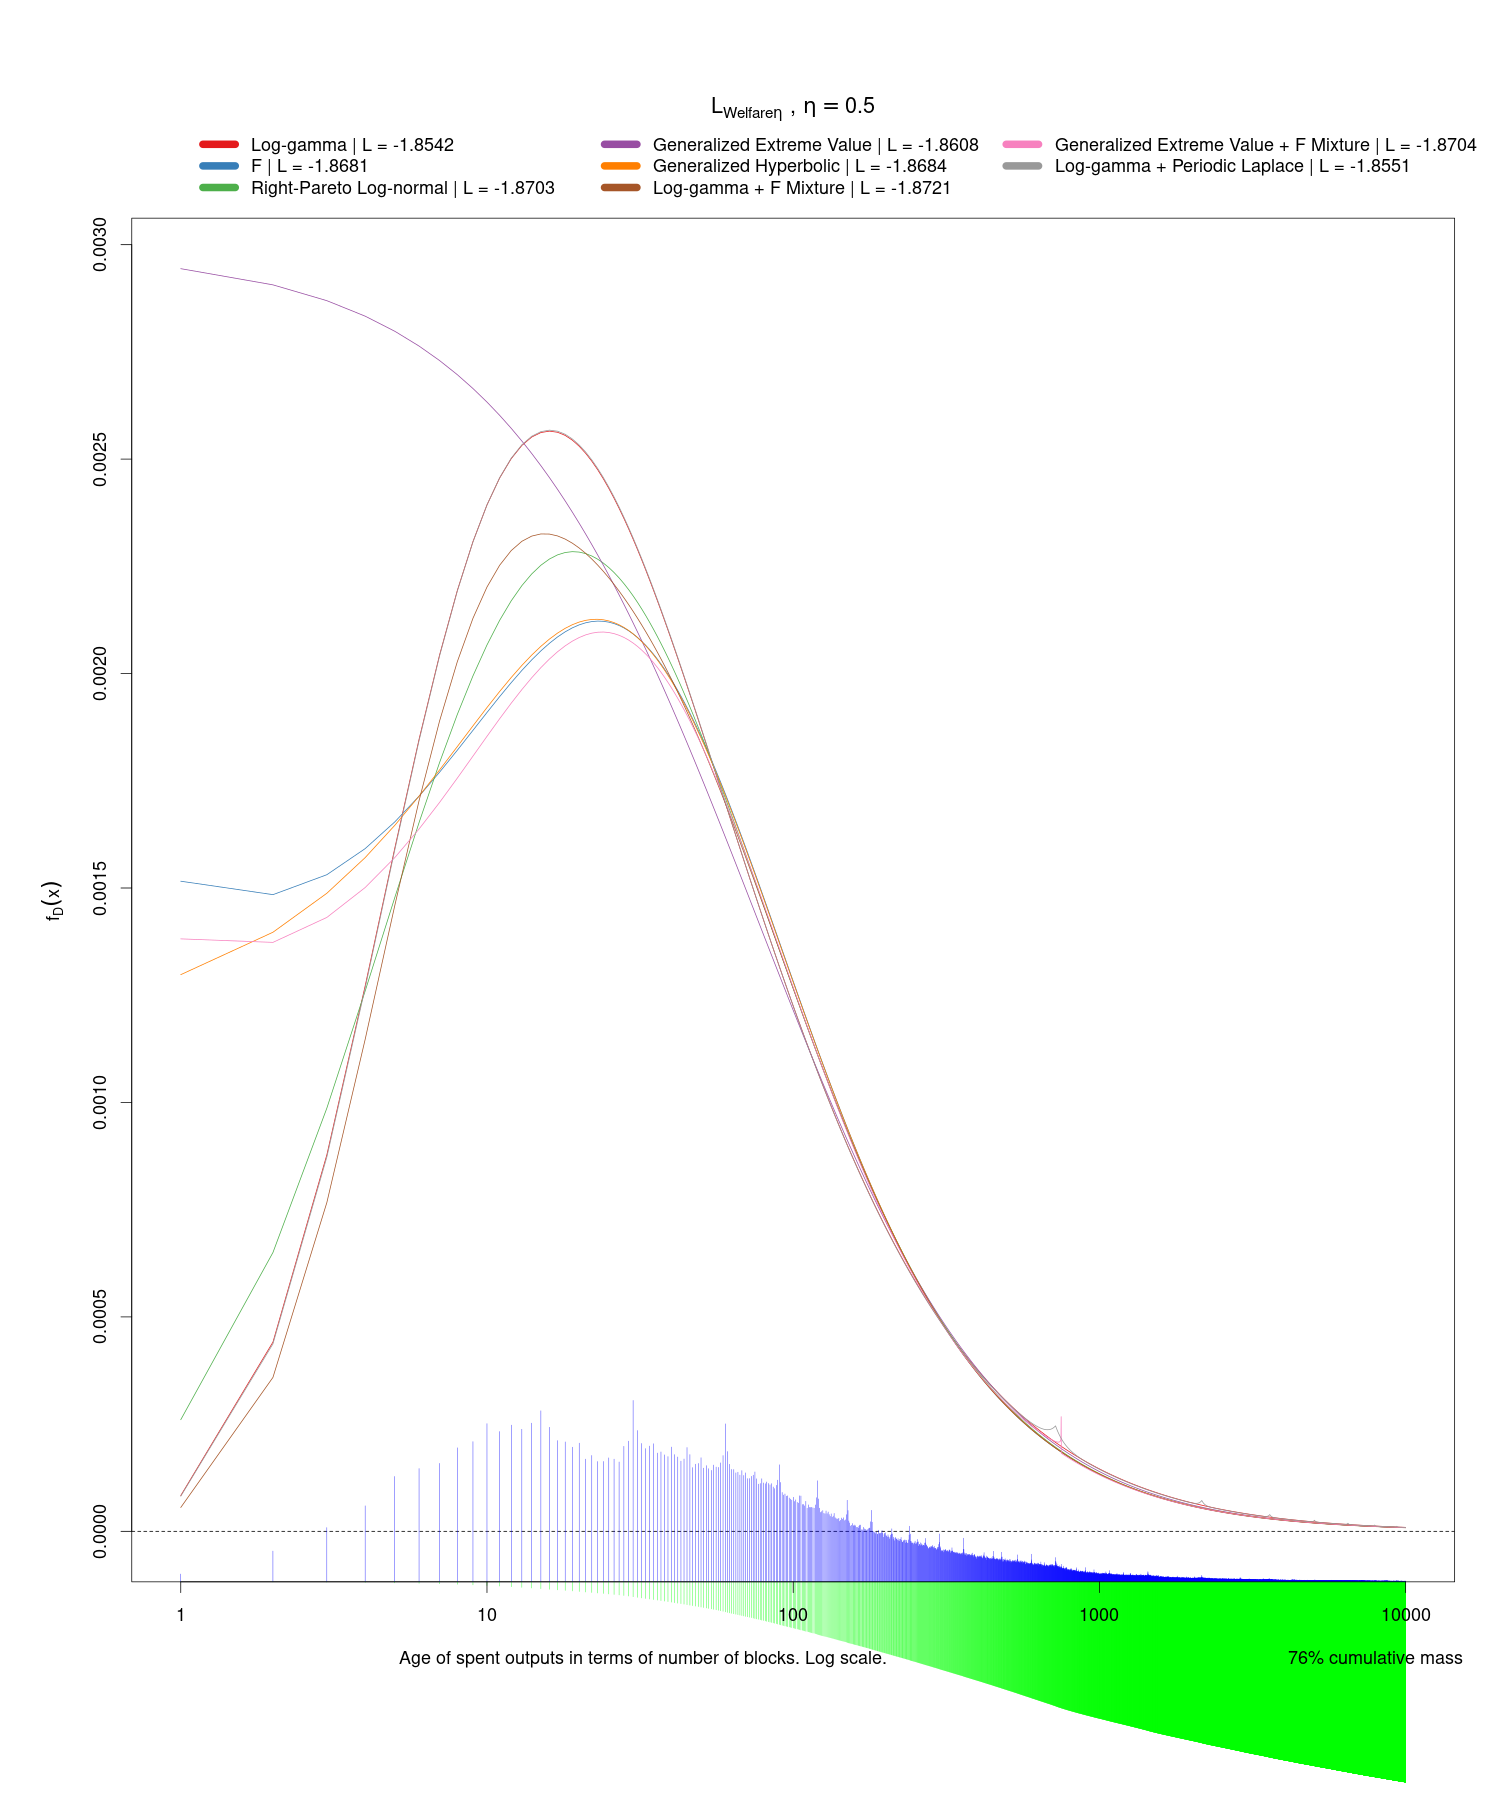
\includegraphics[scale=0.35]{images/dry-run/estimate/estimate-L_Welfare-flavor-0.5}
\end{figure}

\begin{figure}
\caption{Optimized $f_{D}(x)$ for loss function $L_{Welfare_{\eta}}$, $\eta=1$}

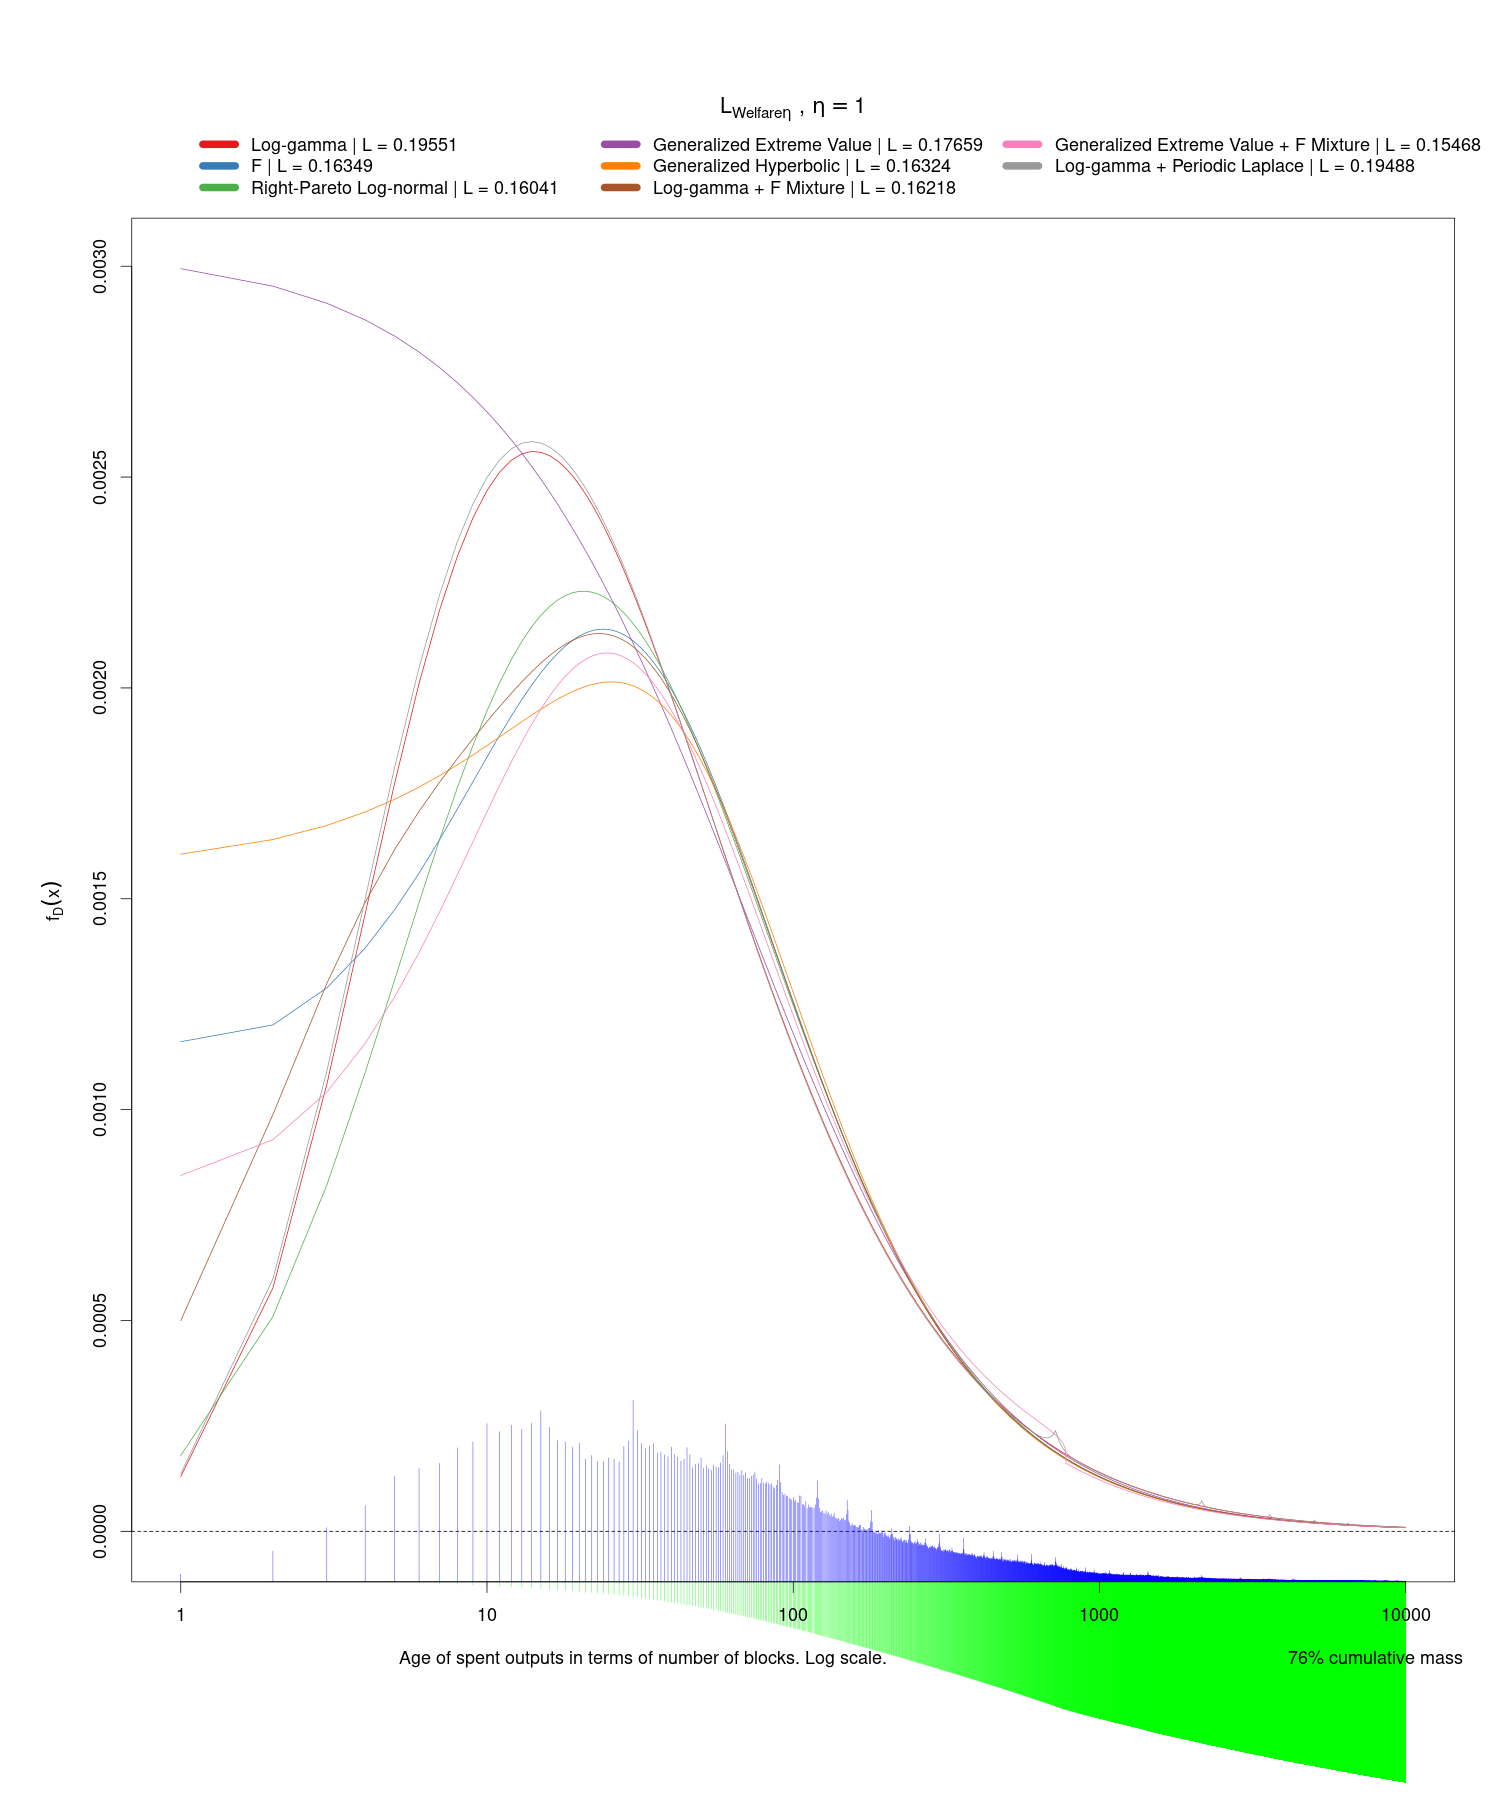
\includegraphics[scale=0.35]{images/dry-run/estimate/estimate-L_Welfare-flavor-1}
\end{figure}

\begin{figure}
\caption{Optimized $f_{D}(x)$ for loss function $L_{MLE}$}

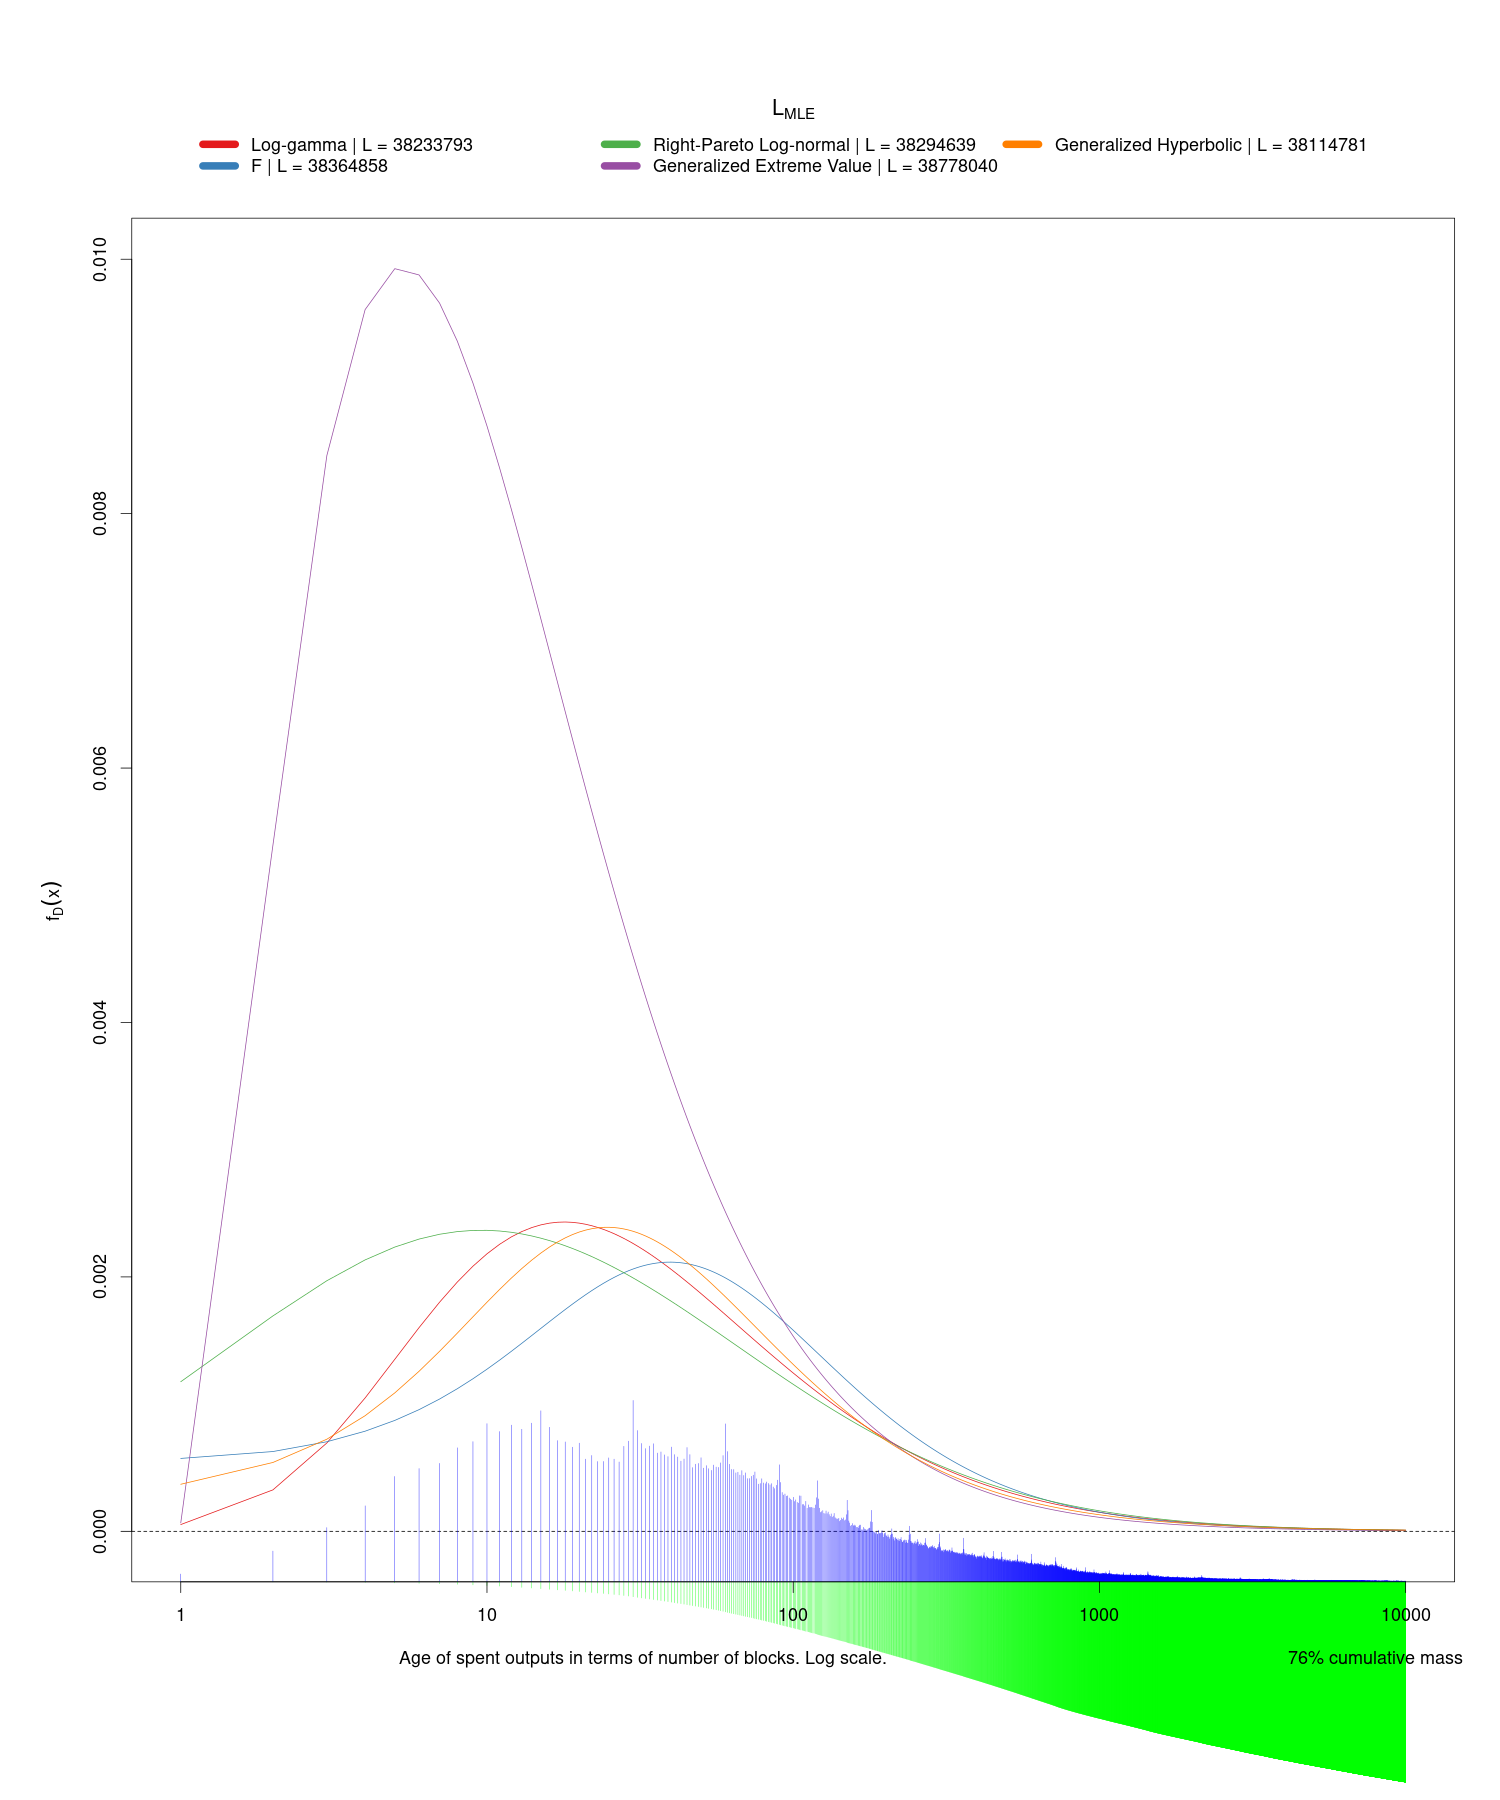
\includegraphics[scale=0.35]{images/dry-run/estimate/estimate-L_MLE-flavor-0}
\end{figure}

\begin{figure}
\caption{Optimized $f_{D}(x)/f_{S}(x)$ for loss function $L_{FGT_{\alpha}}$,
$\alpha=1$}

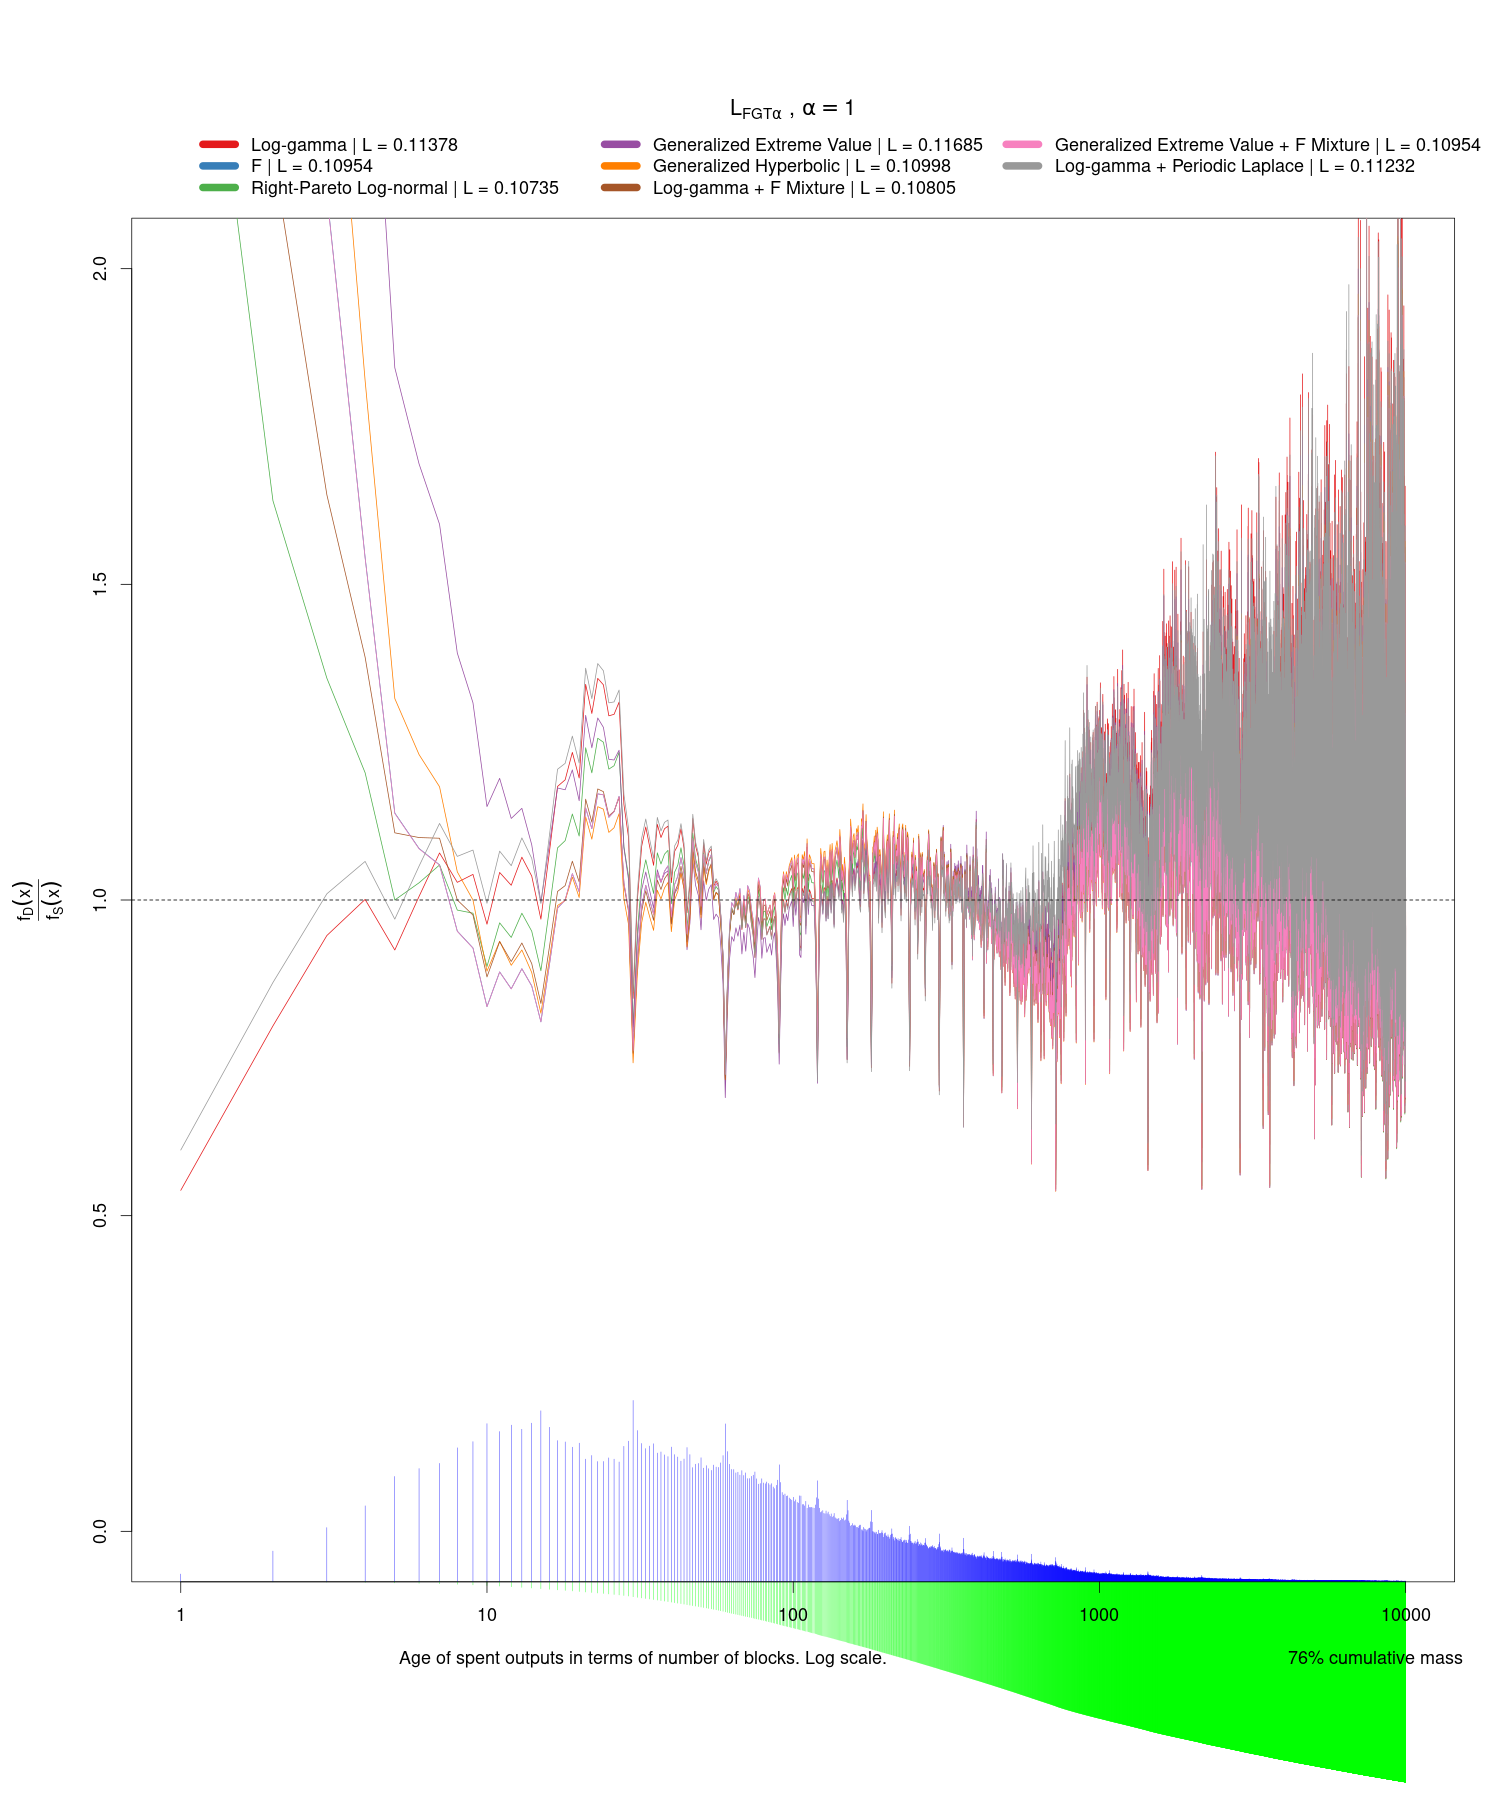
\includegraphics[scale=0.35]{images/dry-run/estimate-div-target/estimate-div-target-L_FGT-flavor-1}
\end{figure}

\begin{figure}
\caption{Optimized $f_{D}(x)/f_{S}(x)$ for loss function $L_{FGT_{\alpha}}$,
$\alpha=2$}

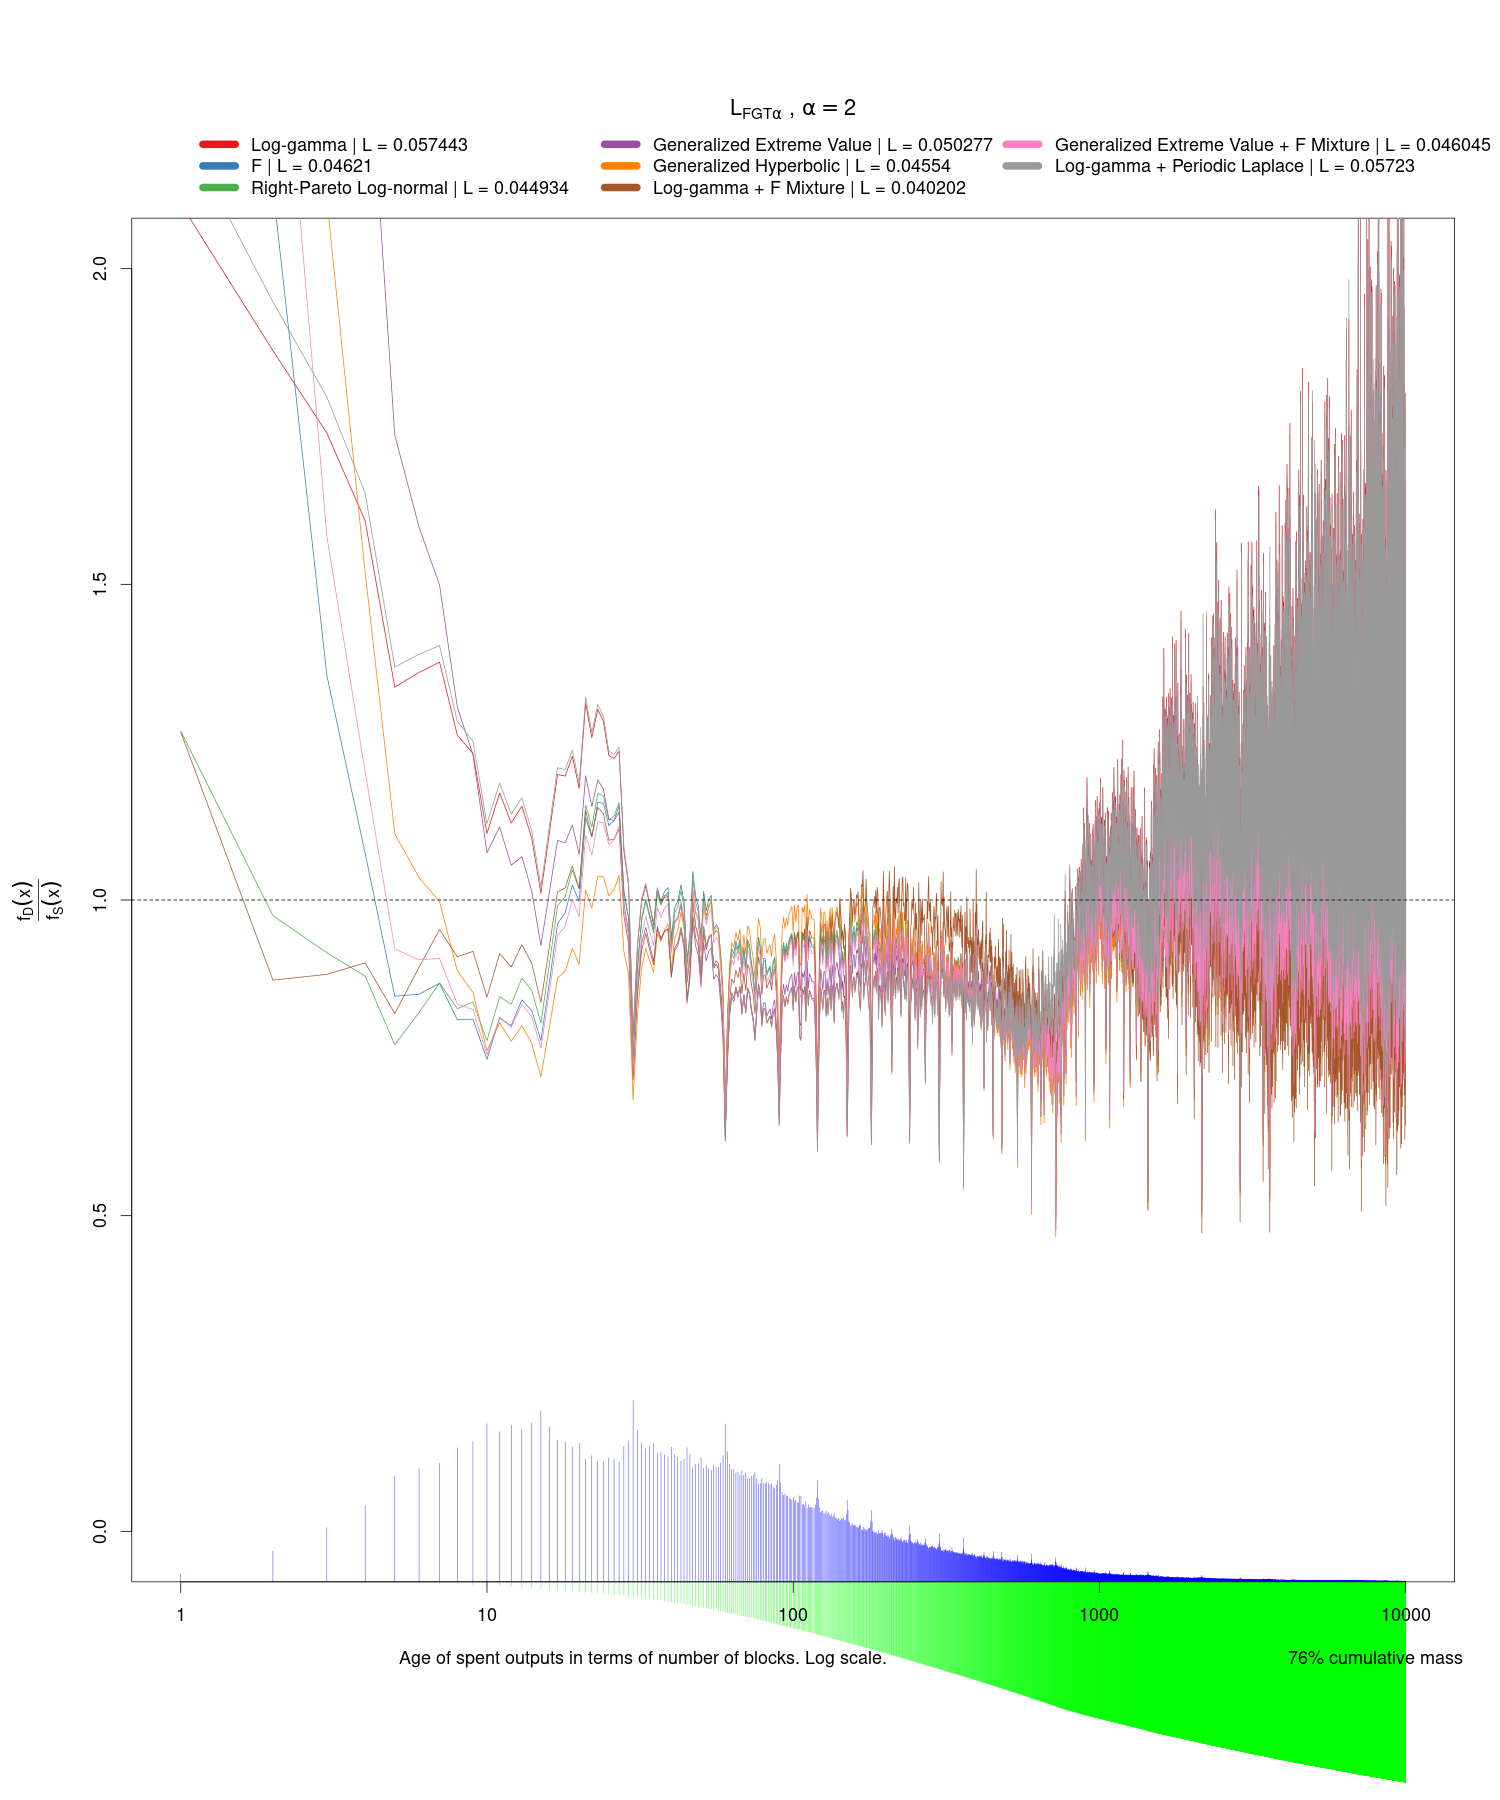
\includegraphics[scale=0.35]{images/dry-run/estimate-div-target/estimate-div-target-L_FGT-flavor-2}
\end{figure}

\begin{figure}
\caption{Optimized $f_{D}(x)/f_{S}(x)$ for loss function $L_{Welfare_{\eta}}$,
$\eta=0.5$}

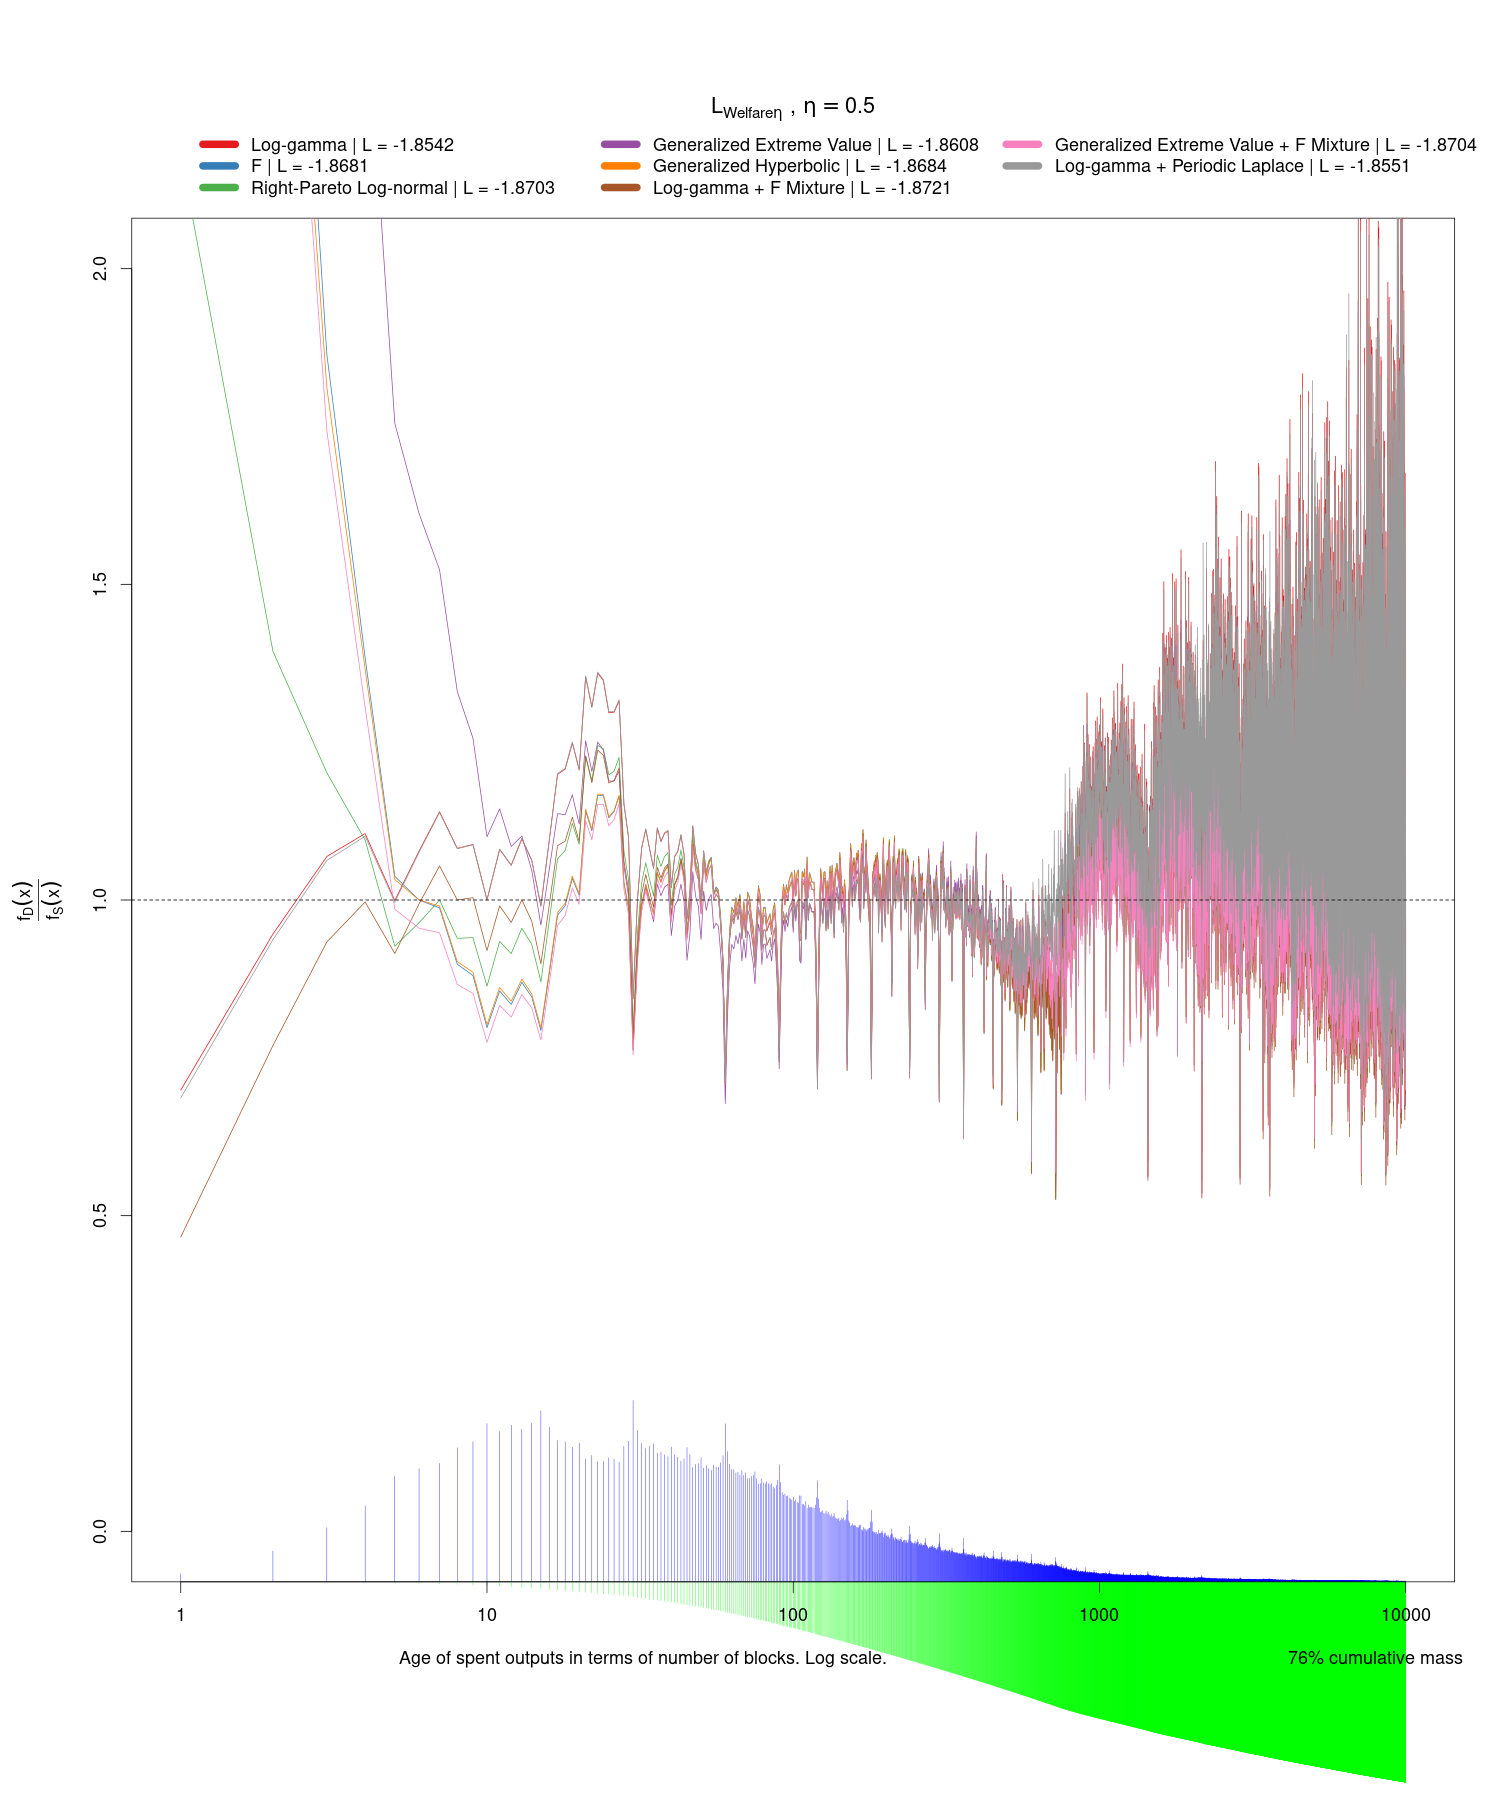
\includegraphics[scale=0.35]{images/dry-run/estimate-div-target/estimate-div-target-L_Welfare-flavor-0.5}
\end{figure}

\begin{figure}
\caption{Optimized $f_{D}(x)/f_{S}(x)$ for loss function $L_{Welfare_{\eta}}$,
$\eta=1$}

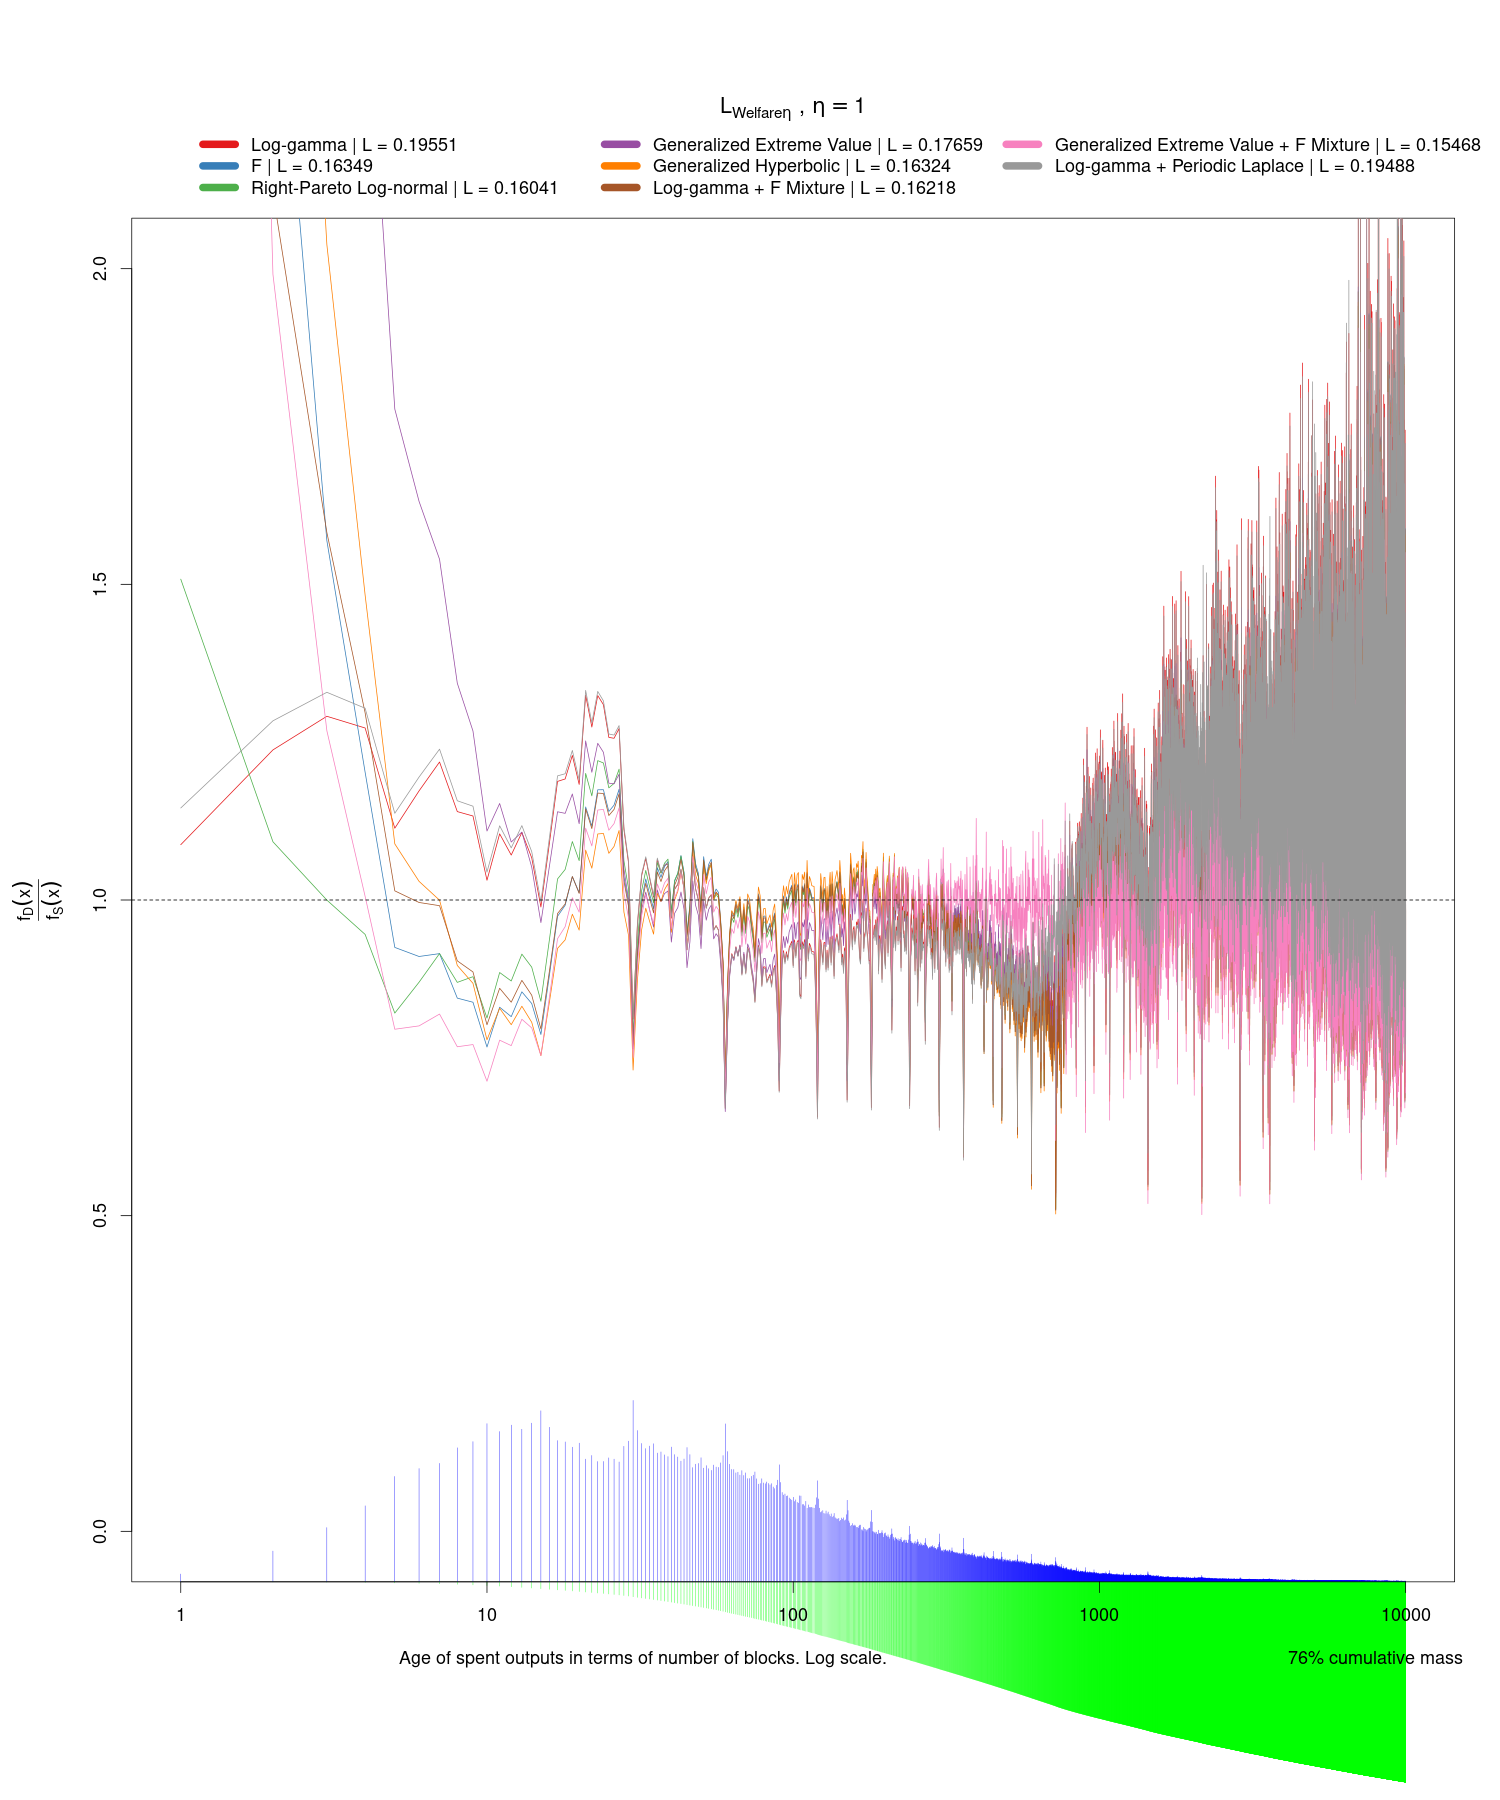
\includegraphics[scale=0.35]{images/dry-run/estimate-div-target/estimate-div-target-L_Welfare-flavor-1}
\end{figure}

\begin{figure}
\caption{Optimized $f_{D}(x)/f_{S}(x)$ for loss function $L_{MLE}$}

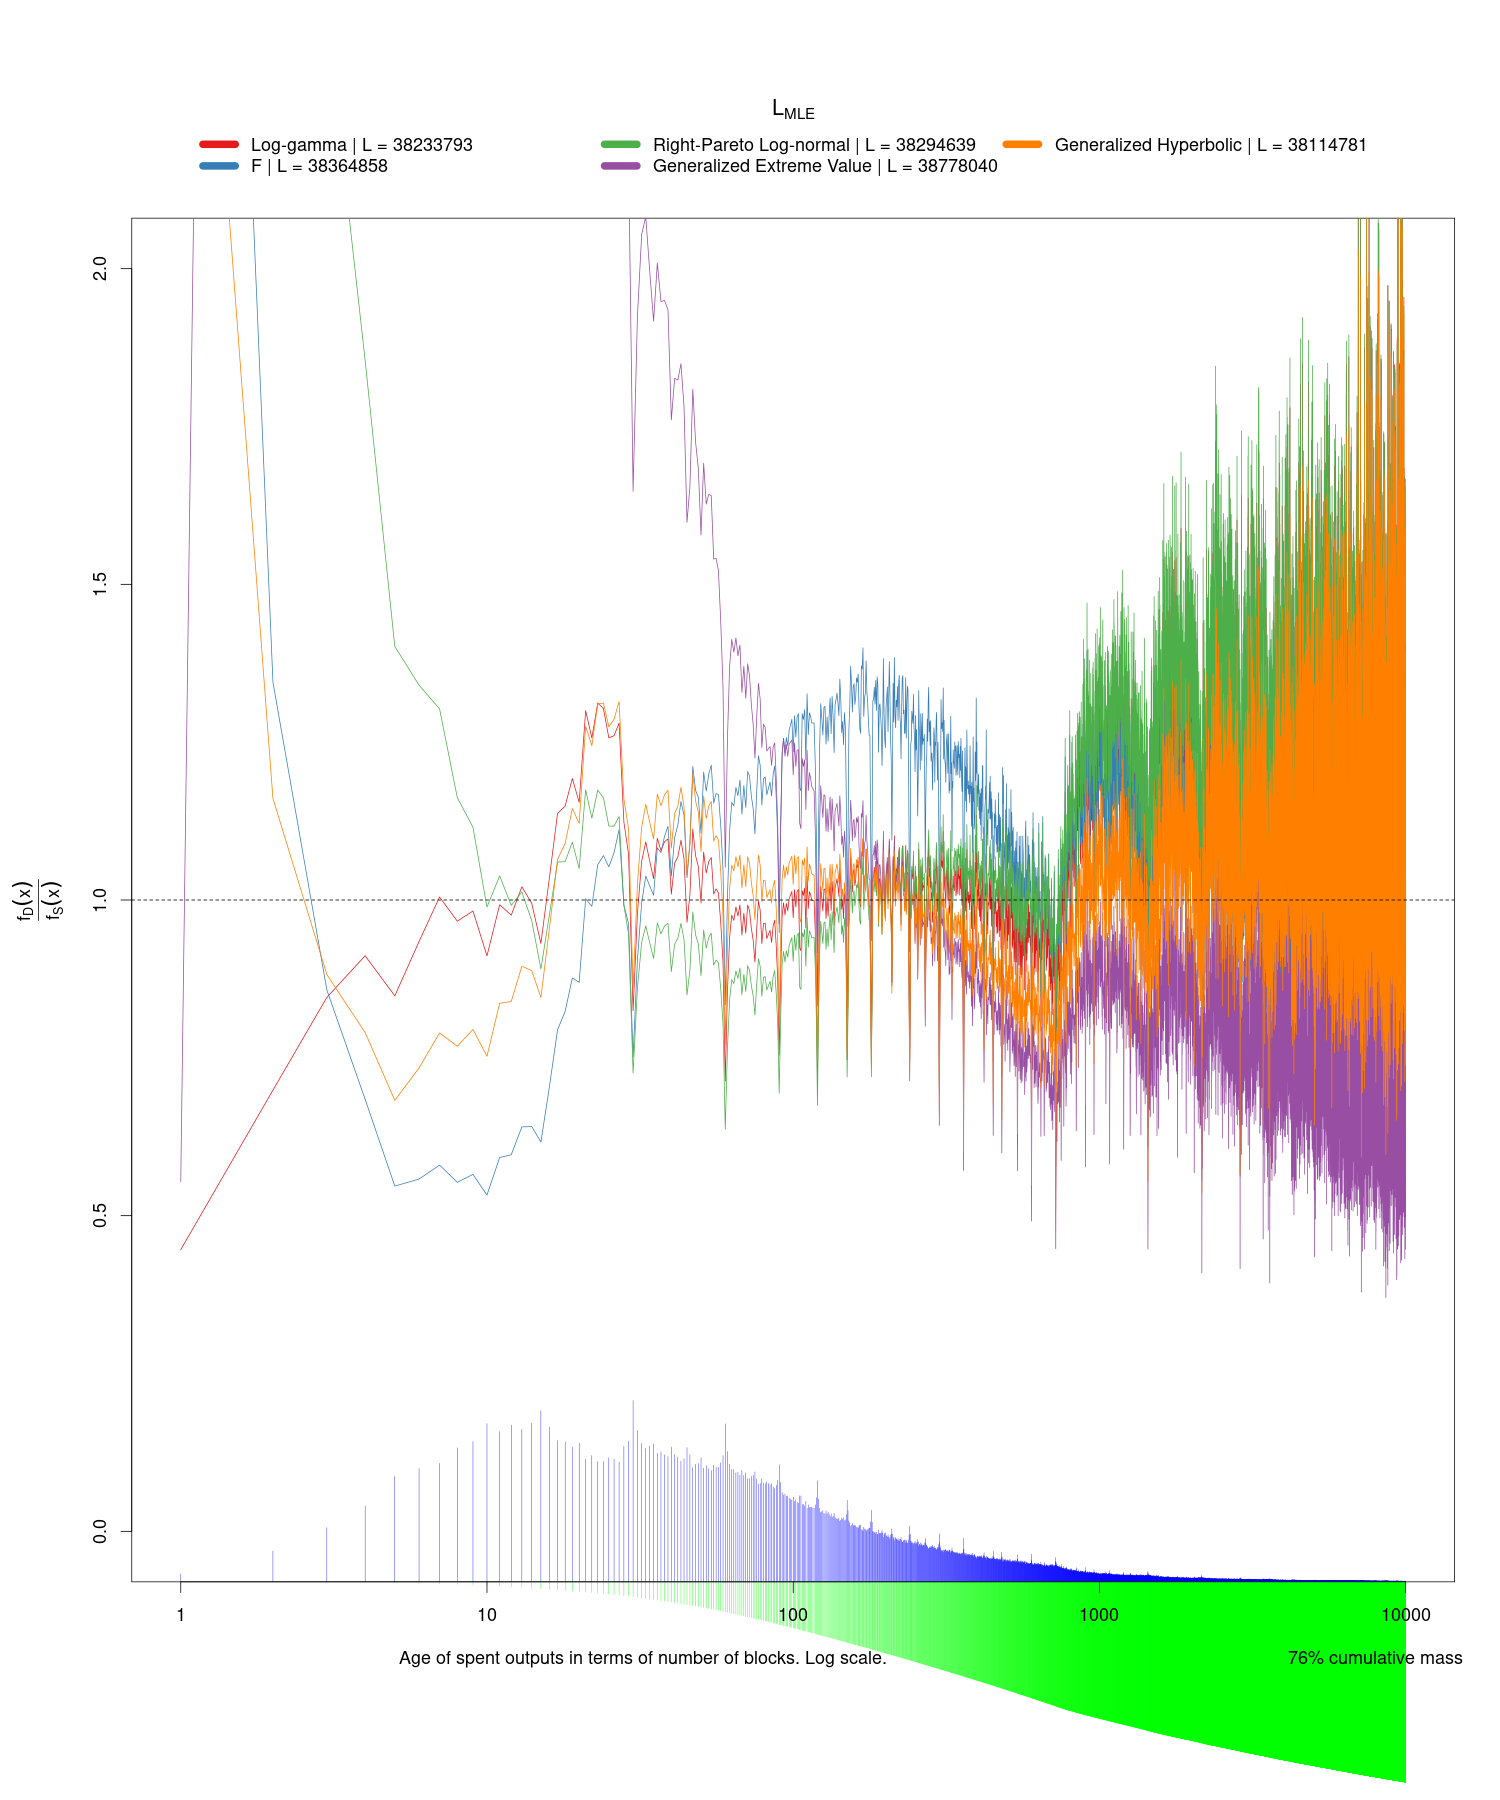
\includegraphics[scale=0.35]{images/dry-run/estimate-div-target/estimate-div-target-L_MLE-flavor-0}
\end{figure}


\section{Options for Loss Functions $\boldsymbol{\mathcal{L}}$ and Parametric
Distributions $\boldsymbol{\mathcal{F}}$\label{sec:Options-for-Loss-Functions}}

In \textbf{Section \ref{sec:Criteria-for-Best-Fit} Criteria for Best
Fit} I developed several loss functions that could be used to decide
which parametric distribution (and particular parameter values) should
be used to form the OSPEAD decoy selection algorithm. At this point
in time, it is not necessary to decide which loss function to use.
We can perform the minimizations, examine the results, and make a
decision when we have all the information.
\begin{enumerate}
\item Privacy impoverishment. This loss function overall appears to be one
of the better choices. It is intuitive and provides options in its
$\alpha$ parameter. To minimize risk of very low coverage of certain
intervals on the probability distribution, setting $\alpha\geq2$
would probably be best.
\item Economic welfare. This criteria is less intuitive than privacy impoverishment,
but it offers another way to adjust the risk sensitivity with its
$\eta$ parameter. Setting $\eta\geq1$ will force more risk avoidance.
\item Inequality minimization. This criteria would be most important if
we seek to minimize inequality among users. One of its main drawbacks
is that is can be computationally expensive.
\item Worst-case-scenario minimization. This criteria has some appeal because
worst case scenarios seem to be a focus in the field of cryptography.
However, focusing on the worst case out of hundreds of thousands may
be questionable.
\item Maximum Likelihood Estimation. \cite{2018} used this criteria. For
reasons stated above, I do not recommend this one.
\item Maximize resistance to a specific attack. This criteria has some intuitive
appeal: defend against an attack directly. However, it is difficult
to say whether maximizing resistance to one attack may leave users
vulnerable to a different attack.
\end{enumerate}
There is no particular statistical theoretical reason to choose one
parametric distribution over another. Issues with software implementation
may push us to use a simpler and more common distribution. If wallet
developers do not use the \texttt{wallet2} implementation, they may
have difficulty implementing a distribution defined by a mixture of
unusual distributions.

\newpage{}

\section{Dynamic Risk and Forecasting\label{sec:Dynamic-Risk-and-Forecasting}}

The Monero Research Lab research bulletin that I quoted in the introduction
continues with the following observation \cite{Mackenzie2015}:
\begin{quote}
This would suggest that we, the developers of Monero, must estimate
the probability distribution governing the age of transaction outputs.

This, too, is problematic. When an exchange rate is experiencing a
strong long-term decline (inflation), rational users are more likely
to spend their transaction outputs, for tomorrow their outputs will
be worth less in terms of goods and services than today and hoarding
is not economically rational. When an exchange rate is experiencing
a strong long-term increase (deflation), rational users are more likely
to hoard their transaction outputs for the opposite reason. Hence,
the distribution of transaction output ages will at least vary over
time, and, presuming any proportion of users are rational will certainly
depend sensitively on the economic performance of the currency. It
is unwise to design security recommendations around the economic performance
of our protocol.
\end{quote}
I would argue that, as long as Monero is committed to using a mimicking
decoy selection algorithm, ``design{[}ing{]} security recommendations
around the economic performance of our protocol'' is unavoidable,
if unfortunate. The best that we can do is to minimize the risk of
guessing the future distribution incorrectly. This requires an assessment
of dynamic risk with forecasting. According to empirical evidence
from transparent chains, the spent output age distribution is affected
more by volatility than long-term inflation and deflation. \cite{MakarovSchoar2021}
concluded that ``the vast majority of Bitcoin transactions between
real entities are for trading and speculative purposes. Starting from
2015, 75\% of real bitcoin volume has been linked to exchanges or
exchange-like entities such as on-line wallets, OTC desks, and large
institutional traders.'' I discussed my own findings for DOGE in
the June 1, 2022 Monero Research Lab meeting.\footnote{\href{https://libera.monerologs.net/monero-research-lab/20220601\#c103366}{https://libera.monerologs.net/monero-research-lab/20220601\#c103366}}
The transaction patterns of Monero may be somewhat different due to
its absence from many centralized exchanges, but probably not completely
different. Assume for a moment that changes in the real spend age
distribution are entirely caused by exchange rate volatility. In that
case, forecasting the real spend age distribution would be roughly
equivalent to forecasting exchange rate volatility and therefore would
be highly challenging. The Efficient Market Hypothesis would imply
that a naive forecast may be the best forecast.

We return to Equation (\ref{eq:risk-function-general}) from \textbf{Section
\ref{sec:Criteria-for-Best-Fit} Criteria for Best Fit}: the risk
function $R(\theta,\delta)=\mathrm{E}_{\theta}L(\theta,\delta(\mathbf{X}))$.
This is the expected value of our choice of the loss function when
a particular set of parameters, e.g. the shape, scale, and location
of a parametric distribution, are set to particular values. The theoretical
bounds on $R(\theta,\delta)$ can be very wide in our setting and
do not grant us much guidance. Therefore, it is best to compute some
sort of empirical risk function based on data. All we have is past
data, yet our goal is to compute future risk. We must forecast future
data and then determine performance of our various options of decoy
selection algorithms through forecast validation.

How to do forecasting and forecast validation? A naive, simple method
to forecast future values is to assume that the values will be the
same as in the current period. More sophisticated methods attempt
to anticipate changes in the forecasted values by analyzing cycles
and statistical dependence of the values. In our setting with multivariate
forecasting, some appropriate forecasting methods include Exponential
Smoothing, Vector Autoregression (VAR), Vector Autoregressive Moving
Average (VARMA), Generalized Autoregressive Conditional Heteroskedasticity
(GARCH), and Kalman Filter.

Cross-validation is a popular general method to evaluate model accuracy.
There are special considerations when the data is time series because
time series data is not necessarily independent nor identically distributed.
The general consensus in the academic literature is that when the
characteristics of the time series are unknown then ``out-of-sample''
(OOS) cross-validation should be used. OOS cross-validation fits a
forecasting model on all the data except the last few periods and
then measures how well the model forecasts the data of the last few
periods. OOS cross-validation is also known as ``last block validation'',
``forward validation'', and ``holdout validation'' (\cite{BERGMEIR2012192},
\cite{Cerqueira2020}).

To be specific, what I mean by ``unknown'' characteristics of a
time series is that it is unknown whether the time series is stationary.
Stationarity is a technical condition in time series that requires
that its distribution does not depend on time. An independent and
identically distributed series is stationary. A series that is neither
independent nor identically distributed will not be stationary. Many
financial time series are non-stationary. A common way to manage non-stationarity
in data is to compute the first difference (or second difference if
necessary, or third...), but it is not clear how this could be done
when the object of observation is an entire distribution, as it is
in our setting.

\cite{BERGMEIR201870} mathematically prove that standard $K$-fold
cross-validation is a valid technique when the data series is stationary
(plus a few other assumptions). They warn that $K$-fold cross-validation
is not valid if the data series is non-stationary and show through
Monte Carlo simulations that OOS validation performs better on non-stationary
data. \cite{BERGMEIR2012192} arrive at a similar conclusion. \cite{Cerqueira2020}
separate dozens of real data sets into stationary and non-stationary
and finds that ``when the time series are non-stationary, the most
accurate estimates are produced by out-of-sample methods, particularly
the holdout approach repeated in multiple testing periods....When
the observations in a data set are not i.i.d. {[}independently and
identically distributed{]}, the standard cross-validation approach
is not directly applicable.'' The top performing models in the M5
forecasting competition generally used the last 28 day period for
cross-validation (\cite{MAKRIDAKIS2022}).

There is no particular reason to think that the spent output age distribution
is stationary. Certainly, research into spent output age is in its
infancy. Non-stationarity is the weaker assumption. To be ``safe''
it is better to impose fewer assumptions on statistical models if
we cannot justify them. Furthermore, with only about 52 weeks of Monero
data it would be difficult to perform a formal hypothesis test of
stationarity with high statistical power. Therefore, it is best to
use OOS cross-validation to evaluate forecast accuracy and risk. A
form of OOS cross-validation is performed in the following section.

The \texttt{tsqsim} software created by Monero developer mj-xmr is
capable of OOS cross-validation.\footnote{\href{https://github.com/mj-xmr/tsqsim}{https://github.com/mj-xmr/tsqsim}}
Some modifications will be necessary to support multivariate time
series. Technically, spent output age is univariate, but since we
are measuring the age \textit{distribution} at each time period, it
makes sense to model it in a multivariate way.

\section{Inter-Temporal Stability of Spent Output Age Distribution for BTC,
BCH, LTC, and DOGE\label{sec:Inter-Temporal-Stability}}

Much like in \textbf{Section \ref{sec:Dry-Run-with-Old-Moser-et-al-Data}
Dry Run with Old M{\:o}ser et al. (2018) Data}, it is useful to run an
analysis of similar spent output age data from other blockchains to
inform statistical modeling strategies. 

The table below lists the share of payments made with several different
cryptocurrencies with an unspent transaction output (UTXO) model.
I ignored cryptocurrencies with an account model like Ethereum because
the spending mechanism is fundamentally different. The main question
that we want to answer is whether the chosen cryptocurrencies are
used in a roughly similar manner to Monero: as peer-to-peer electronic
cash. This table may suggest that BTC, BCH, LTC, and DOGE have somewhat
similar usage as Monero. One major difference between these cryptocurrencies
and Monero is that there is a 10 block lock enforced at the protocol
level for Monero. BTC, BCH, LTC, and DOGE allow users to spend received
funds immediately.
\begin{center}
\begin{tabular}{|c|c|r|r|r|r|r|r|}
\hline 
\multicolumn{8}{|c|}{\textbf{UTXO-based cryptocurrency usage as payment by percent (payment
processors and merchants)}}\tabularnewline
\hline 
 & \textbf{Service} & Bitpay\footnote{\href{https://bitpay.com/stats/}{https://bitpay.com/stats/}} & CoinCards\footnote{\href{https://twitter.com/CoinCards/status/1555286172385116164}{https://twitter.com/CoinCards/status/1555286172385116164}} & Bitrefill\footnote{\href{https://youtu.be/bkjEcSmZKfc?t=549}{https://youtu.be/bkjEcSmZKfc?t=549}} & Cake Pay\footnote{\href{https://twitter.com/cakewallet/status/1565370179906838528}{https://twitter.com/cakewallet/status/1565370179906838528}} & Travala\footnote{\href{https://travala-dashboard.com/}{https://travala-dashboard.com/}} & Shodan\footnote{\href{https://blog.shodan.io/accepting-crypto-a-vendor-perspective/}{https://blog.shodan.io/accepting-crypto-a-vendor-perspective/}}\tabularnewline
\hline 
\hline 
 & \textbf{TXs/month} & 67,000 & NA & 186,000 & NA & NA & 220 total\tabularnewline
\hline 
 & \textbf{Time period} & June 2022 & July 2022 & NA & Aug 2022 & NA & NA\tabularnewline
\hline 
 & \textbf{Metric} & Transactions & USD value & Unique users & USD value & Hotel nights & Subscriptions\tabularnewline
\hline 
BTC &  & 53.3 & 41.0 & 40 & 16 & 9.2 & 47.3\tabularnewline
\hline 
BCH &  & 5.0 & NA & NA & NA & 0.5 & 4.1\tabularnewline
\hline 
LTC &  & 21.2 & 7.0 & 7 & 6 & 0.8 & 12.7\tabularnewline
\hline 
DOGE &  & 6.2 & 3.0 & NA & NA & 0.3 & 13.2\tabularnewline
\hline 
XMR &  & NA & 19.0 & NA & 78 & 1.9 & NA\tabularnewline
\hline 
DASH &  & NA & 0.5 & NA & NA & 0.5 & NA\tabularnewline
\hline 
ADA &  & NA & NA & NA & NA & 0.9 & NA\tabularnewline
\hline 
\end{tabular}
\par\end{center}

In the next several section I perform statistical analysis of these
four UTXO cryptocurrencies. The code is available at \href{https://github.com/Rucknium/OSPEAD/tree/main/General-Blockchain-Age-of-Spent-Outputs}{https://github.com/Rucknium/OSPEAD/tree/main/General-Blockchain-Age-of-Spent-Outputs}.
The code was executed on the Monero Research Computing Server, whose
hardware was improved by a CCS proposal.\footnote{\href{https://ccs.getmonero.org/proposals/gingeropolous_zenith_storage.html}{https://ccs.getmonero.org/proposals/gingeropolous\_zenith\_storage.html}}

\subsection{Summary Characterization of Distributions Over Time}

Figures \ref{figure-BTC-Summary-Characterization} to \ref{figure-DOGE-Summary-Characterization}
show several statistics about the age of spent outputs of BTC, BCH,
LTC, and DOGE since 2015. The age units are in terms of blocks. For
BTC and BCH the interval between blocks is 10 minutes. For LTC it
is 2.5 minutes and for DOGE it is 1 minute. The unit of observation
is the ISO week, a natural unit of economic time.\footnote{\href{https://en.wikipedia.org/wiki/ISO_week_date}{https://en.wikipedia.org/wiki/ISO\_week\_date}}

The first line graphs show the mean, median, standard deviation, skewness,
and kurtosis. The skewness and kurtosis statistics may be unfamiliar.
They are the third and fourth standardized moments of a distribution,
respectively. The moments of a distribution is defined by a power
of the expectation $\mathrm{E}[X]$, i.e. theoretical mean, of the
distribution. The $k$th moment is $\mathrm{E}[X^{k}]$. Moments extend
the concept of moving from expectation to variance (which is the square
of the standard deviation). The mean (expectation) of a random variable
is simply the first moment:

\[
\mu=\mathrm{E}[X^{1}]
\]

The variance is the second central moment:

\[
\sigma^{2}=\mathrm{E}\left[\left(X-\mathrm{E}[X]\right)^{2}\right]
\]

The skewness is the third standardized moment (standardized by the
standard deviation $\sigma$):

\[
\tilde{\mu}_{3}=\mathrm{E}\left[\left(\dfrac{X-\mathrm{E}[X]}{\sigma}\right)^{3}\right]
\]

The kurtosis is the fourth standardized moment:

\[
\tilde{\mu}_{4}=\mathrm{E}\left[\left(\dfrac{X-\mathrm{E}[X]}{\sigma}\right)^{4}\right]
\]

The mean is a measure of the central tendency of a distribution. The
standard deviation is a measure of its dispersion (spread). The skewness
and kurtosis of a distribution involve its characteristics in its
tail or tails. A positive skew means that the distribution's tail
is on the right side of the distribution. All the age distributions
analyzed here tend to have a positive skew. High kurtosis means that
large outliers are more likely. Kurtosis of greater than 3 suggests
that a distribution has a fatter tail than the normal distribution.
The skewness and kurtosis become relevant when very old outputs \textquotedblleft wake
up\textquotedblright{} during periods of exchange rate volatility
to participate in speculative activity, i.e. buying and selling on
exchanges. 

\begin{figure}

\caption{Skewness }

\begin{centering}
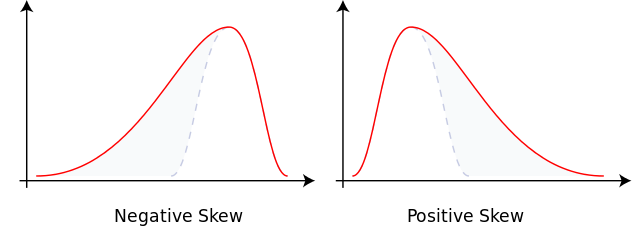
\includegraphics[scale=0.75]{images/640px-Negative_and_positive_skew_diagrams_(English).svg}
\par\end{centering}
Source: https://en.wikipedia.org/wiki/File:Negative\_and\_positive\_skew\_diagrams\_(English).svg

\end{figure}

The fitting function is essentially a minimum divergence estimator.
This means that the parameters of the parametric probability density
function (PDF) are chosen to minimize the distance between the parametric
PDF and the PDF formed by the data (the empirical PDF), for some specified
metric of \textquotedblleft distance\textquotedblright . 

There are several measures of distance that could be used. For the
purpose of this exploration of output age distribution forecasting,
the distance metric to be minimized will be the total linear sum of
the mass of the estimated parametric PDF that falls below the empirical
PDF. With the \textquotedblleft loss function\textquotedblright{}
specified this way, the optimization algorithm attempts to minimize
the probability that the real spends are much more likely to come
from a block of a particular age compared to a potential decoy. Ideally,
the decoy distribution would be identical to the real spend age distribution,
but parametric PDFs are not flexible enough to perfectly match an
empirical PDF.

Define $f_{S}(x)$ as the empirical spent output age distribution
at block age $x$ and $f_{D}(x;\boldsymbol{\beta})$ as a potential
\textquotedblleft decoy\textquotedblright{} distribution with some
parameter vector $\boldsymbol{\beta}$ (with the transparent blockchains
presented here, there is no actual decoy mechanism of course). Then
for each week of spent output age data the parameter vector $\boldsymbol{\beta}$
can be chosen to minimize this quantity:

\[
L(\boldsymbol{\beta})=\sum_{i\in\{x_{i}:f_{D}(x_{i};\boldsymbol{\beta})<f_{S}(x_{i})\}}^{N}f_{S}(x_{i})-f_{D}(x_{i};\boldsymbol{\beta})
\]

That is, minimize the sum of the difference between the real spend
age distribution for blocks $x_{i}$ where the decoy distribution
is less than the real spend age distribution. The minimization is
performed by computer numerical minimization methods similar to gradient
descent.

The two candidate \textquotedblleft decoy\textquotedblright{} parametric
PDFs under consideration in this exercise are the Log-gamma (\textit{lgamma})
distribution and the Right-Pareto Log-normal (\textit{rpln}) distribution.
The lgamma distribution, with two parameters, was used in \cite{2018}
to suggest a decoy distribution that was later incorporated into Monero's
reference wallet software. The rpln distribution is a more flexible
distribution, with three parameters. The PDFs of these two distributions
are:

\[
f_{lgamma}(x)=\dfrac{ratelog^{shapelog}}{\Gamma(shapelog)}\times\dfrac{(\ln x)^{shapelog-1}}{x^{ratelog+1}}
\]

with $ratelog>0$ and $shapelog>0$ and where $\Gamma$ is the gamma
function and

\[
f_{rpln}(x)=shape2\times x^{-shape2-1}e^{shape2\times meanlog+\frac{shape2^{2}\times sdlog^{2}}{2}}\Phi\left(\frac{\ln x-meanlog-shape2\times sdlog^{2}}{sdlog}\right)
\]

with $shape2>0$ and $sdlog>0$ and where $\Phi$ is the cumulative
distribution function of the standard Normal distribution.

\begin{figure}[H]
\caption{BTC Summary Characterization of Spend Age Distribution Over Time}
\label{figure-BTC-Summary-Characterization}

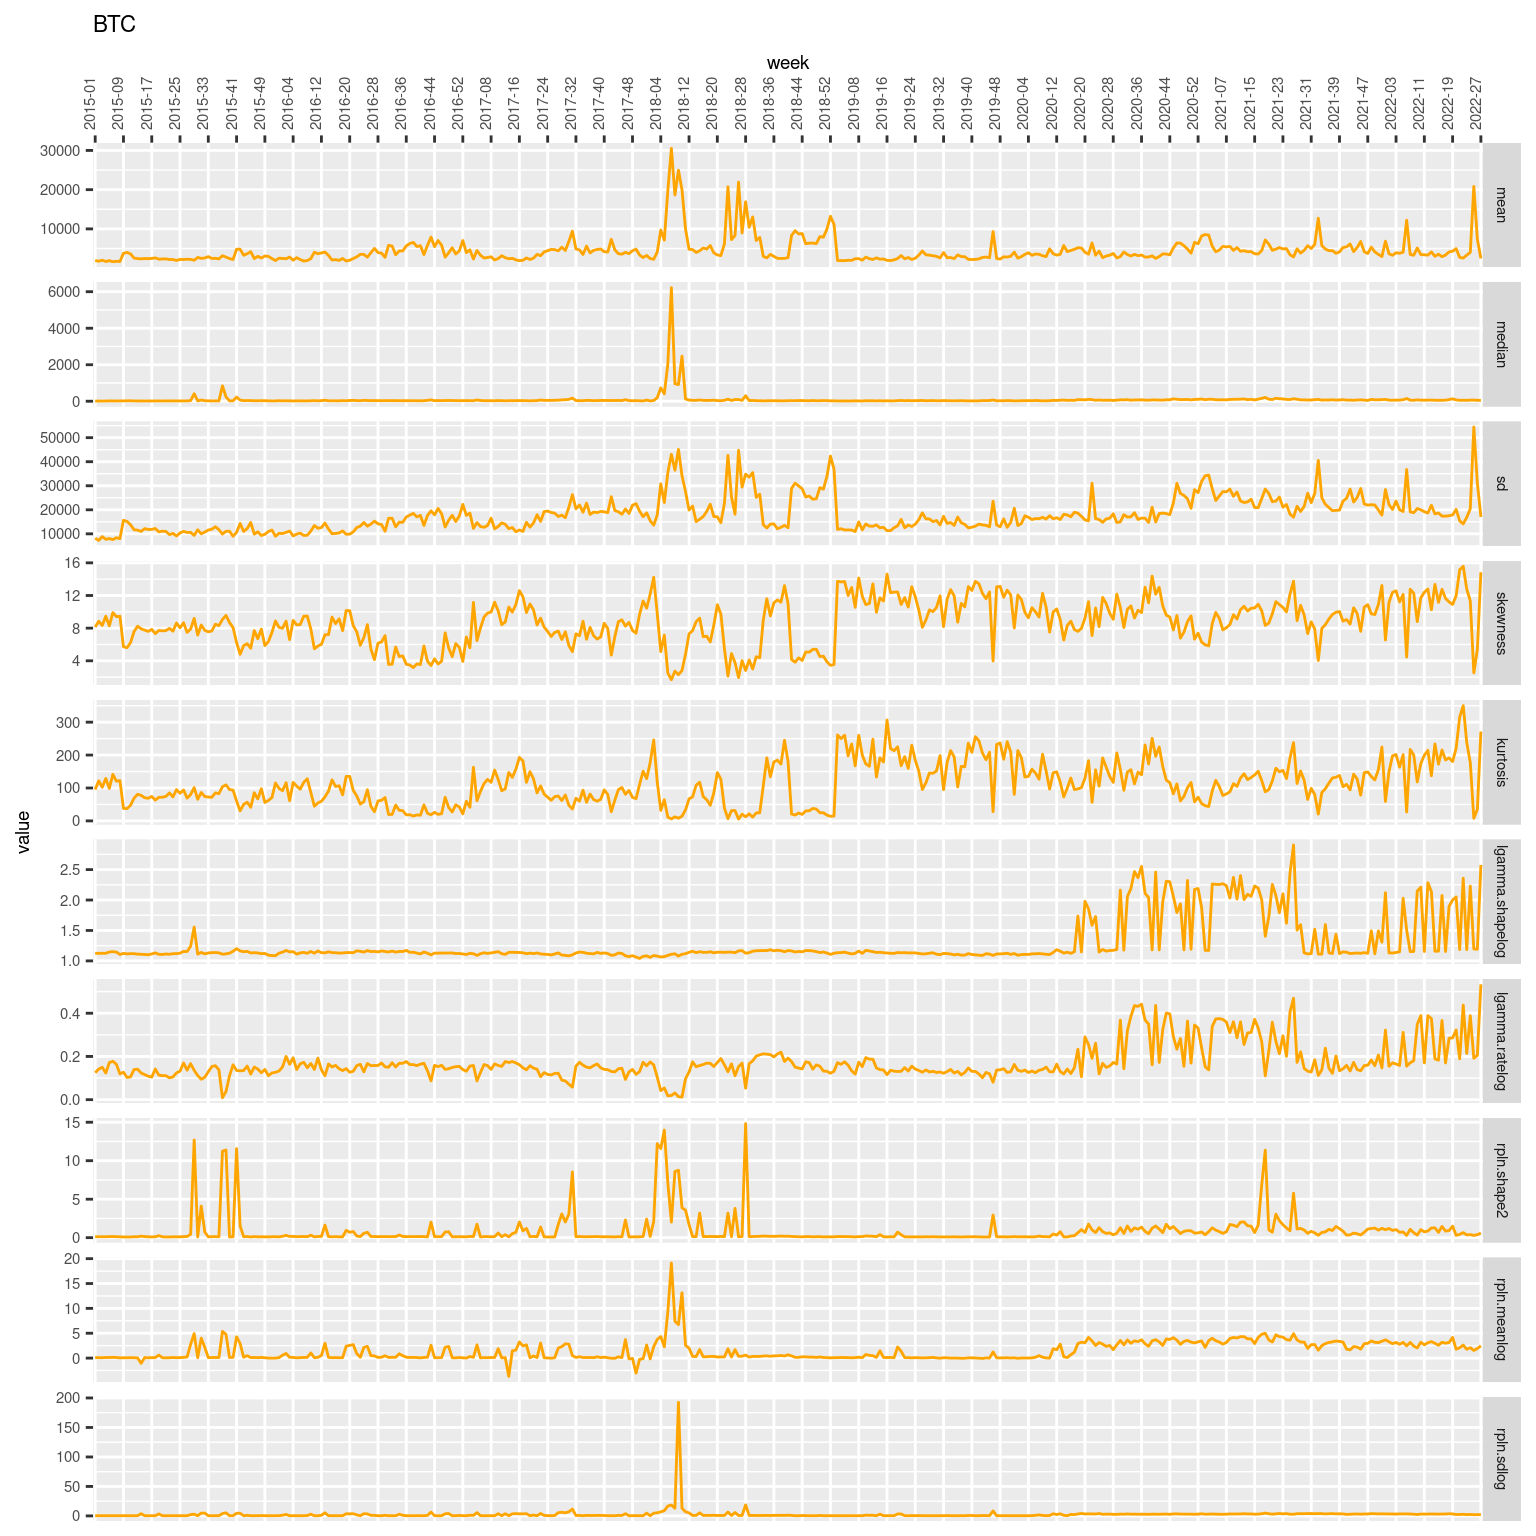
\includegraphics[scale=0.9]{images/spend-age-summary-BTC}
\end{figure}

\begin{figure}[H]
\caption{BCH Summary Characterization of Spend Age Distribution Over Time}

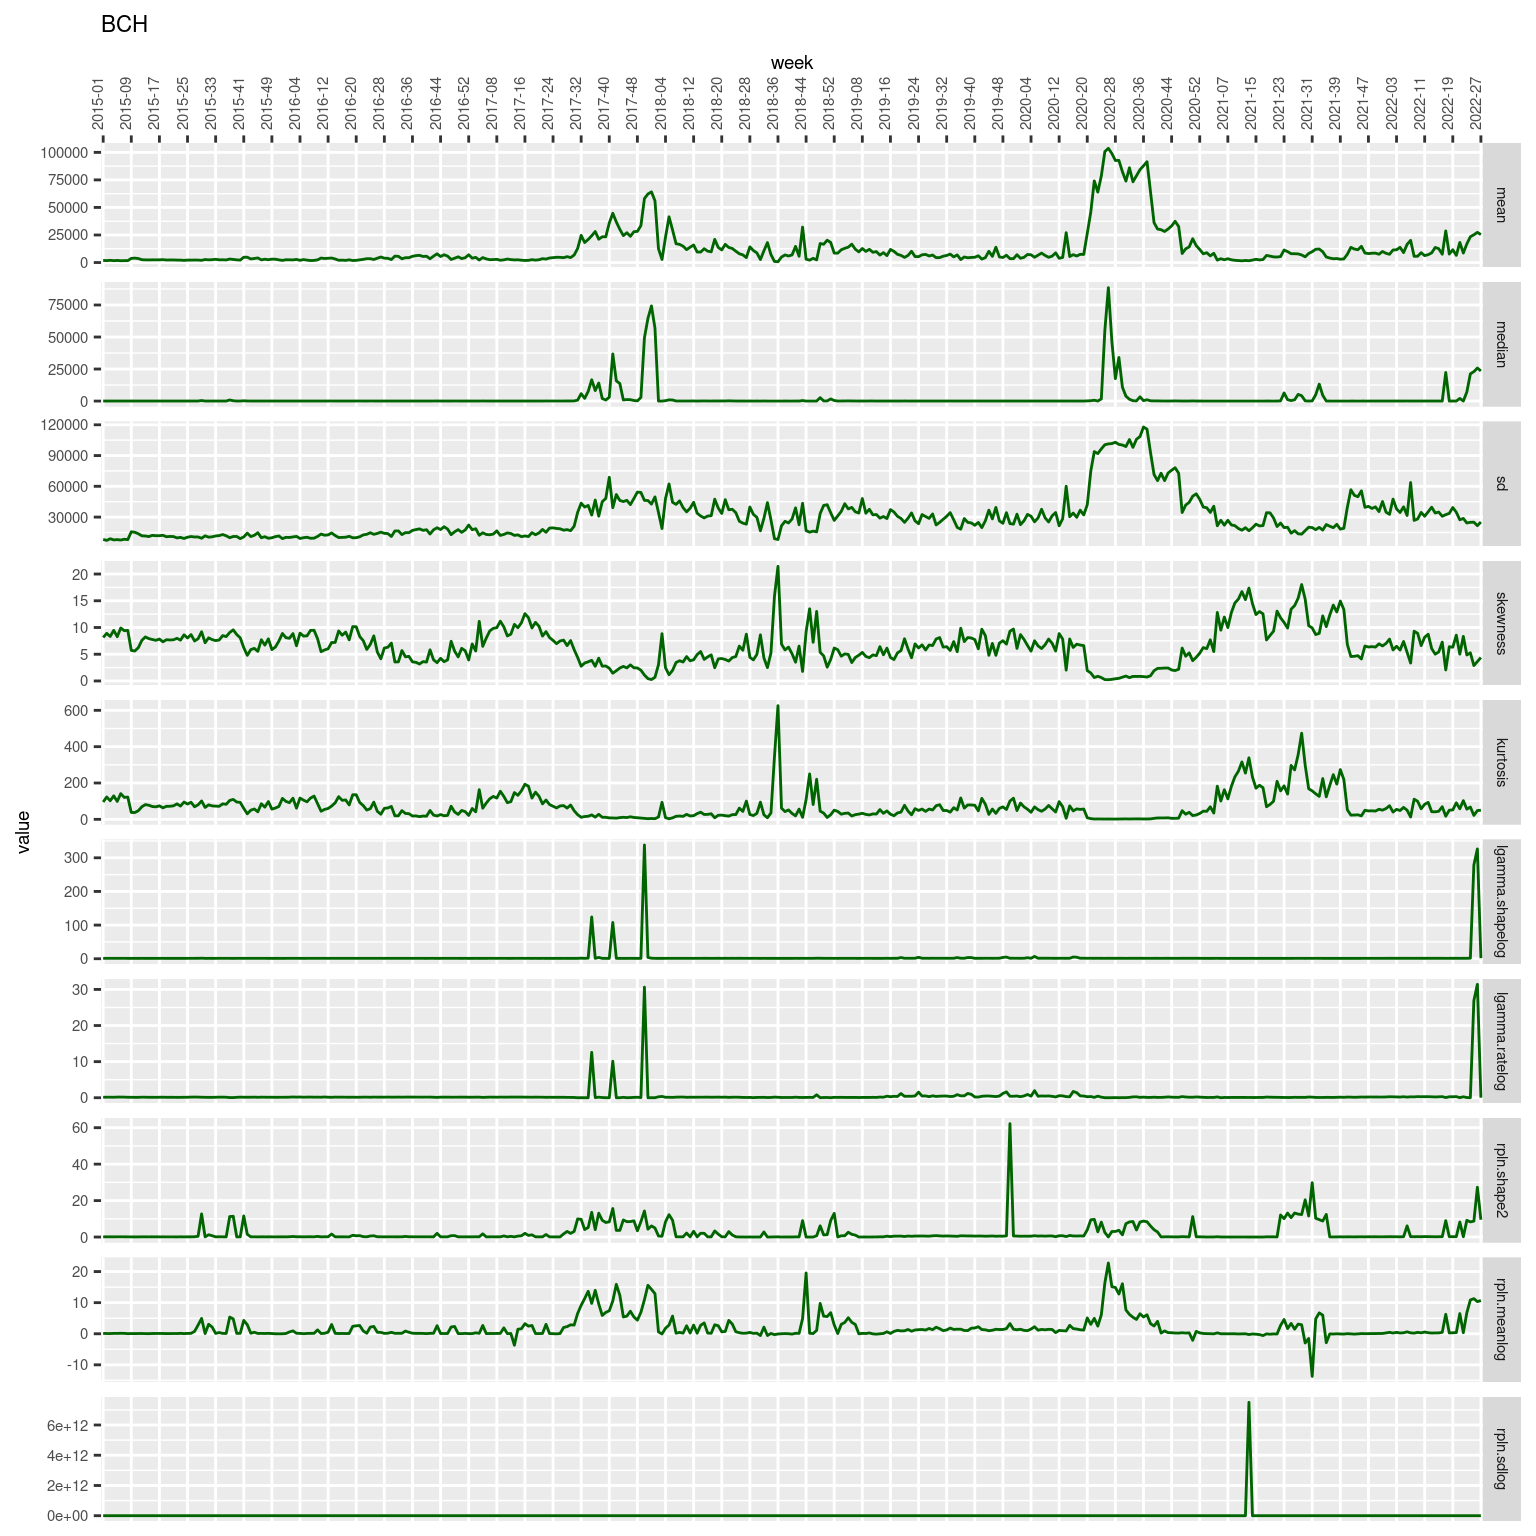
\includegraphics[scale=0.9]{images/spend-age-summary-BCH}
\end{figure}

\begin{figure}[H]
\caption{LTC Summary Characterization of Spend Age Distribution Over Time}

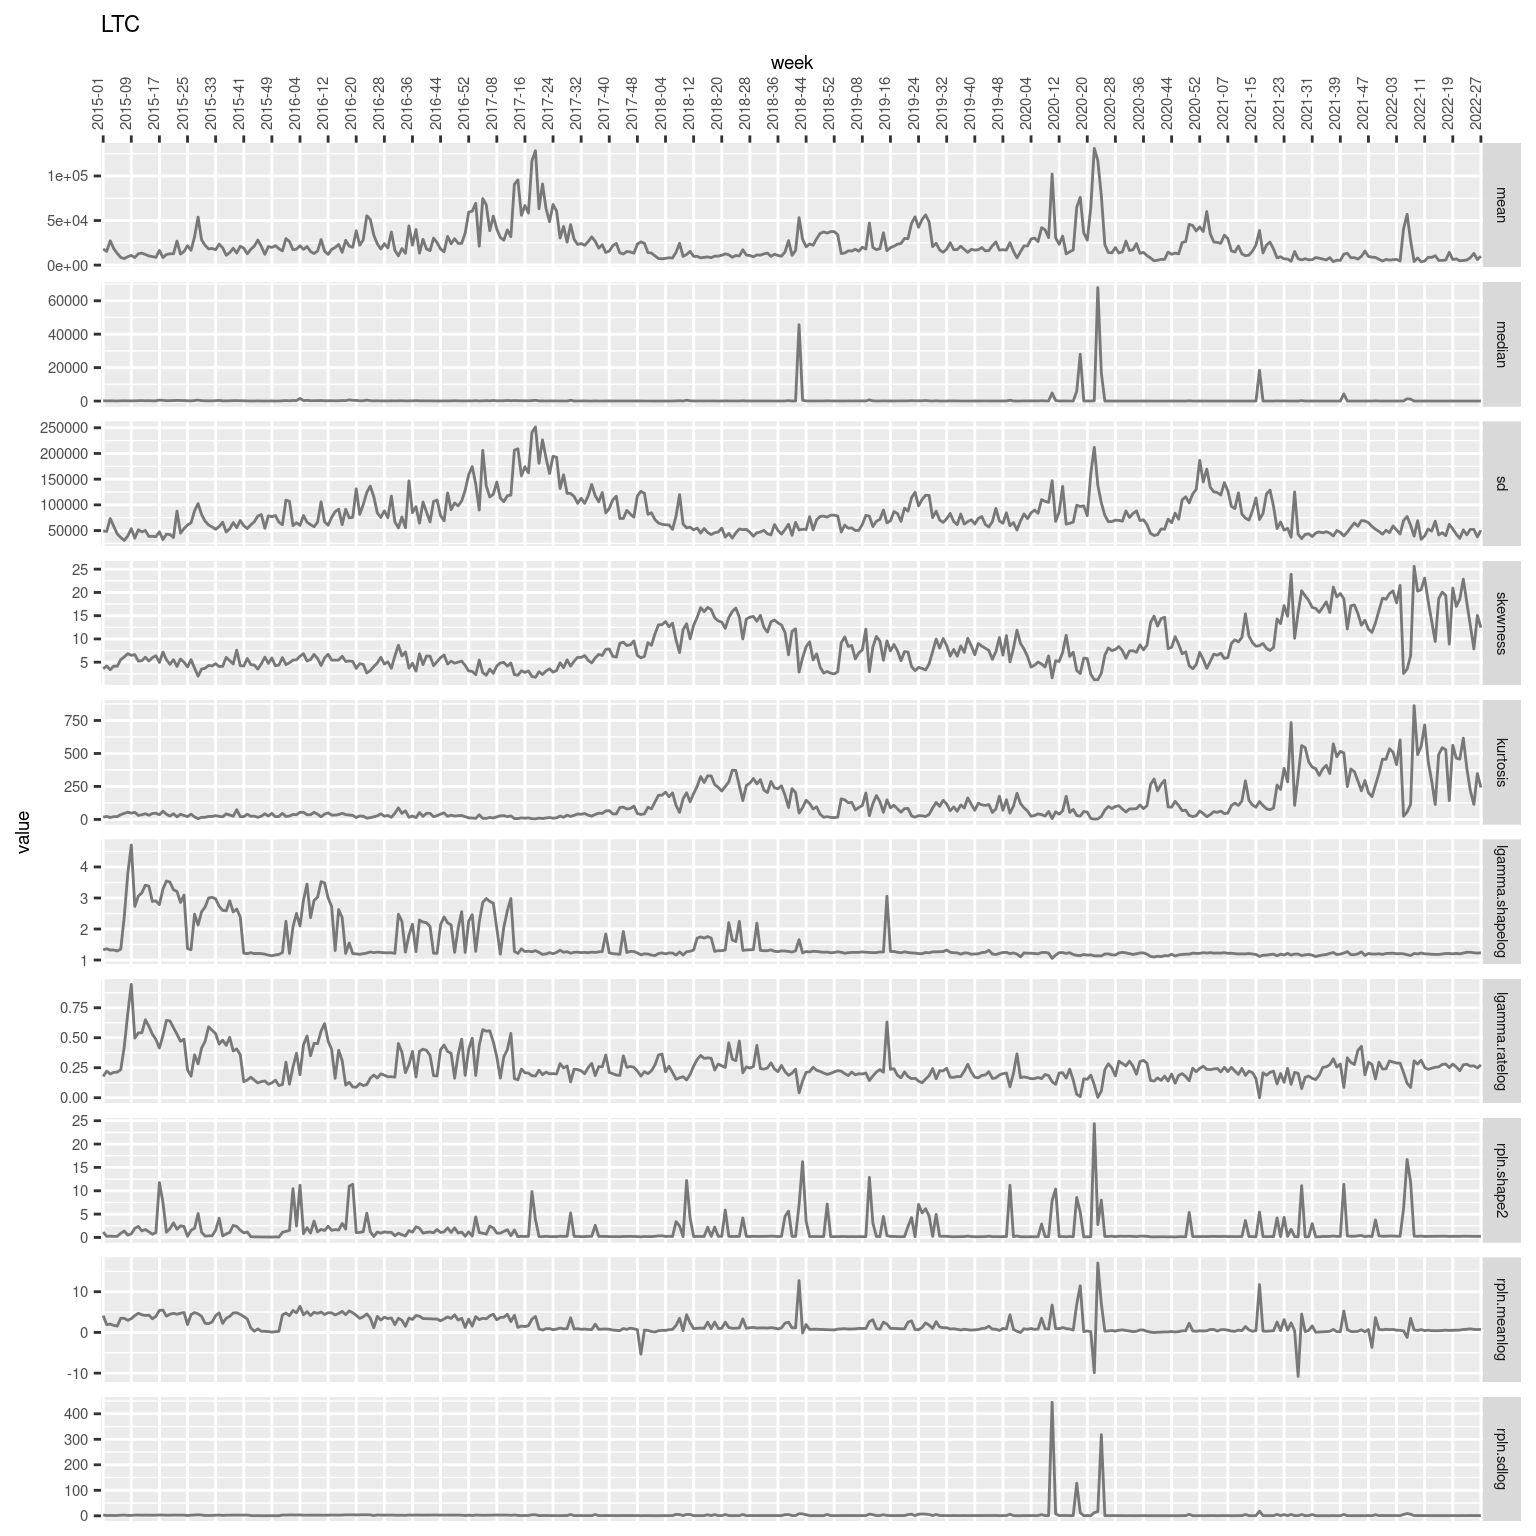
\includegraphics[scale=0.9]{images/spend-age-summary-LTC}
\end{figure}

\begin{figure}[H]
\caption{DOGE Summary Characterization of Spend Age Distribution Over Time}
\label{figure-DOGE-Summary-Characterization}

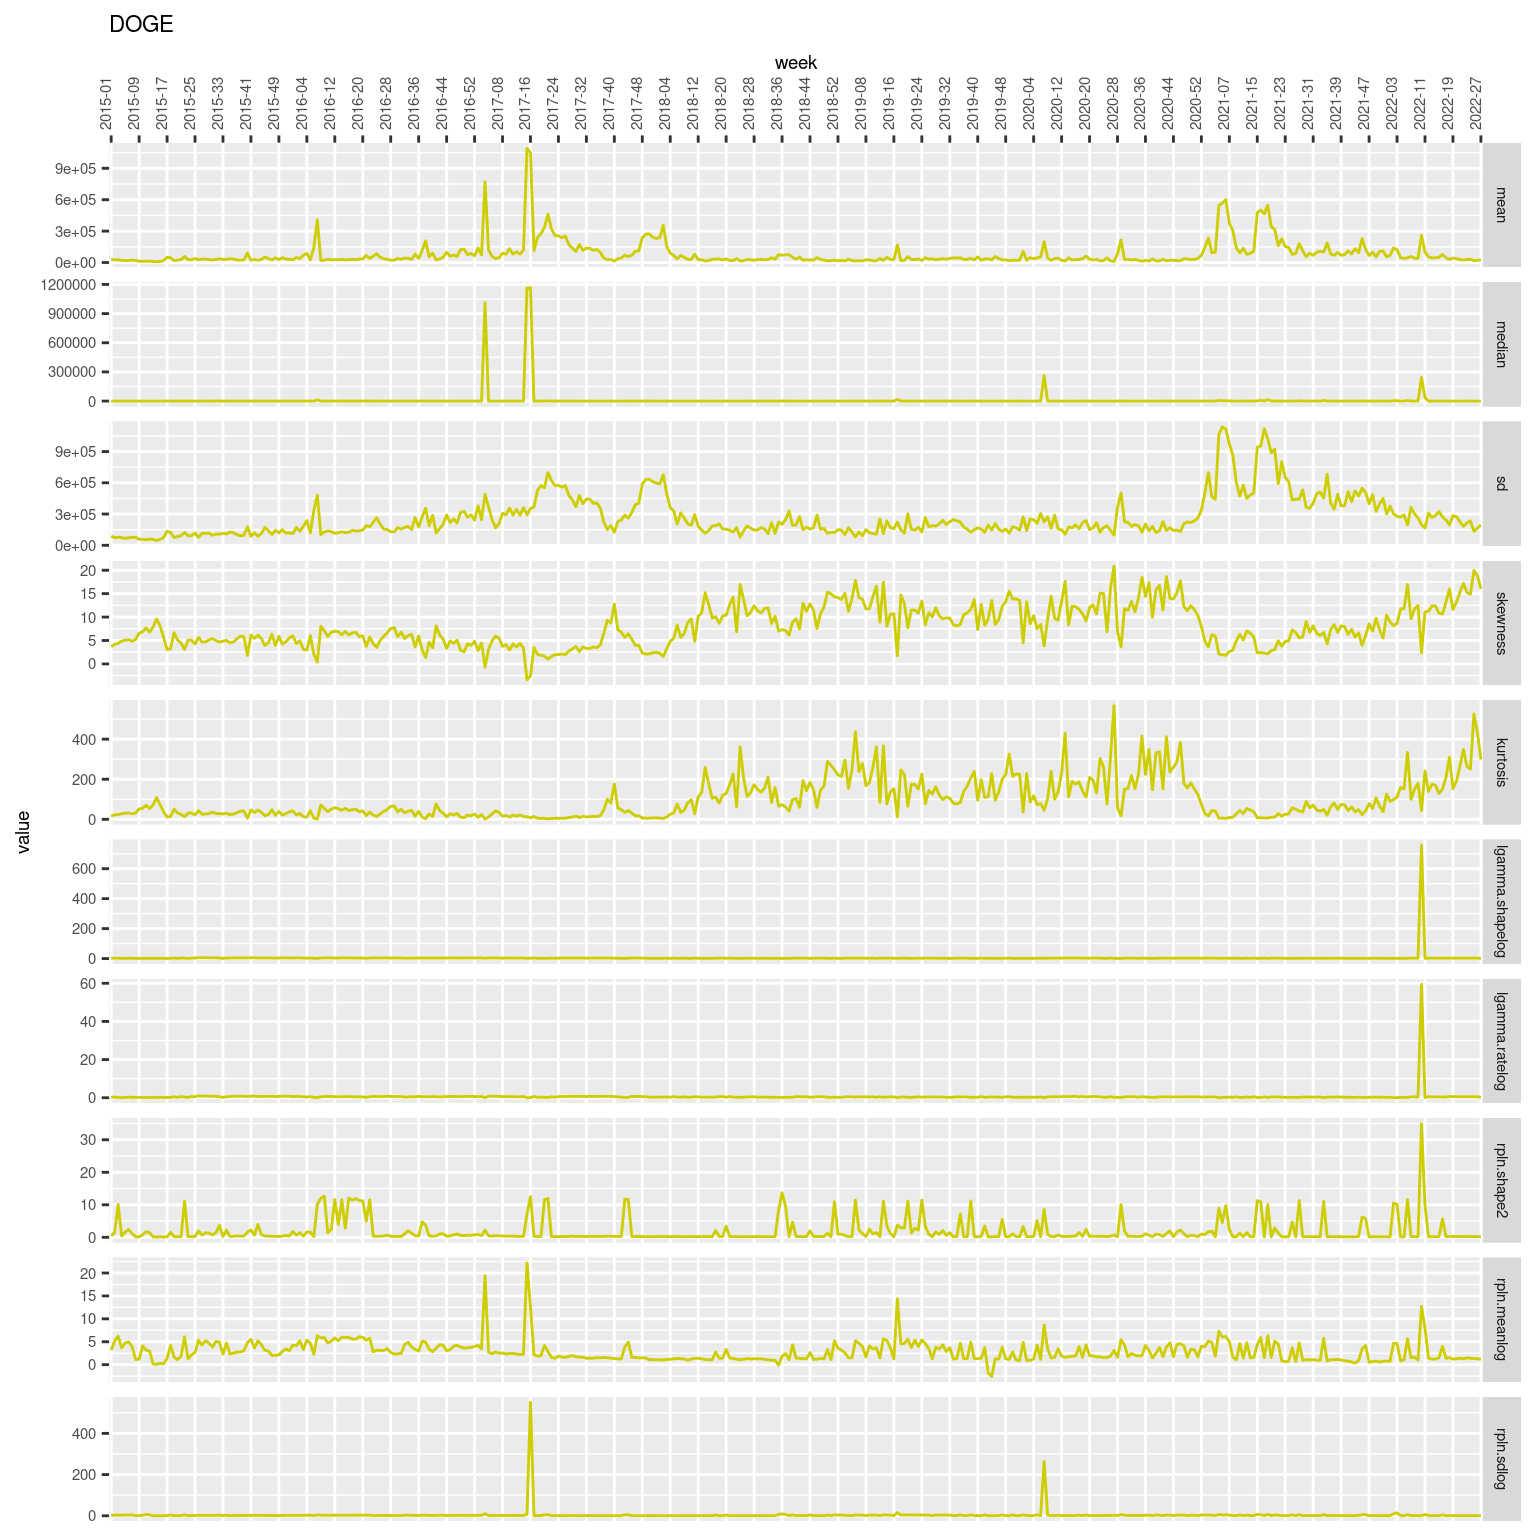
\includegraphics[scale=0.9]{images/spend-age-summary-DOGE}
\end{figure}


\subsection{Cross-Blockchain Correlations of Summary Statistics Across Time}

The following table contains the correlation between several statistics
over time for each pair of blockchains. The ``BTC\&BCH'' correlation
included data only for January 2018 onward to avoid artificially raising
the correlation by including weeks when the BTC and BCH contained
the same transaction before the August 2017 hard fork.

To be precise, define vector $[x_{s,1},x_{s,2},\ldots,x_{s,Z}]=\mathbf{X}_{s}$
for statistic $s$, e.g. the median, of blockchain $x$ at each week,
with $Z$ total weeks in the sample. Define $\mathbf{Y}_{s}$ for
blockchain $y$ similarly. Then the quantities displayed in Table
\ref{table-cross-blockchain-correlations} are $corr(\mathbf{X}_{s},\mathbf{Y}_{s})$.

The two statistics that tend to have consistently high correlation
for each pair of blockchains are skewness and kurtosis. 

\begin{table}[H]

\caption{Cross-Blockchain Correlations of Summary Statistics Across Time}

\label{table-cross-blockchain-correlations}


\begin{tabular}{l|r|r|r|r|r|r}
\hline
  & BTC\&BCH & BTC\&LTC & BTC\&DOGE & BCH\&LTC & BCH\&DOGE & LTC\&DOGE\\
\hline
mean & -0.04 & -0.04 & -0.04 & -0.01 & -0.08 & 0.21\\
\hline
median & -0.03 & -0.01 & -0.01 & -0.03 & -0.02 & -0.01\\
\hline
sd & -0.07 & 0.02 & 0.34 & -0.02 & 0.02 & 0.35\\
\hline
skewness & 0.09 & 0.24 & 0.19 & 0.11 & -0.32 & 0.28\\
\hline
kurtosis & 0.02 & 0.29 & 0.31 & 0.22 & -0.26 & 0.23\\
\hline
\end{tabular}

\end{table}


\subsection{Evaluation of Forecast Accuracy\label{subsec:Evaluation-of-Forecast-Accuracy}}

OSPEAD needs to approximate the real spend age  distribution in the
future, not the past. Ideally, the decoy selection algorithm should
mimic the real spend age distribution at the time that each transaction
is made. Since the real spend age distribution is likely changing
over time, some type of forecasting is needed. Here I perform some
simple evaluation of forecasting methods on transparent blockchains.

Let $W$ be the number of weeks in a forecast horizon. It is the approximate
interval of time that a proposed decoy selection algorithm should
aim to be accurate. Let $M$ be the number of weeks in the data sample.
Then a common way to evaluate a forecasting method is to use the first
$M-W$ weeks to fit a forecasting model. Then determine the performance
of the method by forecasting for $W$ weeks into the ``future''
and compare with the actual sample data of the final $W$ weeks. This
is known as out-of-sample validation. For this exercise, I set $W=8$.

An entire distribution needs to be forecast rather than a single value
or a set of values. Forecasting an entire (empirical, nonparametric)
distribution is extremely complex, so here I reduce the magnitude
of the forecasting problem to just the parameters of the fitted parametric
distributions (lgamma and rpln).

As an initial test, the sophisticated forecasting method used here
was a multivariate auto-regressive(1) exogenous inputs state-space
model with a Koopman-Durbin Kalman filter implemented in the \texttt{MARSS}
R package. The forecasting method allows a forecast into each period
in the future. Since the ``S'' in OSPEAD stands for ``Static'',
only one of the forecast periods can be chosen. I chose the 4th forecast
period since it is roughly in the middle of the 8-week forecast horizon.
This forecast is referred to as simply \texttt{forecast.accuracy}
below.

I also evaluated two naive forecasting methods. The first is to use
the parameters of the $M-W$th week, i.e. the last week of the \textquotedbl training
set\textquotedbl , as the forecast. This is called \texttt{forecast.accuracy.naive.final.week}
below. The second naive method (\texttt{forecast.accuracy.naive.horizon.period})
is to use the final $W$ weeks of the training set to fit the specified
lgamma and rpln distributions by minimizing the $L(\boldsymbol{\beta})$
loss function for a set of weeks of data pooled together rather than
a single week.

Given that the loss function $L(\boldsymbol{\beta})$ is not globally
convex in the choice parameters $\boldsymbol{\beta}$, the numerical
optimization algorithm can go ``off the rails'' and settle at a
local rather than global minimum. Such a failure mode is especially
likely if the empirical distribution is unusual or if the starting
values given to the optimization algorithm are far from the global
minimum. Generally, the solution to this problem is to try different
optimization algorithms, determined better starting values, or use
a computationally expensive grid search method. I chose to defer dealing
with the issue to a later stage in the process. For the purposes of
forecasting, I removed any weeks where the estimated parameters of
the parametric distributions were greater than (or less than) five
times the 95th (5th) percentile from the median. For example, this
exclusion step caused the forecast evaluation for BCH to use the 15th
through 24th weeks of 2022 rather than the 20th through 27th week
as for other blockchains.

The results of the forecast evaluation are in Table \ref{table-Evaluation-of-forecast-accuracy}.
Forecasts were evaluated based on the value of their loss function
$L(\boldsymbol{\beta})$ for each out-of-sample week. Lower values
indicate better performance. The minimum possible value is 0 and the
maximum possible value is 1. The color code scales were calculated
separately for each blockchain. Each color claims a value bin of equal
size. Higher values are red, average values are yellow, and low values
are green.

In this preliminary exercise, \texttt{rpln.forecast.accuracy.naive.horizon.period}
appears to have the most consistently good performance across blockchains.

\begin{sidewaystable}[H]
\caption{Evaluation of forecast accuracy}

\label{table-Evaluation-of-forecast-accuracy}

\tiny

BTC


  \providecommand{\huxb}[2]{\arrayrulecolor[RGB]{#1}\global\arrayrulewidth=#2pt}
  \providecommand{\huxvb}[2]{\color[RGB]{#1}\vrule width #2pt}
  \providecommand{\huxtpad}[1]{\rule{0pt}{#1}}
  \providecommand{\huxbpad}[1]{\rule[-#1]{0pt}{#1}}
\begin{tabular}{l l l l l l l l l l l}


\hhline{}
\arrayrulecolor{black}

\multicolumn{1}{!{\huxvb{0, 0, 0}{0}}r!{\huxvb{0, 0, 0}{0}}}{\huxtpad{6pt + 1em}\raggedleft \hspace{6pt} rownames \hspace{6pt}\huxbpad{6pt}} &
\multicolumn{1}{r!{\huxvb{0, 0, 0}{0}}}{\huxtpad{6pt + 1em}\raggedleft \hspace{6pt} mean \hspace{6pt}\huxbpad{6pt}} &
\multicolumn{1}{r!{\huxvb{0, 0, 0}{0}}}{\huxtpad{6pt + 1em}\raggedleft \hspace{6pt} sd \hspace{6pt}\huxbpad{6pt}} &
\multicolumn{1}{r!{\huxvb{0, 0, 0}{0}}}{\huxtpad{6pt + 1em}\raggedleft \hspace{6pt} 2022-20 \hspace{6pt}\huxbpad{6pt}} &
\multicolumn{1}{r!{\huxvb{0, 0, 0}{0}}}{\huxtpad{6pt + 1em}\raggedleft \hspace{6pt} 2022-21 \hspace{6pt}\huxbpad{6pt}} &
\multicolumn{1}{r!{\huxvb{0, 0, 0}{0}}}{\huxtpad{6pt + 1em}\raggedleft \hspace{6pt} 2022-22 \hspace{6pt}\huxbpad{6pt}} &
\multicolumn{1}{r!{\huxvb{0, 0, 0}{0}}}{\huxtpad{6pt + 1em}\raggedleft \hspace{6pt} 2022-23 \hspace{6pt}\huxbpad{6pt}} &
\multicolumn{1}{r!{\huxvb{0, 0, 0}{0}}}{\huxtpad{6pt + 1em}\raggedleft \hspace{6pt} 2022-24 \hspace{6pt}\huxbpad{6pt}} &
\multicolumn{1}{r!{\huxvb{0, 0, 0}{0}}}{\huxtpad{6pt + 1em}\raggedleft \hspace{6pt} 2022-25 \hspace{6pt}\huxbpad{6pt}} &
\multicolumn{1}{r!{\huxvb{0, 0, 0}{0}}}{\huxtpad{6pt + 1em}\raggedleft \hspace{6pt} 2022-26 \hspace{6pt}\huxbpad{6pt}} &
\multicolumn{1}{l!{\huxvb{0, 0, 0}{0}}}{\huxtpad{6pt + 1em}\raggedright \hspace{6pt} 2022-27 \hspace{6pt}\huxbpad{6pt}} \tabularnewline[-0.5pt]


\hhline{}
\arrayrulecolor{black}

\multicolumn{1}{!{\huxvb{0, 0, 0}{0}}r!{\huxvb{0, 0, 0}{0}}}{\huxtpad{6pt + 1em}\raggedleft \hspace{6pt} rpln.forecast.accuracy \hspace{6pt}\huxbpad{6pt}} &
\multicolumn{1}{r!{\huxvb{0, 0, 0}{0}}}{\cellcolor[RGB]{255, 255, 191}\huxtpad{6pt + 1em}\raggedleft \hspace{6pt} 0.1225 \hspace{6pt}\huxbpad{6pt}} &
\multicolumn{1}{r!{\huxvb{0, 0, 0}{0}}}{\huxtpad{6pt + 1em}\raggedleft \hspace{6pt} 0.0294 \hspace{6pt}\huxbpad{6pt}} &
\multicolumn{1}{r!{\huxvb{0, 0, 0}{0}}}{\cellcolor[RGB]{166, 217, 106}\huxtpad{6pt + 1em}\raggedleft \hspace{6pt} 0.0952 \hspace{6pt}\huxbpad{6pt}} &
\multicolumn{1}{r!{\huxvb{0, 0, 0}{0}}}{\cellcolor[RGB]{217, 239, 139}\huxtpad{6pt + 1em}\raggedleft \hspace{6pt} 0.1086 \hspace{6pt}\huxbpad{6pt}} &
\multicolumn{1}{r!{\huxvb{0, 0, 0}{0}}}{\cellcolor[RGB]{217, 239, 139}\huxtpad{6pt + 1em}\raggedleft \hspace{6pt} 0.1058 \hspace{6pt}\huxbpad{6pt}} &
\multicolumn{1}{r!{\huxvb{0, 0, 0}{0}}}{\cellcolor[RGB]{255, 255, 191}\huxtpad{6pt + 1em}\raggedleft \hspace{6pt} 0.1227 \hspace{6pt}\huxbpad{6pt}} &
\multicolumn{1}{r!{\huxvb{0, 0, 0}{0}}}{\cellcolor[RGB]{166, 217, 106}\huxtpad{6pt + 1em}\raggedleft \hspace{6pt} 0.0926 \hspace{6pt}\huxbpad{6pt}} &
\multicolumn{1}{r!{\huxvb{0, 0, 0}{0}}}{\cellcolor[RGB]{215, 48, 39}\huxtpad{6pt + 1em}\raggedleft \hspace{6pt} 0.1814 \hspace{6pt}\huxbpad{6pt}} &
\multicolumn{1}{r!{\huxvb{0, 0, 0}{0}}}{\cellcolor[RGB]{254, 224, 139}\huxtpad{6pt + 1em}\raggedleft \hspace{6pt} 0.1319 \hspace{6pt}\huxbpad{6pt}} &
\multicolumn{1}{l!{\huxvb{0, 0, 0}{0}}}{\cellcolor[RGB]{254, 224, 139}\huxtpad{6pt + 1em}\raggedright \hspace{6pt} 0.1421 \hspace{6pt}\huxbpad{6pt}} \tabularnewline[-0.5pt]


\hhline{}
\arrayrulecolor{black}

\multicolumn{1}{!{\huxvb{0, 0, 0}{0}}r!{\huxvb{0, 0, 0}{0}}}{\huxtpad{6pt + 1em}\raggedleft \hspace{6pt} rpln.forecast.accuracy.naive.final.week\hphantom{0}\hphantom{0}\hphantom{0}\hphantom{0} \hspace{6pt}\huxbpad{6pt}} &
\multicolumn{1}{r!{\huxvb{0, 0, 0}{0}}}{\cellcolor[RGB]{255, 255, 191}\huxtpad{6pt + 1em}\raggedleft \hspace{6pt} 0.1213 \hspace{6pt}\huxbpad{6pt}} &
\multicolumn{1}{r!{\huxvb{0, 0, 0}{0}}}{\huxtpad{6pt + 1em}\raggedleft \hspace{6pt} 0.0295 \hspace{6pt}\huxbpad{6pt}} &
\multicolumn{1}{r!{\huxvb{0, 0, 0}{0}}}{\cellcolor[RGB]{166, 217, 106}\huxtpad{6pt + 1em}\raggedleft \hspace{6pt} 0.0951 \hspace{6pt}\huxbpad{6pt}} &
\multicolumn{1}{r!{\huxvb{0, 0, 0}{0}}}{\cellcolor[RGB]{217, 239, 139}\huxtpad{6pt + 1em}\raggedleft \hspace{6pt} 0.1068 \hspace{6pt}\huxbpad{6pt}} &
\multicolumn{1}{r!{\huxvb{0, 0, 0}{0}}}{\cellcolor[RGB]{166, 217, 106}\huxtpad{6pt + 1em}\raggedleft \hspace{6pt} 0.1037 \hspace{6pt}\huxbpad{6pt}} &
\multicolumn{1}{r!{\huxvb{0, 0, 0}{0}}}{\cellcolor[RGB]{255, 255, 191}\huxtpad{6pt + 1em}\raggedleft \hspace{6pt} 0.1222 \hspace{6pt}\huxbpad{6pt}} &
\multicolumn{1}{r!{\huxvb{0, 0, 0}{0}}}{\cellcolor[RGB]{166, 217, 106}\huxtpad{6pt + 1em}\raggedleft \hspace{6pt} 0.0910 \hspace{6pt}\huxbpad{6pt}} &
\multicolumn{1}{r!{\huxvb{0, 0, 0}{0}}}{\cellcolor[RGB]{215, 48, 39}\huxtpad{6pt + 1em}\raggedleft \hspace{6pt} 0.1807 \hspace{6pt}\huxbpad{6pt}} &
\multicolumn{1}{r!{\huxvb{0, 0, 0}{0}}}{\cellcolor[RGB]{255, 255, 191}\huxtpad{6pt + 1em}\raggedleft \hspace{6pt} 0.1313 \hspace{6pt}\huxbpad{6pt}} &
\multicolumn{1}{l!{\huxvb{0, 0, 0}{0}}}{\cellcolor[RGB]{254, 224, 139}\huxtpad{6pt + 1em}\raggedright \hspace{6pt} 0.1397 \hspace{6pt}\huxbpad{6pt}} \tabularnewline[-0.5pt]


\hhline{}
\arrayrulecolor{black}

\multicolumn{1}{!{\huxvb{0, 0, 0}{0}}r!{\huxvb{0, 0, 0}{0}}}{\huxtpad{6pt + 1em}\raggedleft \hspace{6pt} rpln.forecast.accuracy.naive.horizon.period\hphantom{0}\hphantom{0} \hspace{6pt}\huxbpad{6pt}} &
\multicolumn{1}{r!{\huxvb{0, 0, 0}{0}}}{\cellcolor[RGB]{26, 152, 80}\huxtpad{6pt + 1em}\raggedleft \hspace{6pt} 0.0682 \hspace{6pt}\huxbpad{6pt}} &
\multicolumn{1}{r!{\huxvb{0, 0, 0}{0}}}{\huxtpad{6pt + 1em}\raggedleft \hspace{6pt} 0.0244 \hspace{6pt}\huxbpad{6pt}} &
\multicolumn{1}{r!{\huxvb{0, 0, 0}{0}}}{\cellcolor[RGB]{102, 189, 99}\huxtpad{6pt + 1em}\raggedleft \hspace{6pt} 0.0795 \hspace{6pt}\huxbpad{6pt}} &
\multicolumn{1}{r!{\huxvb{0, 0, 0}{0}}}{\cellcolor[RGB]{0, 104, 55}\huxtpad{6pt + 1em}\raggedleft \hspace{6pt} 0.0504 \hspace{6pt}\huxbpad{6pt}} &
\multicolumn{1}{r!{\huxvb{0, 0, 0}{0}}}{\cellcolor[RGB]{0, 104, 55}\huxtpad{6pt + 1em}\raggedleft \hspace{6pt} 0.0541 \hspace{6pt}\huxbpad{6pt}} &
\multicolumn{1}{r!{\huxvb{0, 0, 0}{0}}}{\cellcolor[RGB]{0, 104, 55}\huxtpad{6pt + 1em}\raggedleft \hspace{6pt} 0.0601 \hspace{6pt}\huxbpad{6pt}} &
\multicolumn{1}{r!{\huxvb{0, 0, 0}{0}}}{\cellcolor[RGB]{0, 104, 55}\huxtpad{6pt + 1em}\raggedleft \hspace{6pt} 0.0501 \hspace{6pt}\huxbpad{6pt}} &
\multicolumn{1}{r!{\huxvb{0, 0, 0}{0}}}{\cellcolor[RGB]{255, 255, 191}\huxtpad{6pt + 1em}\raggedleft \hspace{6pt} 0.1237 \hspace{6pt}\huxbpad{6pt}} &
\multicolumn{1}{r!{\huxvb{0, 0, 0}{0}}}{\cellcolor[RGB]{26, 152, 80}\huxtpad{6pt + 1em}\raggedleft \hspace{6pt} 0.0645 \hspace{6pt}\huxbpad{6pt}} &
\multicolumn{1}{l!{\huxvb{0, 0, 0}{0}}}{\cellcolor[RGB]{0, 104, 55}\huxtpad{6pt + 1em}\raggedright \hspace{6pt} 0.0632 \hspace{6pt}\huxbpad{6pt}} \tabularnewline[-0.5pt]


\hhline{}
\arrayrulecolor{black}

\multicolumn{1}{!{\huxvb{0, 0, 0}{0}}r!{\huxvb{0, 0, 0}{0}}}{\huxtpad{6pt + 1em}\raggedleft \hspace{6pt} lgamma.forecast.accuracy \hspace{6pt}\huxbpad{6pt}} &
\multicolumn{1}{r!{\huxvb{0, 0, 0}{0}}}{\cellcolor[RGB]{255, 255, 191}\huxtpad{6pt + 1em}\raggedleft \hspace{6pt} 0.1256 \hspace{6pt}\huxbpad{6pt}} &
\multicolumn{1}{r!{\huxvb{0, 0, 0}{0}}}{\huxtpad{6pt + 1em}\raggedleft \hspace{6pt} 0.0215 \hspace{6pt}\huxbpad{6pt}} &
\multicolumn{1}{r!{\huxvb{0, 0, 0}{0}}}{\cellcolor[RGB]{255, 255, 191}\huxtpad{6pt + 1em}\raggedleft \hspace{6pt} 0.1216 \hspace{6pt}\huxbpad{6pt}} &
\multicolumn{1}{r!{\huxvb{0, 0, 0}{0}}}{\cellcolor[RGB]{217, 239, 139}\huxtpad{6pt + 1em}\raggedleft \hspace{6pt} 0.1103 \hspace{6pt}\huxbpad{6pt}} &
\multicolumn{1}{r!{\huxvb{0, 0, 0}{0}}}{\cellcolor[RGB]{217, 239, 139}\huxtpad{6pt + 1em}\raggedleft \hspace{6pt} 0.1151 \hspace{6pt}\huxbpad{6pt}} &
\multicolumn{1}{r!{\huxvb{0, 0, 0}{0}}}{\cellcolor[RGB]{217, 239, 139}\huxtpad{6pt + 1em}\raggedleft \hspace{6pt} 0.1149 \hspace{6pt}\huxbpad{6pt}} &
\multicolumn{1}{r!{\huxvb{0, 0, 0}{0}}}{\cellcolor[RGB]{217, 239, 139}\huxtpad{6pt + 1em}\raggedleft \hspace{6pt} 0.1059 \hspace{6pt}\huxbpad{6pt}} &
\multicolumn{1}{r!{\huxvb{0, 0, 0}{0}}}{\cellcolor[RGB]{215, 48, 39}\huxtpad{6pt + 1em}\raggedleft \hspace{6pt} 0.1733 \hspace{6pt}\huxbpad{6pt}} &
\multicolumn{1}{r!{\huxvb{0, 0, 0}{0}}}{\cellcolor[RGB]{255, 255, 191}\huxtpad{6pt + 1em}\raggedleft \hspace{6pt} 0.1299 \hspace{6pt}\huxbpad{6pt}} &
\multicolumn{1}{l!{\huxvb{0, 0, 0}{0}}}{\cellcolor[RGB]{254, 224, 139}\huxtpad{6pt + 1em}\raggedright \hspace{6pt} 0.1341 \hspace{6pt}\huxbpad{6pt}} \tabularnewline[-0.5pt]


\hhline{}
\arrayrulecolor{black}

\multicolumn{1}{!{\huxvb{0, 0, 0}{0}}r!{\huxvb{0, 0, 0}{0}}}{\huxtpad{6pt + 1em}\raggedleft \hspace{6pt} lgamma.forecast.accuracy.naive.final.week\hphantom{0}\hphantom{0}\hphantom{0}\hphantom{0} \hspace{6pt}\huxbpad{6pt}} &
\multicolumn{1}{r!{\huxvb{0, 0, 0}{0}}}{\cellcolor[RGB]{253, 174, 97}\huxtpad{6pt + 1em}\raggedleft \hspace{6pt} 0.1495 \hspace{6pt}\huxbpad{6pt}} &
\multicolumn{1}{r!{\huxvb{0, 0, 0}{0}}}{\huxtpad{6pt + 1em}\raggedleft \hspace{6pt} 0.0277 \hspace{6pt}\huxbpad{6pt}} &
\multicolumn{1}{r!{\huxvb{0, 0, 0}{0}}}{\cellcolor[RGB]{217, 239, 139}\huxtpad{6pt + 1em}\raggedleft \hspace{6pt} 0.1179 \hspace{6pt}\huxbpad{6pt}} &
\multicolumn{1}{r!{\huxvb{0, 0, 0}{0}}}{\cellcolor[RGB]{254, 224, 139}\huxtpad{6pt + 1em}\raggedleft \hspace{6pt} 0.1373 \hspace{6pt}\huxbpad{6pt}} &
\multicolumn{1}{r!{\huxvb{0, 0, 0}{0}}}{\cellcolor[RGB]{254, 224, 139}\huxtpad{6pt + 1em}\raggedleft \hspace{6pt} 0.1373 \hspace{6pt}\huxbpad{6pt}} &
\multicolumn{1}{r!{\huxvb{0, 0, 0}{0}}}{\cellcolor[RGB]{253, 174, 97}\huxtpad{6pt + 1em}\raggedleft \hspace{6pt} 0.1519 \hspace{6pt}\huxbpad{6pt}} &
\multicolumn{1}{r!{\huxvb{0, 0, 0}{0}}}{\cellcolor[RGB]{255, 255, 191}\huxtpad{6pt + 1em}\raggedleft \hspace{6pt} 0.1188 \hspace{6pt}\huxbpad{6pt}} &
\multicolumn{1}{r!{\huxvb{0, 0, 0}{0}}}{\cellcolor[RGB]{165, 0, 38}\huxtpad{6pt + 1em}\raggedleft \hspace{6pt} 0.1996 \hspace{6pt}\huxbpad{6pt}} &
\multicolumn{1}{r!{\huxvb{0, 0, 0}{0}}}{\cellcolor[RGB]{244, 109, 67}\huxtpad{6pt + 1em}\raggedleft \hspace{6pt} 0.1613 \hspace{6pt}\huxbpad{6pt}} &
\multicolumn{1}{l!{\huxvb{0, 0, 0}{0}}}{\cellcolor[RGB]{244, 109, 67}\huxtpad{6pt + 1em}\raggedright \hspace{6pt} 0.1717 \hspace{6pt}\huxbpad{6pt}} \tabularnewline[-0.5pt]


\hhline{}
\arrayrulecolor{black}

\multicolumn{1}{!{\huxvb{0, 0, 0}{0}}r!{\huxvb{0, 0, 0}{0}}}{\huxtpad{6pt + 1em}\raggedleft \hspace{6pt} lgamma.forecast.accuracy.naive.horizon.period\hphantom{0}\hphantom{0} \hspace{6pt}\huxbpad{6pt}} &
\multicolumn{1}{r!{\huxvb{0, 0, 0}{0}}}{\cellcolor[RGB]{254, 224, 139}\huxtpad{6pt + 1em}\raggedleft \hspace{6pt} 0.1338 \hspace{6pt}\huxbpad{6pt}} &
\multicolumn{1}{r!{\huxvb{0, 0, 0}{0}}}{\huxtpad{6pt + 1em}\raggedleft \hspace{6pt} 0.0177 \hspace{6pt}\huxbpad{6pt}} &
\multicolumn{1}{r!{\huxvb{0, 0, 0}{0}}}{\cellcolor[RGB]{255, 255, 191}\huxtpad{6pt + 1em}\raggedleft \hspace{6pt} 0.1302 \hspace{6pt}\huxbpad{6pt}} &
\multicolumn{1}{r!{\huxvb{0, 0, 0}{0}}}{\cellcolor[RGB]{255, 255, 191}\huxtpad{6pt + 1em}\raggedleft \hspace{6pt} 0.1183 \hspace{6pt}\huxbpad{6pt}} &
\multicolumn{1}{r!{\huxvb{0, 0, 0}{0}}}{\cellcolor[RGB]{255, 255, 191}\huxtpad{6pt + 1em}\raggedleft \hspace{6pt} 0.1274 \hspace{6pt}\huxbpad{6pt}} &
\multicolumn{1}{r!{\huxvb{0, 0, 0}{0}}}{\cellcolor[RGB]{255, 255, 191}\huxtpad{6pt + 1em}\raggedleft \hspace{6pt} 0.1212 \hspace{6pt}\huxbpad{6pt}} &
\multicolumn{1}{r!{\huxvb{0, 0, 0}{0}}}{\cellcolor[RGB]{255, 255, 191}\huxtpad{6pt + 1em}\raggedleft \hspace{6pt} 0.1205 \hspace{6pt}\huxbpad{6pt}} &
\multicolumn{1}{r!{\huxvb{0, 0, 0}{0}}}{\cellcolor[RGB]{244, 109, 67}\huxtpad{6pt + 1em}\raggedleft \hspace{6pt} 0.1716 \hspace{6pt}\huxbpad{6pt}} &
\multicolumn{1}{r!{\huxvb{0, 0, 0}{0}}}{\cellcolor[RGB]{254, 224, 139}\huxtpad{6pt + 1em}\raggedleft \hspace{6pt} 0.1358 \hspace{6pt}\huxbpad{6pt}} &
\multicolumn{1}{l!{\huxvb{0, 0, 0}{0}}}{\cellcolor[RGB]{253, 174, 97}\huxtpad{6pt + 1em}\raggedright \hspace{6pt} 0.1453 \hspace{6pt}\huxbpad{6pt}} \tabularnewline[-0.5pt]


\hhline{}
\arrayrulecolor{black}
\end{tabular}


BCH


  \providecommand{\huxb}[2]{\arrayrulecolor[RGB]{#1}\global\arrayrulewidth=#2pt}
  \providecommand{\huxvb}[2]{\color[RGB]{#1}\vrule width #2pt}
  \providecommand{\huxtpad}[1]{\rule{0pt}{#1}}
  \providecommand{\huxbpad}[1]{\rule[-#1]{0pt}{#1}}
\begin{tabular}{l l l l l l l l l l l}


\hhline{}
\arrayrulecolor{black}

\multicolumn{1}{!{\huxvb{0, 0, 0}{0}}r!{\huxvb{0, 0, 0}{0}}}{\huxtpad{6pt + 1em}\raggedleft \hspace{6pt} rownames \hspace{6pt}\huxbpad{6pt}} &
\multicolumn{1}{r!{\huxvb{0, 0, 0}{0}}}{\huxtpad{6pt + 1em}\raggedleft \hspace{6pt} mean \hspace{6pt}\huxbpad{6pt}} &
\multicolumn{1}{r!{\huxvb{0, 0, 0}{0}}}{\huxtpad{6pt + 1em}\raggedleft \hspace{6pt} sd \hspace{6pt}\huxbpad{6pt}} &
\multicolumn{1}{r!{\huxvb{0, 0, 0}{0}}}{\huxtpad{6pt + 1em}\raggedleft \hspace{6pt} 2022-15 \hspace{6pt}\huxbpad{6pt}} &
\multicolumn{1}{r!{\huxvb{0, 0, 0}{0}}}{\huxtpad{6pt + 1em}\raggedleft \hspace{6pt} 2022-16 \hspace{6pt}\huxbpad{6pt}} &
\multicolumn{1}{r!{\huxvb{0, 0, 0}{0}}}{\huxtpad{6pt + 1em}\raggedleft \hspace{6pt} 2022-18 \hspace{6pt}\huxbpad{6pt}} &
\multicolumn{1}{r!{\huxvb{0, 0, 0}{0}}}{\huxtpad{6pt + 1em}\raggedleft \hspace{6pt} 2022-19 \hspace{6pt}\huxbpad{6pt}} &
\multicolumn{1}{r!{\huxvb{0, 0, 0}{0}}}{\huxtpad{6pt + 1em}\raggedleft \hspace{6pt} 2022-20 \hspace{6pt}\huxbpad{6pt}} &
\multicolumn{1}{r!{\huxvb{0, 0, 0}{0}}}{\huxtpad{6pt + 1em}\raggedleft \hspace{6pt} 2022-21 \hspace{6pt}\huxbpad{6pt}} &
\multicolumn{1}{r!{\huxvb{0, 0, 0}{0}}}{\huxtpad{6pt + 1em}\raggedleft \hspace{6pt} 2022-22 \hspace{6pt}\huxbpad{6pt}} &
\multicolumn{1}{l!{\huxvb{0, 0, 0}{0}}}{\huxtpad{6pt + 1em}\raggedright \hspace{6pt} 2022-24 \hspace{6pt}\huxbpad{6pt}} \tabularnewline[-0.5pt]


\hhline{}
\arrayrulecolor{black}

\multicolumn{1}{!{\huxvb{0, 0, 0}{0}}r!{\huxvb{0, 0, 0}{0}}}{\huxtpad{6pt + 1em}\raggedleft \hspace{6pt} rpln.forecast.accuracy \hspace{6pt}\huxbpad{6pt}} &
\multicolumn{1}{r!{\huxvb{0, 0, 0}{0}}}{\cellcolor[RGB]{102, 189, 99}\huxtpad{6pt + 1em}\raggedleft \hspace{6pt} 0.2416 \hspace{6pt}\huxbpad{6pt}} &
\multicolumn{1}{r!{\huxvb{0, 0, 0}{0}}}{\huxtpad{6pt + 1em}\raggedleft \hspace{6pt} 0.1923 \hspace{6pt}\huxbpad{6pt}} &
\multicolumn{1}{r!{\huxvb{0, 0, 0}{0}}}{\cellcolor[RGB]{26, 152, 80}\huxtpad{6pt + 1em}\raggedleft \hspace{6pt} 0.1811 \hspace{6pt}\huxbpad{6pt}} &
\multicolumn{1}{r!{\huxvb{0, 0, 0}{0}}}{\cellcolor[RGB]{0, 104, 55}\huxtpad{6pt + 1em}\raggedleft \hspace{6pt} 0.1420 \hspace{6pt}\huxbpad{6pt}} &
\multicolumn{1}{r!{\huxvb{0, 0, 0}{0}}}{\cellcolor[RGB]{0, 104, 55}\huxtpad{6pt + 1em}\raggedleft \hspace{6pt} 0.1147 \hspace{6pt}\huxbpad{6pt}} &
\multicolumn{1}{r!{\huxvb{0, 0, 0}{0}}}{\cellcolor[RGB]{26, 152, 80}\huxtpad{6pt + 1em}\raggedleft \hspace{6pt} 0.1598 \hspace{6pt}\huxbpad{6pt}} &
\multicolumn{1}{r!{\huxvb{0, 0, 0}{0}}}{\cellcolor[RGB]{0, 104, 55}\huxtpad{6pt + 1em}\raggedleft \hspace{6pt} 0.1057 \hspace{6pt}\huxbpad{6pt}} &
\multicolumn{1}{r!{\huxvb{0, 0, 0}{0}}}{\cellcolor[RGB]{254, 224, 139}\huxtpad{6pt + 1em}\raggedleft \hspace{6pt} 0.4079 \hspace{6pt}\huxbpad{6pt}} &
\multicolumn{1}{r!{\huxvb{0, 0, 0}{0}}}{\cellcolor[RGB]{26, 152, 80}\huxtpad{6pt + 1em}\raggedleft \hspace{6pt} 0.1665 \hspace{6pt}\huxbpad{6pt}} &
\multicolumn{1}{l!{\huxvb{0, 0, 0}{0}}}{\cellcolor[RGB]{165, 0, 38}\huxtpad{6pt + 1em}\raggedright \hspace{6pt} 0.6547 \hspace{6pt}\huxbpad{6pt}} \tabularnewline[-0.5pt]


\hhline{}
\arrayrulecolor{black}

\multicolumn{1}{!{\huxvb{0, 0, 0}{0}}r!{\huxvb{0, 0, 0}{0}}}{\huxtpad{6pt + 1em}\raggedleft \hspace{6pt} rpln.forecast.accuracy.naive.final.week\hphantom{0}\hphantom{0}\hphantom{0}\hphantom{0} \hspace{6pt}\huxbpad{6pt}} &
\multicolumn{1}{r!{\huxvb{0, 0, 0}{0}}}{\cellcolor[RGB]{102, 189, 99}\huxtpad{6pt + 1em}\raggedleft \hspace{6pt} 0.2452 \hspace{6pt}\huxbpad{6pt}} &
\multicolumn{1}{r!{\huxvb{0, 0, 0}{0}}}{\huxtpad{6pt + 1em}\raggedleft \hspace{6pt} 0.1808 \hspace{6pt}\huxbpad{6pt}} &
\multicolumn{1}{r!{\huxvb{0, 0, 0}{0}}}{\cellcolor[RGB]{26, 152, 80}\huxtpad{6pt + 1em}\raggedleft \hspace{6pt} 0.1882 \hspace{6pt}\huxbpad{6pt}} &
\multicolumn{1}{r!{\huxvb{0, 0, 0}{0}}}{\cellcolor[RGB]{0, 104, 55}\huxtpad{6pt + 1em}\raggedleft \hspace{6pt} 0.1530 \hspace{6pt}\huxbpad{6pt}} &
\multicolumn{1}{r!{\huxvb{0, 0, 0}{0}}}{\cellcolor[RGB]{0, 104, 55}\huxtpad{6pt + 1em}\raggedleft \hspace{6pt} 0.1302 \hspace{6pt}\huxbpad{6pt}} &
\multicolumn{1}{r!{\huxvb{0, 0, 0}{0}}}{\cellcolor[RGB]{26, 152, 80}\huxtpad{6pt + 1em}\raggedleft \hspace{6pt} 0.1668 \hspace{6pt}\huxbpad{6pt}} &
\multicolumn{1}{r!{\huxvb{0, 0, 0}{0}}}{\cellcolor[RGB]{0, 104, 55}\huxtpad{6pt + 1em}\raggedleft \hspace{6pt} 0.1208 \hspace{6pt}\huxbpad{6pt}} &
\multicolumn{1}{r!{\huxvb{0, 0, 0}{0}}}{\cellcolor[RGB]{255, 255, 191}\huxtpad{6pt + 1em}\raggedleft \hspace{6pt} 0.3957 \hspace{6pt}\huxbpad{6pt}} &
\multicolumn{1}{r!{\huxvb{0, 0, 0}{0}}}{\cellcolor[RGB]{26, 152, 80}\huxtpad{6pt + 1em}\raggedleft \hspace{6pt} 0.1692 \hspace{6pt}\huxbpad{6pt}} &
\multicolumn{1}{l!{\huxvb{0, 0, 0}{0}}}{\cellcolor[RGB]{165, 0, 38}\huxtpad{6pt + 1em}\raggedright \hspace{6pt} 0.6375 \hspace{6pt}\huxbpad{6pt}} \tabularnewline[-0.5pt]


\hhline{}
\arrayrulecolor{black}

\multicolumn{1}{!{\huxvb{0, 0, 0}{0}}r!{\huxvb{0, 0, 0}{0}}}{\huxtpad{6pt + 1em}\raggedleft \hspace{6pt} rpln.forecast.accuracy.naive.horizon.period\hphantom{0}\hphantom{0} \hspace{6pt}\huxbpad{6pt}} &
\multicolumn{1}{r!{\huxvb{0, 0, 0}{0}}}{\cellcolor[RGB]{255, 255, 191}\huxtpad{6pt + 1em}\raggedleft \hspace{6pt} 0.3938 \hspace{6pt}\huxbpad{6pt}} &
\multicolumn{1}{r!{\huxvb{0, 0, 0}{0}}}{\huxtpad{6pt + 1em}\raggedleft \hspace{6pt} 0.0463 \hspace{6pt}\huxbpad{6pt}} &
\multicolumn{1}{r!{\huxvb{0, 0, 0}{0}}}{\cellcolor[RGB]{255, 255, 191}\huxtpad{6pt + 1em}\raggedleft \hspace{6pt} 0.3837 \hspace{6pt}\huxbpad{6pt}} &
\multicolumn{1}{r!{\huxvb{0, 0, 0}{0}}}{\cellcolor[RGB]{255, 255, 191}\huxtpad{6pt + 1em}\raggedleft \hspace{6pt} 0.3886 \hspace{6pt}\huxbpad{6pt}} &
\multicolumn{1}{r!{\huxvb{0, 0, 0}{0}}}{\cellcolor[RGB]{255, 255, 191}\huxtpad{6pt + 1em}\raggedleft \hspace{6pt} 0.3754 \hspace{6pt}\huxbpad{6pt}} &
\multicolumn{1}{r!{\huxvb{0, 0, 0}{0}}}{\cellcolor[RGB]{255, 255, 191}\huxtpad{6pt + 1em}\raggedleft \hspace{6pt} 0.3830 \hspace{6pt}\huxbpad{6pt}} &
\multicolumn{1}{r!{\huxvb{0, 0, 0}{0}}}{\cellcolor[RGB]{255, 255, 191}\huxtpad{6pt + 1em}\raggedleft \hspace{6pt} 0.3809 \hspace{6pt}\huxbpad{6pt}} &
\multicolumn{1}{r!{\huxvb{0, 0, 0}{0}}}{\cellcolor[RGB]{255, 255, 191}\huxtpad{6pt + 1em}\raggedleft \hspace{6pt} 0.3812 \hspace{6pt}\huxbpad{6pt}} &
\multicolumn{1}{r!{\huxvb{0, 0, 0}{0}}}{\cellcolor[RGB]{217, 239, 139}\huxtpad{6pt + 1em}\raggedleft \hspace{6pt} 0.3526 \hspace{6pt}\huxbpad{6pt}} &
\multicolumn{1}{l!{\huxvb{0, 0, 0}{0}}}{\cellcolor[RGB]{244, 109, 67}\huxtpad{6pt + 1em}\raggedright \hspace{6pt} 0.5051 \hspace{6pt}\huxbpad{6pt}} \tabularnewline[-0.5pt]


\hhline{}
\arrayrulecolor{black}

\multicolumn{1}{!{\huxvb{0, 0, 0}{0}}r!{\huxvb{0, 0, 0}{0}}}{\huxtpad{6pt + 1em}\raggedleft \hspace{6pt} lgamma.forecast.accuracy \hspace{6pt}\huxbpad{6pt}} &
\multicolumn{1}{r!{\huxvb{0, 0, 0}{0}}}{\cellcolor[RGB]{255, 255, 191}\huxtpad{6pt + 1em}\raggedleft \hspace{6pt} 0.3654 \hspace{6pt}\huxbpad{6pt}} &
\multicolumn{1}{r!{\huxvb{0, 0, 0}{0}}}{\huxtpad{6pt + 1em}\raggedleft \hspace{6pt} 0.1374 \hspace{6pt}\huxbpad{6pt}} &
\multicolumn{1}{r!{\huxvb{0, 0, 0}{0}}}{\cellcolor[RGB]{166, 217, 106}\huxtpad{6pt + 1em}\raggedleft \hspace{6pt} 0.2606 \hspace{6pt}\huxbpad{6pt}} &
\multicolumn{1}{r!{\huxvb{0, 0, 0}{0}}}{\cellcolor[RGB]{166, 217, 106}\huxtpad{6pt + 1em}\raggedleft \hspace{6pt} 0.2757 \hspace{6pt}\huxbpad{6pt}} &
\multicolumn{1}{r!{\huxvb{0, 0, 0}{0}}}{\cellcolor[RGB]{166, 217, 106}\huxtpad{6pt + 1em}\raggedleft \hspace{6pt} 0.2574 \hspace{6pt}\huxbpad{6pt}} &
\multicolumn{1}{r!{\huxvb{0, 0, 0}{0}}}{\cellcolor[RGB]{217, 239, 139}\huxtpad{6pt + 1em}\raggedleft \hspace{6pt} 0.3479 \hspace{6pt}\huxbpad{6pt}} &
\multicolumn{1}{r!{\huxvb{0, 0, 0}{0}}}{\cellcolor[RGB]{102, 189, 99}\huxtpad{6pt + 1em}\raggedleft \hspace{6pt} 0.2506 \hspace{6pt}\huxbpad{6pt}} &
\multicolumn{1}{r!{\huxvb{0, 0, 0}{0}}}{\cellcolor[RGB]{255, 255, 191}\huxtpad{6pt + 1em}\raggedleft \hspace{6pt} 0.3830 \hspace{6pt}\huxbpad{6pt}} &
\multicolumn{1}{r!{\huxvb{0, 0, 0}{0}}}{\cellcolor[RGB]{215, 48, 39}\huxtpad{6pt + 1em}\raggedleft \hspace{6pt} 0.5578 \hspace{6pt}\huxbpad{6pt}} &
\multicolumn{1}{l!{\huxvb{0, 0, 0}{0}}}{\cellcolor[RGB]{215, 48, 39}\huxtpad{6pt + 1em}\raggedright \hspace{6pt} 0.5906 \hspace{6pt}\huxbpad{6pt}} \tabularnewline[-0.5pt]


\hhline{}
\arrayrulecolor{black}

\multicolumn{1}{!{\huxvb{0, 0, 0}{0}}r!{\huxvb{0, 0, 0}{0}}}{\huxtpad{6pt + 1em}\raggedleft \hspace{6pt} lgamma.forecast.accuracy.naive.final.week\hphantom{0}\hphantom{0}\hphantom{0}\hphantom{0} \hspace{6pt}\huxbpad{6pt}} &
\multicolumn{1}{r!{\huxvb{0, 0, 0}{0}}}{\cellcolor[RGB]{255, 255, 191}\huxtpad{6pt + 1em}\raggedleft \hspace{6pt} 0.3573 \hspace{6pt}\huxbpad{6pt}} &
\multicolumn{1}{r!{\huxvb{0, 0, 0}{0}}}{\huxtpad{6pt + 1em}\raggedleft \hspace{6pt} 0.1491 \hspace{6pt}\huxbpad{6pt}} &
\multicolumn{1}{r!{\huxvb{0, 0, 0}{0}}}{\cellcolor[RGB]{102, 189, 99}\huxtpad{6pt + 1em}\raggedleft \hspace{6pt} 0.2401 \hspace{6pt}\huxbpad{6pt}} &
\multicolumn{1}{r!{\huxvb{0, 0, 0}{0}}}{\cellcolor[RGB]{102, 189, 99}\huxtpad{6pt + 1em}\raggedleft \hspace{6pt} 0.2553 \hspace{6pt}\huxbpad{6pt}} &
\multicolumn{1}{r!{\huxvb{0, 0, 0}{0}}}{\cellcolor[RGB]{102, 189, 99}\huxtpad{6pt + 1em}\raggedleft \hspace{6pt} 0.2367 \hspace{6pt}\huxbpad{6pt}} &
\multicolumn{1}{r!{\huxvb{0, 0, 0}{0}}}{\cellcolor[RGB]{217, 239, 139}\huxtpad{6pt + 1em}\raggedleft \hspace{6pt} 0.3476 \hspace{6pt}\huxbpad{6pt}} &
\multicolumn{1}{r!{\huxvb{0, 0, 0}{0}}}{\cellcolor[RGB]{102, 189, 99}\huxtpad{6pt + 1em}\raggedleft \hspace{6pt} 0.2313 \hspace{6pt}\huxbpad{6pt}} &
\multicolumn{1}{r!{\huxvb{0, 0, 0}{0}}}{\cellcolor[RGB]{255, 255, 191}\huxtpad{6pt + 1em}\raggedleft \hspace{6pt} 0.3867 \hspace{6pt}\huxbpad{6pt}} &
\multicolumn{1}{r!{\huxvb{0, 0, 0}{0}}}{\cellcolor[RGB]{215, 48, 39}\huxtpad{6pt + 1em}\raggedleft \hspace{6pt} 0.5643 \hspace{6pt}\huxbpad{6pt}} &
\multicolumn{1}{l!{\huxvb{0, 0, 0}{0}}}{\cellcolor[RGB]{215, 48, 39}\huxtpad{6pt + 1em}\raggedright \hspace{6pt} 0.5967 \hspace{6pt}\huxbpad{6pt}} \tabularnewline[-0.5pt]


\hhline{}
\arrayrulecolor{black}

\multicolumn{1}{!{\huxvb{0, 0, 0}{0}}r!{\huxvb{0, 0, 0}{0}}}{\huxtpad{6pt + 1em}\raggedleft \hspace{6pt} lgamma.forecast.accuracy.naive.horizon.period\hphantom{0}\hphantom{0} \hspace{6pt}\huxbpad{6pt}} &
\multicolumn{1}{r!{\huxvb{0, 0, 0}{0}}}{\cellcolor[RGB]{254, 224, 139}\huxtpad{6pt + 1em}\raggedleft \hspace{6pt} 0.4179 \hspace{6pt}\huxbpad{6pt}} &
\multicolumn{1}{r!{\huxvb{0, 0, 0}{0}}}{\huxtpad{6pt + 1em}\raggedleft \hspace{6pt} 0.0769 \hspace{6pt}\huxbpad{6pt}} &
\multicolumn{1}{r!{\huxvb{0, 0, 0}{0}}}{\cellcolor[RGB]{255, 255, 191}\huxtpad{6pt + 1em}\raggedleft \hspace{6pt} 0.3675 \hspace{6pt}\huxbpad{6pt}} &
\multicolumn{1}{r!{\huxvb{0, 0, 0}{0}}}{\cellcolor[RGB]{255, 255, 191}\huxtpad{6pt + 1em}\raggedleft \hspace{6pt} 0.3757 \hspace{6pt}\huxbpad{6pt}} &
\multicolumn{1}{r!{\huxvb{0, 0, 0}{0}}}{\cellcolor[RGB]{255, 255, 191}\huxtpad{6pt + 1em}\raggedleft \hspace{6pt} 0.3720 \hspace{6pt}\huxbpad{6pt}} &
\multicolumn{1}{r!{\huxvb{0, 0, 0}{0}}}{\cellcolor[RGB]{255, 255, 191}\huxtpad{6pt + 1em}\raggedleft \hspace{6pt} 0.3858 \hspace{6pt}\huxbpad{6pt}} &
\multicolumn{1}{r!{\huxvb{0, 0, 0}{0}}}{\cellcolor[RGB]{217, 239, 139}\huxtpad{6pt + 1em}\raggedleft \hspace{6pt} 0.3473 \hspace{6pt}\huxbpad{6pt}} &
\multicolumn{1}{r!{\huxvb{0, 0, 0}{0}}}{\cellcolor[RGB]{254, 224, 139}\huxtpad{6pt + 1em}\raggedleft \hspace{6pt} 0.4209 \hspace{6pt}\huxbpad{6pt}} &
\multicolumn{1}{r!{\huxvb{0, 0, 0}{0}}}{\cellcolor[RGB]{244, 109, 67}\huxtpad{6pt + 1em}\raggedleft \hspace{6pt} 0.5200 \hspace{6pt}\huxbpad{6pt}} &
\multicolumn{1}{l!{\huxvb{0, 0, 0}{0}}}{\cellcolor[RGB]{244, 109, 67}\huxtpad{6pt + 1em}\raggedright \hspace{6pt} 0.5539 \hspace{6pt}\huxbpad{6pt}} \tabularnewline[-0.5pt]


\hhline{}
\arrayrulecolor{black}
\end{tabular}


LTC


  \providecommand{\huxb}[2]{\arrayrulecolor[RGB]{#1}\global\arrayrulewidth=#2pt}
  \providecommand{\huxvb}[2]{\color[RGB]{#1}\vrule width #2pt}
  \providecommand{\huxtpad}[1]{\rule{0pt}{#1}}
  \providecommand{\huxbpad}[1]{\rule[-#1]{0pt}{#1}}
\begin{tabular}{l l l l l l l l l l l}


\hhline{}
\arrayrulecolor{black}

\multicolumn{1}{!{\huxvb{0, 0, 0}{0}}r!{\huxvb{0, 0, 0}{0}}}{\huxtpad{6pt + 1em}\raggedleft \hspace{6pt} rownames \hspace{6pt}\huxbpad{6pt}} &
\multicolumn{1}{r!{\huxvb{0, 0, 0}{0}}}{\huxtpad{6pt + 1em}\raggedleft \hspace{6pt} mean \hspace{6pt}\huxbpad{6pt}} &
\multicolumn{1}{r!{\huxvb{0, 0, 0}{0}}}{\huxtpad{6pt + 1em}\raggedleft \hspace{6pt} sd \hspace{6pt}\huxbpad{6pt}} &
\multicolumn{1}{r!{\huxvb{0, 0, 0}{0}}}{\huxtpad{6pt + 1em}\raggedleft \hspace{6pt} 2022-20 \hspace{6pt}\huxbpad{6pt}} &
\multicolumn{1}{r!{\huxvb{0, 0, 0}{0}}}{\huxtpad{6pt + 1em}\raggedleft \hspace{6pt} 2022-21 \hspace{6pt}\huxbpad{6pt}} &
\multicolumn{1}{r!{\huxvb{0, 0, 0}{0}}}{\huxtpad{6pt + 1em}\raggedleft \hspace{6pt} 2022-22 \hspace{6pt}\huxbpad{6pt}} &
\multicolumn{1}{r!{\huxvb{0, 0, 0}{0}}}{\huxtpad{6pt + 1em}\raggedleft \hspace{6pt} 2022-23 \hspace{6pt}\huxbpad{6pt}} &
\multicolumn{1}{r!{\huxvb{0, 0, 0}{0}}}{\huxtpad{6pt + 1em}\raggedleft \hspace{6pt} 2022-24 \hspace{6pt}\huxbpad{6pt}} &
\multicolumn{1}{r!{\huxvb{0, 0, 0}{0}}}{\huxtpad{6pt + 1em}\raggedleft \hspace{6pt} 2022-25 \hspace{6pt}\huxbpad{6pt}} &
\multicolumn{1}{r!{\huxvb{0, 0, 0}{0}}}{\huxtpad{6pt + 1em}\raggedleft \hspace{6pt} 2022-26 \hspace{6pt}\huxbpad{6pt}} &
\multicolumn{1}{l!{\huxvb{0, 0, 0}{0}}}{\huxtpad{6pt + 1em}\raggedright \hspace{6pt} 2022-27 \hspace{6pt}\huxbpad{6pt}} \tabularnewline[-0.5pt]


\hhline{}
\arrayrulecolor{black}

\multicolumn{1}{!{\huxvb{0, 0, 0}{0}}r!{\huxvb{0, 0, 0}{0}}}{\huxtpad{6pt + 1em}\raggedleft \hspace{6pt} rpln.forecast.accuracy \hspace{6pt}\huxbpad{6pt}} &
\multicolumn{1}{r!{\huxvb{0, 0, 0}{0}}}{\cellcolor[RGB]{217, 239, 139}\huxtpad{6pt + 1em}\raggedleft \hspace{6pt} 0.0950 \hspace{6pt}\huxbpad{6pt}} &
\multicolumn{1}{r!{\huxvb{0, 0, 0}{0}}}{\huxtpad{6pt + 1em}\raggedleft \hspace{6pt} 0.0182 \hspace{6pt}\huxbpad{6pt}} &
\multicolumn{1}{r!{\huxvb{0, 0, 0}{0}}}{\cellcolor[RGB]{0, 104, 55}\huxtpad{6pt + 1em}\raggedleft \hspace{6pt} 0.0736 \hspace{6pt}\huxbpad{6pt}} &
\multicolumn{1}{r!{\huxvb{0, 0, 0}{0}}}{\cellcolor[RGB]{102, 189, 99}\huxtpad{6pt + 1em}\raggedleft \hspace{6pt} 0.0849 \hspace{6pt}\huxbpad{6pt}} &
\multicolumn{1}{r!{\huxvb{0, 0, 0}{0}}}{\cellcolor[RGB]{0, 104, 55}\huxtpad{6pt + 1em}\raggedleft \hspace{6pt} 0.0718 \hspace{6pt}\huxbpad{6pt}} &
\multicolumn{1}{r!{\huxvb{0, 0, 0}{0}}}{\cellcolor[RGB]{254, 224, 139}\huxtpad{6pt + 1em}\raggedleft \hspace{6pt} 0.1054 \hspace{6pt}\huxbpad{6pt}} &
\multicolumn{1}{r!{\huxvb{0, 0, 0}{0}}}{\cellcolor[RGB]{253, 174, 97}\huxtpad{6pt + 1em}\raggedleft \hspace{6pt} 0.1139 \hspace{6pt}\huxbpad{6pt}} &
\multicolumn{1}{r!{\huxvb{0, 0, 0}{0}}}{\cellcolor[RGB]{244, 109, 67}\huxtpad{6pt + 1em}\raggedleft \hspace{6pt} 0.1184 \hspace{6pt}\huxbpad{6pt}} &
\multicolumn{1}{r!{\huxvb{0, 0, 0}{0}}}{\cellcolor[RGB]{102, 189, 99}\huxtpad{6pt + 1em}\raggedleft \hspace{6pt} 0.0859 \hspace{6pt}\huxbpad{6pt}} &
\multicolumn{1}{l!{\huxvb{0, 0, 0}{0}}}{\cellcolor[RGB]{254, 224, 139}\huxtpad{6pt + 1em}\raggedright \hspace{6pt} 0.1060 \hspace{6pt}\huxbpad{6pt}} \tabularnewline[-0.5pt]


\hhline{}
\arrayrulecolor{black}

\multicolumn{1}{!{\huxvb{0, 0, 0}{0}}r!{\huxvb{0, 0, 0}{0}}}{\huxtpad{6pt + 1em}\raggedleft \hspace{6pt} rpln.forecast.accuracy.naive.final.week\hphantom{0}\hphantom{0}\hphantom{0}\hphantom{0} \hspace{6pt}\huxbpad{6pt}} &
\multicolumn{1}{r!{\huxvb{0, 0, 0}{0}}}{\cellcolor[RGB]{217, 239, 139}\huxtpad{6pt + 1em}\raggedleft \hspace{6pt} 0.0947 \hspace{6pt}\huxbpad{6pt}} &
\multicolumn{1}{r!{\huxvb{0, 0, 0}{0}}}{\huxtpad{6pt + 1em}\raggedleft \hspace{6pt} 0.0183 \hspace{6pt}\huxbpad{6pt}} &
\multicolumn{1}{r!{\huxvb{0, 0, 0}{0}}}{\cellcolor[RGB]{26, 152, 80}\huxtpad{6pt + 1em}\raggedleft \hspace{6pt} 0.0748 \hspace{6pt}\huxbpad{6pt}} &
\multicolumn{1}{r!{\huxvb{0, 0, 0}{0}}}{\cellcolor[RGB]{166, 217, 106}\huxtpad{6pt + 1em}\raggedleft \hspace{6pt} 0.0864 \hspace{6pt}\huxbpad{6pt}} &
\multicolumn{1}{r!{\huxvb{0, 0, 0}{0}}}{\cellcolor[RGB]{0, 104, 55}\huxtpad{6pt + 1em}\raggedleft \hspace{6pt} 0.0691 \hspace{6pt}\huxbpad{6pt}} &
\multicolumn{1}{r!{\huxvb{0, 0, 0}{0}}}{\cellcolor[RGB]{255, 255, 191}\huxtpad{6pt + 1em}\raggedleft \hspace{6pt} 0.1036 \hspace{6pt}\huxbpad{6pt}} &
\multicolumn{1}{r!{\huxvb{0, 0, 0}{0}}}{\cellcolor[RGB]{253, 174, 97}\huxtpad{6pt + 1em}\raggedleft \hspace{6pt} 0.1123 \hspace{6pt}\huxbpad{6pt}} &
\multicolumn{1}{r!{\huxvb{0, 0, 0}{0}}}{\cellcolor[RGB]{244, 109, 67}\huxtpad{6pt + 1em}\raggedleft \hspace{6pt} 0.1197 \hspace{6pt}\huxbpad{6pt}} &
\multicolumn{1}{r!{\huxvb{0, 0, 0}{0}}}{\cellcolor[RGB]{102, 189, 99}\huxtpad{6pt + 1em}\raggedleft \hspace{6pt} 0.0859 \hspace{6pt}\huxbpad{6pt}} &
\multicolumn{1}{l!{\huxvb{0, 0, 0}{0}}}{\cellcolor[RGB]{254, 224, 139}\huxtpad{6pt + 1em}\raggedright \hspace{6pt} 0.1059 \hspace{6pt}\huxbpad{6pt}} \tabularnewline[-0.5pt]


\hhline{}
\arrayrulecolor{black}

\multicolumn{1}{!{\huxvb{0, 0, 0}{0}}r!{\huxvb{0, 0, 0}{0}}}{\huxtpad{6pt + 1em}\raggedleft \hspace{6pt} rpln.forecast.accuracy.naive.horizon.period\hphantom{0}\hphantom{0} \hspace{6pt}\huxbpad{6pt}} &
\multicolumn{1}{r!{\huxvb{0, 0, 0}{0}}}{\cellcolor[RGB]{166, 217, 106}\huxtpad{6pt + 1em}\raggedleft \hspace{6pt} 0.0883 \hspace{6pt}\huxbpad{6pt}} &
\multicolumn{1}{r!{\huxvb{0, 0, 0}{0}}}{\huxtpad{6pt + 1em}\raggedleft \hspace{6pt} 0.0150 \hspace{6pt}\huxbpad{6pt}} &
\multicolumn{1}{r!{\huxvb{0, 0, 0}{0}}}{\cellcolor[RGB]{26, 152, 80}\huxtpad{6pt + 1em}\raggedleft \hspace{6pt} 0.0762 \hspace{6pt}\huxbpad{6pt}} &
\multicolumn{1}{r!{\huxvb{0, 0, 0}{0}}}{\cellcolor[RGB]{102, 189, 99}\huxtpad{6pt + 1em}\raggedleft \hspace{6pt} 0.0827 \hspace{6pt}\huxbpad{6pt}} &
\multicolumn{1}{r!{\huxvb{0, 0, 0}{0}}}{\cellcolor[RGB]{0, 104, 55}\huxtpad{6pt + 1em}\raggedleft \hspace{6pt} 0.0682 \hspace{6pt}\huxbpad{6pt}} &
\multicolumn{1}{r!{\huxvb{0, 0, 0}{0}}}{\cellcolor[RGB]{217, 239, 139}\huxtpad{6pt + 1em}\raggedleft \hspace{6pt} 0.0951 \hspace{6pt}\huxbpad{6pt}} &
\multicolumn{1}{r!{\huxvb{0, 0, 0}{0}}}{\cellcolor[RGB]{255, 255, 191}\huxtpad{6pt + 1em}\raggedleft \hspace{6pt} 0.1015 \hspace{6pt}\huxbpad{6pt}} &
\multicolumn{1}{r!{\huxvb{0, 0, 0}{0}}}{\cellcolor[RGB]{253, 174, 97}\huxtpad{6pt + 1em}\raggedleft \hspace{6pt} 0.1108 \hspace{6pt}\huxbpad{6pt}} &
\multicolumn{1}{r!{\huxvb{0, 0, 0}{0}}}{\cellcolor[RGB]{26, 152, 80}\huxtpad{6pt + 1em}\raggedleft \hspace{6pt} 0.0745 \hspace{6pt}\huxbpad{6pt}} &
\multicolumn{1}{l!{\huxvb{0, 0, 0}{0}}}{\cellcolor[RGB]{217, 239, 139}\huxtpad{6pt + 1em}\raggedright \hspace{6pt} 0.0974 \hspace{6pt}\huxbpad{6pt}} \tabularnewline[-0.5pt]


\hhline{}
\arrayrulecolor{black}

\multicolumn{1}{!{\huxvb{0, 0, 0}{0}}r!{\huxvb{0, 0, 0}{0}}}{\huxtpad{6pt + 1em}\raggedleft \hspace{6pt} lgamma.forecast.accuracy \hspace{6pt}\huxbpad{6pt}} &
\multicolumn{1}{r!{\huxvb{0, 0, 0}{0}}}{\cellcolor[RGB]{253, 174, 97}\huxtpad{6pt + 1em}\raggedleft \hspace{6pt} 0.1112 \hspace{6pt}\huxbpad{6pt}} &
\multicolumn{1}{r!{\huxvb{0, 0, 0}{0}}}{\huxtpad{6pt + 1em}\raggedleft \hspace{6pt} 0.0181 \hspace{6pt}\huxbpad{6pt}} &
\multicolumn{1}{r!{\huxvb{0, 0, 0}{0}}}{\cellcolor[RGB]{166, 217, 106}\huxtpad{6pt + 1em}\raggedleft \hspace{6pt} 0.0873 \hspace{6pt}\huxbpad{6pt}} &
\multicolumn{1}{r!{\huxvb{0, 0, 0}{0}}}{\cellcolor[RGB]{255, 255, 191}\huxtpad{6pt + 1em}\raggedleft \hspace{6pt} 0.1014 \hspace{6pt}\huxbpad{6pt}} &
\multicolumn{1}{r!{\huxvb{0, 0, 0}{0}}}{\cellcolor[RGB]{166, 217, 106}\huxtpad{6pt + 1em}\raggedleft \hspace{6pt} 0.0899 \hspace{6pt}\huxbpad{6pt}} &
\multicolumn{1}{r!{\huxvb{0, 0, 0}{0}}}{\cellcolor[RGB]{215, 48, 39}\huxtpad{6pt + 1em}\raggedleft \hspace{6pt} 0.1231 \hspace{6pt}\huxbpad{6pt}} &
\multicolumn{1}{r!{\huxvb{0, 0, 0}{0}}}{\cellcolor[RGB]{165, 0, 38}\huxtpad{6pt + 1em}\raggedleft \hspace{6pt} 0.1328 \hspace{6pt}\huxbpad{6pt}} &
\multicolumn{1}{r!{\huxvb{0, 0, 0}{0}}}{\cellcolor[RGB]{165, 0, 38}\huxtpad{6pt + 1em}\raggedleft \hspace{6pt} 0.1317 \hspace{6pt}\huxbpad{6pt}} &
\multicolumn{1}{r!{\huxvb{0, 0, 0}{0}}}{\cellcolor[RGB]{255, 255, 191}\huxtpad{6pt + 1em}\raggedleft \hspace{6pt} 0.1035 \hspace{6pt}\huxbpad{6pt}} &
\multicolumn{1}{l!{\huxvb{0, 0, 0}{0}}}{\cellcolor[RGB]{244, 109, 67}\huxtpad{6pt + 1em}\raggedright \hspace{6pt} 0.1201 \hspace{6pt}\huxbpad{6pt}} \tabularnewline[-0.5pt]


\hhline{}
\arrayrulecolor{black}

\multicolumn{1}{!{\huxvb{0, 0, 0}{0}}r!{\huxvb{0, 0, 0}{0}}}{\huxtpad{6pt + 1em}\raggedleft \hspace{6pt} lgamma.forecast.accuracy.naive.final.week\hphantom{0}\hphantom{0}\hphantom{0}\hphantom{0} \hspace{6pt}\huxbpad{6pt}} &
\multicolumn{1}{r!{\huxvb{0, 0, 0}{0}}}{\cellcolor[RGB]{253, 174, 97}\huxtpad{6pt + 1em}\raggedleft \hspace{6pt} 0.1120 \hspace{6pt}\huxbpad{6pt}} &
\multicolumn{1}{r!{\huxvb{0, 0, 0}{0}}}{\huxtpad{6pt + 1em}\raggedleft \hspace{6pt} 0.0181 \hspace{6pt}\huxbpad{6pt}} &
\multicolumn{1}{r!{\huxvb{0, 0, 0}{0}}}{\cellcolor[RGB]{166, 217, 106}\huxtpad{6pt + 1em}\raggedleft \hspace{6pt} 0.0880 \hspace{6pt}\huxbpad{6pt}} &
\multicolumn{1}{r!{\huxvb{0, 0, 0}{0}}}{\cellcolor[RGB]{255, 255, 191}\huxtpad{6pt + 1em}\raggedleft \hspace{6pt} 0.1025 \hspace{6pt}\huxbpad{6pt}} &
\multicolumn{1}{r!{\huxvb{0, 0, 0}{0}}}{\cellcolor[RGB]{166, 217, 106}\huxtpad{6pt + 1em}\raggedleft \hspace{6pt} 0.0906 \hspace{6pt}\huxbpad{6pt}} &
\multicolumn{1}{r!{\huxvb{0, 0, 0}{0}}}{\cellcolor[RGB]{215, 48, 39}\huxtpad{6pt + 1em}\raggedleft \hspace{6pt} 0.1239 \hspace{6pt}\huxbpad{6pt}} &
\multicolumn{1}{r!{\huxvb{0, 0, 0}{0}}}{\cellcolor[RGB]{165, 0, 38}\huxtpad{6pt + 1em}\raggedleft \hspace{6pt} 0.1336 \hspace{6pt}\huxbpad{6pt}} &
\multicolumn{1}{r!{\huxvb{0, 0, 0}{0}}}{\cellcolor[RGB]{165, 0, 38}\huxtpad{6pt + 1em}\raggedleft \hspace{6pt} 0.1324 \hspace{6pt}\huxbpad{6pt}} &
\multicolumn{1}{r!{\huxvb{0, 0, 0}{0}}}{\cellcolor[RGB]{254, 224, 139}\huxtpad{6pt + 1em}\raggedleft \hspace{6pt} 0.1044 \hspace{6pt}\huxbpad{6pt}} &
\multicolumn{1}{l!{\huxvb{0, 0, 0}{0}}}{\cellcolor[RGB]{244, 109, 67}\huxtpad{6pt + 1em}\raggedright \hspace{6pt} 0.1208 \hspace{6pt}\huxbpad{6pt}} \tabularnewline[-0.5pt]


\hhline{}
\arrayrulecolor{black}

\multicolumn{1}{!{\huxvb{0, 0, 0}{0}}r!{\huxvb{0, 0, 0}{0}}}{\huxtpad{6pt + 1em}\raggedleft \hspace{6pt} lgamma.forecast.accuracy.naive.horizon.period\hphantom{0}\hphantom{0} \hspace{6pt}\huxbpad{6pt}} &
\multicolumn{1}{r!{\huxvb{0, 0, 0}{0}}}{\cellcolor[RGB]{254, 224, 139}\huxtpad{6pt + 1em}\raggedleft \hspace{6pt} 0.1056 \hspace{6pt}\huxbpad{6pt}} &
\multicolumn{1}{r!{\huxvb{0, 0, 0}{0}}}{\huxtpad{6pt + 1em}\raggedleft \hspace{6pt} 0.0162 \hspace{6pt}\huxbpad{6pt}} &
\multicolumn{1}{r!{\huxvb{0, 0, 0}{0}}}{\cellcolor[RGB]{102, 189, 99}\huxtpad{6pt + 1em}\raggedleft \hspace{6pt} 0.0853 \hspace{6pt}\huxbpad{6pt}} &
\multicolumn{1}{r!{\huxvb{0, 0, 0}{0}}}{\cellcolor[RGB]{217, 239, 139}\huxtpad{6pt + 1em}\raggedleft \hspace{6pt} 0.0949 \hspace{6pt}\huxbpad{6pt}} &
\multicolumn{1}{r!{\huxvb{0, 0, 0}{0}}}{\cellcolor[RGB]{166, 217, 106}\huxtpad{6pt + 1em}\raggedleft \hspace{6pt} 0.0893 \hspace{6pt}\huxbpad{6pt}} &
\multicolumn{1}{r!{\huxvb{0, 0, 0}{0}}}{\cellcolor[RGB]{244, 109, 67}\huxtpad{6pt + 1em}\raggedleft \hspace{6pt} 0.1168 \hspace{6pt}\huxbpad{6pt}} &
\multicolumn{1}{r!{\huxvb{0, 0, 0}{0}}}{\cellcolor[RGB]{215, 48, 39}\huxtpad{6pt + 1em}\raggedleft \hspace{6pt} 0.1247 \hspace{6pt}\huxbpad{6pt}} &
\multicolumn{1}{r!{\huxvb{0, 0, 0}{0}}}{\cellcolor[RGB]{215, 48, 39}\huxtpad{6pt + 1em}\raggedleft \hspace{6pt} 0.1248 \hspace{6pt}\huxbpad{6pt}} &
\multicolumn{1}{r!{\huxvb{0, 0, 0}{0}}}{\cellcolor[RGB]{217, 239, 139}\huxtpad{6pt + 1em}\raggedleft \hspace{6pt} 0.0949 \hspace{6pt}\huxbpad{6pt}} &
\multicolumn{1}{l!{\huxvb{0, 0, 0}{0}}}{\cellcolor[RGB]{253, 174, 97}\huxtpad{6pt + 1em}\raggedright \hspace{6pt} 0.1144 \hspace{6pt}\huxbpad{6pt}} \tabularnewline[-0.5pt]


\hhline{}
\arrayrulecolor{black}
\end{tabular}


DOGE


  \providecommand{\huxb}[2]{\arrayrulecolor[RGB]{#1}\global\arrayrulewidth=#2pt}
  \providecommand{\huxvb}[2]{\color[RGB]{#1}\vrule width #2pt}
  \providecommand{\huxtpad}[1]{\rule{0pt}{#1}}
  \providecommand{\huxbpad}[1]{\rule[-#1]{0pt}{#1}}
\begin{tabular}{l l l l l l l l l l l}


\hhline{}
\arrayrulecolor{black}

\multicolumn{1}{!{\huxvb{0, 0, 0}{0}}r!{\huxvb{0, 0, 0}{0}}}{\huxtpad{6pt + 1em}\raggedleft \hspace{6pt} rownames \hspace{6pt}\huxbpad{6pt}} &
\multicolumn{1}{r!{\huxvb{0, 0, 0}{0}}}{\huxtpad{6pt + 1em}\raggedleft \hspace{6pt} mean \hspace{6pt}\huxbpad{6pt}} &
\multicolumn{1}{r!{\huxvb{0, 0, 0}{0}}}{\huxtpad{6pt + 1em}\raggedleft \hspace{6pt} sd \hspace{6pt}\huxbpad{6pt}} &
\multicolumn{1}{r!{\huxvb{0, 0, 0}{0}}}{\huxtpad{6pt + 1em}\raggedleft \hspace{6pt} 2022-20 \hspace{6pt}\huxbpad{6pt}} &
\multicolumn{1}{r!{\huxvb{0, 0, 0}{0}}}{\huxtpad{6pt + 1em}\raggedleft \hspace{6pt} 2022-21 \hspace{6pt}\huxbpad{6pt}} &
\multicolumn{1}{r!{\huxvb{0, 0, 0}{0}}}{\huxtpad{6pt + 1em}\raggedleft \hspace{6pt} 2022-22 \hspace{6pt}\huxbpad{6pt}} &
\multicolumn{1}{r!{\huxvb{0, 0, 0}{0}}}{\huxtpad{6pt + 1em}\raggedleft \hspace{6pt} 2022-23 \hspace{6pt}\huxbpad{6pt}} &
\multicolumn{1}{r!{\huxvb{0, 0, 0}{0}}}{\huxtpad{6pt + 1em}\raggedleft \hspace{6pt} 2022-24 \hspace{6pt}\huxbpad{6pt}} &
\multicolumn{1}{r!{\huxvb{0, 0, 0}{0}}}{\huxtpad{6pt + 1em}\raggedleft \hspace{6pt} 2022-25 \hspace{6pt}\huxbpad{6pt}} &
\multicolumn{1}{r!{\huxvb{0, 0, 0}{0}}}{\huxtpad{6pt + 1em}\raggedleft \hspace{6pt} 2022-26 \hspace{6pt}\huxbpad{6pt}} &
\multicolumn{1}{l!{\huxvb{0, 0, 0}{0}}}{\huxtpad{6pt + 1em}\raggedright \hspace{6pt} 2022-27 \hspace{6pt}\huxbpad{6pt}} \tabularnewline[-0.5pt]


\hhline{}
\arrayrulecolor{black}

\multicolumn{1}{!{\huxvb{0, 0, 0}{0}}r!{\huxvb{0, 0, 0}{0}}}{\huxtpad{6pt + 1em}\raggedleft \hspace{6pt} rpln.forecast.accuracy \hspace{6pt}\huxbpad{6pt}} &
\multicolumn{1}{r!{\huxvb{0, 0, 0}{0}}}{\cellcolor[RGB]{244, 109, 67}\huxtpad{6pt + 1em}\raggedleft \hspace{6pt} 0.2410 \hspace{6pt}\huxbpad{6pt}} &
\multicolumn{1}{r!{\huxvb{0, 0, 0}{0}}}{\huxtpad{6pt + 1em}\raggedleft \hspace{6pt} 0.0202 \hspace{6pt}\huxbpad{6pt}} &
\multicolumn{1}{r!{\huxvb{0, 0, 0}{0}}}{\cellcolor[RGB]{244, 109, 67}\huxtpad{6pt + 1em}\raggedleft \hspace{6pt} 0.2446 \hspace{6pt}\huxbpad{6pt}} &
\multicolumn{1}{r!{\huxvb{0, 0, 0}{0}}}{\cellcolor[RGB]{244, 109, 67}\huxtpad{6pt + 1em}\raggedleft \hspace{6pt} 0.2479 \hspace{6pt}\huxbpad{6pt}} &
\multicolumn{1}{r!{\huxvb{0, 0, 0}{0}}}{\cellcolor[RGB]{165, 0, 38}\huxtpad{6pt + 1em}\raggedleft \hspace{6pt} 0.2635 \hspace{6pt}\huxbpad{6pt}} &
\multicolumn{1}{r!{\huxvb{0, 0, 0}{0}}}{\cellcolor[RGB]{165, 0, 38}\huxtpad{6pt + 1em}\raggedleft \hspace{6pt} 0.2692 \hspace{6pt}\huxbpad{6pt}} &
\multicolumn{1}{r!{\huxvb{0, 0, 0}{0}}}{\cellcolor[RGB]{244, 109, 67}\huxtpad{6pt + 1em}\raggedleft \hspace{6pt} 0.2431 \hspace{6pt}\huxbpad{6pt}} &
\multicolumn{1}{r!{\huxvb{0, 0, 0}{0}}}{\cellcolor[RGB]{255, 255, 191}\huxtpad{6pt + 1em}\raggedleft \hspace{6pt} 0.2137 \hspace{6pt}\huxbpad{6pt}} &
\multicolumn{1}{r!{\huxvb{0, 0, 0}{0}}}{\cellcolor[RGB]{253, 174, 97}\huxtpad{6pt + 1em}\raggedleft \hspace{6pt} 0.2300 \hspace{6pt}\huxbpad{6pt}} &
\multicolumn{1}{l!{\huxvb{0, 0, 0}{0}}}{\cellcolor[RGB]{255, 255, 191}\huxtpad{6pt + 1em}\raggedright \hspace{6pt} 0.2161 \hspace{6pt}\huxbpad{6pt}} \tabularnewline[-0.5pt]


\hhline{}
\arrayrulecolor{black}

\multicolumn{1}{!{\huxvb{0, 0, 0}{0}}r!{\huxvb{0, 0, 0}{0}}}{\huxtpad{6pt + 1em}\raggedleft \hspace{6pt} rpln.forecast.accuracy.naive.final.week\hphantom{0}\hphantom{0}\hphantom{0}\hphantom{0} \hspace{6pt}\huxbpad{6pt}} &
\multicolumn{1}{r!{\huxvb{0, 0, 0}{0}}}{\cellcolor[RGB]{166, 217, 106}\huxtpad{6pt + 1em}\raggedleft \hspace{6pt} 0.1928 \hspace{6pt}\huxbpad{6pt}} &
\multicolumn{1}{r!{\huxvb{0, 0, 0}{0}}}{\huxtpad{6pt + 1em}\raggedleft \hspace{6pt} 0.0203 \hspace{6pt}\huxbpad{6pt}} &
\multicolumn{1}{r!{\huxvb{0, 0, 0}{0}}}{\cellcolor[RGB]{217, 239, 139}\huxtpad{6pt + 1em}\raggedleft \hspace{6pt} 0.2044 \hspace{6pt}\huxbpad{6pt}} &
\multicolumn{1}{r!{\huxvb{0, 0, 0}{0}}}{\cellcolor[RGB]{255, 255, 191}\huxtpad{6pt + 1em}\raggedleft \hspace{6pt} 0.2070 \hspace{6pt}\huxbpad{6pt}} &
\multicolumn{1}{r!{\huxvb{0, 0, 0}{0}}}{\cellcolor[RGB]{255, 255, 191}\huxtpad{6pt + 1em}\raggedleft \hspace{6pt} 0.2104 \hspace{6pt}\huxbpad{6pt}} &
\multicolumn{1}{r!{\huxvb{0, 0, 0}{0}}}{\cellcolor[RGB]{254, 224, 139}\huxtpad{6pt + 1em}\raggedleft \hspace{6pt} 0.2179 \hspace{6pt}\huxbpad{6pt}} &
\multicolumn{1}{r!{\huxvb{0, 0, 0}{0}}}{\cellcolor[RGB]{166, 217, 106}\huxtpad{6pt + 1em}\raggedleft \hspace{6pt} 0.1903 \hspace{6pt}\huxbpad{6pt}} &
\multicolumn{1}{r!{\huxvb{0, 0, 0}{0}}}{\cellcolor[RGB]{0, 104, 55}\huxtpad{6pt + 1em}\raggedleft \hspace{6pt} 0.1626 \hspace{6pt}\huxbpad{6pt}} &
\multicolumn{1}{r!{\huxvb{0, 0, 0}{0}}}{\cellcolor[RGB]{102, 189, 99}\huxtpad{6pt + 1em}\raggedleft \hspace{6pt} 0.1799 \hspace{6pt}\huxbpad{6pt}} &
\multicolumn{1}{l!{\huxvb{0, 0, 0}{0}}}{\cellcolor[RGB]{26, 152, 80}\huxtpad{6pt + 1em}\raggedright \hspace{6pt} 0.1697 \hspace{6pt}\huxbpad{6pt}} \tabularnewline[-0.5pt]


\hhline{}
\arrayrulecolor{black}

\multicolumn{1}{!{\huxvb{0, 0, 0}{0}}r!{\huxvb{0, 0, 0}{0}}}{\huxtpad{6pt + 1em}\raggedleft \hspace{6pt} rpln.forecast.accuracy.naive.horizon.period\hphantom{0}\hphantom{0} \hspace{6pt}\huxbpad{6pt}} &
\multicolumn{1}{r!{\huxvb{0, 0, 0}{0}}}{\cellcolor[RGB]{166, 217, 106}\huxtpad{6pt + 1em}\raggedleft \hspace{6pt} 0.1888 \hspace{6pt}\huxbpad{6pt}} &
\multicolumn{1}{r!{\huxvb{0, 0, 0}{0}}}{\huxtpad{6pt + 1em}\raggedleft \hspace{6pt} 0.0199 \hspace{6pt}\huxbpad{6pt}} &
\multicolumn{1}{r!{\huxvb{0, 0, 0}{0}}}{\cellcolor[RGB]{255, 255, 191}\huxtpad{6pt + 1em}\raggedleft \hspace{6pt} 0.2089 \hspace{6pt}\huxbpad{6pt}} &
\multicolumn{1}{r!{\huxvb{0, 0, 0}{0}}}{\cellcolor[RGB]{217, 239, 139}\huxtpad{6pt + 1em}\raggedleft \hspace{6pt} 0.2049 \hspace{6pt}\huxbpad{6pt}} &
\multicolumn{1}{r!{\huxvb{0, 0, 0}{0}}}{\cellcolor[RGB]{217, 239, 139}\huxtpad{6pt + 1em}\raggedleft \hspace{6pt} 0.1995 \hspace{6pt}\huxbpad{6pt}} &
\multicolumn{1}{r!{\huxvb{0, 0, 0}{0}}}{\cellcolor[RGB]{255, 255, 191}\huxtpad{6pt + 1em}\raggedleft \hspace{6pt} 0.2100 \hspace{6pt}\huxbpad{6pt}} &
\multicolumn{1}{r!{\huxvb{0, 0, 0}{0}}}{\cellcolor[RGB]{102, 189, 99}\huxtpad{6pt + 1em}\raggedleft \hspace{6pt} 0.1786 \hspace{6pt}\huxbpad{6pt}} &
\multicolumn{1}{r!{\huxvb{0, 0, 0}{0}}}{\cellcolor[RGB]{0, 104, 55}\huxtpad{6pt + 1em}\raggedleft \hspace{6pt} 0.1548 \hspace{6pt}\huxbpad{6pt}} &
\multicolumn{1}{r!{\huxvb{0, 0, 0}{0}}}{\cellcolor[RGB]{102, 189, 99}\huxtpad{6pt + 1em}\raggedleft \hspace{6pt} 0.1773 \hspace{6pt}\huxbpad{6pt}} &
\multicolumn{1}{l!{\huxvb{0, 0, 0}{0}}}{\cellcolor[RGB]{102, 189, 99}\huxtpad{6pt + 1em}\raggedright \hspace{6pt} 0.1761 \hspace{6pt}\huxbpad{6pt}} \tabularnewline[-0.5pt]


\hhline{}
\arrayrulecolor{black}

\multicolumn{1}{!{\huxvb{0, 0, 0}{0}}r!{\huxvb{0, 0, 0}{0}}}{\huxtpad{6pt + 1em}\raggedleft \hspace{6pt} lgamma.forecast.accuracy \hspace{6pt}\huxbpad{6pt}} &
\multicolumn{1}{r!{\huxvb{0, 0, 0}{0}}}{\cellcolor[RGB]{255, 255, 191}\huxtpad{6pt + 1em}\raggedleft \hspace{6pt} 0.2093 \hspace{6pt}\huxbpad{6pt}} &
\multicolumn{1}{r!{\huxvb{0, 0, 0}{0}}}{\huxtpad{6pt + 1em}\raggedleft \hspace{6pt} 0.0177 \hspace{6pt}\huxbpad{6pt}} &
\multicolumn{1}{r!{\huxvb{0, 0, 0}{0}}}{\cellcolor[RGB]{253, 174, 97}\huxtpad{6pt + 1em}\raggedleft \hspace{6pt} 0.2329 \hspace{6pt}\huxbpad{6pt}} &
\multicolumn{1}{r!{\huxvb{0, 0, 0}{0}}}{\cellcolor[RGB]{254, 224, 139}\huxtpad{6pt + 1em}\raggedleft \hspace{6pt} 0.2231 \hspace{6pt}\huxbpad{6pt}} &
\multicolumn{1}{r!{\huxvb{0, 0, 0}{0}}}{\cellcolor[RGB]{254, 224, 139}\huxtpad{6pt + 1em}\raggedleft \hspace{6pt} 0.2186 \hspace{6pt}\huxbpad{6pt}} &
\multicolumn{1}{r!{\huxvb{0, 0, 0}{0}}}{\cellcolor[RGB]{255, 255, 191}\huxtpad{6pt + 1em}\raggedleft \hspace{6pt} 0.2154 \hspace{6pt}\huxbpad{6pt}} &
\multicolumn{1}{r!{\huxvb{0, 0, 0}{0}}}{\cellcolor[RGB]{166, 217, 106}\huxtpad{6pt + 1em}\raggedleft \hspace{6pt} 0.1935 \hspace{6pt}\huxbpad{6pt}} &
\multicolumn{1}{r!{\huxvb{0, 0, 0}{0}}}{\cellcolor[RGB]{102, 189, 99}\huxtpad{6pt + 1em}\raggedleft \hspace{6pt} 0.1770 \hspace{6pt}\huxbpad{6pt}} &
\multicolumn{1}{r!{\huxvb{0, 0, 0}{0}}}{\cellcolor[RGB]{217, 239, 139}\huxtpad{6pt + 1em}\raggedleft \hspace{6pt} 0.2037 \hspace{6pt}\huxbpad{6pt}} &
\multicolumn{1}{l!{\huxvb{0, 0, 0}{0}}}{\cellcolor[RGB]{255, 255, 191}\huxtpad{6pt + 1em}\raggedright \hspace{6pt} 0.2106 \hspace{6pt}\huxbpad{6pt}} \tabularnewline[-0.5pt]


\hhline{}
\arrayrulecolor{black}

\multicolumn{1}{!{\huxvb{0, 0, 0}{0}}r!{\huxvb{0, 0, 0}{0}}}{\huxtpad{6pt + 1em}\raggedleft \hspace{6pt} lgamma.forecast.accuracy.naive.final.week\hphantom{0}\hphantom{0}\hphantom{0}\hphantom{0} \hspace{6pt}\huxbpad{6pt}} &
\multicolumn{1}{r!{\huxvb{0, 0, 0}{0}}}{\cellcolor[RGB]{217, 239, 139}\huxtpad{6pt + 1em}\raggedleft \hspace{6pt} 0.2050 \hspace{6pt}\huxbpad{6pt}} &
\multicolumn{1}{r!{\huxvb{0, 0, 0}{0}}}{\huxtpad{6pt + 1em}\raggedleft \hspace{6pt} 0.0174 \hspace{6pt}\huxbpad{6pt}} &
\multicolumn{1}{r!{\huxvb{0, 0, 0}{0}}}{\cellcolor[RGB]{255, 255, 191}\huxtpad{6pt + 1em}\raggedleft \hspace{6pt} 0.2139 \hspace{6pt}\huxbpad{6pt}} &
\multicolumn{1}{r!{\huxvb{0, 0, 0}{0}}}{\cellcolor[RGB]{255, 255, 191}\huxtpad{6pt + 1em}\raggedleft \hspace{6pt} 0.2153 \hspace{6pt}\huxbpad{6pt}} &
\multicolumn{1}{r!{\huxvb{0, 0, 0}{0}}}{\cellcolor[RGB]{254, 224, 139}\huxtpad{6pt + 1em}\raggedleft \hspace{6pt} 0.2205 \hspace{6pt}\huxbpad{6pt}} &
\multicolumn{1}{r!{\huxvb{0, 0, 0}{0}}}{\cellcolor[RGB]{254, 224, 139}\huxtpad{6pt + 1em}\raggedleft \hspace{6pt} 0.2262 \hspace{6pt}\huxbpad{6pt}} &
\multicolumn{1}{r!{\huxvb{0, 0, 0}{0}}}{\cellcolor[RGB]{217, 239, 139}\huxtpad{6pt + 1em}\raggedleft \hspace{6pt} 0.2012 \hspace{6pt}\huxbpad{6pt}} &
\multicolumn{1}{r!{\huxvb{0, 0, 0}{0}}}{\cellcolor[RGB]{26, 152, 80}\huxtpad{6pt + 1em}\raggedleft \hspace{6pt} 0.1728 \hspace{6pt}\huxbpad{6pt}} &
\multicolumn{1}{r!{\huxvb{0, 0, 0}{0}}}{\cellcolor[RGB]{217, 239, 139}\huxtpad{6pt + 1em}\raggedleft \hspace{6pt} 0.1967 \hspace{6pt}\huxbpad{6pt}} &
\multicolumn{1}{l!{\huxvb{0, 0, 0}{0}}}{\cellcolor[RGB]{166, 217, 106}\huxtpad{6pt + 1em}\raggedright \hspace{6pt} 0.1934 \hspace{6pt}\huxbpad{6pt}} \tabularnewline[-0.5pt]


\hhline{}
\arrayrulecolor{black}

\multicolumn{1}{!{\huxvb{0, 0, 0}{0}}r!{\huxvb{0, 0, 0}{0}}}{\huxtpad{6pt + 1em}\raggedleft \hspace{6pt} lgamma.forecast.accuracy.naive.horizon.period\hphantom{0}\hphantom{0} \hspace{6pt}\huxbpad{6pt}} &
\multicolumn{1}{r!{\huxvb{0, 0, 0}{0}}}{\cellcolor[RGB]{166, 217, 106}\huxtpad{6pt + 1em}\raggedleft \hspace{6pt} 0.1953 \hspace{6pt}\huxbpad{6pt}} &
\multicolumn{1}{r!{\huxvb{0, 0, 0}{0}}}{\huxtpad{6pt + 1em}\raggedleft \hspace{6pt} 0.0177 \hspace{6pt}\huxbpad{6pt}} &
\multicolumn{1}{r!{\huxvb{0, 0, 0}{0}}}{\cellcolor[RGB]{255, 255, 191}\huxtpad{6pt + 1em}\raggedleft \hspace{6pt} 0.2127 \hspace{6pt}\huxbpad{6pt}} &
\multicolumn{1}{r!{\huxvb{0, 0, 0}{0}}}{\cellcolor[RGB]{255, 255, 191}\huxtpad{6pt + 1em}\raggedleft \hspace{6pt} 0.2091 \hspace{6pt}\huxbpad{6pt}} &
\multicolumn{1}{r!{\huxvb{0, 0, 0}{0}}}{\cellcolor[RGB]{217, 239, 139}\huxtpad{6pt + 1em}\raggedleft \hspace{6pt} 0.2040 \hspace{6pt}\huxbpad{6pt}} &
\multicolumn{1}{r!{\huxvb{0, 0, 0}{0}}}{\cellcolor[RGB]{255, 255, 191}\huxtpad{6pt + 1em}\raggedleft \hspace{6pt} 0.2125 \hspace{6pt}\huxbpad{6pt}} &
\multicolumn{1}{r!{\huxvb{0, 0, 0}{0}}}{\cellcolor[RGB]{102, 189, 99}\huxtpad{6pt + 1em}\raggedleft \hspace{6pt} 0.1859 \hspace{6pt}\huxbpad{6pt}} &
\multicolumn{1}{r!{\huxvb{0, 0, 0}{0}}}{\cellcolor[RGB]{0, 104, 55}\huxtpad{6pt + 1em}\raggedleft \hspace{6pt} 0.1619 \hspace{6pt}\huxbpad{6pt}} &
\multicolumn{1}{r!{\huxvb{0, 0, 0}{0}}}{\cellcolor[RGB]{166, 217, 106}\huxtpad{6pt + 1em}\raggedleft \hspace{6pt} 0.1904 \hspace{6pt}\huxbpad{6pt}} &
\multicolumn{1}{l!{\huxvb{0, 0, 0}{0}}}{\cellcolor[RGB]{102, 189, 99}\huxtpad{6pt + 1em}\raggedright \hspace{6pt} 0.1856 \hspace{6pt}\huxbpad{6pt}} \tabularnewline[-0.5pt]


\hhline{}
\arrayrulecolor{black}
\end{tabular}

\end{sidewaystable}


\subsection{Animated Evolution of Distributions}

I created gif animations of the empirical probability densities of
each blockchain's spent output age distribution over time. The green
line is the current week's empirical density, with faint echoes of
prior weeks in other colors. The fitted lgamma distribution line is
white and rpln is red. The horizontal axis of the first charts for
each blockchain has a log scale. Both the horizontal and vertical
charts are log scale for the second chart of each blockchain. The
``1'' on the horizontal axis should be interpreted as ``0''. In
other words, a ``1'' means that the age of the spent output is approximately
zero. This would occur if (1) a child transaction spent an output
from a parent transaction that was confirmed in the same block as
the child transaction; (2) the timestamps of blocks were out of order,
leading to a ``negative'' age; (3) the block was confirmed at a
time interval less than half of the target block time, e.g. 5 minutes
for BTC/BCH, leading to rounding down to zero.

There is a clear daily cycle visible in the log-log scale charts.

To view the animated gifs, visit:

\href{https://rucknium.me/html/spent-output-age-btc-bch-ltc-doge.html}{https://rucknium.me/html/spent-output-age-btc-bch-ltc-doge.html}

\section{Options for Forecasting\label{sec:Options-for-Forecasting}}

My suggestion is to reduce the dimensionality of the forecasting problem
by forecasting the parameters of parametric distributions, as in \textbf{Section
\ref{subsec:Evaluation-of-Forecast-Accuracy} Evaluation of Forecast
Accuracy}. In this case we would need forecasting methods that can
handle multivariate forecasting objectives. Beyond that requirement,
there are few theoretical reasons to favor particular forecasting
methods in this setting. Out-of-sample forecasting validation should
guide the final choice of forecast method. The one exception is forecasting
methods that technically require the time series to be stationary.
We may want to somewhat discount such methods and choose one only
if it offers much superior performance to a method that allows non-stationarity.

Forecasting methods under consideration include:
\begin{enumerate}
\item Exponential Smoothing. The \texttt{legion} R package can perform multivariate
Exponential Smoothing.
\item Vector Autoregression (VAR). The \texttt{MTS} R package can perform
VAR forecasting through its \texttt{VARpred} function. Note that VAR
generally requires stationary time series unless explicit cointegration
relationships are specified as in a Vector Error Correction model.
\item Vector Autoreregressive Moving Average (VARMA). The \texttt{MTS} R
package can perform VAR forecasting through its \texttt{VARMApred}
function. Generally, stationarity is required.
\item Generalized Autoregressive Conditional Heteroskedasticity (GARCH).
The \texttt{rmgarch} R package offers multivariate GARCH forecasting.
Generally, stationarity is required.
\item Kalman Filter. The \texttt{MARSS} and \texttt{KFAS} R packages provide
multivariate Kalman Filter forecasting methods.
\item A naive forecast where the forecast is just the value of the parameters
of the last period in the training set.
\item A naive forecast where the parameters are fit on multiple weeks of
pooled data on the last part of the training set.
\end{enumerate}
A simple way to evaluate forecast accuracy is to compute the loss
function on some final $W$ number of weeks as I did in \textbf{Section
\ref{subsec:Evaluation-of-Forecast-Accuracy} Evaluation of Forecast
Accuracy}. Another option is to perform the evaluation on a rolling
window, called \textquotedblleft evaluation on a rolling forecasting
origin\textquotedblright{} in Section 5.10 ``Time series cross-validation''
of \cite{HyndmanAthanasopoulos2021}. For now for notational simplicity
we will assume the former method.

Let $\mathcal{Q}$ be the set of forecasting methods listed above
and $q(\boldsymbol{\beta})$ be a particular element of the $\mathcal{Q}$
set. $q(\boldsymbol{\beta})$ is a function that takes as arguments
fitted parameter values $\hat{\boldsymbol{\beta}}$ of parametric
PDFs $f(x|\boldsymbol{\beta})\in\mathcal{F}$ of past weekly values
and outputs forecasts $\tilde{\boldsymbol{\beta}}$ for future $\boldsymbol{\beta}$.
Considering the fitting procedure from Equation (\ref{eq:OSPEAD}),
the final decoy selection algorithm parametric distribution $f(x|\boldsymbol{\beta})$
and parameters $\boldsymbol{\beta}$ should be chosen by:

\begin{equation}
\underset{f(x|\boldsymbol{\beta})\in\mathcal{F},q\left(\hat{\boldsymbol{\beta}}\right)\in\mathcal{Q}}{\arg\min}\:\dfrac{1}{W}\stackrel[i=1]{W}{\sum}L\left(f\left(x_{i}\left|q\left(\hat{\boldsymbol{\beta}}\right)\right.\right)\right),\forall q\in\mathcal{Q}\label{eq:forecast-argmin}
\end{equation}

Expression (\ref{eq:forecast-argmin}) will find the minimizers $f(x|\tilde{\boldsymbol{\beta}})$
of each loss function $L\in\mathcal{L}$ among all parametric distributions
$f(x|\boldsymbol{\beta})\in\mathcal{F}$ and all forecasting methods
$q(\boldsymbol{\beta})\in\mathcal{Q}$ of the mean for the out-of-sample
data $x_{i}$ for weeks $i=1,\dots,W$. Once these $f(x|\tilde{\boldsymbol{\beta}})$
are found, the only decision left to be made is the judgment call
on the proper choice of loss function and any associated loss function
parameters $\lambda,\alpha,\eta$. For example, in Table \ref{table-Evaluation-of-forecast-accuracy},
Expression (\ref{eq:forecast-argmin}) would choose \texttt{rpln.forecast.accuracy.naive.horizon.period}
for BTC, LTC, and DOGE, and \texttt{rpln.forecast.accuracy} for BCH.
Note that Expression (\ref{eq:forecast-argmin}) forms a plug-in estimator
for the risk function in Equation (\ref{eq:risk-function-general}).
Therefore, it is a type of empirical risk minimizer.\footnote{\href{https://en.wikipedia.org/wiki/Empirical_risk_minimization\#Empirical_risk_minimization}{https://en.wikipedia.org/wiki/Empirical\_risk\_minimization\#Empirical\_risk\_minimization}}

\section{Acknowledgments\label{sec:Acknowledgments}}

This research was funded by Monero's Community Crowdfunding System: 

\href{https://ccs.getmonero.org/proposals/Rucknium-OSPEAD-Fortifying-Monero-Against-Statistical-Attack.html}{https://ccs.getmonero.org/proposals/Rucknium-OSPEAD-Fortifying-Monero-Against-Statistical-Attack.html}

The following people gave feedback on the research process and/or
contributed in other ways: ACK-J, ArticMine, bob, coinstudent2048,
garth, gingeropolous, isthmus, jberman, kayabaNerve, koe, mj-xmr,
monerobull, moneromooo, neptune, plowsof, SamsungGalaxyPlayer, SerHack,
SethForPrivacy, and Syksy.

\pagebreak{}

\begin{singlespace}
\bibliographystyle{apalike-ejor}
\phantomsection\addcontentsline{toc}{section}{\refname}\bibliography{references}
\end{singlespace}

\end{document}
